%%____________________________________________________________________________||

%%____________________________________________________________________________||
\RCS$Revision: 310950 $
\RCS$HeadURL: svn+ssh://svn.cern.ch/reps/tdr2/notes/AN-15-004/trunk/AN-15-004.tex $
\RCS$Id: AN-15-004.tex 310950 2015-11-17 23:34:16Z sakuma $

%%____________________________________________________________________________||
\newlength\cmsFigWidth
\ifthenelse{\boolean{cms@external}}{\setlength\cmsFigWidth{0.85\columnwidth}}{\setlength\cmsFigWidth{0.4\textwidth}}
\ifthenelse{\boolean{cms@external}}{\providecommand{\cmsLeft}{top\xspace}}{\providecommand{\cmsLeft}{left\xspace}}
\ifthenelse{\boolean{cms@external}}{\providecommand{\cmsRight}{bottom\xspace}}{\providecommand{\cmsRight}{right\xspace}}

%%____________________________________________________________________________||
\cmsNoteHeader{EXO-15-011}

%%____________________________________________________________________________||
\title{Inclusive WIMP searches using $\alpha_\textrm{T}$ in final states with jets and missing transverse momentum at $\sqrt{s}$ = 13~TeV pp collisions }

%%____________________________________________________________________________||
%\author[bristol]{R.~Aggleton}
\author[imperial]{M.~Baber}
\author[imperial]{R.~Bainbridge}
\author[vub]{F.~Blekman}
\author[imperial]{O.~Buchm\"uller}
\author[bristol]{J.~Brooke}
\author[imperial]{S.~Casasso}
\author[imperial]{M.~Citron}
\author[imperial]{A.~Elwood}
\author[bristol]{H.~Fl\"acher}
\author[rochester]{A.~Garcia-Bellido}
\author[imperial]{C.~Laner}
\author[rochester]{K.H.~Lo}
%\author[bristol]{C.~Lucas}
\author[imperial]{S.A.~Malik}
\author[imperial]{B.~Penning}
\author[bristol]{T.~Sakuma}
\author[vub]{D.~Smith^{1,}}
\author[imperial]{A.~Tapper}

\address[bristol]{University of Bristol, Bristol, UK}
\address[imperial]{Imperial College, London, UK}
\address[vub]{Vrije Universiteit Brussel, Brussel, BE}
\address[rochester]{University of Rochester, NY, US}

%%____________________________________________________________________________||
\date{\today}

%%____________________________________________________________________________||
\abstract{This note summarises an inclusive search for dark matter candidates in
 final states with jets and missing transverse
energy in pp collisions at a centre-of-mass energy of $\sqrt{s}$ =
13~TeV. In this search, a dimensionless kinematic variable,
$\alpha_{\text{T}}$, provides powerful discriminating power between
events with genuine and misreconstructed missing transverse energy,
which allows the use of soft final-state objects in the definition of
the trigger and candidate signal event selections. The search is based
on the total number of jets per event, the number of jets originating
from bottom quarks per event and the scalar and vector sum of transverse
momenta of these jets. We analyse 1.3~$\text{fb}^{-1}$ of data and
provide interpretations in minimal simplified dark matter models.}

%%____________________________________________________________________________||
\hypersetup{ 
  pdfauthor={Robin Aggleton, Mark Baber, Robert Bainbridge, Freya
Blekman, Oliver Buchmueller, Jim Brooke, Stefano Casasso, Matthew
Citron, Adam Elwood, Henning Flaecher, Aran Garcia-Bellido, Christian
Laner, Kin Ho Lo, Chris Lucas, Sarah Alam Malik, Bjoern Penning, Tai
Sakuma, Dominic Smith, Alex Tapper.},
  pdftitle={Search for new physics in final states with jets and missing
  transverse momentum in 13 TeV pp collisions with the AlphaT variable:
  the Early Analysis exercise},
  pdfsubject={CMS, jets, missing transverse momentum, supersymmetry,
  dark matter, AlphaT},
  pdfkeywords={CMS, jets, missing transverse momentum, supersymmetry,
  dark matter, AlphaT},
}

%%____________________________________________________________________________||
\maketitle

%%____________________________________________________________________________||
\tableofcontents

%%____________________________________________________________________________||
\newcommand{\kfactor}{\ensuremath{k\text{-factor}}\xspace}
\newcommand{\kfactors}{\ensuremath{k\text{-factors}}\xspace}
\newcommand{\njet}{\ensuremath{n_{\text{jet}}}\xspace}
\newcommand{\njetlow}{\ensuremath{2 \leq \njet \leq 3}\xspace}
\newcommand{\njethigh}{\ensuremath{\njet \geq 4}\xspace}
\newcommand{\nb}{\ensuremath{n_{\text{b}}}\xspace}
\newcommand{\alphat}{\ensuremath{\alpha_{\text{T}}}\xspace}
\newcommand{\alphatcut}{\ensuremath{\alpha_{\text{T}}^{\text{cut}}}\xspace}
\newcommand{\htalphat}{\texttt{HT\_AlphaT}\xspace}
\newcommand{\photon}{\texttt{Photon}\xspace}
\newcommand{\muht}{\texttt{Mu\_HT}\xspace}
\newcommand{\httrigger}{\texttt{HT}\xspace}
\newcommand{\mt}{\ensuremath{M_{\textrm T}}\xspace}
\newcommand{\gj}{\ensuremath{\gamma} + jets\xspace}
\newcommand{\mj}{\ensuremath{\mu} + jets\xspace}
\newcommand{\mmj}{\ensuremath{\mu\mu} + jets\xspace}
\newcommand{\npre}{\ensuremath{N_{\textrm{pred}}}\xspace}
\newcommand{\nobs}{\ensuremath{N_{\textrm{obs}}}\xspace}
\newcommand{\njets}{\ensuremath{N_{\textrm{jet}}}\xspace}
\newcommand{\sq}{\ensuremath{\tilde{\rm q}}\xspace}
\newcommand{\st}{\ensuremath{\tilde{\rm t}}\xspace}
\newcommand{\gl}{\ensuremath{\tilde{\rm g}}\xspace}
\newcommand{\dht}{\ensuremath{\Delta\scalht}\xspace}
\newcommand{\ewk}{\ensuremath{\mathrm{EWK}}\xspace}
\newcommand{\qcd}{\ensuremath{\mathrm{QCD}}\xspace}
\newcommand{\fZinv}[1]{\ensuremath{f_{\rm Zinv}^{#1}}\xspace}
\newcommand{\zInv}[1]{\ensuremath{Z_{\rm inv}^{#1}}\xspace}
\newcommand{\meanHt}[1]{\ensuremath{\langle \HT \rangle^{#1}}\xspace}
\newcommand{\lk}[2]{\ensuremath{L^{\rm #1}_{\rm #2}}\xspace}
\newcommand{\sep}{\ensuremath{68^{\mathrm{th}}}\xspace}
\newcommand{\partonht}{\ensuremath{\scalht^{\rm parton}}\xspace}
\newcommand{\meff}{\ensuremath{M_{\rm eff}}\xspace}
\newcommand{\mhttt}{\ensuremath{\hslash_{\rm T}^{TT}}\xspace}


\newcommand\rs{\raisebox{1.0ex}[-1.0ex]}
\newcommand{\ra}{\ensuremath{\rightarrow}}
\newcommand{\znunu}{\ensuremath{{\text Z} \ra \nu\bar{\nu}}\xspace}
\newcommand{\zll}{\ensuremath{{\text Z} \ra \ell\ell}\xspace}
\newcommand{\zmumu}{\ensuremath{{\text Z} \ra \mu\mu}\xspace}
\newcommand{\zee}{\ensuremath{{\text Z} \ra ee}\xspace}
\newcommand{\wmunu}{\ensuremath{{\text W} \ra \mu\nu}}
\newcommand{\wtaunu}{\ensuremath{{\text W} \ra \tau\nu}}
\newcommand{\dphi}{\ensuremath{\Delta \phi}}
\newcommand{\dphijj}{\ensuremath{\Delta \phi_{ j1,j2}}}
\newcommand{\Pt}{\ensuremath{{p_{\text T}}}\xspace}
\newcommand{\pts}{\ensuremath{p_{\text T}{\text s}}\xspace}
\newcommand{\Et}{\ensuremath{{E_{\text T}}}\xspace}
\newcommand{\ptjf}{\ensuremath{p_{\rm T}^{ {\rm j}_1} }}
\newcommand{\ptjs}{\ensuremath{p_{\rm T}^{ {\rm j}_2} }}
\newcommand{\ptjt}{\ensuremath{p_{\rm T}^{ {\rm j}_3} }}
\newcommand{\etajf}{\ensuremath{\eta^{ {\rm j}_1} }}
\newcommand{\etajs}{\ensuremath{\eta^{ {\rm j}_2} }}
\newcommand{\etajt}{\ensuremath{\eta^{ {\rm j}_3} }}
\newcommand{\ttj}{\ensuremath{\rm{t}\bar{\rm{t}} + jets}\xspace}
\newcommand{\wj}{\ensuremath{\rm W + \textrm{jets}}\xspace}
\newcommand{\wej}{\ensuremath{{\rm W}(\rightarrow{\rm e}\nu) + \textrm{jets}}\xspace}
\newcommand{\wmj}{\ensuremath{{\rm W}(\rightarrow\mu\nu) + \textrm{jets}}\xspace}
\newcommand{\zj}{\ensuremath{{\rm Z} + \textrm{jets}}\xspace}
\newcommand{\zmmj}{\ensuremath{{\rm Z}(\rightarrow\mu\mu) + \textrm{jets}}\xspace}
\newcommand{\zeej}{\ensuremath{{\rm Z}(\rightarrow{\rm ee}) + \textrm{jets}}\xspace}

\newcommand{\al}{\ensuremath{\alpha}}
\newcommand{\alt}{\ensuremath{\alpha_{\text{T}}}\xspace}
\newcommand{\etaabs}{\ensuremath{|\eta|}}
%\newcommand{\gev}{\ensuremath{\mathrm{\,Ge\kern -0.1em V}}}
\newcommand{\pb}{\ensuremath{pb^{-1}}}
\newcommand{\mjj}{\ensuremath{M_{\text{inv}}^{j1,j2}}}
%\newcommand{\ttbar}{\ensuremath{t\bar{t}}}
\newcommand{\chiznew}{\ensuremath{\chi^{0}}\xspace}
\newcommand{\chipnew}{\ensuremath{\chi^{+}}\xspace}
\newcommand{\sQuanew}{\ensuremath{\tilde{\rm q}}\xspace}
\newcommand{\sGlunew}{\ensuremath{\tilde{\rm g}}\xspace}
\newcommand{\ttNew}{\ensuremath{\rm{t}\bar{\rm{t}}}\xspace}
\newcommand{\tev}{\TeV}
%<TW date="30/10/2010">
%\newcommand{\Et}{E_{T}}
\newcommand{\combIso}{Iso_{\textrm{comb.}}}
\renewcommand{\arraystretch}{1.2}
\newcommand{\bigNum}[2]{#1 \, \times \, 10 \, ^{#2}}
%</TW>

\newcommand{\raT}{\ensuremath{R_{\alt}}}
\newcommand{\RaT}{\ensuremath{R_{\alt}}\xspace}

\newcommand{\Ttwocc}{\ensuremath{\text{pp}\,\ra\,\sTop\sTop^{*}\,\ra\,\text{c}\chiz\,\bar{\text{c}}\chiz}}
\newcommand{\Ttwodegen}{\ensuremath{\text{pp}\,\ra\,\sTop\sTop^{*}\,\ra\,\text{b}ff'\chiz \,\text{b}ff'\chiz}}
\newcommand{\Ttwobw}{\ensuremath{\text{pp}\,\ra\,\sTop\sTop^{*}\,\ra\,\text{b}W\chiz \,\bar{\text{b}}W\chiz}}
\newcommand{\Ttwott}{\ensuremath{\text{pp}\,\ra\,\sTop\sTop^{*}\,\ra\,\text{t}\chiz\,\bar{\text{t}}\chiz}}
\newcommand{\Ttwobb}{\ensuremath{\text{pp}\,\ra\,\sBot\sBot^{*}\,\ra\,\text{b}\chiz\,\bar{\text{b}}\chiz}}
\newcommand{\Ttwoqq}{\ensuremath{\text{pp}\,\ra\,\sQua\sQua^{*}\,\ra\,\text{q}\chiz\,\bar{\text{q}}\chiz}}
\newcommand{\Tonebbbb}{\ensuremath{\text{pp}\,\ra\,\sGlunew\sGlunew^{*}\,\ra\,\bar{\text{b}}\text{b}\chiz\,\bar{\text{b}}\text{b}\chiz}}
\newcommand{\Toneqqqq}{\ensuremath{\text{pp}\,\ra\,\sGlunew\sGlunew^{*}\,\ra\,\bar{\text{q}}\text{q}\chiz\,\bar{\text{q}}\text{q}\chiz}}
\newcommand{\Tonetttt}{\ensuremath{\text{pp}\,\ra\,\sGlunew\sGlunew^{*}\,\ra\,\bar{\text{t}}\text{t}\chiz\,\bar{\text{t}}\text{t}\chiz}}

\newcommand\T{\rule{0pt}{2.6ex}}
\newcommand\B{\rule[-1.2ex]{0pt}{0pt}}

\def\eslash{{\hbox{$E$\kern-0.6em\lower-.05ex\hbox{/}\kern0.10em}}}
\def\vecmet{\mbox{$\vec{\eslash}_T$}} %missing ET vector
\def\vecet{\mbox{$\vec{E}_\text{T}$}} % ET vector
\def\MET{\mbox{$\eslash_\text{T}$}\xspace}
%\def\met{\mbox{$\eslash_\text{T}$}\xspace}
\def\met{\mbox{$E_\text{T}^{\rm miss}$}\xspace}
\def\pfmet{\mbox{$\eslash_\text{T}^{\rm PF}$}\xspace}
\def\mex{\mbox{$\eslash_\text{x}$}} %missing Ex
\def\mey{\mbox{$\eslash_\text{y}$}} %missing Ey
\def\mepar{\mbox{$\eslash_\parallel$}}
\def\meperp{\mbox{$\eslash_\perp$}}
\def\Zmm{Z \rightarrow \mu\mu}
\def\metvec{\mbox{$\vec{\met}$}\xspace}
\def\metvecrec{\mbox{$\vec{\met}^{\rm rec}$}\xspace}
\def\metvecgen{\mbox{$\vec{\met}^{\rm gen}$}\xspace}
\def\metgen{\mbox{$\met^{\rm gen}$}\xspace}
\def\metparl{\mbox{$\mepar^{\rm rec}$}\xspace}
\def\metperp{\mbox{$\meperp^{\rm rec}$}\xspace}
\def\deltamet{\mbox{$\Delta\met$}\xspace}
\def\pthat{\mbox{$\hat{p}_T$}\xspace}
\def\hslash{{\hbox{$H$\kern-0.8em\lower-.05ex\hbox{/}\kern0.10em}}}
\def\MHT{\mbox{$\hslash_\text{T}$}\xspace}
%\def\mht{\mbox{$\hslash_\text{T}$}\xspace}
\def\mht{\mbox{$H_{\rm T}^{\rm miss}$}\xspace}
\def\mhtvec{\mbox{$\vec{H}_{\rm T}^{\rm miss}$}\xspace}
%\def\mhtmet{\mbox{$\hslash_\text{T} / \eslash_\text{T}$}\xspace}
\def\mhtmet{\mbox{$\mht / \met$}\xspace}
\def\mhtmetmiss{\mbox{$\H_\text{T}^{\rm miss} / \E_\text{T}^{\rm miss}$}\xspace}
%\def\rmhtmet{\mbox{$R_{\hslash_\text{T} / \eslash_\text{T}}$}\xspace}
\def\rmhtmet{\mbox{$R_{\mht / \met}$}\xspace}
\def\sumet{\mbox{$\sum \rm{E}_\text{T}$}\xspace}
\def\scalht{\mbox{$H_\text{T}$}\xspace}
\def\etmiss{\mbox{$\eslash_\text{T}$}\xspace}
\def\htmiss{\mbox{$\hslash_\text{T}$}\xspace}
\def\mtt{\mbox{$\rm{M}_\text{T2}$}\xspace}
\def\rmec{\mbox{$R_{\mht/\met}$}\xspace}
\def\bdphi{\mbox{$\Delta\phi^{*}_{\rm min}$}\xspace}
\def\dphimhtj{\mbox{$\Delta\phi(j_{1234}, \mht)_{\rm min}$}\xspace}
\def\bigeslash{{\hbox{$E$\kern-0.38em\lower-.05ex\hbox{/}\kern0.10em}}}
\def\bigmet{\mbox{$\bigeslash_T$}}
\def\bighslash{{\hbox{$H$\kern-0.6em\lower-.05ex\hbox{/}\kern0.10em}}}
\def\bigmht{\mbox{$\bighslash_T$}}
\def\incl{\includegraphics[width=0.49\linewidth]}
\def\inclrot{\includegraphics[angle=90,width=0.47\linewidth]}
\def\INCL{\includegraphics[angle=90,width=0.45\linewidth]}
\def\Incl{\includegraphics[angle=90,width=0.60\linewidth]}
\def\cls{\mbox{CL$_s$}\xspace}
\def\nj{\ensuremath{n_{\mathrm{jet}}}}
\def\nb{\ensuremath{n_{\mathrm{b}}}}

\newcommand{\zero}{\ensuremath{\phantom{0}}}


%%____________________________________________________________________________||
%%____________________________________________________________________________||
\section{Introduction}
\label{sec:intro}

\subsection{Analysis strategy}
\label{sec:analysis-strategy}

In this note we summarise the \alphat analysis, which searches for
signatures of physics beyond the standard model in events with at least one jet 
and missing transverse momentum (\met). This analysis uses the
kinematic variable \alphat \ref{sec:alphatdef} to efficiently select candidate signal
events with genuine missing transverse momentum while providing robust
rejection against QCD multijet background events. With the \alphat
variable, CMS has been searching for supersymmetry (SUSY) in
proton-proton collisions data collected during LHC Run~1. With data at
a centre-of-mass energy of 7 TeV collected in 2010 and 2011, the
\alphat analysis has excluded a large parameter space of the
constrained minimal supersymmetric extension of the standard model
(CMSSM) \cite{Khachatryan:2011tk, Chatrchyan:2011zy,
Chatrchyan:2012wa} and a parameter space of simplified models
\cite{Chatrchyan:2012wa}. With data at a centre-of-mass energy of 8
TeV collected and promptly reconstructed in 2012, the \alphat analysis
further excluded a parameter space of simplified models
\cite{Chatrchyan:2013lya}. Additional sets of data which were
collected in 2012 but were reconstructed later during the LHC Long
Shutdown 1 (LS1) are called the ``parked data'', which contain data
for events triggered with lower energy
thresholds~\cite{Khachatryan:2016pxa}. 
After two years of the LS1, in June 2015, the LHC started its Run 2 and is
delivering proton-proton collisions to CMS at a higher centre-of-mass
energy of 13 TeV. The higher energy collision considerably increases
the production cross sections of heavy particles, providing a strong
motivation to continue the search for supersymmetry.
A large part of the parameter space of several simplified models has been excluded 
with the first 2.3 \ifb at a center-of-mass energy of 13 TeV \cite{Khachatryan:2016dvc}. 
With further data collected by CMS in 2016, gluino and squark models have 
been further excluded using the \alphat variable \cite{CMS-PAS-SUS-16-016}.

The nature of dark matter (DM) is one of the outstanding problems in
particle physics and a massive weakly interactive particle (WIMP) is
highly motivated. A WIMP is not a specific elementary particle, but
rather a broad class of possible particles. The most highly
scrutinized thermal relic DM candidate is the lightest neutralino
particle of supersymmetric (SUSY) theories. The neutralino is
particularly well-motivated since, in addition to solving the DM
problem, SUSY extensions of the SM contain a number of other
attractive features both for particle physics and in early Universe
cosmology. Most prominently known, is that SUSY does not only provide
an excellent DM candidate but also solves the ``hierarchy problem''.
However, not only SUSY but also non-supersymmetric models of physics
beyond the standard model predict the production of DM at LHC Run~2.
The \alphat variable efficiently selects events that potentially
contain DM candidates produced in the collisions. In Run~2, we extend
the \alphat analysis to significantly improve the acceptance to dark
matter production at the LHC. 

% FIXME: have to have all the sections before referencing
%% Section \ref{sec:strategy} discusses changes in the search methods
%% made since Run~1. Sec.~\ref{sec:alphatdef} defines the \alphat
%% variable. Section \ref{sec:datasets} lists the data sets used in this
%% note. Section \ref{sec:triggers} describes the preparation of the
%% triggers for Run~2. Section \ref{sec:objects} defines the physics
%% objects used in this note. Section \ref{sec:selection} describes how
%% events are selected. Section \ref{sec:yields} shows the expected event
%% yields in the signal and control regions. While Section \ref{sec:qcd}
%% discusses how multijet background events are controlled, Section
%% \ref{sec:backgroundmet} estimates background from other processes.
%% Then, Sec.~\ref{sec:systematics} discusses systematic uncertainties in
%% the estimates. With likelihood models introduced in Section
%% \ref{sec:likelihood}, we interpret the results in simplified SUSY
%% models in Sec.~\ref{sec:susy}. Finally Sec.~\ref{sec:summary} provides
%% a summarise.


\subsection{Missing inputs and plans for update of the analysis}
\label{sec:inputs-and-updates}
Some inputs, like corrections to simulation and uncertainties are still missing or not up-to-date. 
In the following the status on this is summarised along with estimated time for updates.

\begin{itemize}
\item \textbf{Simulated samples}. The new Monte Carlo (MC) samples are being injected in the central production.
  They will include updated reconstruction and extension in statistics. We plan to use them as soon as a complete set is available.
\item \textbf{Jet Energy Corrections (JEC)}. New JECs have been recently released for data and MC (v8). 
  We plan to include them in the next iteration of the analysis. 
\item \textbf{B-tag efficiency scale factors}. The new b-tag SF have not been released yet. 
  After some checks we have decided not to apply the old (ICHEP16) SF and set them to unity, while still propagating their uncertainties to the fit.
  We will update to the new ones as soon as they become available.
\item \textbf{Lepton scale factors (trigger,ID,isolation)}. The new lepton SF have not been released yet. 
  For the moment we stick to the ICHEP16 SFs and we plan to update to the new ones as soon as they become available. 
  We also plan to derive the SF with our own framework and cross-check against the numbers provided by the Muon POG.
\end{itemize}


\subsection{Analysis note history}
\label{sec:an-history}
The changes/additions to the Analysis Note for each version are summarised in the following, starting from the most recent one.

\begin{itemize}
\item \textbf{v1}: this version is written in support of the Full Status report talk on 2nd of December 2016.
\end{itemize}

%%____________________________________________________________________________||

\section{Analysis Strategy and the \alphat variable}

The goal of the RA1 analysis is to be sensitive to a large a large range of potential DM plus jets models. The guiding principles are low kinematic thresholds, optimised coverage, robustness against systematic effects  and negligible QCD multijet backgrounds contamination. The analysis therefore uses only basic kinematic variables and prefer the used of $H^{miss}_\textrm{T}$ over \etmiss. Because the data taking is also seeded via dedicated trigger utilizing the main kinematic variables kinematic thresholds are as low as:

\begin{itemize}
   \item  $H_\textrm{T}>200$~GeV
   \item  $H^{miss}_\textrm{T}>130$~GeV
   \item  $p_\textrm{T}(j)>40$~GeV
\end{itemize}

The analysis uses the \alphat~\cite{Randall:2008rw, CMS:2008vya, CMS-PAS-SUS-09-001} variable to
 efficiently reject multijet events without significant \met or with transverse energy mismeasurements, 
while retaining a large sensitivity to new physics with final-state signatures containing significant \met.

For dijet events, the \alphat variable is defined as:

\begin{equation}
\label{eq:alphat}
\alphat\, =\, \frac{\Et^{{\rm j}_2}}{M_\text{T}} \, ,
\end{equation}

where $\Et^{\rm j_2}$ is the transverse energy of the less energetic
jet and $M_\text{T}$ is the transverse mass of the dijet system,
defined as

\begin{equation}
  \label{eq:mt}
  M_\text{T}\, = \,\sqrt{ \left( \sum_{i=1}^2 \Et^{{\rm j}_i}
    \right)^2 - \left( \sum_{i=1}^2 p_x^{{\rm j}_i} \right)^2 - \left(
      \sum_{i=1}^2 p_y^{{\rm j}_i} \right)^2} \, .
\end{equation}

where $\Et^{{\rm j}_i}$, $p_x^{{\rm j}_i}$, and $p_y^{{\rm j}_i}$ are,
respectively, the transverse energy and $x$ or $y$ components of the
transverse momentum of jet ${\rm j}_i$.

For a perfectly dijet event with $\Et^{\rm j_1} = \Et^{\rm j_2}$ and back-to-back jets in $\phi$, and in the limit in which the
momentum of each jet is large compared with its mass, the value of \alphat becomes 0.5. If there is an imbalance in the measured
transverse energies of back-to-back jets, \alphat is reduced to a value smaller than 0.5, which gives rise to the variables intrinsic
robustness against jet energy mismeasurements. Values significantly greater than 0.5 are observed when the two jets are not 
back-to-back and are recoiling against significant, genuine \met.

The definition of the \alphat variable can be generalised for events with two or more jets as follows. The mass scale of the physics
processes being probed is characterised by the scalar sum of the transverse energy $\Et$ of jets considered in the analysis, defined as
$\scalht = \sum_{i=1}^{\njet} \Et^{{\rm j}_i}$, where \njet is the number of jets with \Et above a predefined threshold. The estimator
for \met is given by the magnitude of the transverse momenta $\vec{\pt}$ vectorial sum over these jets, defined as $\mht =
|\sum_{i=1}^{N_{\rm jet}} \vec{\pt}^{{\rm j}_i}|$. 

For events with three or more jets, a pseudo-dijet system is formed by combining the jets in the event into two pseudo-jets. The total \Et
for each of the two pseudo-jets is calculated as the scalar sum of the measured \Et of the contributing jets. The combination chosen is the
one that minimises the absolute \Et difference between the two pseudo-jets, \dht. This simple clustering criterion provides the best
separation between multijet events and events with genuine \met. Eq.~\ref{eq:alphat} can therefore be generalised as:

\begin{equation}
  \label{eq:alphat2}
  \alphat\, = \,\frac{1}{2} \times \frac{\scalht -
    \dht}{\sqrt{\scalht^2 - \mht^2}} \, = \,\frac{1}{2} \times 
  \frac{1 - (\dht/\scalht)}{\sqrt{1 - (\mht/\scalht)^2}} \, . 
\end{equation}

In the presence of jet energy mismeasurements, the direction and magnitude of the apparent missing transverse energy, \mht, and energy
imbalance of the pseudo-dijet system, \dht, are highly correlated. This correlation is much weaker for R-parity-conserving SUSY with each
of the two decay chains producing the LSP. It is useful to consider the limiting case $\dht \rightarrow 0$ to
understand the relationship between \alphat and the ratio \mht/\scalht:

\begin{equation}
  \label{eq:alphat3}
  \frac{\mht}{\scalht} \, = \, \sqrt{ 1 - \frac{1}{4 \cdot \alphat^2} }
\end{equation}

For reference, under the assumption of $\dht = 0$, the values of $\alphat = 0.55$, 0.60, and 0.65 map onto values of the ratio
$\mht/\scalht = 0.42$, 0.55, and 0.64. The \alphat is shown in Fig.~\ref{fig:strategy_alphaT}.


\begin{figure}
    \begin{center}
        \subfigure {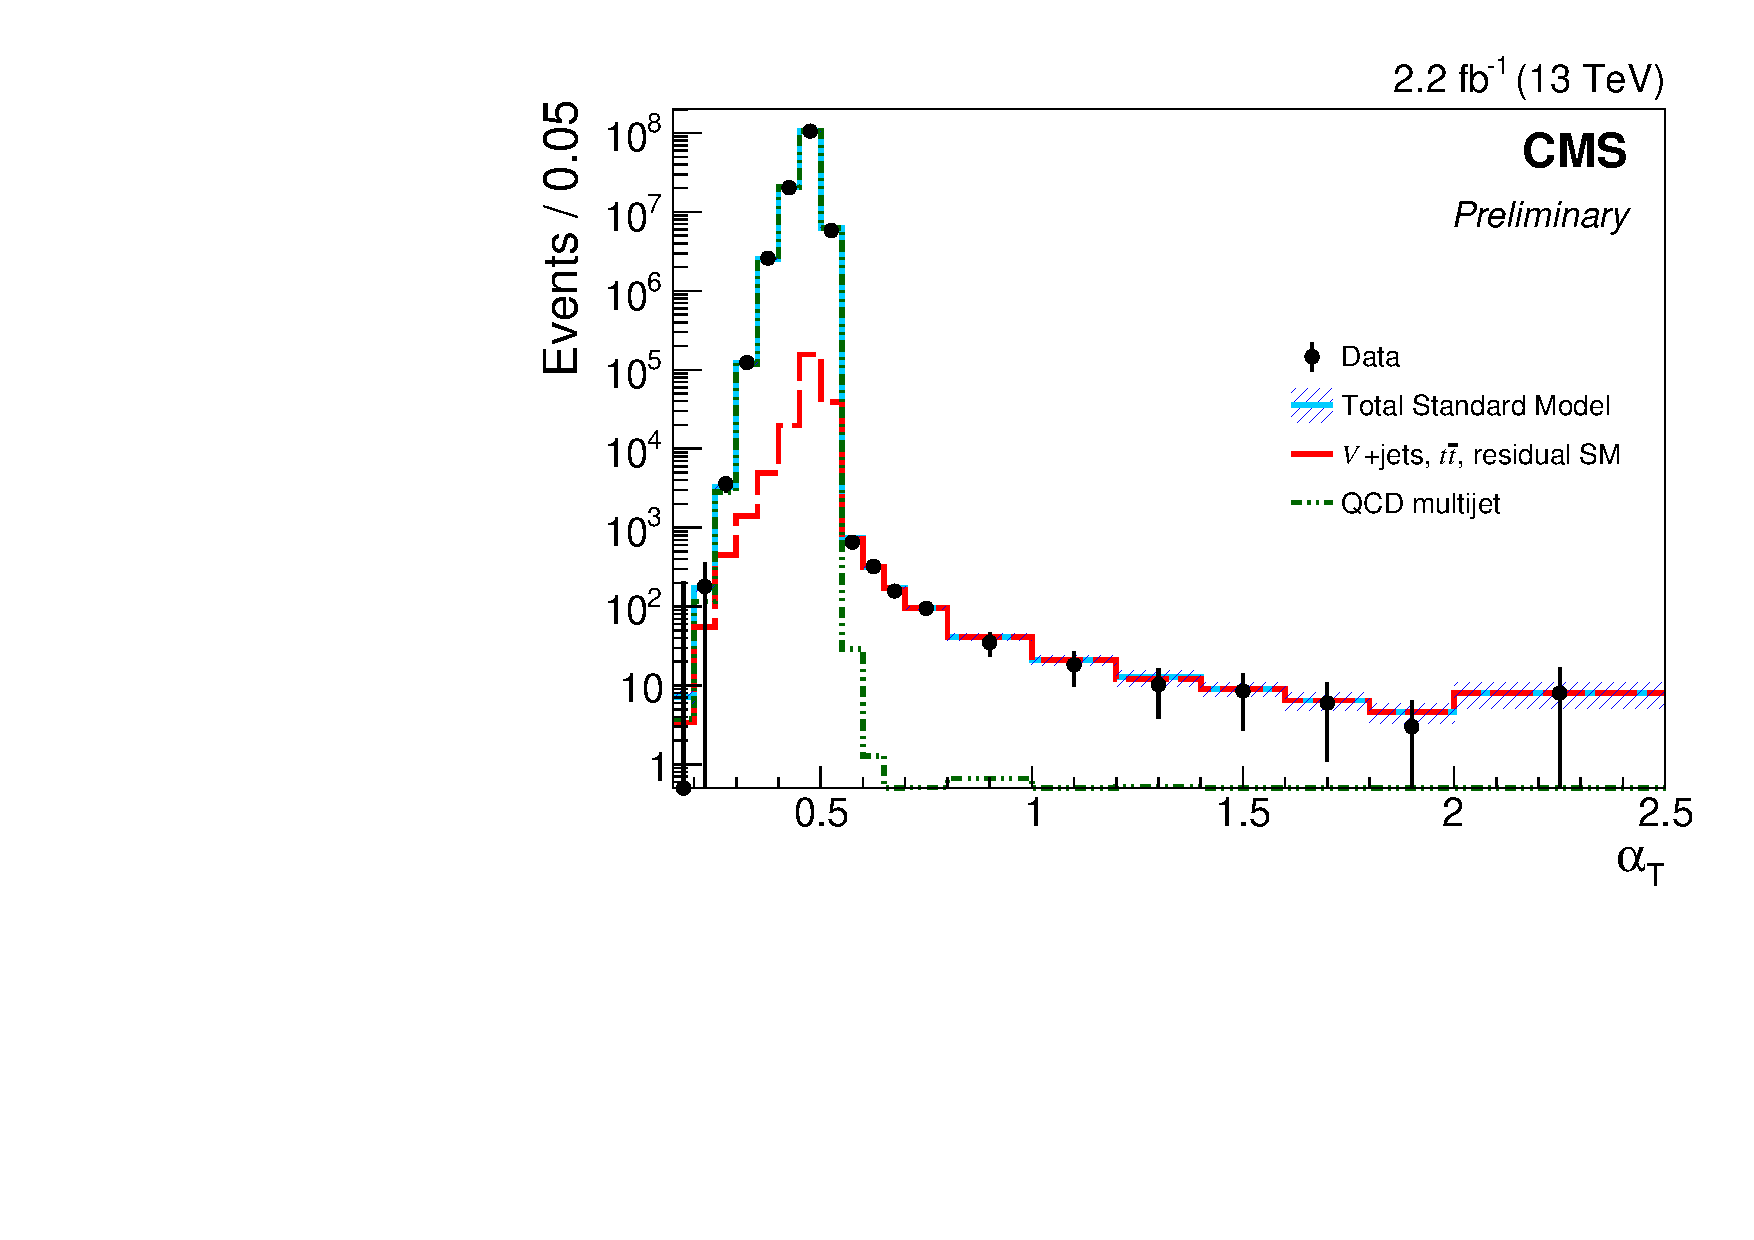
\includegraphics[width=0.5\textwidth]{figures/strategy/alphaT_v4.pdf}} ~~
        \caption{\alphat~variable for the 2015 $13$~TeV data set of $2.2$\ifb}
        \label{fig:strategy_alphaT}
    \end{center}
\end{figure}


Another dedicated variable used is 'biased $\Delta \Phi$' (\bdphi) which is the minimal opening angle between any jet and the \mht vector without considering the tagged jet. This variable is more robust against mis-measurements of the jets compared to the traditional $\temrm{min}\Delta \Phi$ variable and leads to shorter tails as shown in Fig.~\ref{fig:strategy_bdphi}.

 \begin{figure}
    \begin{center}
        \subfigure {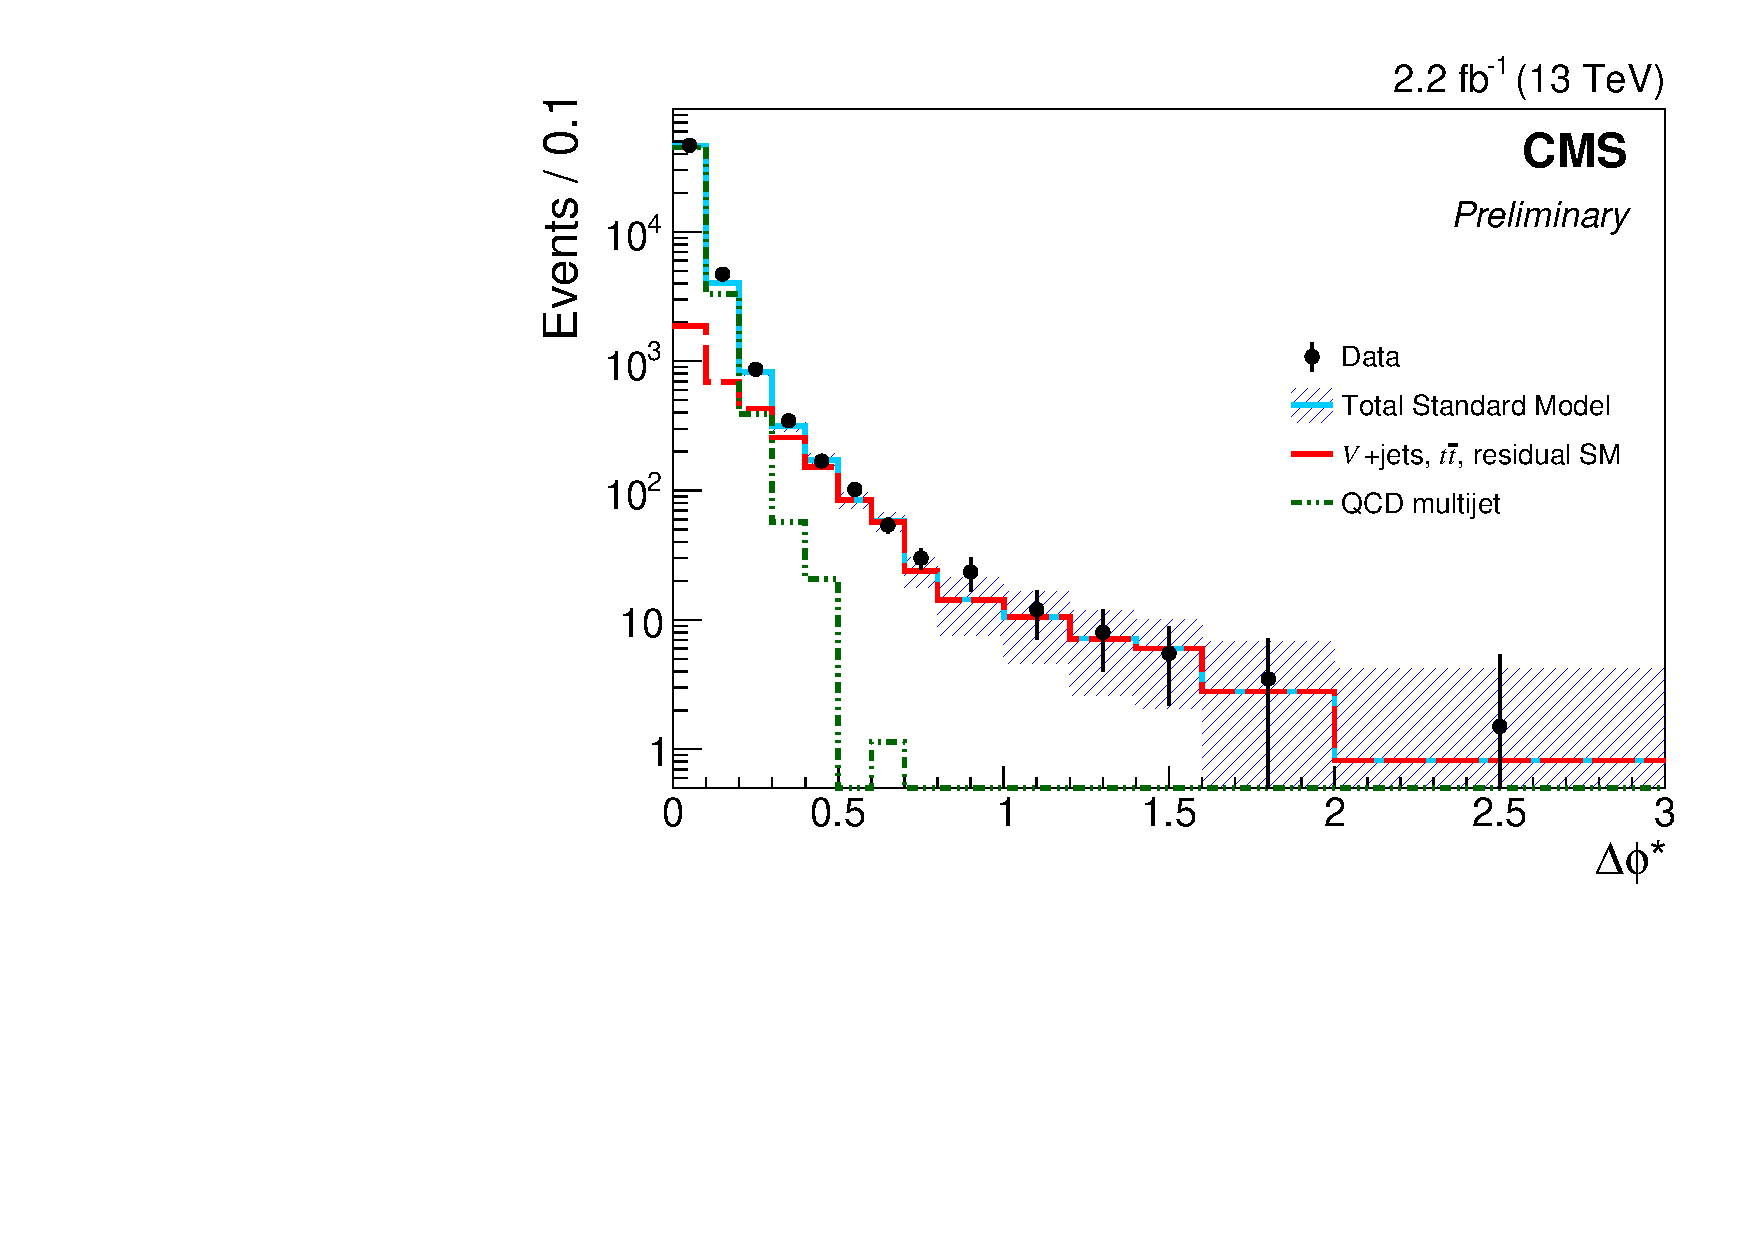
\includegraphics[width=0.5\textwidth]{figures/strategy/bDPhi_v4.pdf}}
        \caption{\bdphi~variable for the 2015 $13$~TeV data set of $2.2$\ifb}
        \label{fig:strategy_bdphi}
    \end{center}
\end{figure}


%%____________________________________________________________________________||
\section{Data sets}
\label{sec:datasets}

\subsection{Data}


In this note, we use 6.3~\ifb of proton-proton collision data at
$\sqrt{s} =$ 13~TeV collected in 2016. The JSON file listed in
Table~\ref{tab:cert_json} specifies the periods of the time in which
these certified data are collected. Table~\ref{tab:datasets_data} lists
the names of the data sets.

We perform a blind analysis; the data in the signal region was blinded
with the exception of 0.8~\ifb of the certified data specified by the
JSON file in Table~\ref{tab:cert_unblind_json}. Data in the control
regions is never blinded. These blinding policies are agree in the SUS
PAG.

During the review in the SUS PAG, it becomes clear that we understand
the data in the control regions and a small fraction of the unblinded
data in the signal region well enough to predict the backgrounds in
the signal region. As a result, no data in the signal region is
blinded in this version of the note.

\begin{table}[!h]
\topcaption{The JSON file that specifies the periods of the time in
which 6.3~\ifb of the certified data are collected} \footnotesize
%latex.default(d, title = NULL, booktabs = FALSE, width = 3, rowname = NULL,     helvetica = FALSE, caption.loc = "bottom", ...)%
\begin{center}
\begin{tabular}{c}
\hline\hline
\verb!Cert_271036-276811_13TeV_PromptReco_Collisions16_JSON.txt!\tabularnewline
\hline
\end{tabular}\end{center}
 \label{tab:cert_json}
\end{table}

\begin{table}[!h]
\topcaption{Data sets}
\footnotesize \begin{center}
\begin{tabular}{l}
\hline\hline
\multicolumn{1}{c}{Data set}\tabularnewline
\hline
\verb!/HTMHT/Run2016B-23Sep2016-v3/MINIAOD!\tabularnewline
\verb!/HTMHT/Run2016C-23Sep2016-v1/MINIAOD!\tabularnewline
\verb!/HTMHT/Run2016D-23Sep2016-v1/MINIAOD!\tabularnewline
\verb!/HTMHT/Run2016E-23Sep2016-v1/MINIAOD!\tabularnewline
\verb!/HTMHT/Run2016F-23Sep2016-v1/MINIAOD!\tabularnewline
\verb!/HTMHT/Run2016G-23Sep2016-v2/MINIAOD!\tabularnewline
\verb!/HTMHT/Run2016H-PromptReco-v2/MINIAOD!\tabularnewline
\verb!/HTMHT/Run2016H-PromptReco-v3/MINIAOD!\tabularnewline
\verb!/JetHT/Run2016B-23Sep2016-v2/MINIAOD!\tabularnewline
\verb!/JetHT/Run2016C-23Sep2016-v2/MINIAOD!\tabularnewline
\verb!/JetHT/Run2016D-23Sep2016-v2/MINIAOD!\tabularnewline
\verb!/JetHT/Run2016E-23Sep2016-v1/MINIAOD!\tabularnewline
\verb!/JetHT/Run2016F-23Sep2016-v1/MINIAOD!\tabularnewline
\verb!/JetHT/Run2016G-23Sep2016-v2/MINIAOD!\tabularnewline
\verb!/JetHT/Run2016H-PromptReco-v2/MINIAOD!\tabularnewline
\verb!/JetHT/Run2016H-PromptReco-v3/MINIAOD!\tabularnewline
\verb!/MET/Run2016B-23Sep2016-v3/MINIAOD!\tabularnewline
\verb!/MET/Run2016C-23Sep2016-v1/MINIAOD!\tabularnewline
\verb!/MET/Run2016D-23Sep2016-v1/MINIAOD!\tabularnewline
\verb!/MET/Run2016E-23Sep2016-v1/MINIAOD!\tabularnewline
\verb!/MET/Run2016F-23Sep2016-v1/MINIAOD!\tabularnewline
\verb!/MET/Run2016G-23Sep2016-v1/MINIAOD!\tabularnewline
\verb!/MET/Run2016H-PromptReco-v2/MINIAOD!\tabularnewline
\verb!/SingleMuon/Run2016B-23Sep2016-v3/MINIAOD!\tabularnewline
\verb!/SingleMuon/Run2016C-23Sep2016-v1/MINIAOD!\tabularnewline
\verb!/SingleMuon/Run2016D-23Sep2016-v1/MINIAOD!\tabularnewline
\verb!/SingleMuon/Run2016E-23Sep2016-v1/MINIAOD!\tabularnewline
\verb!/SingleMuon/Run2016F-23Sep2016-v1/MINIAOD!\tabularnewline
\verb!/SingleMuon/Run2016G-23Sep2016-v1/MINIAOD!\tabularnewline
\verb!/SingleMuon/Run2016H-PromptReco-v2/MINIAOD!\tabularnewline
\verb!/SingleMuon/Run2016H-PromptReco-v3/MINIAOD!\tabularnewline
\verb!/SinglePhoton/Run2016B-23Sep2016-v3/MINIAOD!\tabularnewline
\verb!/SinglePhoton/Run2016C-23Sep2016-v1/MINIAOD!\tabularnewline
\verb!/SinglePhoton/Run2016D-23Sep2016-v1/MINIAOD!\tabularnewline
\verb!/SinglePhoton/Run2016E-23Sep2016-v1/MINIAOD!\tabularnewline
\verb!/SinglePhoton/Run2016F-23Sep2016-v1/MINIAOD!\tabularnewline
\verb!/SinglePhoton/Run2016G-23Sep2016-v1/MINIAOD!\tabularnewline
\verb!/SinglePhoton/Run2016H-PromptReco-v2/MINIAOD!\tabularnewline
\verb!/SinglePhoton/Run2016H-PromptReco-v3/MINIAOD!\tabularnewline
\verb!/DoubleEG/Run2016B-23Sep2016-v3/MINIAOD!\tabularnewline
\verb!/DoubleEG/Run2016C-23Sep2016-v1/MINIAOD!\tabularnewline
\verb!/DoubleEG/Run2016D-23Sep2016-v1/MINIAOD!\tabularnewline
\verb!/DoubleEG/Run2016E-23Sep2016-v1/MINIAOD!\tabularnewline
\verb!/DoubleEG/Run2016F-23Sep2016-v1/MINIAOD!\tabularnewline
\verb!/DoubleEG/Run2016G-23Sep2016-v1/MINIAOD!\tabularnewline
\verb!/DoubleEG/Run2016H-PromptReco-v2/MINIAOD!\tabularnewline
\verb!/DoubleEG/Run2016H-PromptReco-v3/MINIAOD!\tabularnewline
\hline
\end{tabular}\end{center}

\label{tab:datasets_data}
\end{table}

\begin{table}[!h]
\topcaption{The JSON file specifying the 0.8~\ifb of the certified
data that we never blind} \footnotesize
%latex.default(d, title = NULL, booktabs = FALSE, width = 3, rowname = NULL,     helvetica = FALSE, caption.loc = "bottom", ...)%
\begin{center}
\begin{tabular}{c}
\hline\hline
 \verb!Cert_246908-257599_13TeV_PromptReco_Collisions15_25ns_JSON_v3.txt!\tabularnewline
\hline
\end{tabular}\end{center}

\label{tab:cert_unblind_json}
\end{table}

\subsection{Simulation}

Table~\ref{tab:datasets_bkg} lists the data sets of simulated events
of the standard model background processes used in this note. In these
data sets, in addition to the main interaction, each event contains on
average 20 minimum bias interactions which simulate multiple
interactions per bunch-crossing (in-time pileup). The expected
detector signal from previous or following bunch crossings
(out-of-time pileup) with 25ns bunch spacing is overlapped.

\begin{table}[!h]
 \centering
 \topcaption{Simulated background samples}
 \tiny
 \scalebox{.7}[1.0]{%latex.default(d, title = NULL, booktabs = FALSE, width = 3, rowname = NULL,     helvetica = FALSE, caption.loc = "bottom", ...)%
\begin{center}
\begin{tabular}{ll}
\hline\hline
\multicolumn{1}{c}{Data set}&\multicolumn{1}{c}{Cross section [pb]}\tabularnewline
\hline
\verb!/DYJetsToLL_M-10to50_TuneCUETP8M1_13TeV-amcatnloFXFX-pythia8/RunIISpring15DR74-Asympt25ns_MCRUN2_74_V9-v1/MINIAODSIM! &$1.861\times 10^{+04}$\tabularnewline
\verb!/DYJetsToLL_M-50_TuneCUETP8M1_13TeV-amcatnloFXFX-pythia8/RunIISpring15DR74-Asympt25ns_MCRUN2_74_V9-v3/MINIAODSIM! &$6.024\times 10^{+03}$\tabularnewline
\verb!/DYJetsToLL_M-50_HT-100to200_TuneCUETP8M1_13TeV-madgraphMLM-pythia8/RunIISpring15DR74-Asympt25ns_MCRUN2_74_V9-v2/MINIAODSIM! &$1.715\times 10^{+02}$\tabularnewline
\verb!/DYJetsToLL_M-50_HT-200to400_TuneCUETP8M1_13TeV-madgraphMLM-pythia8/RunIISpring15DR74-Asympt25ns_MCRUN2_74_V9-v2/MINIAODSIM! &$5.258\times 10^{+01}$\tabularnewline
\verb!/DYJetsToLL_M-50_HT-400to600_TuneCUETP8M1_13TeV-madgraphMLM-pythia8/RunIISpring15DR74-Asympt25ns_MCRUN2_74_V9-v2/MINIAODSIM! &$6.761\times 10^{+00}$\tabularnewline
\verb!/DYJetsToLL_M-50_HT-600toInf_TuneCUETP8M1_13TeV-madgraphMLM-pythia8/RunIISpring15DR74-Asympt25ns_MCRUN2_74_V9-v2/MINIAODSIM! &$2.718\times 10^{+00}$\tabularnewline
\verb!/GJets_HT-40To100_TuneCUETP8M1_13TeV-madgraphMLM-pythia8/RunIISpring15DR74-Asympt25ns_MCRUN2_74_V9-v2/MINIAODSIM! &$2.308\times 10^{+04}$\tabularnewline
\verb!/GJets_HT-100To200_TuneCUETP8M1_13TeV-madgraphMLM-pythia8/RunIISpring15DR74-Asympt25ns_MCRUN2_74_V9-v2/MINIAODSIM! &$9.110\times 10^{+03}$\tabularnewline
\verb!/GJets_HT-200To400_TuneCUETP8M1_13TeV-madgraphMLM-pythia8/RunIISpring15DR74-Asympt25ns_MCRUN2_74_V9-v2/MINIAODSIM! &$2.298\times 10^{+03}$\tabularnewline
\verb!/GJets_HT-400To600_TuneCUETP8M1_13TeV-madgraphMLM-pythia8/RunIISpring15DR74-Asympt25ns_MCRUN2_74_V9-v1/MINIAODSIM! &$2.730\times 10^{+02}$\tabularnewline
\verb!/GJets_HT-600ToInf_TuneCUETP8M1_13TeV-madgraphMLM-pythia8/RunIISpring15DR74-Asympt25ns_MCRUN2_74_V9-v1/MINIAODSIM! &$9.450\times 10^{+01}$\tabularnewline
\verb!/QCD_HT100to200_TuneCUETP8M1_13TeV-madgraphMLM-pythia8/RunIISpring15DR74-Asympt25ns_MCRUN2_74_V9-v2/MINIAODSIM! &$2.754\times 10^{+07}$\tabularnewline
\verb!/QCD_HT200to300_TuneCUETP8M1_13TeV-madgraphMLM-pythia8/RunIISpring15DR74-Asympt25ns_MCRUN2_74_V9-v2/MINIAODSIM! &$1.735\times 10^{+06}$\tabularnewline
\verb!/QCD_HT300to500_TuneCUETP8M1_13TeV-madgraphMLM-pythia8/RunIISpring15DR74-Asympt25ns_MCRUN2_74_V9-v2/MINIAODSIM! &$3.670\times 10^{+05}$\tabularnewline
\verb!/QCD_HT500to700_TuneCUETP8M1_13TeV-madgraphMLM-pythia8/RunIISpring15DR74-Asympt25ns_MCRUN2_74_V9-v1/MINIAODSIM! &$2.940\times 10^{+04}$\tabularnewline
\verb!/QCD_HT700to1000_TuneCUETP8M1_13TeV-madgraphMLM-pythia8/RunIISpring15DR74-Asympt25ns_MCRUN2_74_V9-v1/MINIAODSIM! &$6.524\times 10^{+03}$\tabularnewline
\verb!/QCD_HT1000to1500_TuneCUETP8M1_13TeV-madgraphMLM-pythia8/RunIISpring15DR74-Asympt25ns_MCRUN2_74_V9-v2/MINIAODSIM! &$1.064\times 10^{+03}$\tabularnewline
\verb!/QCD_HT1500to2000_TuneCUETP8M1_13TeV-madgraphMLM-pythia8/RunIISpring15DR74-Asympt25ns_MCRUN2_74_V9-v1/MINIAODSIM! &$1.215\times 10^{+02}$\tabularnewline
\verb!/QCD_HT2000toInf_TuneCUETP8M1_13TeV-madgraphMLM-pythia8/RunIISpring15DR74-Asympt25ns_MCRUN2_74_V9-v1/MINIAODSIM! &$2.542\times 10^{+01}$\tabularnewline
\verb!/QCD_Pt_80to120_TuneCUETP8M1_13TeV_pythia8/RunIISpring15DR74-Asympt25ns_MCRUN2_74_V9-v1/MINIAODSIM! &$2.763\times 10^{+06}$\tabularnewline
\verb!/QCD_Pt_120to170_TuneCUETP8M1_13TeV_pythia8/RunIISpring15DR74-Asympt25ns_MCRUN2_74_V9-v1/MINIAODSIM! &$4.711\times 10^{+05}$\tabularnewline
\verb!/QCD_Pt_170to300_TuneCUETP8M1_13TeV_pythia8/RunIISpring15DR74-Asympt25ns_MCRUN2_74_V9-v2/MINIAODSIM! &$1.173\times 10^{+05}$\tabularnewline
\verb!/QCD_Pt_300to470_TuneCUETP8M1_13TeV_pythia8/RunIISpring15DR74-Asympt25ns_MCRUN2_74_V9-v1/MINIAODSIM! &$7.823\times 10^{+03}$\tabularnewline
\verb!/QCD_Pt_470to600_TuneCUETP8M1_13TeV_pythia8/RunIISpring15DR74-Asympt25ns_MCRUN2_74_V9-v2/MINIAODSIM! &$6.482\times 10^{+02}$\tabularnewline
\verb!/QCD_Pt_600to800_TuneCUETP8M1_13TeV_pythia8/RunIISpring15DR74-Asympt25ns_MCRUN2_74_V9-v2/MINIAODSIM! &$1.869\times 10^{+02}$\tabularnewline
\verb!/QCD_Pt_800to1000_TuneCUETP8M1_13TeV_pythia8/RunIISpring15DR74-Asympt25ns_MCRUN2_74_V9-v2/MINIAODSIM! &$3.229\times 10^{+01}$\tabularnewline
\verb!/QCD_Pt_1000to1400_TuneCUETP8M1_13TeV_pythia8/RunIISpring15DR74-Asympt25ns_MCRUN2_74_V9-v1/MINIAODSIM! &$9.418\times 10^{+00}$\tabularnewline
\verb!/QCD_Pt_1400to1800_TuneCUETP8M1_13TeV_pythia8/RunIISpring15DR74-Asympt25ns_MCRUN2_74_V9-v1/MINIAODSIM! &$8.427\times 10^{-01}$\tabularnewline
\verb!/QCD_Pt_1800to2400_TuneCUETP8M1_13TeV_pythia8/RunIISpring15DR74-Asympt25ns_MCRUN2_74_V9-v1/MINIAODSIM! &$1.149\times 10^{-01}$\tabularnewline
\verb!/QCD_Pt_2400to3200_TuneCUETP8M1_13TeV_pythia8/RunIISpring15DR74-Asympt25ns_MCRUN2_74_V9-v1/MINIAODSIM! &$6.830\times 10^{-03}$\tabularnewline
\verb!/QCD_Pt_3200toInf_TuneCUETP8M1_13TeV_pythia8/RunIISpring15DR74-Asympt25ns_MCRUN2_74_V9-v1/MINIAODSIM! &$1.654\times 10^{-04}$\tabularnewline
\verb!/ST_tW_antitop_5f_inclusiveDecays_13TeV-powheg-pythia8_TuneCUETP8M1/RunIISpring15DR74-Asympt25ns_MCRUN2_74_V9-v1/MINIAODSIM! &$3.560\times 10^{+01}$\tabularnewline
\verb!/TTJets_TuneCUETP8M1_13TeV-amcatnloFXFX-pythia8/RunIISpring15DR74-Asympt25ns_MCRUN2_74_V9-v1/MINIAODSIM! &$8.318\times 10^{+02}$\tabularnewline
\verb!/TTJets_TuneCUETP8M1_13TeV-madgraphMLM-pythia8/RunIISpring15DR74-Asympt25ns_MCRUN2_74_V9-v2/MINIAODSIM! &$8.318\times 10^{+02}$\tabularnewline
\verb!/ST_s-channel_4f_leptonDecays_13TeV-amcatnlo-pythia8_TuneCUETP8M1/RunIISpring15DR74-Asympt25ns_MCRUN2_74_V9-v1/MINIAODSIM! &$3.681\times 10^{+00}$\tabularnewline
\verb!/ST_t-channel_4f_leptonDecays_13TeV-amcatnlo-pythia8_TuneCUETP8M1/RunIISpring15DR74-Asympt25ns_MCRUN2_74_V9-v1/MINIAODSIM! &$7.031\times 10^{+01}$\tabularnewline
\verb!/ST_tW_top_5f_inclusiveDecays_13TeV-powheg-pythia8_TuneCUETP8M1/RunIISpring15DR74-Asympt25ns_MCRUN2_74_V9-v1/MINIAODSIM! &$3.560\times 10^{+01}$\tabularnewline
\verb!/WJetsToLNu_TuneCUETP8M1_13TeV-amcatnloFXFX-pythia8/RunIISpring15DR74-Asympt25ns_MCRUN2_74_V9-v1/MINIAODSIM! &$6.153\times 10^{+04}$\tabularnewline
\verb!/WJetsToLNu_HT-100To200_TuneCUETP8M1_13TeV-madgraphMLM-pythia8/RunIISpring15DR74-Asympt25ns_MCRUN2_74_V9-v1/MINIAODSIM! &$1.630\times 10^{+03}$\tabularnewline
\verb!/WJetsToLNu_HT-200To400_TuneCUETP8M1_13TeV-madgraphMLM-pythia8/RunIISpring15DR74-Asympt25ns_MCRUN2_74_V9-v1/MINIAODSIM! &$4.356\times 10^{+02}$\tabularnewline
\verb!/WJetsToLNu_HT-400To600_TuneCUETP8M1_13TeV-madgraphMLM-pythia8/RunIISpring15DR74-Asympt25ns_MCRUN2_74_V9-v3/MINIAODSIM! &$5.917\times 10^{+01}$\tabularnewline
\verb!/WJetsToLNu_HT-600To800_TuneCUETP8M1_13TeV-madgraphMLM-pythia8/RunIISpring15DR74-Asympt25ns_MCRUN2_74_V9-v2/MINIAODSIM! &$1.549\times 10^{+01}$\tabularnewline
\verb!/WJetsToLNu_HT-800To1200_TuneCUETP8M1_13TeV-madgraphMLM-pythia8/RunIISpring15DR74-Asympt25ns_MCRUN2_74_V9-v1/MINIAODSIM! &$6.365\times 10^{+00}$\tabularnewline
\verb!/WJetsToLNu_HT-1200To2500_TuneCUETP8M1_13TeV-madgraphMLM-pythia8/RunIISpring15DR74-Asympt25ns_MCRUN2_74_V9-v1/MINIAODSIM! &$1.609\times 10^{+00}$\tabularnewline
\verb!/WJetsToLNu_HT-2500ToInf_TuneCUETP8M1_13TeV-madgraphMLM-pythia8/RunIISpring15DR74-Asympt25ns_MCRUN2_74_V9-v2/MINIAODSIM! &$3.738\times 10^{-02}$\tabularnewline
\verb!/WWTo2L2Nu_13TeV-powheg/RunIISpring15DR74-Asympt25ns_MCRUN2_74_V9-v1/MINIAODSIM! &$1.246\times 10^{+01}$\tabularnewline
\verb!/WZ_TuneCUETP8M1_13TeV-pythia8/RunIISpring15DR74-Asympt25ns_MCRUN2_74_V9-v1/MINIAODSIM! &$6.610\times 10^{+01}$\tabularnewline
\verb!/ZJetsToNuNu_HT-100To200_13TeV-madgraph/RunIISpring15DR74-Asympt25ns_MCRUN2_74_V9-v1/MINIAODSIM! &$3.450\times 10^{+02}$\tabularnewline
\verb!/ZJetsToNuNu_HT-200To400_13TeV-madgraph/RunIISpring15DR74-Asympt25ns_MCRUN2_74_V9-v1/MINIAODSIM! &$9.638\times 10^{+01}$\tabularnewline
\verb!/ZJetsToNuNu_HT-400To600_13TeV-madgraph/RunIISpring15DR74-Asympt25ns_MCRUN2_74_V9-v1/MINIAODSIM! &$1.346\times 10^{+01}$\tabularnewline
\verb!/ZJetsToNuNu_HT-600ToInf_13TeV-madgraph/RunIISpring15DR74-Asympt25ns_MCRUN2_74_V9-v1/MINIAODSIM! &$5.170\times 10^{+00}$\tabularnewline
\verb!/ZZ_TuneCUETP8M1_13TeV-pythia8/RunIISpring15DR74-Asympt25ns_MCRUN2_74_V9-v3/MINIAODSIM! &$3.180\times 10^{+01}$\tabularnewline
\hline
\end{tabular}\end{center}
}
 \label{tab:datasets_bkg}
\end{table}


\clearpage

\subsection{Pileup reweighting}
\label{sec:pileup-reweighting}

The distribution of the numbers of the pileup interactions in the
simulated events is different from that in the data; the simulated
events contain, on average, a larger number of pileup interactions than
the data. We reweight simulated events to correct for this difference.
This procedure is called \textit{pileup reweighting}.

In deriving the pileup reweighting factors, we follow the
recommendation by the physics validation group
\cite{twiki-PdmVPileUpDescription, twiki-PileupJSONFileforData}. In
the recommendation, the reweighting factors are a function of the
variable called \verb!nTrueInt!.

This variable \verb!nTrueInt! is the parameter of the Poisson
distribution from which the numbers of pileup interactions are drown
as random numbers. In each simulated event, the number of the in-time
pileup interactions and the number of the interactions in each
neighbouring bunch crossing to simulate the out-of-time pileup are
random numbers from the Poisson distribution with the same parameter,
\verb!nTrueInt!. The value of \verb!nTrueInt! is not a constant of the
data set. It is a random number from the distribution specified in
Ref. \cite{github-mix_2016_25ns_SpringMC_PUScenarioV1_PoissonOOTPU_cfi}.

The \verb!nTrueInt! in the data is the average pileup interactions for
a colliding bunch pair in a lumi section. The distribution of
\verb!nTrueInt! in the data is derived from the measured instantaneous
luminosity for each colliding bunch pair in each lumi section and the
cross section of the total inelastic pp interaction. We use the method
in Ref. \cite{twiki-PileupJSONFileforData} in deriving the
distribution with the recommended value of 71.3~mb as the minimum bias
cross section \cite{CMS-FSQ-15-005}.

The pileup reweighting factors are the ratios of the distributions of
\verb!nTrueInt! in the data and in the simulated events and are
normalised so as to preserve the number of the simulated events.

Figure~\ref{f044_corr_nTrueInt_data_mc_norm} shows the distributions
of \verb!nTrueInt! in the data, simulated events and reweighted
simulated events. The figure demonstrates that the reweighted
simulated events have the distribution of \verb!nTrueInt! nearly
identical to that in the data.

\begin{figure}[!b]
\centering
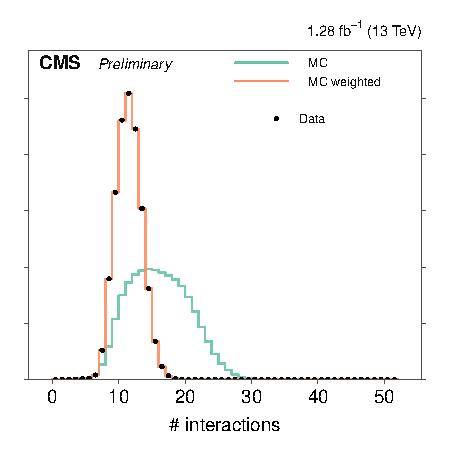
\includegraphics[scale=1.00]{figures/pileup_reweighting/f044_corr_nTrueInt_data_mc_norm}
\caption{The distribution of the average numbers of the inelastic
interactions per colliding bunch pair per lumi section in the data,
corresponding distribution in the simulated events, and that of the
reweighted simulated events.} \label{f044_corr_nTrueInt_data_mc_norm}
\end{figure}


\subsection{Cross sections for SM samples}
\label{sec:SMxs}
Several MC samples of individual SM processes are binned according to a generator level quantity, 
such as the partonic \HT or bosonic \PT.
This analysis chooses to use samples binned in partonic \HT 
for the set of MC samples (W+jets, DY+jets, QCD, $\gamma$+jets, $Z\rightarrow \nu\nu$+jets).
These binned samples are provided with LO cross sections. 
The \kfactors required to go from LO to NNLO cross section are typically determined using corresponding
inclusive samples applied to each \HT binned sample.
Further studies can provide additional corrections to the cross sections, 
which can prove important to the closure test procedures described in
Section \ref{sec:closure-tests}. As can be seen in Section~\ref{sec:sideband_corrections}, residual cross section
corrections are measured using data in sidebands designed to enrich specific processes.

In the $8\tev$ LHC results the shape of the top quark $p_{T}$ spectrum
was found to differ between simulation and data. A reweighting is
therefore applied to MC events that contain a generated top. The value of
this correction is provided from the $8\tev$ results, as described in
\cite{twiki-TopPtReweighting}.

The inclusive distributions of the MC samples
with respect to the binning variable
$H_{T}^{parton}$ are shown in Fig.~\ref{fig:Lhe_Ht}, with
the bin by bin derivative drawn below.

As can be seen in the distributions, the stitched samples
exhibit a good level of smoothness,
further demonstrated by the derivative which shows a flat trend for each 
cross section.

A more in depth and data-driven investigation of the cross sections is shown in Sec.~\ref{sec:sideband_corrections}. 
Of which, an important point to note is that the corrections to the cross sections, 
derived with the data sidebands are only relevant for Data/MC comparison plots and the suite of closure tests defined in Section \ref{sec:closure-tests}.

\begin{figure}[!h]
  \begin{center}
    \subfigure[$Z\rightarrow \nu\nu$ +jets] {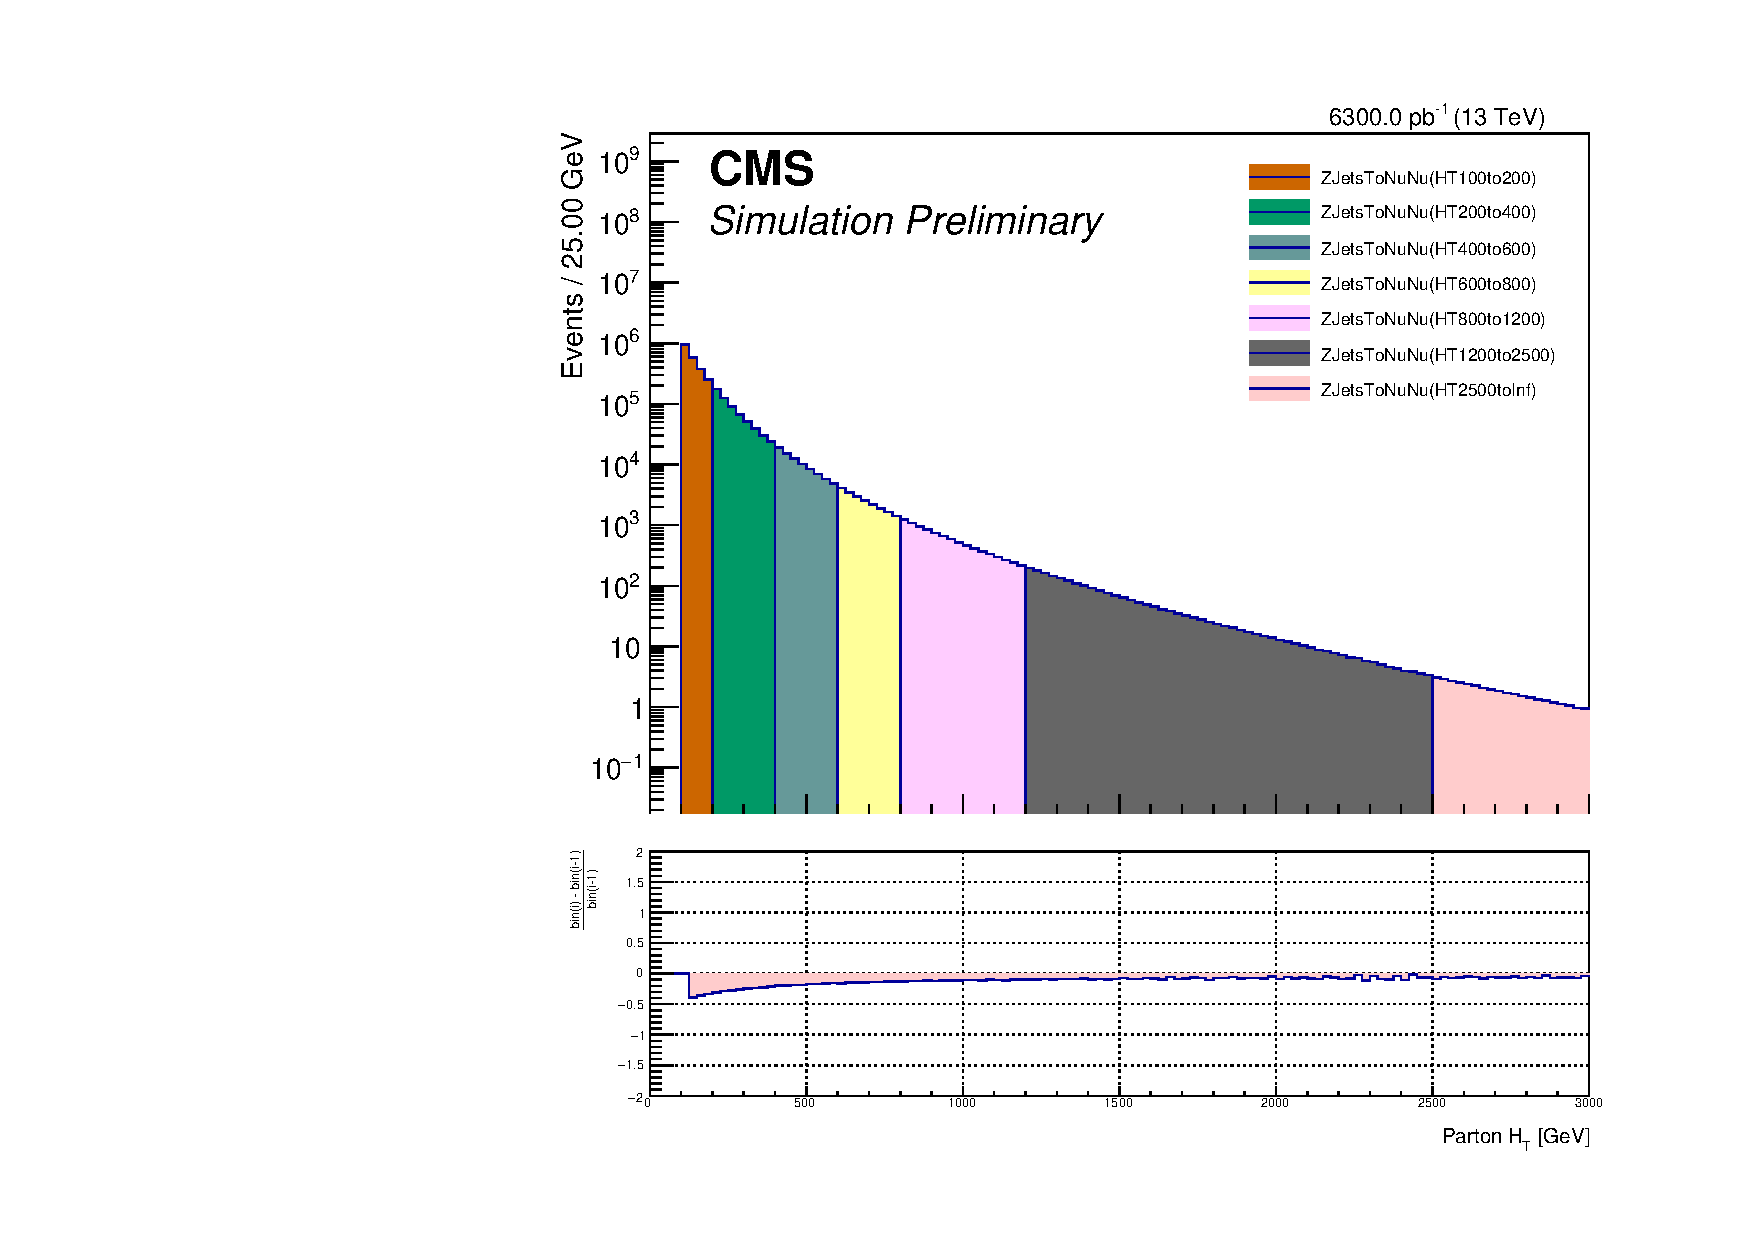
\includegraphics[width=0.40\textwidth]{figures/binnedMCsamples/2016/6p3/Zinv.pdf}} ~~
    \subfigure[$W\rightarrow l \nu$ + jets]{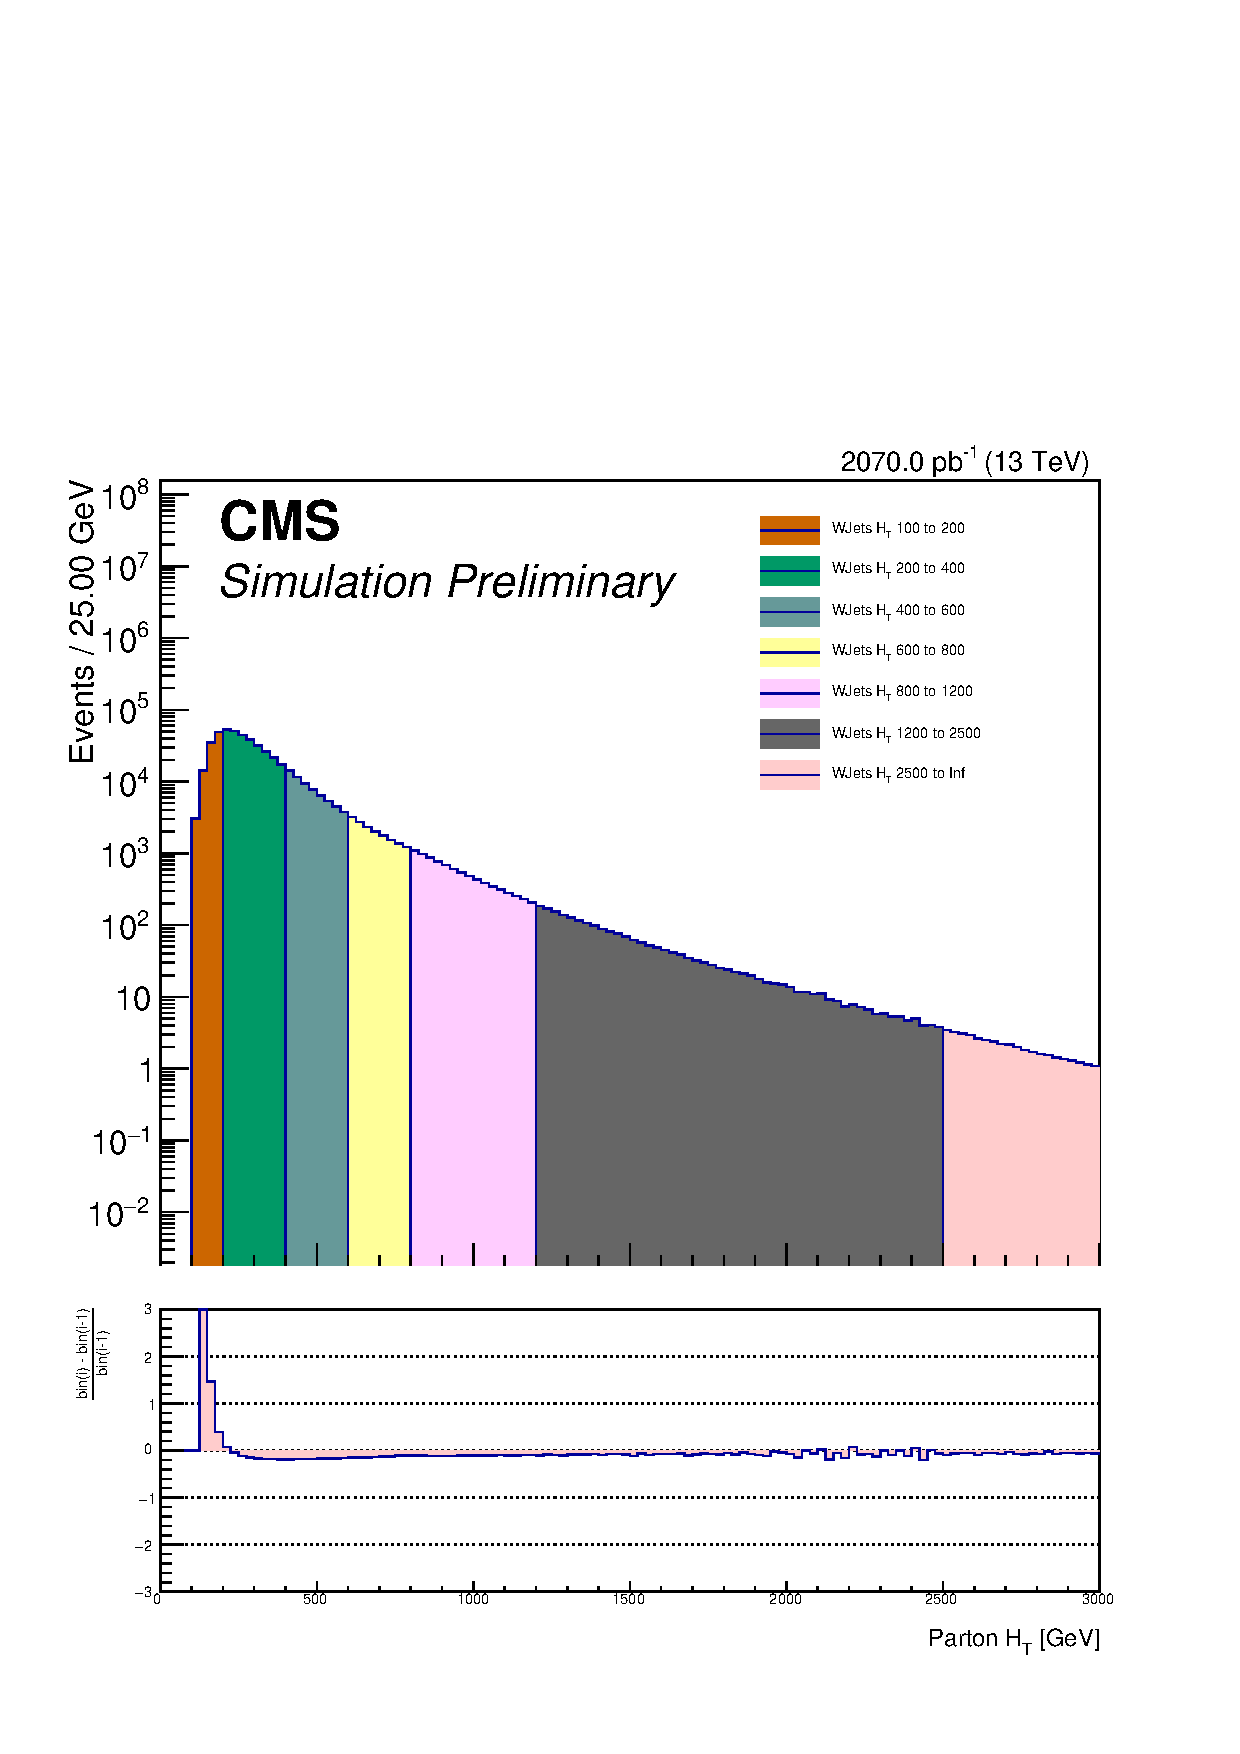
\includegraphics[width=0.40\textwidth]{figures/binnedMCsamples/2016/6p3/WJetsToLNu_HT.pdf}} \\
    \subfigure[$DY\rightarrow ll$ + jets]{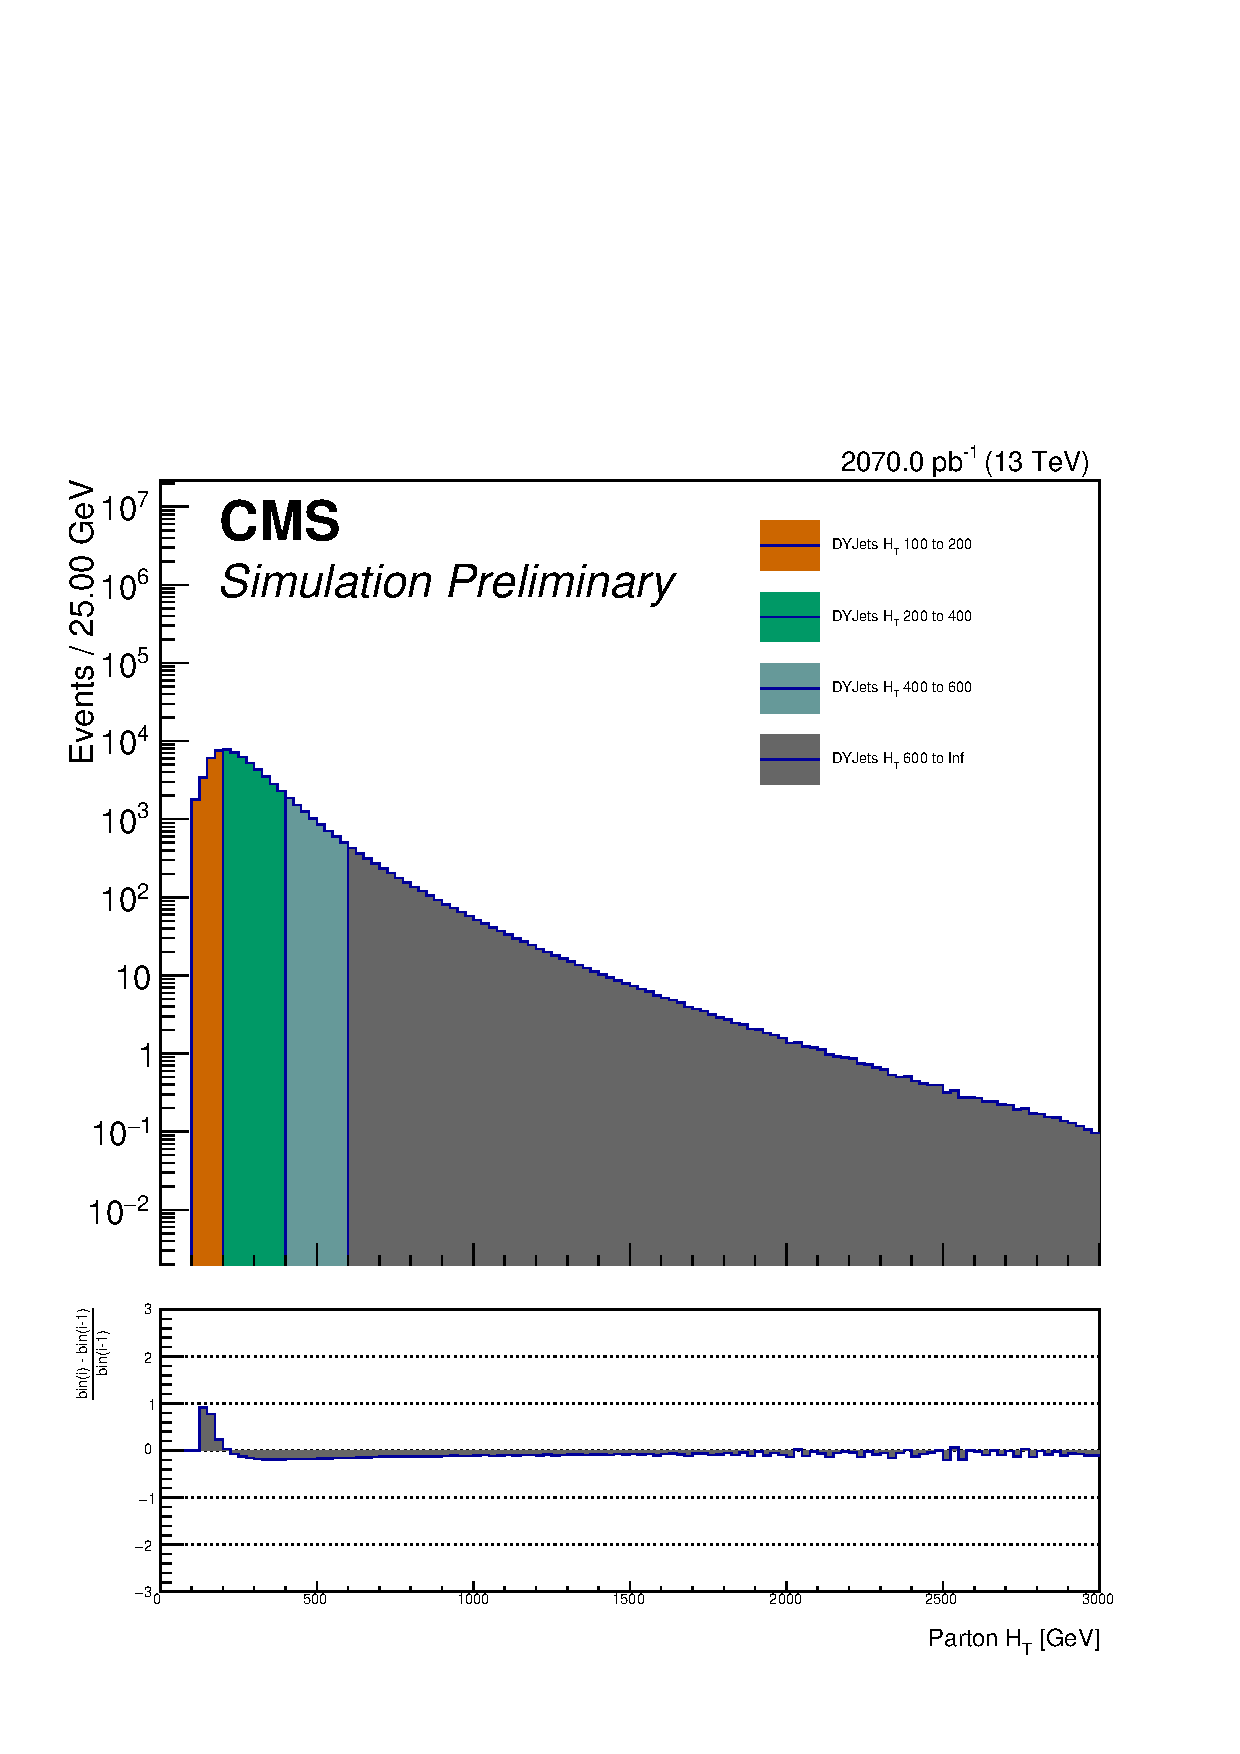
\includegraphics[width=0.40\textwidth]{figures/binnedMCsamples/2016/6p3/DYJetsToLL_M50_HT.pdf}} ~~
    \subfigure[QCD]{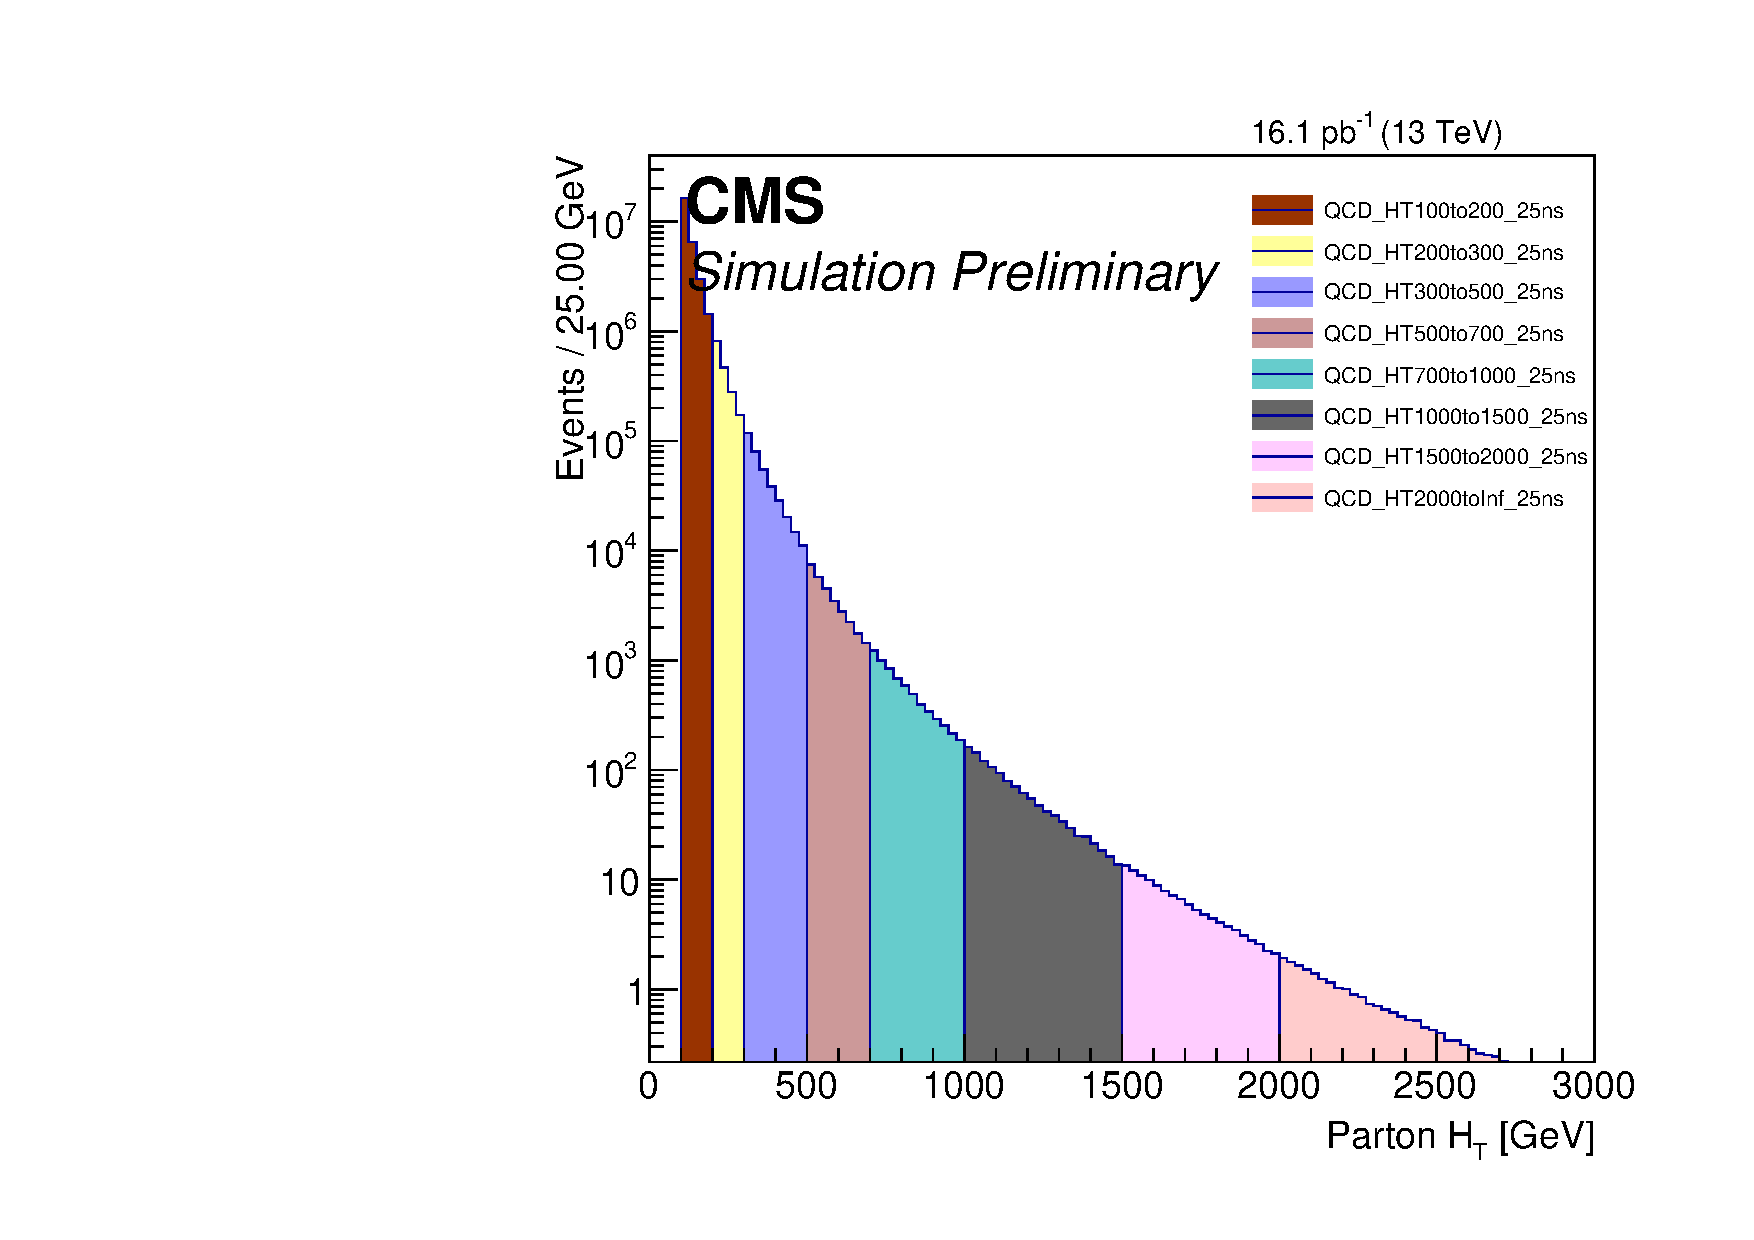
\includegraphics[width=0.40\textwidth]{figures/binnedMCsamples/2016/6p3/QCD_HT.pdf}} \\
    \subfigure[$\gamma$+jets]{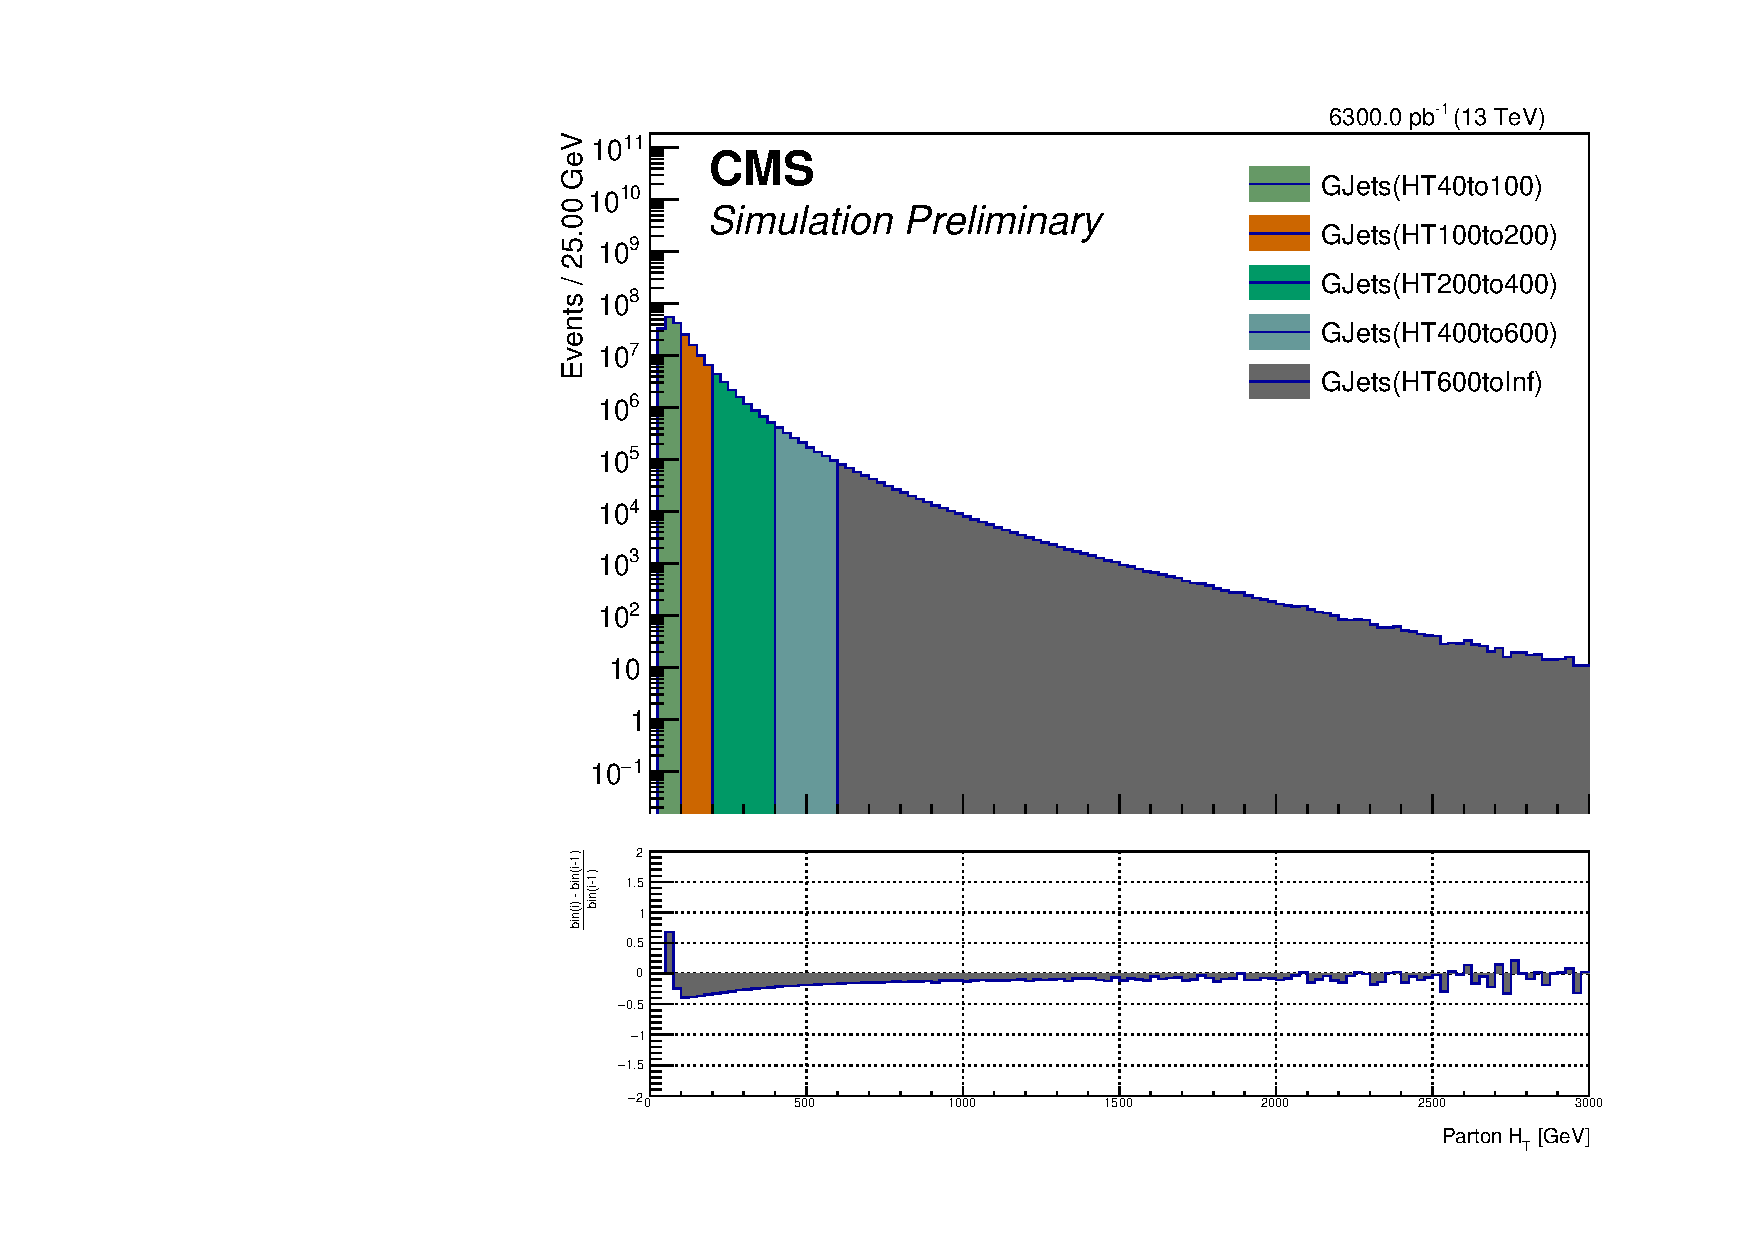
\includegraphics[width=0.40\textwidth]{figures/binnedMCsamples/2016/6p3/GJets_HT.pdf}} ~~
    \caption{Generator-level $H_{T}^{parton}$ distributions for SM process, $Z\rightarrow \nu\nu$ + jets, W+jets, DY+jets, QCD and $\gamma$+jets}
    \label{fig:Lhe_Ht}
  \end{center}
\end{figure}

%%____________________________________________________________________________||

%____________________________________________________________________________||
\section{Event selection for signal and control regions}
\label{sec:selection}

This section first outlines the set of ``pre-selection'' requirements
that are common to all signal and control regions, before defining the
selection criteria that are specific to each region.

%%____________________________________________________________________________||
\subsection{Pre-selection}
\label{sec:preSelection}

{\bf Removing instrumental sources of ``fake'' \met.} 

A number of beam- and detector-related effects can induce significant
\met. Examples include beam halo, reconstruction failures, spurious
detector noise, or event misreconstruction due to detector
inefficiencies. These events, with large, non-physical values of \met,
are rejected with high efficiency by applying a range of dedicated
vetoes. All ``MET filters'' recommended by the JetMET POG and SUSY PAG
are applied by default in this analysis and listed in Table~\ref{tab:pre-selections}.

{\bf Jet requirements.} 

Jets considered in the analysis are required to satisfy $\PT>40\gev$
and $|\eta|<3.0$. Events containing jets in the forward region that
satisfy the requirements $\PT>40\gev$ and $|\eta|>3.0$ are rejected in
order to control background contributions from SM processes, without
introducing a significant reduction in signal acceptance. The jets
that are selected are used in the calculation of all jet-based
event-level variables, such as \HT, \mht, and \alphat.

Raised $\PT$ thresholds and tighter $\eta$ requirements on the lead jets 
are also required. The lead jet is required to satisfy $\PT > 100\gev$
and $|\eta|<2.5$. This helps to ensure high trigger efficiencies,
but also helps to improve the S/B for a wide
range of models with respect to SM processes, such as V + jets
production. Events are then classified based on the
second leading jet. In the case that a second leading jet satisfies $\PT > 100\gev$ 
events are assigned to a ``symmetric'' \njet category. If the second
jet satisfies $40 < \PT < 100\gev$ events are assigned to an
``asymmetric'' \njet category. Finally, if there is no second leading
jet with $\PT>40\gev$, events are assigned to the ``mono-jet''
category. This categorisation is heavily utilised throughout all the document. \\
The asymmetric and mono-jet categories have been added to
the analysis to help improve acceptance to a range of DM models and compressed
SUSY.

{\bf Event categorisation according to \njet and \nb.} 

Events in the hadronic signal and all control regions (described
below) are categorised identically and according to the number of jets
(\njet) reconstructed in each event and the number of jets identified
as originating from bottom quarks (\nb) in each event. As a baseline,
the resulting sub-samples comprise events containing exactly one, two,
three, four, or at least five jets. These are further split into
``monojet'' (only in the $\njet=1$ case),
``symmetric'' or ``asymmetric'' \njet categories according to the
second leading jet \Pt, as defined above.

Events are also categorised according to the the number of b-tagged
jets (``b-jets''). As a baseline, the sub-samples are defined by
requiring exactly zero, one, two, or at least three b-tagged jets. By
construction, $\nb \leq \njet$. Standard Model background events containing three or more b-tags
typically arise from an additional source of b-jets like 
``gluon splitting'' or from 
mistag of a jet from a light-flavoured parton. 


{\bf \HT,\mht requirements and binning.} 

Events are required to have significant hadronic activity by requiring
$\scalht > 200\GeV$. Despite an increase in both multijet production
cross sections and pileup in Run~2, the lowest \HT threshold is
kept at the same value of the Run~1 analysis~\cite{Chatrchyan:2013lya}
in order to maintain acceptance to DM models or compressed
SUSY. Events in all samples are binned identically, according to the
\HT variable. The choice of binning in \HT is driven primarily by the
trigger strategy employed by the analysis, as described in
Section~\ref{sec:triggers}, and can be summarised as follows: 50\gev
bins in the range $200 < \HT < 400\gev$, 100\gev bins in the range
$400 < \HT < 600\gev$, a 200\gev bin $600<\HT<800\gev$ and a final 
inclusive bin $\HT > 800\gev$.

Events are also required to have appreciable missing hadronic energy
by requiring $\mht>130\gev$. This ensures that all events used within
the analysis have a degree of missing energy similar to that required
in the signal region via an \alphat cut. This is outlined in
Sec.~\ref{sec:had-signal}. 

The lower threshold of the last (inclusive) \HT bin is not forced to
$800\gev$, it is instead determined
independently for each (\njet,\nb) event category and is chosen to
always align with one of the ``default'' boundaries defined above. The
metric for choosing the final bin threshold is based on the number of
events in the corresponding event category and \HT bin of the data
control samples. This ensures that all bins in the data control
samples are sufficiently populated to ensure a statistically
significant prediction in each of the corresponding signal region
bins. Currently, this is achieved by requiring at least $10$ predicted
events in each \HT and \njet category of the control regions
along with the requirement that there is at least one observed
event per \nb category. If this is not the case, events from high \HT bins are combined
into a single inclusive bin that satisfies this metric. This metric
ensures that there are sufficient events in the control samples
to probe for potential systematic effects with closure tests between
simulation and data, as described in Sec.~\ref{sec:systematics}.

\begin{table}[h!]
  \topcaption{Summary of the pre-selection criteria.}
  \label{tab:pre-selections}
  \centering
  \footnotesize
  \begin{tabular}{ ll }
    \hline
    \hline
    Selection                     & Requirement                                                                          \\
    \hline
    ``MET filters''               & Primary Vertex, CSC Beam Halo, HBHE Noise and Isolation, ECAL Endcap SC Noise        \\
    Jet acceptance                & $\PT > 40\gev$, $|\eta| < 3$                                                         \\
%    \njet                         & $\geq2$                                                                \\
    Lead jet acceptance           & $\PT > 100\gev$, $|\eta| <    2.5$                                     \\
    Second jet acceptance         & $\PT > 100\gev$ \texttt{OR} $40 < \PT < 100\gev$                       \\
    Loosest \HT requirement       & $\HT > 200\gev$                                                        \\
    Loosest \mht requirement      & $>130\gev$                                                     \\  
    Baseline \HT binning          & 200--250, 250--300, 300--350, 350--400, 400--500, 500--600, 600--800, $>$800\gev \\
    Baseline \njet multiplicities & 1 (mono-jet), 2, 3, 4, $\geq$5 (both symmetric and asymmetric)                       \\
    Baseline \nb multiplicities   & 0, 1, 2, $\geq3$ ($\nb \leq \njet$)                                    \\
    \hline
    \hline
  \end{tabular}
\end{table}

{\bf Summary of pre-selection requirements.} 

Table~\ref{tab:pre-selections} summarises the pre-selection
requirements and default categorisation and binning scheme. The
threshold of the final \HT bin per (\njet,\nb) category is summarised
in Table~\ref{tab:binning-3fb}. An identical scheme is used for the
signal region and all control regions. No extrapolation is performed
in the variables \njet, \nb, and \HT in this analysis. For each of the
signal and control regions, thirty event categories are considered,
each with up to seven bins in \HT, assuming an integrated luminosity
of 2.1\ifb. 

\begin{table}[h!]
  \caption{Threshold (GeV) of the final \HT bin as a function of event
    category (\njet,\nb), which is always aligned with respect
    to one of the baseline boundaries (motivated primarily by the trigger) of
    200, 250, 300, 350, 400, 600, 800\gev. 
    %This is the projected choice for 3\fbinv.
    }
  \label{tab:binning-3fb}
  \centering
  \footnotesize
  \hspace*{-1cm}\begin{tabular}{ l|cc|ccc|cccc|cccc|cccc }
    \hline
    \hline
    \njet      & \multicolumn{2}{c|}{1} & \multicolumn{3}{c|}{2} & \multicolumn{4}{c|}{3} & \multicolumn{4}{c|}{4} & \multicolumn{4}{c}{$\geq5$} \\ 
    \nb        & 0   & 1   & 0   & 1   & 2   & 0   & 1   & 2   & 3   & 0   & 1   & 2   & $\geq3$ & 0   & 1   & 2   & $\geq3$ \\
    \hline
    Symmetric  & 600 & 500 & 800 & 800 & 600 & 800 & 800 & 800 & 400 & 800 & 800 & 800 & 800     & 800 & 800 & 800 & 800     \\
    Asymmetric & -   & -   & 600 & 500 & 400 & 600 & 600 & 500 & 300 & 600 & 600 & 600 & 400     & 600 & 600 & 600 & 500     \\
    \hline
    \hline
  \end{tabular}
\end{table}


\subsection{Lepton and photon vetoes \label{sec:vetoes}}

To select a sample of events in the hadronic final state and to
suppress SM processes with genuine \met from neutrinos, events
containing an isolated electron with $\pt > 10\GeV$ and $|\eta| < 2.5$
or an isolated muon with $\pt > 10\GeV$ and $|\eta| < 2.5$ are
vetoed. Further, to reduce the ``lost leptons'' backgrounds from \wj
and \ttbar, events containing single isolated tracks with $\pt >
10\GeV$ and $|\eta| < 2.5$, as defined in Sec.~\ref{sec:objects},
are vetoed as part of the signal region selection criteria. In the
case of the single and di-lepton control samples, a further
requirement is made such that events are not vetoed due to the
presence of a track from the well identified leptons, by requiring
$\Delta R(\textrm{track},\textrm{lepton}) > 0.02$.

Finally, to select a purely hadronic topology and to allow for a
orthogonal control region, events are vetoed in which an isolated photon
with $\pt > 25\GeV$ and $|\eta| < 2.5$ is identified.

\subsection{The hadronic signal region}
\label{sec:had-signal}

The lepton and photon vetoes are applied to select hadronic final
states. All pre-selection criteria are also applied. Following these
selections, the multijet background from QCD is still several orders
of magnitude larger than the typical signal expected from SUSY.

{\bf \HT-dependent \alphat requirements.}

Background events from multijet production populate the region
$\alphat \lesssim 0.5$ and therefore can be rejected with very high
efficiency by requiring an appropriate cut on \alphat. 

A useful approximate conversion between \alphat and \mht can be
obtained by calculating \alphat, as described by Eq.~\ref{eq:alphat3}, 
while forcing $\dht = 0\gev$,. Hence, using this metric, the
dependence of the \alphat requirement as a function of the \HT bin can
be determined such that the effective requirement on \mht is
comparable, \ie roughly constant, across all \HT bins. The values
typically fall in the range $\sim110 < \mht < \sim160\gev$. This
approximate levelling of the ``effective'' \mht threshold implies
increasingly tighter requirements against instrumental effects versus
\HT, while maximising signal
acceptance. Table~\ref{tab:alphat-thresholds} summarises the 
\alphat thresholds and corresponding ``effective'' \mht thresholds for
each \HT bin. The \alphat threshold is dependent only on \HT and not
on \njet nor \nb that are used to define the event categories.

\begin{table}[h!]
  \caption{\alphat and corresponding ``effective'' \mht (GeV) thresholds versus
    lower bound of \scalht bin. For all \HT bins satisfying $\HT > 800
    \gev$, the direct requirement of $\mht > 130\gev$ is imposed rather
    than a requirement on \alphat. No \alphat requirement is imposed in the
    monojet bins.}
  \label{tab:alphat-thresholds}
  \centering
  \footnotesize
  \begin{tabular}{ lcccccccc }
    \hline
    \hline
    \scalht            & 200       & 250       & 300       & 350       & 400       & 500       & 600       \\
    \hline                                                                                     
    \alphat threshold  & 0.65      & 0.60      & 0.55      & 0.53      & 0.52      & 0.52      & 0.52      \\
    ``Effective'' \mht & $\sim$128 & $\sim$138 & $\sim$125 & $\sim$123 & $\sim$110 & $\sim$138 & $\sim$162 \\
    \hline
    \hline
  \end{tabular}
\end{table}

For all signal region bins satisfying $\HT > 800\gev$  no \alphat
threshold is required, which removes the inefficiencies of this
variable for high jet multiplicity events. Instead, the following
$\mht >130\gev$ requirement helps to control the multijet background
along with the imposition of $\bdphi > 0.5$ (described below).

{\bf \bdphi requirement.} 

Further, an additional powerful variable \bdphi is used to suppress
multijet contamination due to both instrumental effects and
semi-leptonic heavy-flavour decays with genuine \met in the final
state. The variable is determined as follows. The jet-based estimate
of the missing transverse energy, ${\mhtvec}$, is recomputed while
ignoring one of the reconstructed jets (the ``test'' jet). The
difference in the azimuthal angle between the recomputed $\mhtvec$
and the ``test'' jet is then determined. This process is repeated for
each jet in the event and the minimum of all the azimuthal
differences, \bdphi, is determined. For monojet events, the calculation is 
performed using all jets with $\Pt > 20\gev$. The ``test'' jet whose subtraction
from the calculation $\mhtvec$ yields this minimum value, is
identified as the jet that is most likely to have given rise to the
missing transverse energy in the event. Events with significant \mht
due to instrumental effects or heavy flavour decays populate the
region at $\bdphi$ and so candidate signal event are accepted
only if they satisfy $\bdphi > 0.5$. The use of the \bdphi and \alphat
variables provide an extremely powerful rejection factor against
contamination from multijet events and allow to maintain low jet \PT,
\HT, and \mht thresholds, which in turn maximises signal acceptance
for a large range of DM and SUSY models with final states
characterised by the presence of significant \met.

{\bf $\mht/\met$ cleaning filter.} 

To protect against multiple jets failing the $\Et$ threshold or
falling out of detector acceptance, the jet-based
estimate of the missing transverse energy, \mht, is compared to the
missing transverse energy variable, $\met$, and events with $R_{\rm
  miss}=\mht/\met > 1.25$ are rejected.
  
{\bf Detector dead cell control.}

Masked regions in the ECAL (which amount to about 1\% of the ECAL channel count)
or HCAL, or by missing instrumentation in the barrel-endcap gap, could cause 
severe energy losses. A data-driven method is developed to identify dead cells. The 
procedure is carried out on events that pass a loose selection of one good primary vertex,
$\njet>1$ and $\scalht>150\gev$. For each identified jet with
$\PT > 20 \gev$ in data, the azimuthal angle ($\Delta\phi_{jet}$) between the jet and the 
recomputed ${\mhtvec}$ is determined, in the same way as in the procedure to compute the \bdphi 
variable. The positions of all jets which give $\bdphi < 0.3$ are plotted in
an $\eta-\phi$ map. Subsequently, the positions of all jets with
$\pt>20\gev$ are plotted in a second $\eta-\phi$ map.
These two maps are then divided to form a 2D ratio map, taking the
first map as the numerator and second as the denominator.
Jets pointing to dead cells are likely to give $\bdphi < 0.3$, so the
location of dead cells in $\eta$ and $\phi$ have higher values in this 2D ratio map. 

Figure~\ref{fig:2dRatioMap} is the 2D ratio map made with unblinded signal region with luminosity of 
149.49~$\text{pb}^{-1}$. In the lower left region of the plot, two
areas with significant instrumental effects are clear. To ensure these
effects are filtered out by all cleaning cuts within the analysis, an
$\eta-\phi$ map of all jets with $\pt>20\gev$ and $\bdphi<0.3$ are
plotted after the signal region selection (as described in
Sec.~\ref{sec:had-signal}), shown in
Fig.~\ref{fig:jetMapPostSignalSelection}. The areas with significant
instrumental effects visible in Fig.~\ref{fig:2dRatioMap} do not appear
to remain in Fig.~\ref{fig:jetMapPostSignalSelection}. This implies the current suite of cleaning cuts
is enough to remove any localised detector effects.

\begin{figure}[h!]
    \begin{center}
        {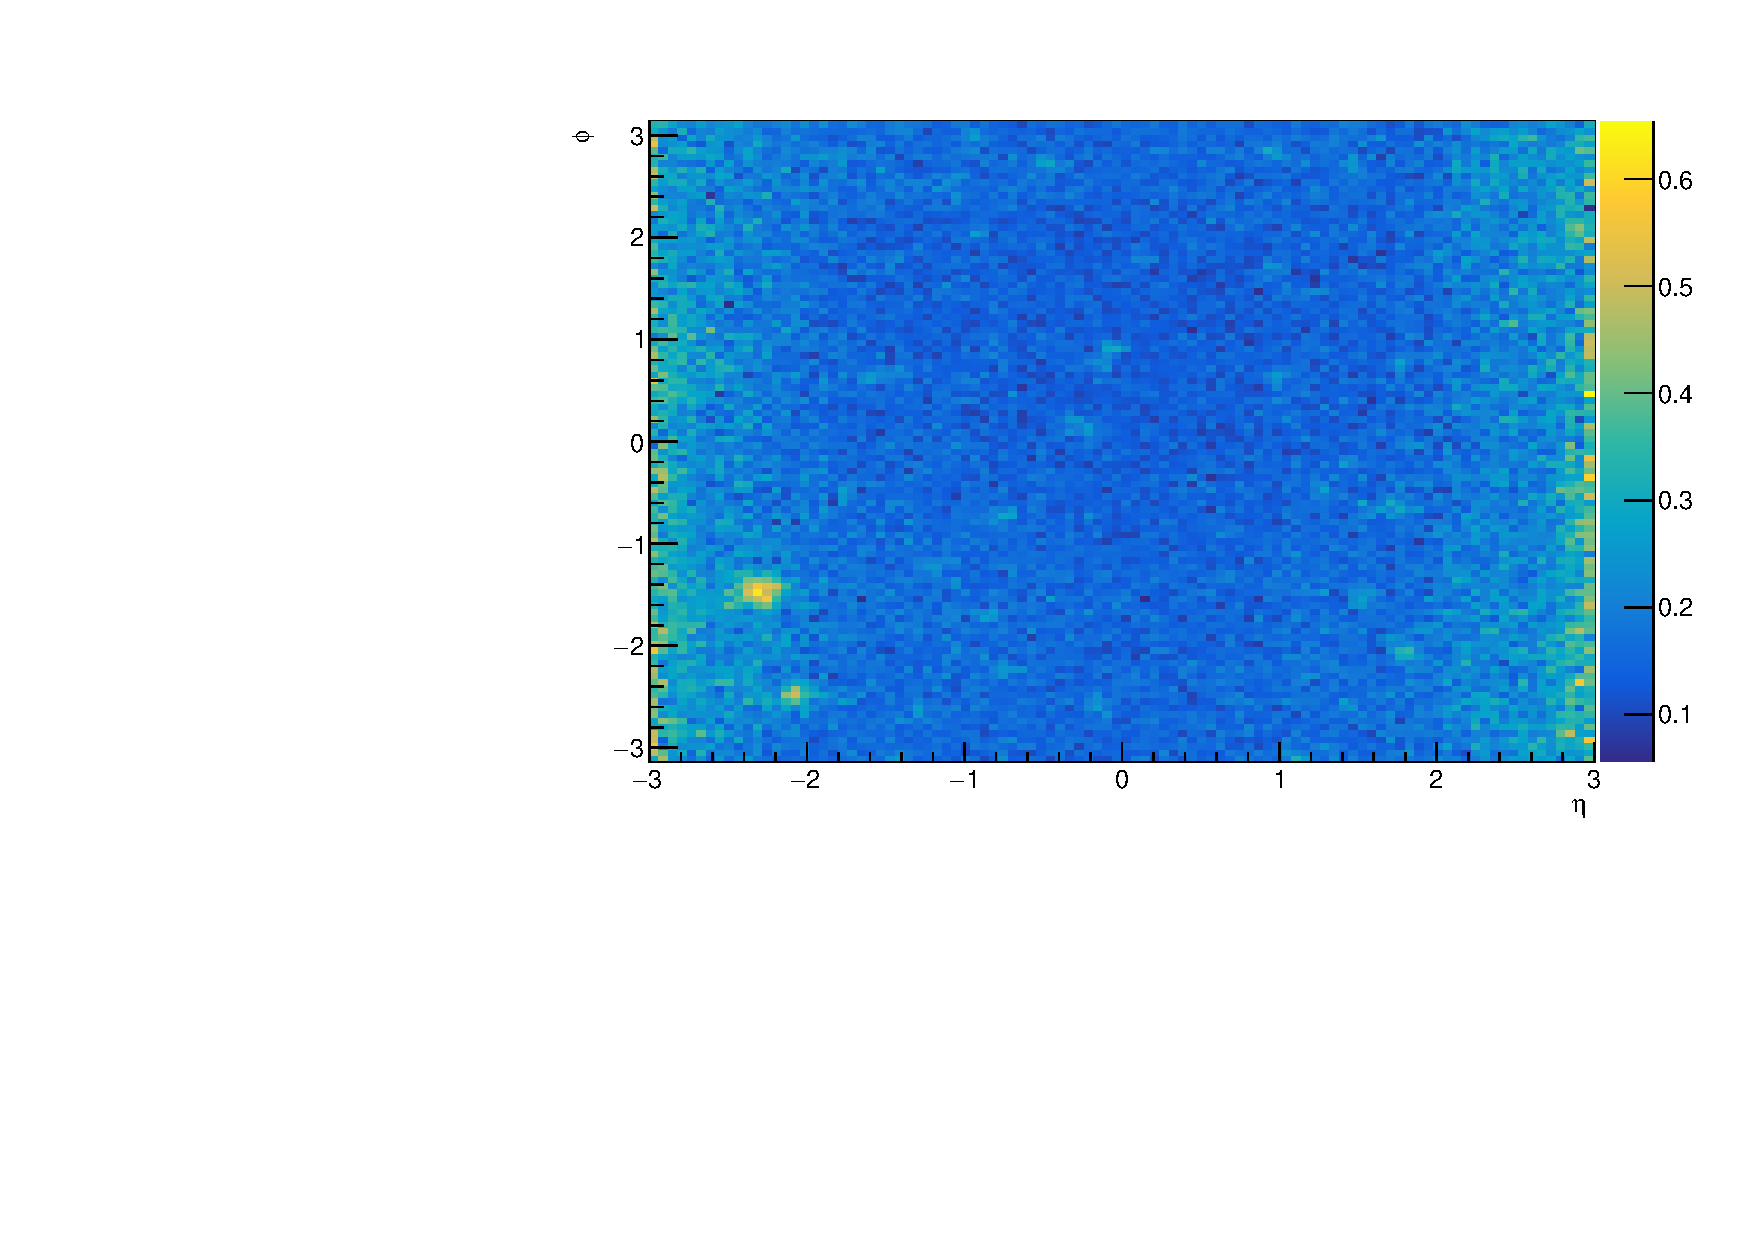
\includegraphics[width=0.7\textwidth]{figures/selection/EtaPhiMap.pdf}}
        \caption{The 2D ratio of jets ($\pt>20\gev$) with $\bdphi<0.3$ plotted in the
        $\eta-\phi$ plane, divided by all jets that satisfy $\pt>20\gev$. 
        Made with 149.49~$\text{pb}^{-1}$ of
        events that pass a loose selection of one good primary vertex,
        $\njet>1$ and $\scalht>150\gev$.}
        \label{fig:2dRatioMap}
    \end{center}
\end{figure}

\begin{figure}[h!]
    \begin{center}
        {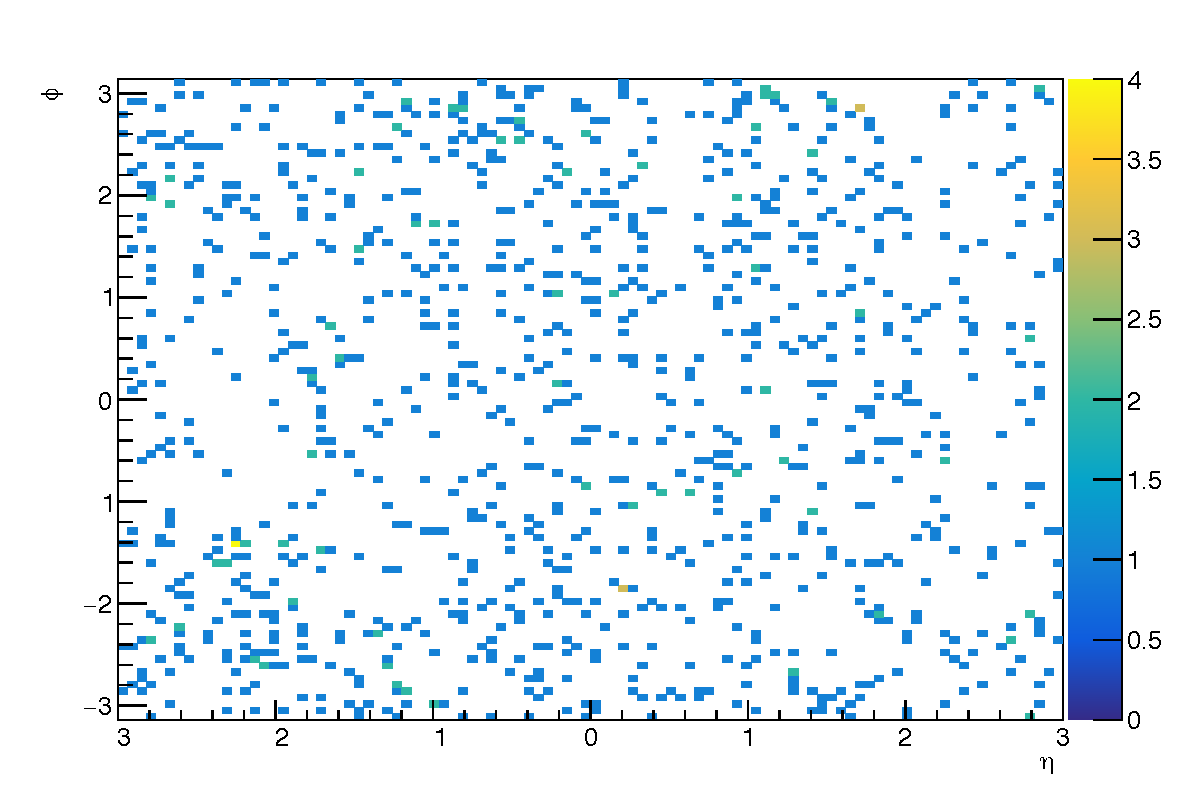
\includegraphics[width=0.7\textwidth]{figures/selection/bDPhilt0p3AfterSelection.pdf}}
        \caption{Jets ($\pt>20\gev$) with $\bdphi<0.3$ plotted in the
        $\eta-\phi$ plane. 
        Made with $1.26\ifb$ of
        events that pass the full signal region selection.}
        \label{fig:jetMapPostSignalSelection}
    \end{center}
\end{figure}

%To protect against severe energy losses caused by masked regions in the ECAL (which
%amount to about 1\% of the ECAL channel count) or HCAL, or by missing
%instrumentation in the barrel-endcap gap, events with $\bdphi < 0.5$
%are rejected if the distance in the ($\eta,\phi$) plane between the
%selected jet and the closest masked ECAL region, $\Delta R_{\rm
%  ECAL}$, is smaller than 0.3. Similarly, events are rejected if the
%jet points within 0.3 in $\eta$ of the ECAL barrel-endcap gap at
%$|\eta| = 1.5$.

{\bf Beam halo.}

The CSC beam halo filter has been found to be less efficient during the early
Run 2 data-taking period compared to the previous run.

Beam halo events manifest themselves as single energy deposits in the
calorimeters, which introduces large amounts of ``fake'' \met. This effect is
especially prominent in the signal region monojet category, particularly at
$\phi$ coordinates of 0 and $\pi$ because of the tendency of halo particles to
lie within the plane of the LHC ring. This is evident in
Fig.~\ref{fig:leadJetCleaning}.

Such spurious events are suppressed by requiring at least 10\% of the leading
jet's energy to originate from charged hadrons, $CHF>0.1$. The effectiveness of this selection
is demonstrated in Fig.~\ref{fig:leadJetCleaning}.

Beyond the filter available in the data ntuples, the JetMET POG have
provided lists of events that should fail the CSC beam halo and bad
ECAL super cluster filters. These extra events are vetoed and the
efficiency of events in the signal region (Sec.~\ref{sec:had-signal})
and single muon control region (Sec.~\ref{subsec:mucontrolSelection})
that pass this veto for each analysis bin are plotted in
Fig.~\ref{fig:cscFilterEfficiencies}. In the vast majority of bins the
extra filters are $100\%$ efficient, with a few bins with an
inefficiency at the $2-3\%$ level. This confirms that the $CHF$ cut is
already effectively removing spurious events that are present due to
beam halo effects. 

\begin{figure}[h!]
    \begin{center}
        {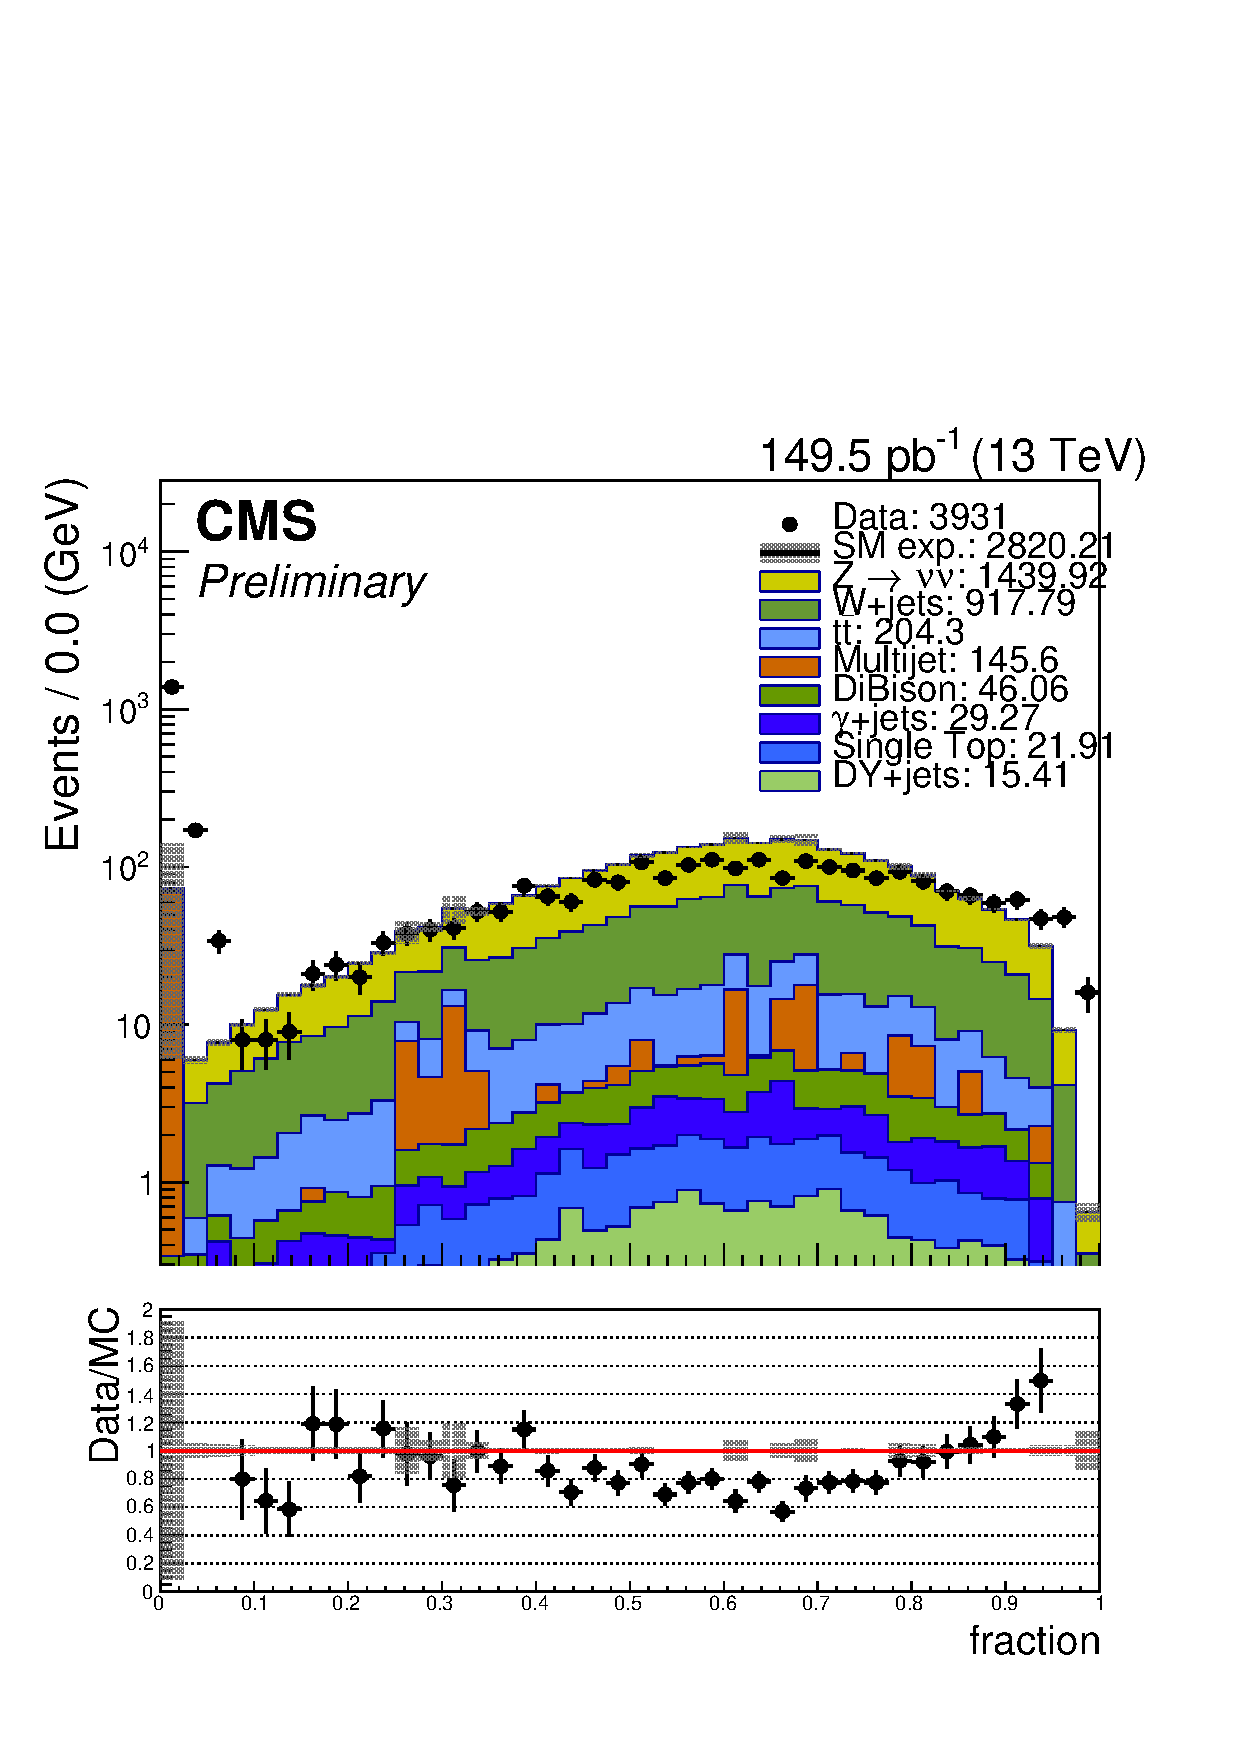
\includegraphics[width=0.32\textwidth]{figures/selection/leadJetChf_all_before.pdf}}
        {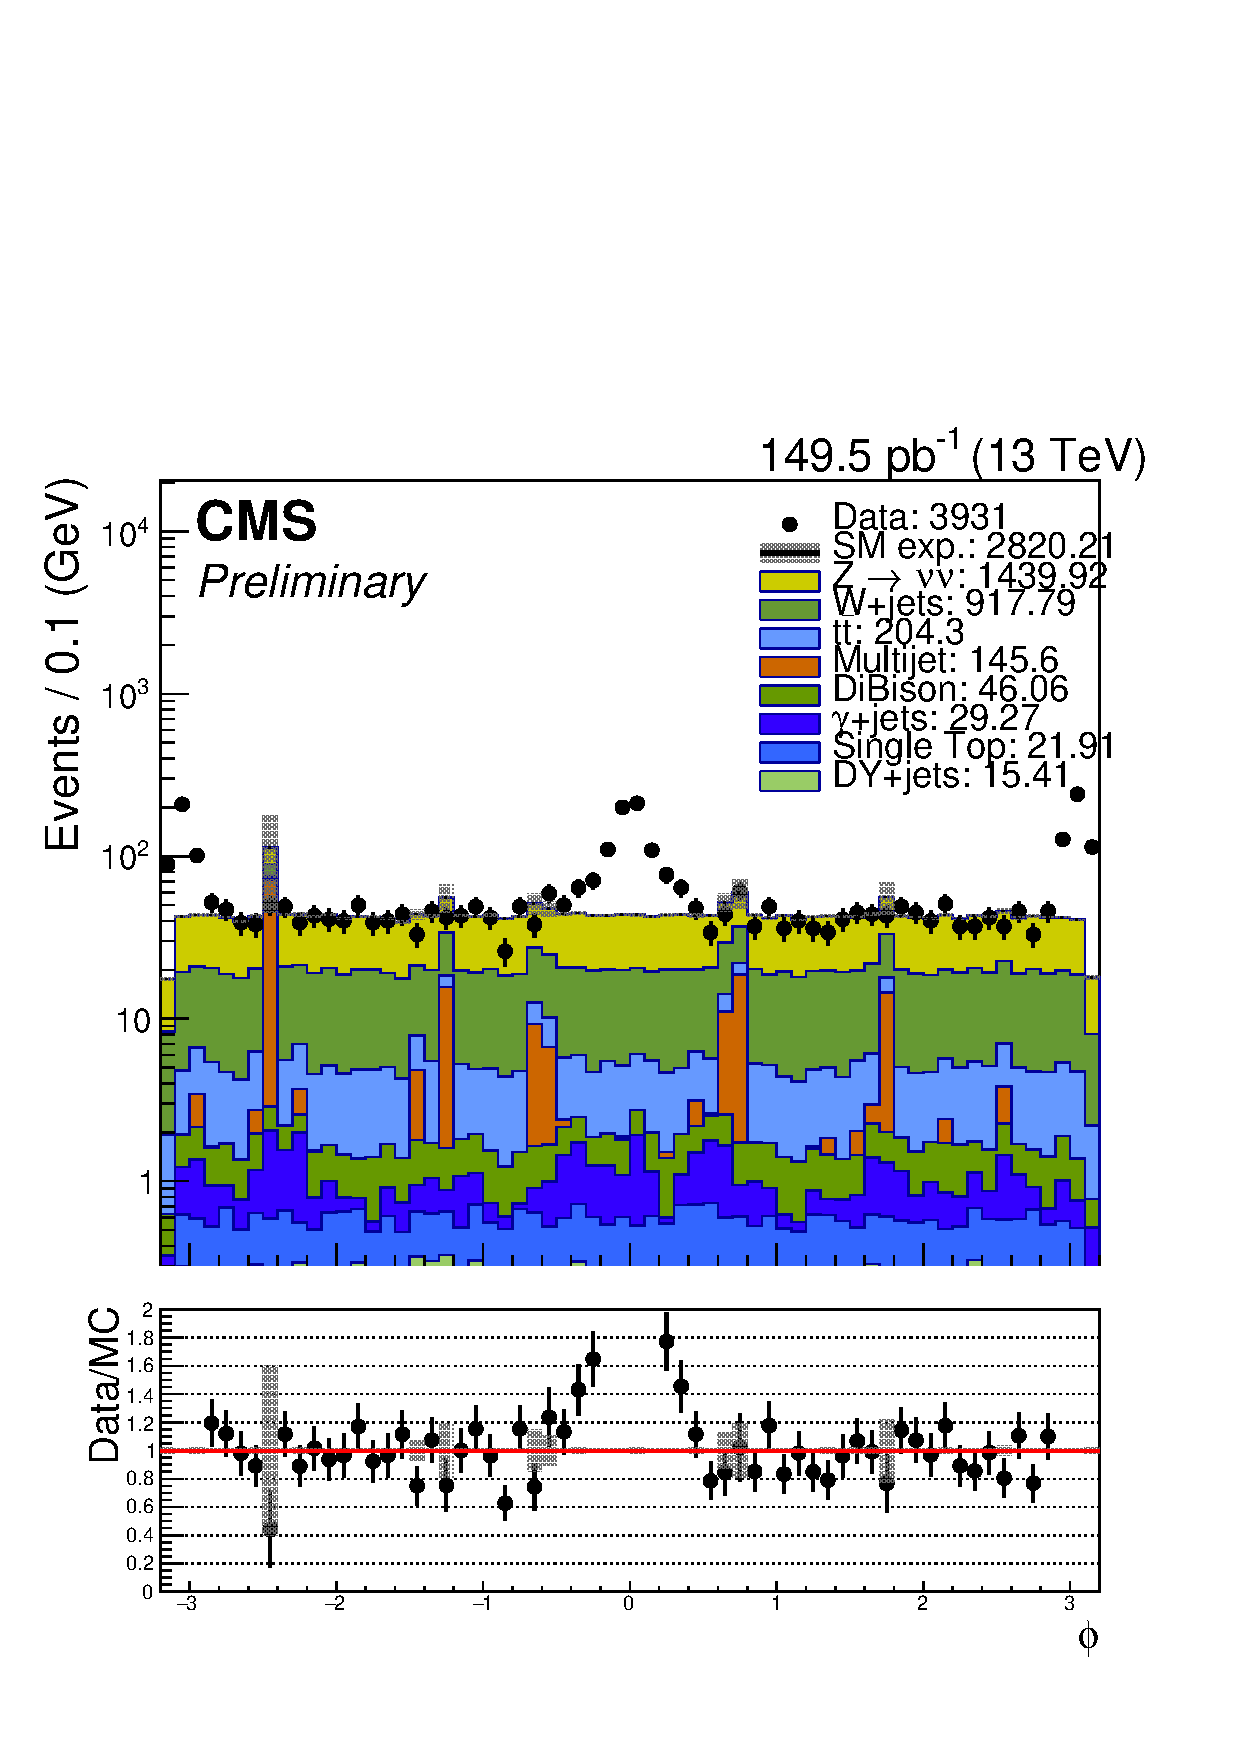
\includegraphics[width=0.32\textwidth]{figures/selection/leadJetPhi_all_before.pdf}}
        {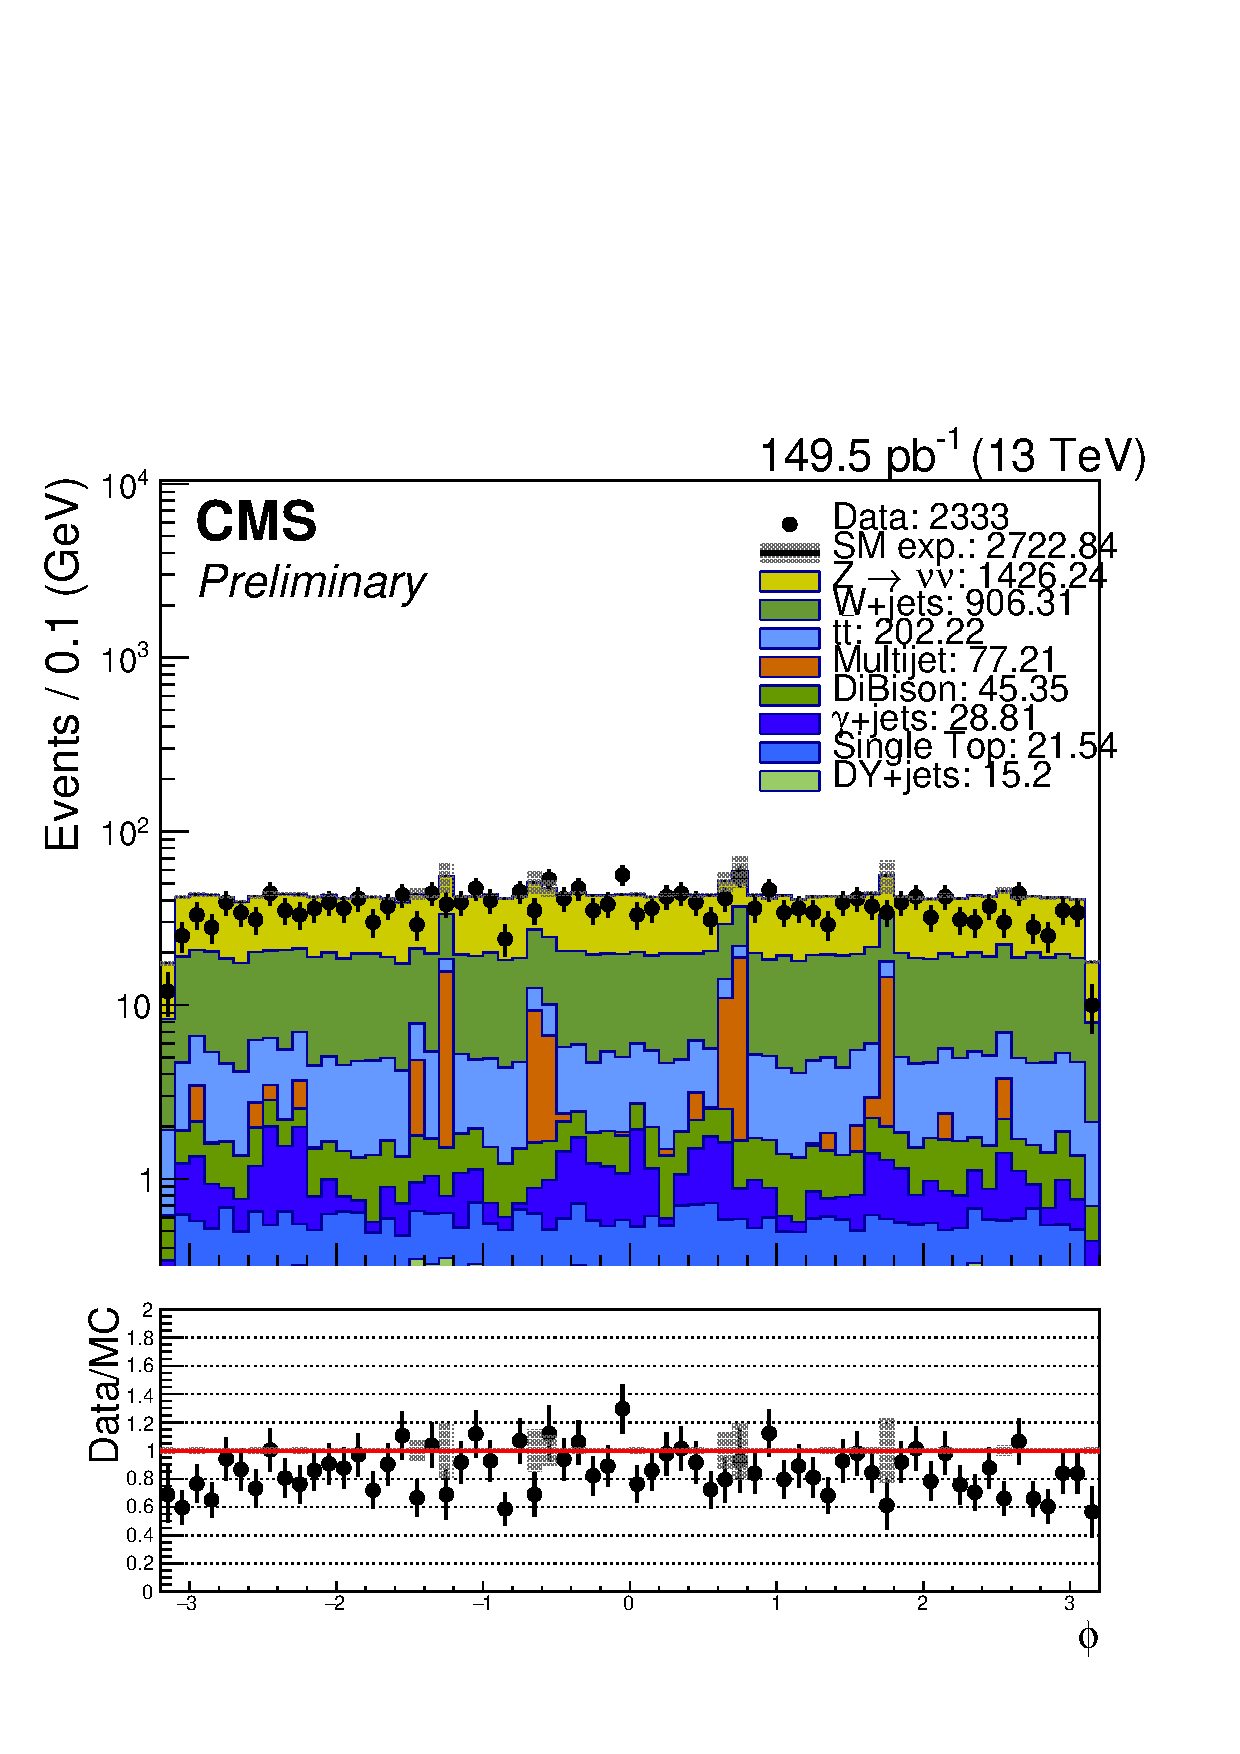
\includegraphics[width=0.32\textwidth]{figures/selection/leadJetPhi_all_after.pdf}}
        \caption{Distributions in the signal region of the lead jet charged hadron
        energy fraction (CHF) (Left), lead jet $\phi$ direction (Centre), and lead jet $\phi$
        direction after applying a requirement of {CHF~$>0.1$}. The large excess in data
        at charged hadron fractions close to zero and ${\phi = 0, \pi}$ is consistent with beam
        halo effects, and is effectively suppressed by the aforementioned selection.}
        \label{fig:leadJetCleaning}
    \end{center}
\end{figure}

\begin{figure}[h!]
  \begin{center}
    \subfigure[Signal region
    selection]{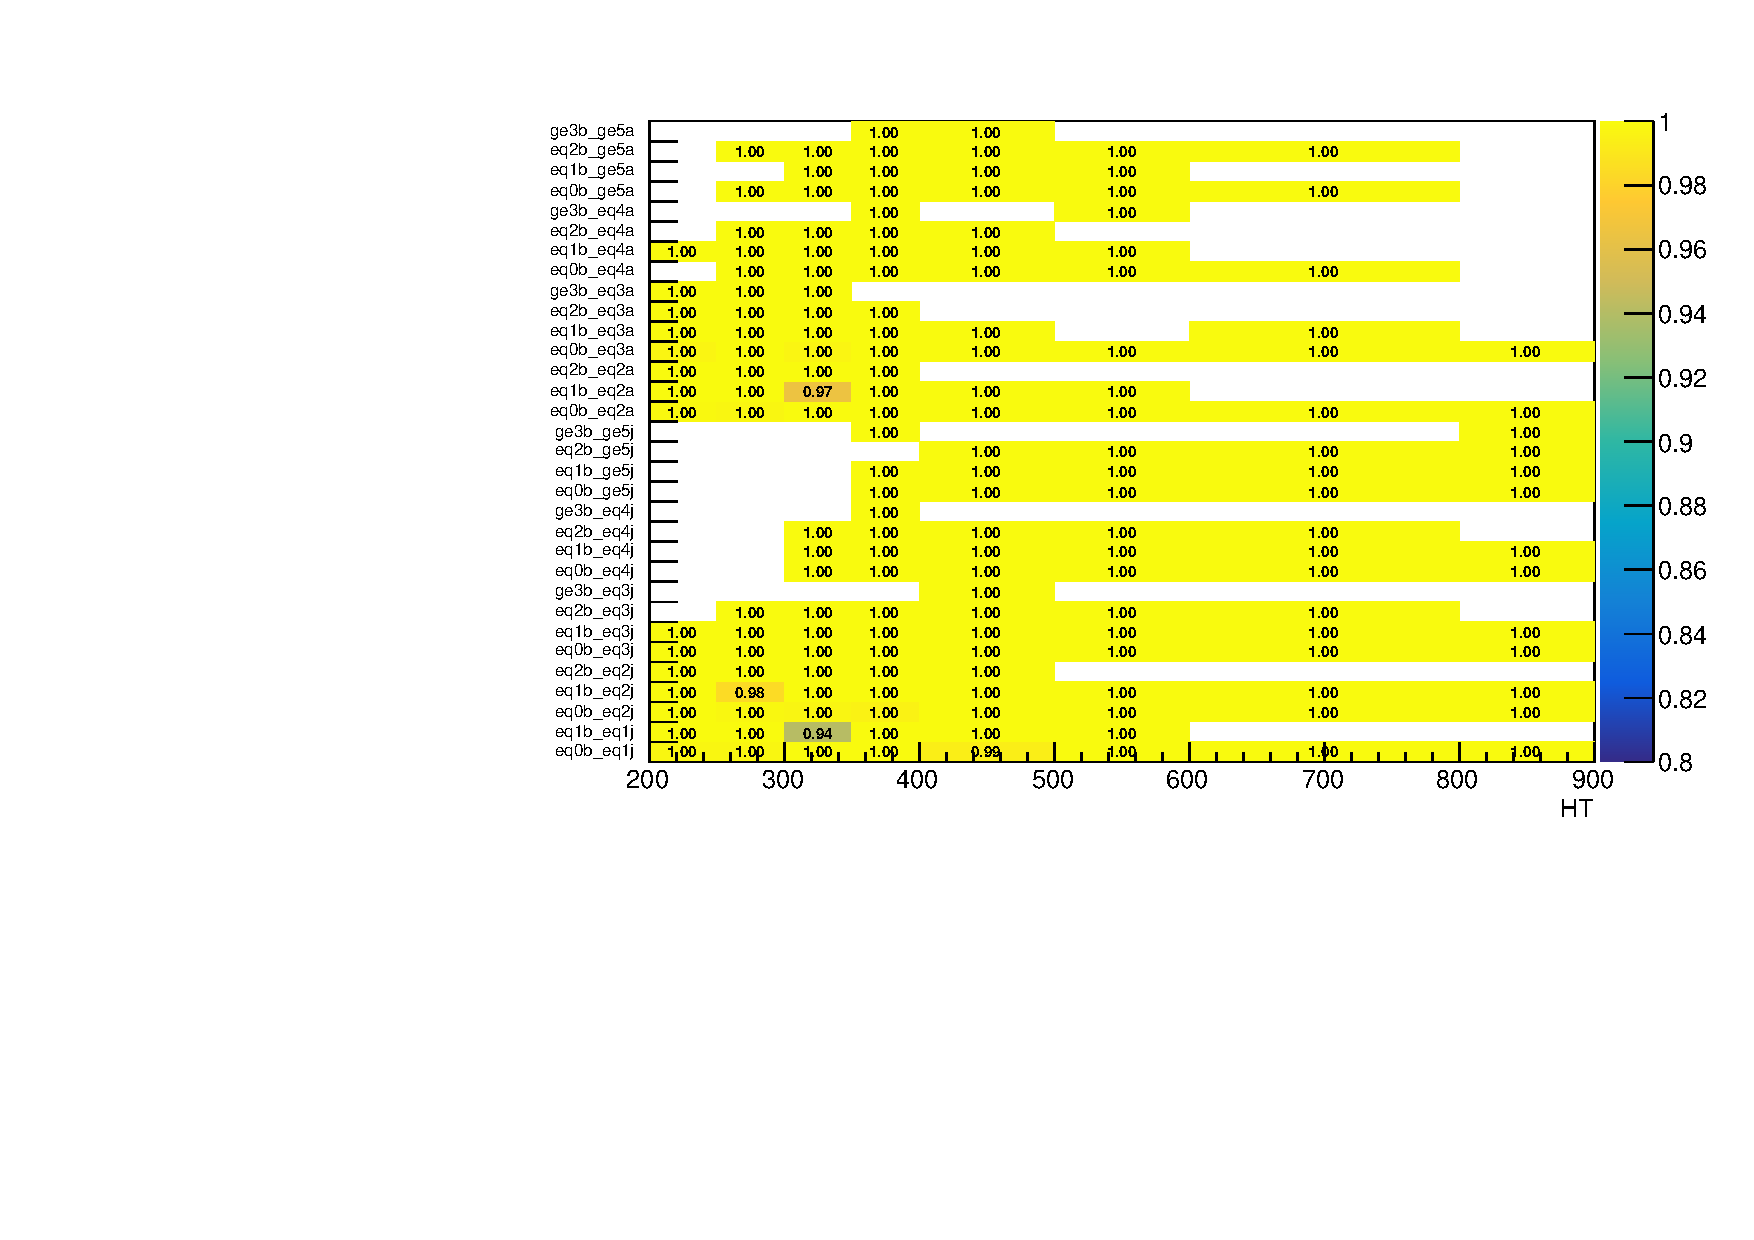
\includegraphics[width=0.5\textwidth]{figures/selection/Signal_Data_CSCEfficiency.pdf}} ~~
    \subfigure[Single muon control region
    selection]{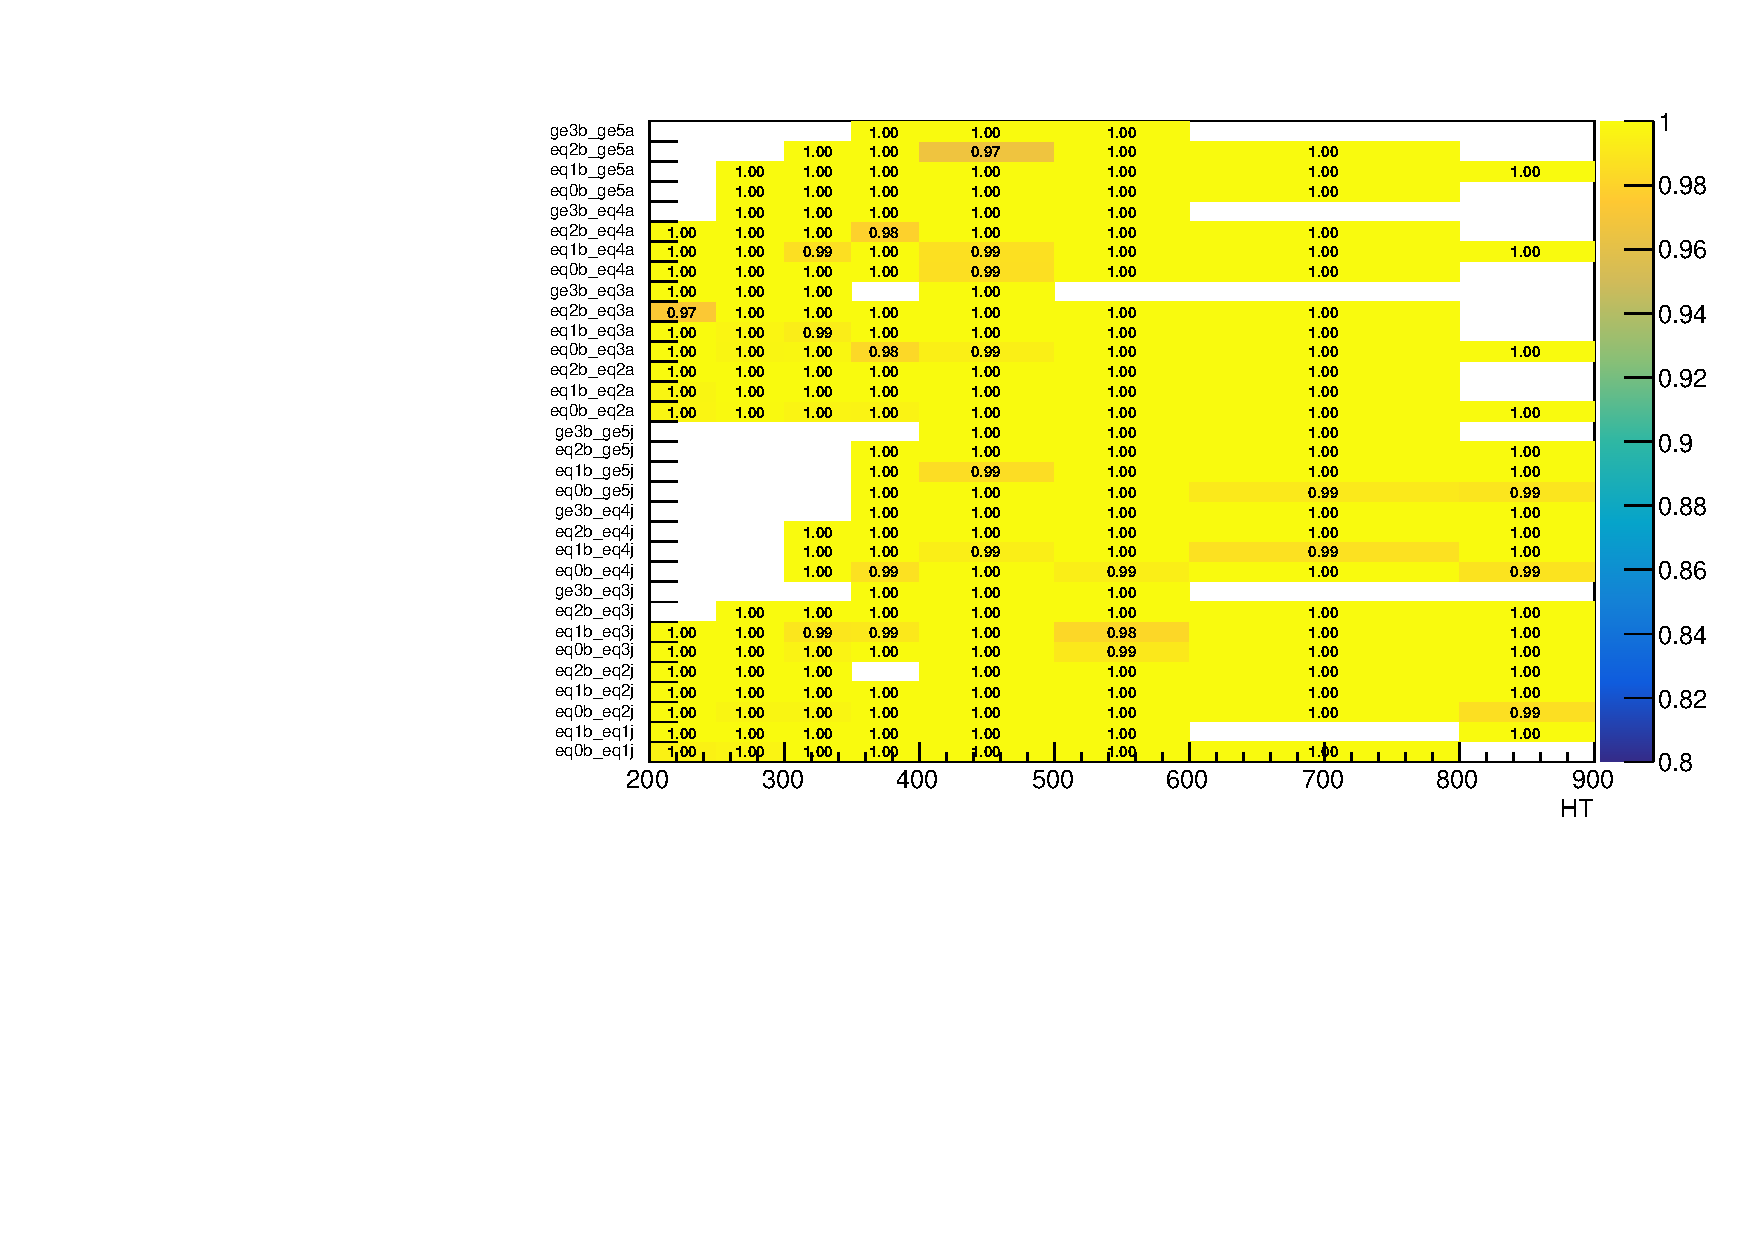
\includegraphics[width=0.5\textwidth]{figures/selection/SingleMu_Data_CSCEfficiency.pdf}} \\
    \caption{Efficiencies of the CSC beam halo and bad ECAL super
    cluster filters applied on $1.26\ifb$ of data passing the single
    muon and signal region selections.}
    \label{fig:cscFilterEfficiencies}
  \end{center} 
\end{figure}

{\bf Summary of signal region selection.} 

The requirements that define the hadronic signal region are summarised
in Table~\ref{tab:sr-selections}.

\begin{table}[h!]
  \topcaption{Summary of the signal region selection criteria, applied
    in addition to the pre-selection summarised in
    Table~\ref{tab:pre-selections}.}
  \label{tab:sr-selections}
  \centering
  \footnotesize
  \begin{tabular}{ ll }
    \hline
    \hline
    Selection             & Requirement                                                    \\
    \hline
    \alphat               & $>$0.52--0.65 (\HT-dependent) for region $200 < \HT < 800\gev$ \\
    \bdphi                & $>0.5$                                                         \\
    \mht/\met             & $<1.25$                                                        \\
    ``Dead ECAL filter''  & (see text)                                                     \\
    ``Beam Halo Filter''  &  $CHF(\textrm{leading jet})>0.1$                                \\

    \hline
    \hline
  \end{tabular}
\end{table}

\subsection{Adding the \texorpdfstring{\mht}{MHT} dimension}
\label{sec:had-shape}

As described above, and as used in Run~1, the analysis takes advantage
of three discriminating variables, \njet, \nb, and \HT, to provide
sensitivity to a large range of SUSY (and DM) models. No extrapolation
in these variables is performed, with predictions of SM background
yields in the (\njet,\nb,\HT) bins of the signal region based on both
observed counts and transfer factors derived from simulated yields in
the corresponding (\njet,\nb,\HT) bins of the control samples. Each
prediction is statistically and systematically independent.

In Run~1, for each (\njet,\nb,\HT) bin in the signal region, an
extrapolation in the variable \alphat was necessary to obtain
background predictions based on the muon control samples, which did
not impose any \alphat requirement. No extrapolation in \alphat was
performed for the photon control sample, which used the same \alphat
requirements as the signal region. The \alphat requirements used in
Run~1 for the signal region correspond loosely to \mht thresholds in
the range $\sim$130 to $\sim$500\gev depending on the \HT
bin. Uncertainties in this extrapolation were determined through
closure tests with respect to data, including one dedicated to the
\alphat extrapolation, plus additional cross checks.

In Run~2, we additionally bin event counts in the signal region
according to the variable \mht in order to provide further
discriminating power between any potential signal and the SM
background counts. Hence, while no extrapolation is performed in
\njet, \nb, nor \HT, the analysis relies on information obtained
from simulation to extrapolate from counts (integrated over \mht) in
the control samples to a predicted distribution in \mht for each
corresponding (\njet,\nb,\HT) bin in the signal region.

The \mht dimension is included in the likelihood model by using
templates determined per (\njet,\nb,\HT) bin from simulation. The
templates use an \mht bin width of 50\gev. The threshold of the final
\mht bin used by the templates is determined based on the size of the
available simulated samples: a statistical uncertainty of not more
than 50\% for the sum of all SM background processes is required. An
associated normalisation nuisance is determined from closure tests
between simulation and data, as described in
Sec.~\ref{sec:syst-on-shape}. Alternative templates are used to encode
the systematic uncertainty in the \mht distribution obtained from
simulation.

\subsection{The hadronic control region}

A hadronic control region that is enriched in multijet events and
disjoint with respect to the signal region is obtained by applying
both the pre-selection criteria and lepton/photon vetoes, as defined
above, and inverting the (\HT-dependent) \alphat and/or \mhtmet
requirements. 
%None of the cleaning filters are not applied to allow the study of
%instrumental effects. 
The sample of events populating this control region are used primarily
to estimate any residual background contamination from QCD multijet
events, described in Sec.~\ref{sec:qcd}.

\subsection{Commonalities between the data control regions}

There are five control regions with leptons or photons in the final
state: \mj, \mmj, and \gj. 
%\ej, \eej, and \gj. 
The full pre-selection is applied as part of the definition of each of these control
regions. The cuts on event-level jet-based quantities are identical to
those applied in the hadronic search region and the same \njet, \nb,
and \scalht binning is used. The lepton(s) or photon is not considered
in the calculation of the event-level variables.

The selection criteria of the various control regions are defined such
that the background composition and event kinematics of the control
regions mirror as closely as possible those for the signal
region. This is done in order to minimise the reliance on the
simulation to model correctly the backgrounds and event kinematics in
the control and signal samples.

Two exceptions are made. First, no \bdphi requirement is imposed as
part of the selection criteria defining the control regions. Second,
in the case of the four leptonic control regions, no requirement is
made on \alphat. This is made possible by the remaining kinematic
selection criteria, which are sufficiently selective to ensure that
the leptonic event samples remain rich in events from the \wj, \ttbar
and \zll processes with negligible contamination from QCD multijet
events. Thus, the acceptance of the leptonic control regions can be
significantly increased, which simultaneously improves their
predictive power and further reduces the effect of any potential
signal contamination.

The lepton event samples can be used to predict components of the SM
background across all \scalht bins, while the \gj sample can only be
used for the region $\HT > 400\gev$ due to the photon trigger
requirements.

\subsection{The \texorpdfstring{\mj}{muon plus jets} control sample}
\label{subsec:mucontrolSelection}

%Events from the \wj and \ttbar processes are found in the hadronic
%signal sample due to unidentified leptons (either out of acceptance or
%not reconstructed) and hadronic tau decays originating from
%high-p$_{T}$ W bosons. An estimate of these background processes is
%obtained through the use of a \mj sample. 

The selection criteria for the \mj sample are chosen to identify W
bosons decaying to a muon and a neutrino in the phase-space of the
signal. In order to select events containing W bosons, exactly one
tight isolated muon within an acceptance of \PT $>$ 30 \gev and
$|\eta| <$ 2.1 is required (due to the trigger), and the transverse
mass of the W candidate must satisfy $30 < \mt(\mu,\pfmet) < 125\gev$
(to suppress QCD multijet and potential signal events). Events are
vetoed if $\Delta R(\mu,\textrm{jet}_i) < 0.5$ running over all jets
$i$. The single isolated track veto, described in
Sections~\ref{sec:objects} and~\ref{sec:vetoes}, is also applied,
which considers all single isolated tracks in the event except that
associated with the identified, isolated muon. Finally, the cleaning
cut $\mht/\met$ is also applied, as done in the signal region, where
the \met is adjusted to account for the transverse momentum of the
identified, isolated muon.

\subsection{The \texorpdfstring{\mmj}{di-muon plus jets} control sample}
\label{subsec:mumucontrolSelection}

%The \znunu\ + jets process forms an irreducible background and can be
%estimated using the \zmumu + jets process, which has similar kinematic
%properties but a different acceptance and a smaller branching ratio. A
%background estimate is obtained through the use of a \mmj sample. 

The selection criteria are identical to those for the \mj sample, with
the following exceptions that are tuned to identify Z bosons decaying
to two muons in the kinematic phase space of the signal region. 
In order to select an event sample containing Z bosons, exactly two
tight isolated muons within an acceptance of $\Pt > 30\gev$ and
$|\eta| < 2.1$ are required (due to the trigger). The invariant mass
of the two muons must satisfy $m_{Z} - 25 < M_{\mu_1\mu_2} < m_{Z} +
25$ and they must have opposite charge. Events are vetoed if $\Delta
R(\mu_{i},\textrm{jet}_j) < 0.5$ is satisfied, running over all muons
$i$ and all jets $j$. The single isolated track veto is also applied
considering all single isolated tracks in the event except those
associated with the two identified, isolated muons. Finally, the
cleaning cut $\mht/\met$ is also applied, as done in the signal
region, where the \met is adjusted to account for the transverse
momenta of the two identified, isolated muons. 

% \subsection{The \texorpdfstring{\ej}{electron plus jets} control sample}
% \label{subsec:elecontrolSelection}
%
% The selection criteria that define the \ej control sample
% mirror those of the \mj sample, \ie, they are tuned
% to identify W boson decaying to an electron and a neutrino in the
% kinematic phase space of the signal region.
%
% Electrons are required to satisfy the Tight working point and satisfy
% the requirements $\Pt> 30\gev$ and $|\eta| < 2.1$. The tightening of
% the Loose working point defined in Sec.~\ref{sec:electron-id} was
% found to greatly reduce multijet contamination without a large
% reduction in statistics within the electron control samples. The
% transverse mass of the W candidate must satisfy $30 < \mt(e,\pfmet)
% < 125\gev$.
%
% \subsection{The \texorpdfstring{\eej}{electron plus jets} control sample}
% \label{subsec:dielecontrolSelection}
%
% The selection criteria that define the \eej control sample
% mirror those of the \mmj sample. They are tuned
% to identify Z boson decaying to a pair of electrons in the
% kinematic phase space of the signal region.
%
% Both electrons need to satisfy Tight working point and the
% requirements $\Pt> 30\gev$ and $|\eta| < 2.1$. The invariant mass of
% the two electrons must satisfy $m_{Z} - 25 < M_{e_1e_2} < m_{Z} + 25$
% and they must have opposite charge.

\subsection{The \texorpdfstring{\gj}{photon plus jets} control sample}
\label{subsec:photoncontrolSelection}

%The \znunu\ + jets process can also be estimated using the \gj
%process, which has a larger cross section and kinematic properties
%similar to those of \znunu\ events when the photon is
%ignored~\cite{PAS-SUS-08-002,Bern:2011pa}. 

The \gj sample is defined by requiring exactly one photon satisfying
tight isolation criteria and within an acceptance of $\pt > 200\gev$
(limited by trigger requirements) and $|\eta| < 1.45$. Furthermore,
events are vetoed if $\Delta R(\gamma,\textrm{jet}_i) < 1.0$ is
satisfied, running over all jets $i$. One important difference with
respect to the leptonic control samples is the application of the
\HT-dependent \alphat requirements imposed as part of the signal
region definition. This is done primarily to ensure that the photon
control sample and signal region are subject to identical kinematic
requirements and the photon carries sufficient transverse energy so
that the mass of the Z boson becomes a negligible effect when using
the \gj sample to predict the kinematic distributions of the \znunu
background. The cleaning cut $\mht/\met$ is also applied, as done in
the signal region, where the \met is adjusted to account for the
transverse energy of the identified, isolated photon. As stated above,
the \gj sample can only be used to predict background components in
the region $\HT > 400\gev$ due to trigger requirements.

\subsection{Control Regions}

Five control regions are defined to study modeling of important distributions and provide orthogonal selections to derive expected backgrounds in a data driven way.
These are \mj, \mmj, \gj, \eej and a hadronic control region. These control regions are designed to be kinematical close to the signal region in order to minimise the reliance on the simulation to model correctly the backgrounds and event kinematics in the control and signal samples.



The full pre-selection is applied as part of the definition of each of these control regions. The cuts on event-level jet-based quantities are identical to
those applied in the hadronic search region and the same \njet, \nb, and \scalht binning is used. The lepton(s) or photon is not considered in the calculation of the event-level variables. 

Two exceptions are made. First, no \bdphi requirement is imposed as part of the selection criteria defining the control regions. Second,
in the case of the leptonic control regions, no requirement is made on \alphat because the remaining selections ensure high purity in the \wj, \ttbar and \zll processes and only negligible  contamination from QCD multijet events. Therefore the \alphat selection has been removed to increase the statistics of the control samples selected. The lepton event samples can be used to predict components of the SM background across all \scalht bins, while the \gj sample can only be used for the region $\HT > 400\gev$ due to the photon trigger requirements. The following samples control regions are used:


\begin{itemize}

  \item{all jets} A hadronic control region that is enriched in multijet events and disjoint with respect to the signal region is obtained by applying both the pre-selection criteria and lepton/photon vetoes, as defined above, and inverting the (\HT-dependent) \alphat and/or \mhtmet requirements.  The sample of events populating this control region are used primarily to estimate any residual background contamination from QCD multijet production.

  \item{\mj} In order to select events containing W bosons, exactly one tight isolated muon within an acceptance of \PT $>$ 30 \gev and $|\eta| <$ 2.1 is required, and the transverse mass of the W candidate must satisfy $30 < \mt(\mu,\pfmet) < 125\gev$. 

  \item{\mmj} The selection criteria are identical to those for the \mj sample, while requiring two tightly isolated muons. The invariant mass of the two muons must satisfy $m_{Z} - 25 < M_{\mu_1\mu_2} < m_{Z} +25$ and they must have opposite charge.

  \item{\gj} The \gj sample is defined by requiring exactly one photon satisfying tight isolation criteria and within an acceptance of $\pt > 200\gev$ and $|\eta| < 1.45$. One important difference with respect to the leptonic control samples is the application of the \HT-dependent \alphat requirements imposed as part of the signal region definition. This is to ensure that the photon control sample and signal region are subject to identical kinematic requirements and the photon carries sufficient transverse energy so that the mass of the Z boson becomes a negligible effect when using the \gj sample to predict the kinematic distributions of the \znunu background. All cleaning requirements are applied. The \gj sample can only be used to predict background components the region $\HT > 400\gev$ due to trigger requirements.

  \item{\eej} The selection criteria that defining the \eej control sample correspond to the selection of the \mjj region

\end{itemize}



\subsection{Cross section and higher order corrections}

The cross sections for the most relevant SM background are summarised in Table~\ref{tab:cross_sections_bkg}.

\begin{table}[!h]
  \scriptsize
  \centering
  \topcaption{Cross sections for the main SM backgrounds.}
  \label{tab:cross_sections_bkg}
  \begin{tabular}
    {c|c|c|c}
    \hline\hline
    \textbf{Sample} & \textbf{Cross section (pb)} & \textbf{Accuracy} & \textbf{K-factor} \\
    \hline
    W+jets, $100 < \scalht < 200$ GeV & $1347 \pm 2$ & LO & 1.21 \\
    W+jets, $200 < \scalht < 400$ GeV & $360 \pm 1$ & LO & 1.21 \\
    W+jets, $400 < \scalht < 600$ GeV & $48.9 \pm 0.17$ & LO & 1.21 \\
    W+jets, $600 < \scalht < 800$ GeV & $12.8 \pm 0.4$ & LO & 1.21 \\
    W+jets, $800 < \scalht < 1200$ GeV & $5.26 \pm 0.19$ & LO & 1.21 \\
    W+jets, $1200 < \scalht < 2500$ GeV & $1.33 \pm 0.05$ & LO & 1.21 \\
    W+jets, $\scalht > 2500$ GeV & $0.0309 \pm 0.0011$ & LO & 1.21 \\
    \hline
    DY+jets, $100 < \scalht < 200$ GeV & $139 \pm 4$ & LO & 1.23 \\
    DY+jets, $200 < \scalht < 400$ GeV & $42.8 \pm 1.4$ & LO & 1.23 \\
    DY+jets, $400 < \scalht < 600$ GeV & $5.5 \pm 0.2$ & LO & 1.23 \\
    DY+jets, $\scalht > 600$ GeV & $2.2 \pm 0.8$ & LO & 1.23 \\
    \hline
    $\gamma$+jets, $40 < \scalht < 100$ GeV & $20730 \pm 66$ & LO & - \\
    $\gamma$+jets, $100 < \scalht < 200$ GeV & $9226 \pm 36$ & LO & - \\
    $\gamma$+jets, $200 < \scalht < 400$ GeV & $2281 \pm 47$ & LO & - \\
    $\gamma$+jets, $400 < \scalht < 600$ GeV & $273 \pm 9$ & LO & - \\
    $\gamma$+jets, $\scalht > 600$ GeV & $94.5 \pm 3.2$ & LO & - \\
    \hline
    $Z\rightarrow \nu\nu$+jets, $100 < \scalht < 200$ GeV & $280.47$ & LO & 1.23 \\
    $Z\rightarrow \nu\nu$+jets, $200 < \scalht < 400$ GeV & $78.36$ & LO & 1.23 \\
    $Z\rightarrow \nu\nu$+jets, $400 < \scalht < 600$ GeV & $10.94$ & LO & 1.23 \\
    $Z\rightarrow \nu\nu$+jets, $\scalht > 600$ GeV & $4.20$ & LO & 1.23 \\
    \hline
    TTJets & $831.76^{+20}_{-30}$ & NNLO & - \\
    \hline \hline
  \end{tabular}
\end{table}


The cross sections are known only to a limited number of perturbative orders and additional corrections might be sizeable. 
If available NLO corrections (K-factors) are applied. These come either from theoretical calculations if available or enriched sidebands for the relevant process. 
Furthermore the analysis strategy is such that there is little dependence to the normalization of simulated samples. Backgrounds normalisations are estimated
from control regions in data, and the effect of cross section corrections on the transfer factors is expected to largely cancel out because of the similar background composition 
between signal and the control regions. However, we want to avoid large extrapolations where possible. Therefore we
measure in data residual cross section corrections to the background processes using sidebands enriched in a single process. This allows to apply these data driven separately and to compare where available the correction with available K-factors. We briefly list here the list of sidebands and resulting corrections. Details and control plots can be found again in ~\cite{alphaTnote}.

\begin{itemize}

  \item{\gj} The \gj sample is available only in LO accuracy and in contrast to all other samples no k-factor is available. As shown in Sec. 8 of \citee{alphaTnote} the expected yield from simulations differs from the expectation by about 20\%.  For $\ht < 400$ GeV, events are selected in the interval $0.50 < \alphat < 0.52$, and for $\ht>400$~GeV $ 0.50 <\alphat < 0.53$. The data yields are corrected for remaining QCD contaminations taken from simulations and the correction is determined.

  \item{$V$+jets and \ttbar production} 
 For the $V$+jets and \ttj samples the cross section are at known at NLO, NNLL accuracy respectively. The corrections for $V$+jets are about 1.2
 We define a sideband by inverting \htmiss selection to $100<\htmiss<130$ and cross checked using the  $\htmiss/\etmiss > 1.25$ region. Both results are found to be compatible within the statistical
 uncertainties. To increase purity the following additional selections are applied: For $W$+jets production we require one muon in the final state, not more than 2 jets and no identified $b$-jets. For $Z$+jets we require exactly two muons and no $b$-jets.  Finally to enrich \ttj production one muon, two light- and two $b$-jets are required.

\end{itemiez}




\section{Expected yields and distributions in the signal region}

In the absence of multijet events from QCD, the remaining significant backgrounds in the signal region are expected to stem from SM
processes with genuine \met in the final state. For the low jet multiplicity categories, the largest backgrounds with genuine \met are
from the associated production of W or Z bosons with jets, followed by either the weak decays \znunu\ or \wtaunu, where the $\tau$ decays
hadronically and is identified as a jet, or by leptonic decays that are outside acceptance or not rejected by the dedicated electron or
muon vetoes. For the higher jet multiplicity categories, top quark production followed by semileptonic weak top quark decay becomes
dominant. The relative contribution from \ttbar depends on the jet multiplicity with increase importance for large jet multiplicities.

Tables~\ref{tab:prednodata_sig_comb_sym},
\ref{tab:prednodata_sig_comb_asym} and \ref{tab:prednodata_sig_comb_mono} 
summarise the predicted pre-fit yields and uncertainties in the signal region for an integrated
luminosity of 1.28 \ifb. In addition to the total expected yield (SM) per (\njet,~\nb,~\scalht) bin, the $\ttbar$W and \znunu\ contributions
are also shown (the former of which contains all residual contributions from sub-dominant processes such as \eg diboson
production).
\clearpage
\begin{table}[h!]
\tiny
\centering
\caption{Pre fit Yields in the signal region for 2.1\ifb for symmetric categories. All entries are non-zero but are truncated to one decimal place.\label{tab:prednodata_sig_comb_sym}}
\begin{tabular}
{cccccccccc}
	\hline\hline
	&	& \multicolumn{8}{c}{\scalht (\gev)}\\ 
	&	 (\njet, \nb) & 200-250 & 250-300 & 300-350 & 350-400 & 400-500 & 500-600 & 600-800 & 800-$\infty$ \\ [0.8ex] 
\hline
	SM & (2, 0) & $943.9^{+ 134.2 }_{- 134.2 }$ & $938.4^{+ 148.4 }_{- 148.4 }$ & $627.9^{+ 86.0 }_{- 86.0 }$ & $341.4^{+ 61.3 }_{- 61.3 }$ & $329.1^{+ 38.4 }_{- 38.4 }$ & $105.2^{+ 24.3 }_{- 24.3 }$ & $43.8^{+ 12.2 }_{- 12.2 }$ & $44.4^{+ 11.4 }_{- 11.4 }$ \\[0.5ex] 
	Ttw & (2, 0) & $425.8^{+ 84.5 }_{- 84.5 }$ & $415.9^{+ 81.1 }_{- 81.1 }$ & $262.5^{+ 41.1 }_{- 41.1 }$ & $128.7^{+ 24.8 }_{- 24.8 }$ & $113.1^{+ 12.9 }_{- 12.9 }$ & $33.0^{+ 9.1 }_{- 9.1 }$ & $13.3^{+ 2.7 }_{- 2.7 }$ & $12.8^{+ 2.8 }_{- 2.8 }$ \\[0.5ex] 
	Zinv & (2, 0) & $457.5^{+ 86.4 }_{- 86.4 }$ & $517.5^{+ 116.8 }_{- 116.8 }$ & $353.5^{+ 63.8 }_{- 63.8 }$ & $210.4^{+ 50.0 }_{- 50.0 }$ & $206.4^{+ 28.1 }_{- 28.1 }$ & $67.7^{+ 18.5 }_{- 18.5 }$ & $30.4^{+ 11.0 }_{- 11.0 }$ & $31.2^{+ 9.5 }_{- 9.5 }$ \\[0.5ex] 
	SM & (2, 1) & $80.9^{+ 16.0 }_{- 16.0 }$ & $57.9^{+ 11.1 }_{- 11.1 }$ & $40.8^{+ 7.3 }_{- 7.3 }$ & $26.8^{+ 5.7 }_{- 5.7 }$ & $24.1^{+ 3.7 }_{- 3.7 }$ & $9.5^{+ 2.7 }_{- 2.7 }$ & $4.0^{+ 1.4 }_{- 1.4 }$ & $3.7^{+ 1.3 }_{- 1.3 }$ \\[0.5ex] 
	Ttw & (2, 1) & $50.5^{+ 12.8 }_{- 12.8 }$ & $33.7^{+ 7.4 }_{- 7.4 }$ & $20.3^{+ 4.2 }_{- 4.2 }$ & $11.0^{+ 2.6 }_{- 2.6 }$ & $8.4^{+ 1.3 }_{- 1.3 }$ & $2.9^{+ 1.0 }_{- 1.0 }$ & $1.0^{+ 0.3 }_{- 0.3 }$ & $1.0^{+ 0.3 }_{- 0.3 }$ \\[0.5ex] 
	Zinv & (2, 1) & $25.2^{+ 6.0 }_{- 6.0 }$ & $23.9^{+ 5.9 }_{- 5.9 }$ & $19.8^{+ 4.3 }_{- 4.3 }$ & $15.7^{+ 4.0 }_{- 4.0 }$ & $14.9^{+ 2.5 }_{- 2.5 }$ & $6.2^{+ 2.0 }_{- 2.0 }$ & $3.0^{+ 1.2 }_{- 1.2 }$ & $2.6^{+ 1.0 }_{- 1.0 }$ \\[0.5ex] 
	SM & (2, 2) & $1.1^{+ 2.3 }_{- 2.3 }$ & $0.8^{+ 1.9 }_{- 1.9 }$ & $3.4^{+ 2.0 }_{- 2.0 }$ & $0.7^{+ 0.8 }_{- 0.8 }$ & $1.1^{+ 0.5 }_{- 0.5 }$ & $1.3^{+ 0.8 }_{- 0.8 }$ & $0.2^{+ 0.2 }_{- 0.2 }$ & -- \\[0.5ex] 
	Ttw & (2, 2) & $0.5^{+ 1.2 }_{- 1.2 }$ & $0.4^{+ 0.9 }_{- 0.9 }$ & $1.7^{+ 1.0 }_{- 1.0 }$ & $0.3^{+ 0.3 }_{- 0.3 }$ & $0.4^{+ 0.2 }_{- 0.2 }$ & $0.8^{+ 0.6 }_{- 0.6 }$ & $0.1^{+ 0.0 }_{- 0.0 }$ & -- \\[0.5ex] 
	Zinv & (2, 2) & $0.5^{+ 1.1 }_{- 1.1 }$ & $0.4^{+ 1.0 }_{- 1.0 }$ & $1.6^{+ 1.0 }_{- 1.0 }$ & $0.4^{+ 0.4 }_{- 0.4 }$ & $0.6^{+ 0.3 }_{- 0.3 }$ & $0.4^{+ 0.2 }_{- 0.2 }$ & $0.1^{+ 0.1 }_{- 0.1 }$ & -- \\[0.5ex] 
	SM & (3, 0) & $0.0^{+ 2.4 }_{- 2.4 }$ & $173.6^{+ 26.2 }_{- 26.2 }$ & $491.8^{+ 63.6 }_{- 63.6 }$ & $421.9^{+ 58.6 }_{- 58.6 }$ & $499.2^{+ 65.1 }_{- 65.1 }$ & $195.4^{+ 36.8 }_{- 36.8 }$ & $89.5^{+ 23.7 }_{- 23.7 }$ & $68.0^{+ 11.6 }_{- 11.6 }$ \\[0.5ex] 
	Ttw & (3, 0) & $0.0^{+ 1.9 }_{- 1.9 }$ & $80.3^{+ 12.6 }_{- 12.6 }$ & $237.0^{+ 35.4 }_{- 35.4 }$ & $190.6^{+ 27.4 }_{- 27.4 }$ & $207.0^{+ 32.1 }_{- 32.1 }$ & $68.1^{+ 14.1 }_{- 14.1 }$ & $29.1^{+ 5.3 }_{- 5.3 }$ & $18.1^{+ 3.6 }_{- 3.6 }$ \\[0.5ex] 
	Zinv & (3, 0) & $0.0^{+ 0.6 }_{- 0.6 }$ & $90.9^{+ 19.9 }_{- 19.9 }$ & $243.3^{+ 47.7 }_{- 47.7 }$ & $212.9^{+ 38.9 }_{- 38.9 }$ & $282.4^{+ 44.2 }_{- 44.2 }$ & $111.6^{+ 25.2 }_{- 25.2 }$ & $60.4^{+ 21.2 }_{- 21.2 }$ & $45.4^{+ 8.8 }_{- 8.8 }$ \\[0.5ex] 
	SM & (3, 1) & -- & $37.9^{+ 6.3 }_{- 6.3 }$ & $70.5^{+ 11.1 }_{- 11.1 }$ & $81.2^{+ 11.9 }_{- 11.9 }$ & $79.2^{+ 11.6 }_{- 11.6 }$ & $26.4^{+ 5.9 }_{- 5.9 }$ & $15.3^{+ 4.1 }_{- 4.1 }$ & $9.2^{+ 2.0 }_{- 2.0 }$ \\[0.5ex] 
	Ttw & (3, 1) & -- & $29.3^{+ 5.2 }_{- 5.2 }$ & $51.3^{+ 9.6 }_{- 9.6 }$ & $54.3^{+ 8.1 }_{- 8.1 }$ & $47.4^{+ 7.9 }_{- 7.9 }$ & $13.0^{+ 3.3 }_{- 3.3 }$ & $5.9^{+ 1.2 }_{- 1.2 }$ & $2.7^{+ 0.7 }_{- 0.7 }$ \\[0.5ex] 
	Zinv & (3, 1) & -- & $8.1^{+ 2.0 }_{- 2.0 }$ & $17.6^{+ 3.7 }_{- 3.7 }$ & $23.4^{+ 5.1 }_{- 5.1 }$ & $30.2^{+ 5.6 }_{- 5.6 }$ & $11.2^{+ 3.0 }_{- 3.0 }$ & $9.4^{+ 3.5 }_{- 3.5 }$ & $5.9^{+ 1.5 }_{- 1.5 }$ \\[0.5ex] 
	SM & (3, 2) & -- & $5.9^{+ 1.7 }_{- 1.7 }$ & $17.5^{+ 3.2 }_{- 3.2 }$ & $16.4^{+ 3.0 }_{- 3.0 }$ & $11.3^{+ 2.2 }_{- 2.2 }$ & $3.4^{+ 1.0 }_{- 1.0 }$ & $0.8^{+ 0.3 }_{- 0.3 }$ & $0.9^{+ 0.3 }_{- 0.3 }$ \\[0.5ex] 
	Ttw & (3, 2) & -- & $4.7^{+ 1.4 }_{- 1.4 }$ & $14.3^{+ 2.8 }_{- 2.8 }$ & $13.5^{+ 2.7 }_{- 2.7 }$ & $8.5^{+ 1.8 }_{- 1.8 }$ & $2.0^{+ 0.6 }_{- 0.6 }$ & $0.2^{+ 0.1 }_{- 0.1 }$ & $0.3^{+ 0.1 }_{- 0.1 }$ \\[0.5ex] 
	Zinv & (3, 2) & -- & $1.2^{+ 0.4 }_{- 0.4 }$ & $2.8^{+ 0.6 }_{- 0.6 }$ & $2.2^{+ 0.5 }_{- 0.5 }$ & $2.7^{+ 0.6 }_{- 0.6 }$ & $1.1^{+ 0.4 }_{- 0.4 }$ & $0.5^{+ 0.2 }_{- 0.2 }$ & $0.6^{+ 0.2 }_{- 0.2 }$ \\[0.5ex] 
	SM & (3, $\ge3$) & -- & $0.0^{+ 0.3 }_{- 0.3 }$ & -- & -- & $0.4^{+ 0.2 }_{- 0.2 }$ & -- & -- & -- \\[0.5ex] 
	Ttw & (3, $\ge3$) & -- & $0.0^{+ 0.3 }_{- 0.3 }$ & -- & -- & $0.3^{+ 0.2 }_{- 0.2 }$ & -- & -- & -- \\[0.5ex] 
	Zinv & (3, $\ge3$) & -- & $0.0^{+ 0.0 }_{- 0.0 }$ & -- & -- & $0.1^{+ 0.0 }_{- 0.0 }$ & -- & -- & -- \\[0.5ex] 
	SM & (4, 0) & -- & -- & $48.8^{+ 14.1 }_{- 14.1 }$ & $163.1^{+ 65.7 }_{- 65.7 }$ & $301.0^{+ 46.9 }_{- 46.9 }$ & $155.8^{+ 36.3 }_{- 36.3 }$ & $96.5^{+ 19.1 }_{- 19.1 }$ & $52.8^{+ 11.3 }_{- 11.3 }$ \\[0.5ex] 
	Ttw & (4, 0) & -- & -- & $27.7^{+ 10.0 }_{- 10.0 }$ & $87.3^{+ 27.6 }_{- 27.6 }$ & $150.8^{+ 19.9 }_{- 19.9 }$ & $62.9^{+ 15.6 }_{- 15.6 }$ & $35.4^{+ 7.6 }_{- 7.6 }$ & $17.3^{+ 4.5 }_{- 4.5 }$ \\[0.5ex] 
	Zinv & (4, 0) & -- & -- & $20.6^{+ 8.0 }_{- 8.0 }$ & $74.8^{+ 54.5 }_{- 54.5 }$ & $150.2^{+ 36.3 }_{- 36.3 }$ & $88.5^{+ 27.6 }_{- 27.6 }$ & $60.7^{+ 13.5 }_{- 13.5 }$ & $35.5^{+ 8.3 }_{- 8.3 }$ \\[0.5ex] 
	SM & (4, 1) & -- & -- & $19.9^{+ 6.3 }_{- 6.3 }$ & $67.1^{+ 19.0 }_{- 19.0 }$ & $84.6^{+ 11.7 }_{- 11.7 }$ & $36.9^{+ 8.3 }_{- 8.3 }$ & $18.4^{+ 4.3 }_{- 4.3 }$ & $11.6^{+ 2.5 }_{- 2.5 }$ \\[0.5ex] 
	Ttw & (4, 1) & -- & -- & $17.0^{+ 6.0 }_{- 6.0 }$ & $55.4^{+ 16.3 }_{- 16.3 }$ & $65.5^{+ 9.0 }_{- 9.0 }$ & $23.4^{+ 6.0 }_{- 6.0 }$ & $9.9^{+ 2.6 }_{- 2.6 }$ & $4.7^{+ 1.2 }_{- 1.2 }$ \\[0.5ex] 
	Zinv & (4, 1) & -- & -- & $2.7^{+ 1.1 }_{- 1.1 }$ & $11.3^{+ 8.9 }_{- 8.9 }$ & $19.0^{+ 4.9 }_{- 4.9 }$ & $12.5^{+ 3.7 }_{- 3.7 }$ & $8.5^{+ 2.1 }_{- 2.1 }$ & $6.9^{+ 1.6 }_{- 1.6 }$ \\[0.5ex] 
	SM & (4, 2) & -- & -- & $3.6^{+ 2.0 }_{- 2.0 }$ & $17.2^{+ 5.8 }_{- 5.8 }$ & $31.9^{+ 5.0 }_{- 5.0 }$ & $7.3^{+ 2.1 }_{- 2.1 }$ & $2.8^{+ 0.7 }_{- 0.7 }$ & $2.1^{+ 0.6 }_{- 0.6 }$ \\[0.5ex] 
	Ttw & (4, 2) & -- & -- & $3.2^{+ 1.9 }_{- 1.9 }$ & $16.2^{+ 5.7 }_{- 5.7 }$ & $28.5^{+ 4.6 }_{- 4.6 }$ & $5.9^{+ 1.8 }_{- 1.8 }$ & $1.7^{+ 0.4 }_{- 0.4 }$ & $1.1^{+ 0.4 }_{- 0.4 }$ \\[0.5ex] 
	Zinv & (4, 2) & -- & -- & $0.4^{+ 0.2 }_{- 0.2 }$ & $0.9^{+ 0.6 }_{- 0.6 }$ & $3.4^{+ 0.9 }_{- 0.9 }$ & $1.2^{+ 0.4 }_{- 0.4 }$ & $1.0^{+ 0.3 }_{- 0.3 }$ & $1.0^{+ 0.3 }_{- 0.3 }$ \\[0.5ex] 
	SM & (4, $\ge3$) & -- & -- & $0.0^{+ 0.4 }_{- 0.4 }$ & $1.5^{+ 1.1 }_{- 1.1 }$ & $1.5^{+ 0.8 }_{- 0.8 }$ & $0.6^{+ 0.4 }_{- 0.4 }$ & $0.0^{+ 0.1 }_{- 0.1 }$ & $0.0^{+ 0.0 }_{- 0.0 }$ \\[0.5ex] 
	Ttw & (4, $\ge3$) & -- & -- & $0.0^{+ 0.4 }_{- 0.4 }$ & $1.3^{+ 1.0 }_{- 1.0 }$ & $1.4^{+ 0.7 }_{- 0.7 }$ & $0.5^{+ 0.3 }_{- 0.3 }$ & $0.0^{+ 0.0 }_{- 0.0 }$ & $0.0^{+ 0.0 }_{- 0.0 }$ \\[0.5ex] 
	Zinv & (4, $\ge3$) & -- & -- & $0.0^{+ 0.0 }_{- 0.0 }$ & $0.1^{+ 0.2 }_{- 0.2 }$ & $0.1^{+ 0.1 }_{- 0.1 }$ & $0.1^{+ 0.1 }_{- 0.1 }$ & $0.0^{+ 0.0 }_{- 0.0 }$ & $0.0^{+ 0.0 }_{- 0.0 }$ \\[0.5ex] 
	SM & ($\ge5$, 0) & -- & -- & -- & $15.3^{+ 5.9 }_{- 5.9 }$ & $86.1^{+ 13.1 }_{- 13.1 }$ & $78.1^{+ 20.0 }_{- 20.0 }$ & $71.0^{+ 14.4 }_{- 14.4 }$ & $46.2^{+ 12.8 }_{- 12.8 }$ \\[0.5ex] 
	Ttw & ($\ge5$, 0) & -- & -- & -- & $10.5^{+ 4.9 }_{- 4.9 }$ & $49.9^{+ 8.9 }_{- 8.9 }$ & $37.3^{+ 9.8 }_{- 9.8 }$ & $32.4^{+ 6.9 }_{- 6.9 }$ & $17.0^{+ 4.1 }_{- 4.1 }$ \\[0.5ex] 
	Zinv & ($\ge5$, 0) & -- & -- & -- & $4.7^{+ 1.4 }_{- 1.4 }$ & $32.8^{+ 7.5 }_{- 7.5 }$ & $36.1^{+ 11.8 }_{- 11.8 }$ & $37.4^{+ 9.6 }_{- 9.6 }$ & $28.1^{+ 10.4 }_{- 10.4 }$ \\[0.5ex] 
	SM & ($\ge5$, 1) & -- & -- & -- & $2.5^{+ 1.5 }_{- 1.5 }$ & $44.1^{+ 8.0 }_{- 8.0 }$ & $38.9^{+ 8.7 }_{- 8.7 }$ & $25.3^{+ 5.6 }_{- 5.6 }$ & $15.8^{+ 3.5 }_{- 3.5 }$ \\[0.5ex] 
	Ttw & ($\ge5$, 1) & -- & -- & -- & $2.2^{+ 1.4 }_{- 1.4 }$ & $37.4^{+ 7.4 }_{- 7.4 }$ & $30.8^{+ 7.3 }_{- 7.3 }$ & $18.5^{+ 4.6 }_{- 4.6 }$ & $9.9^{+ 2.3 }_{- 2.3 }$ \\[0.5ex] 
	Zinv & ($\ge5$, 1) & -- & -- & -- & $0.3^{+ 0.1 }_{- 0.1 }$ & $5.0^{+ 1.3 }_{- 1.3 }$ & $5.8^{+ 2.0 }_{- 2.0 }$ & $6.3^{+ 1.7 }_{- 1.7 }$ & $5.6^{+ 1.9 }_{- 1.9 }$ \\[0.5ex] 
	SM & ($\ge5$, 2) & -- & -- & -- & $2.1^{+ 1.3 }_{- 1.3 }$ & $18.8^{+ 4.1 }_{- 4.1 }$ & $15.4^{+ 3.8 }_{- 3.8 }$ & $7.6^{+ 1.9 }_{- 1.9 }$ & $4.6^{+ 1.2 }_{- 1.2 }$ \\[0.5ex] 
	Ttw & ($\ge5$, 2) & -- & -- & -- & $2.0^{+ 1.3 }_{- 1.3 }$ & $17.3^{+ 4.0 }_{- 4.0 }$ & $13.2^{+ 3.5 }_{- 3.5 }$ & $6.4^{+ 1.7 }_{- 1.7 }$ & $3.6^{+ 1.0 }_{- 1.0 }$ \\[0.5ex] 
	Zinv & ($\ge5$, 2) & -- & -- & -- & $0.1^{+ 0.1 }_{- 0.1 }$ & $0.8^{+ 0.3 }_{- 0.3 }$ & $1.3^{+ 0.5 }_{- 0.5 }$ & $1.1^{+ 0.3 }_{- 0.3 }$ & $0.9^{+ 0.4 }_{- 0.4 }$ \\[0.5ex] 
	SM & ($\ge5$, $\ge3$) & -- & -- & -- & -- & $0.7^{+ 0.7 }_{- 0.7 }$ & $1.2^{+ 0.7 }_{- 0.7 }$ & $1.4^{+ 0.5 }_{- 0.5 }$ & $0.8^{+ 0.3 }_{- 0.3 }$ \\[0.5ex] 
	Ttw & ($\ge5$, $\ge3$) & -- & -- & -- & -- & $0.7^{+ 0.7 }_{- 0.7 }$ & $1.1^{+ 0.7 }_{- 0.7 }$ & $1.1^{+ 0.4 }_{- 0.4 }$ & $0.6^{+ 0.2 }_{- 0.2 }$ \\[0.5ex] 
	Zinv & ($\ge5$, $\ge3$) & -- & -- & -- & -- & $0.0^{+ 0.0 }_{- 0.0 }$ & $0.0^{+ 0.0 }_{- 0.0 }$ & $0.2^{+ 0.1 }_{- 0.1 }$ & $0.2^{+ 0.1 }_{- 0.1 }$ \\[0.5ex] 
	\hline
	\hline
\end{tabular}
\end{table}

\clearpage
\begin{table}[h!]
\tiny
\centering
\caption{Predictions and Data in the signal region for 1.26\ifb for asymmetric categories. The letter ``a'' in jet \eg ``2a''  indicates the asymmetric jet bins. All entries are non-zero but are truncated to one decimal place.\label{tab:prednodata_sig_comb_asym}}
\begin{tabular}
{cccccccccc}
	\hline\hline
&	&	& \multicolumn{8}{c}{\scalht (\gev)}\\ 
	&	 (\njet, \nb) & 200-250 & 250-300 & 300-350 & 350-400 & 400-500 & 500-600 & 600-800 & 800-$\infty$ \\ [0.8ex] 
\hline
	SM & (2a, 0) & $2811.3^{+ 309.8 }_{- 309.7 }$ & $795.9^{+ 102.0 }_{- 101.9 }$ & $291.8^{+ 48.3 }_{- 48.3 }$ & $117.9^{+ 19.2 }_{- 19.1 }$ & $90.8^{+ 18.2 }_{- 18.2 }$ & $20.6^{+ 5.9 }_{- 5.9 }$ & $5.3^{+ 3.4 }_{- 3.4 }$ & -- \\[0.5ex] 
	Ttw & (2a, 0) & $1319.3^{+ 185.1 }_{- 185.0 }$ & $333.0^{+ 54.3 }_{- 54.3 }$ & $115.1^{+ 26.1 }_{- 26.1 }$ & $40.9^{+ 8.6 }_{- 8.6 }$ & $27.5^{+ 6.0 }_{- 6.0 }$ & $6.3^{+ 2.0 }_{- 2.0 }$ & $1.3^{+ 2.6 }_{- 2.6 }$ & -- \\[0.5ex] 
	Zinv & (2a, 0) & $1492.0^{+ 191.1 }_{- 191.0 }$ & $462.9^{+ 74.0 }_{- 74.0 }$ & $176.8^{+ 31.1 }_{- 31.0 }$ & $77.0^{+ 13.7 }_{- 13.6 }$ & $63.3^{+ 14.4 }_{- 14.4 }$ & $14.3^{+ 4.8 }_{- 4.7 }$ & $4.0^{+ 2.1 }_{- 2.1 }$ & -- \\[0.5ex] 
	SM & (2a, 1) & $217.2^{+ 26.0 }_{- 25.9 }$ & $82.6^{+ 11.5 }_{- 11.4 }$ & $22.3^{+ 4.3 }_{- 4.2 }$ & $10.5^{+ 2.3 }_{- 2.1 }$ & $6.4^{+ 1.6 }_{- 1.5 }$ & $1.5^{+ 0.7 }_{- 0.6 }$ & $0.3^{+ 0.3 }_{- 0.2 }$ & -- \\[0.5ex] 
	Ttw & (2a, 1) & $133.4^{+ 19.9 }_{- 19.8 }$ & $45.6^{+ 8.2 }_{- 8.2 }$ & $10.6^{+ 2.8 }_{- 2.8 }$ & $3.6^{+ 1.1 }_{- 1.0 }$ & $2.3^{+ 0.8 }_{- 0.8 }$ & $0.4^{+ 0.3 }_{- 0.3 }$ & $0.1^{+ 0.2 }_{- 0.2 }$ & -- \\[0.5ex] 
	Zinv & (2a, 1) & $83.8^{+ 11.6 }_{- 11.5 }$ & $37.0^{+ 6.5 }_{- 6.4 }$ & $11.8^{+ 2.5 }_{- 2.4 }$ & $6.9^{+ 1.8 }_{- 1.6 }$ & $4.0^{+ 1.2 }_{- 1.2 }$ & $1.1^{+ 0.6 }_{- 0.5 }$ & $0.2^{+ 0.2 }_{- 0.1 }$ & -- \\[0.5ex] 
	SM & (2a, 2) & $13.3^{+ 2.5 }_{- 2.3 }$ & $2.7^{+ 0.8 }_{- 0.7 }$ & $2.5^{+ 0.9 }_{- 0.8 }$ & $1.6^{+ 0.8 }_{- 0.7 }$ & $0.8^{+ 0.4 }_{- 0.4 }$ & $0.1^{+ 0.1 }_{- 0.1 }$ & $0.1^{+ 0.1 }_{- 0.1 }$ & -- \\[0.5ex] 
	Ttw & (2a, 2) & $7.2^{+ 1.8 }_{- 1.7 }$ & $1.4^{+ 0.6 }_{- 0.5 }$ & $1.3^{+ 0.7 }_{- 0.6 }$ & $1.1^{+ 0.8 }_{- 0.7 }$ & $0.3^{+ 0.3 }_{- 0.2 }$ & $0.0^{+ 0.0 }_{- 0.0 }$ & $0.0^{+ 0.1 }_{- 0.1 }$ & -- \\[0.5ex] 
	Zinv & (2a, 2) & $6.1^{+ 1.5 }_{- 1.3 }$ & $1.3^{+ 0.5 }_{- 0.4 }$ & $1.3^{+ 0.6 }_{- 0.5 }$ & $0.4^{+ 0.3 }_{- 0.2 }$ & $0.4^{+ 0.3 }_{- 0.2 }$ & $0.1^{+ 0.1 }_{- 0.1 }$ & $0.0^{+ 0.1 }_{- 0.0 }$ & -- \\[0.5ex] 
	SM & (3a, 0) & $720.3^{+ 104.8 }_{- 104.6 }$ & $718.0^{+ 77.6 }_{- 77.5 }$ & $364.1^{+ 69.8 }_{- 69.7 }$ & $126.8^{+ 26.6 }_{- 26.5 }$ & $58.6^{+ 12.9 }_{- 12.9 }$ & $10.9^{+ 4.0 }_{- 3.9 }$ & $3.3^{+ 2.2 }_{- 2.1 }$ & -- \\[0.5ex] 
	Ttw & (3a, 0) & $377.0^{+ 67.8 }_{- 67.7 }$ & $364.5^{+ 48.3 }_{- 48.2 }$ & $178.2^{+ 42.2 }_{- 42.1 }$ & $53.0^{+ 14.7 }_{- 14.6 }$ & $21.3^{+ 6.2 }_{- 6.2 }$ & $3.5^{+ 1.5 }_{- 1.5 }$ & $0.8^{+ 0.7 }_{- 0.7 }$ & -- \\[0.5ex] 
	Zinv & (3a, 0) & $343.3^{+ 68.7 }_{- 68.6 }$ & $353.4^{+ 45.3 }_{- 45.2 }$ & $185.9^{+ 44.5 }_{- 44.4 }$ & $73.8^{+ 19.0 }_{- 18.9 }$ & $37.3^{+ 9.4 }_{- 9.3 }$ & $7.3^{+ 3.3 }_{- 3.3 }$ & $2.5^{+ 2.0 }_{- 2.0 }$ & -- \\[0.5ex] 
	SM & (3a, 1) & $127.2^{+ 20.7 }_{- 20.6 }$ & $143.8^{+ 17.6 }_{- 17.5 }$ & $53.9^{+ 11.4 }_{- 11.3 }$ & $16.6^{+ 4.0 }_{- 3.9 }$ & $7.6^{+ 1.9 }_{- 1.9 }$ & $1.2^{+ 0.5 }_{- 0.5 }$ & $0.4^{+ 0.3 }_{- 0.3 }$ & -- \\[0.5ex] 
	Ttw & (3a, 1) & $102.7^{+ 19.2 }_{- 19.1 }$ & $113.2^{+ 15.7 }_{- 15.6 }$ & $40.4^{+ 10.0 }_{- 9.9 }$ & $11.1^{+ 3.4 }_{- 3.3 }$ & $4.2^{+ 1.4 }_{- 1.4 }$ & $0.7^{+ 0.4 }_{- 0.4 }$ & $0.1^{+ 0.1 }_{- 0.1 }$ & -- \\[0.5ex] 
	Zinv & (3a, 1) & $24.5^{+ 5.1 }_{- 5.1 }$ & $30.6^{+ 4.2 }_{- 4.2 }$ & $13.5^{+ 3.4 }_{- 3.4 }$ & $5.5^{+ 1.6 }_{- 1.6 }$ & $3.5^{+ 1.0 }_{- 1.0 }$ & $0.5^{+ 0.3 }_{- 0.2 }$ & $0.3^{+ 0.3 }_{- 0.3 }$ & -- \\[0.5ex] 
	SM & (3a, 2) & $23.9^{+ 4.6 }_{- 4.5 }$ & $22.1^{+ 3.4 }_{- 3.3 }$ & $14.2^{+ 3.6 }_{- 3.5 }$ & $5.0^{+ 1.6 }_{- 1.5 }$ & $1.2^{+ 0.4 }_{- 0.4 }$ & $0.2^{+ 0.2 }_{- 0.1 }$ & $0.0^{+ 0.1 }_{- 0.0 }$ & -- \\[0.5ex] 
	Ttw & (3a, 2) & $20.5^{+ 4.4 }_{- 4.3 }$ & $18.5^{+ 3.2 }_{- 3.1 }$ & $11.9^{+ 3.4 }_{- 3.3 }$ & $4.3^{+ 1.5 }_{- 1.4 }$ & $0.7^{+ 0.3 }_{- 0.3 }$ & $0.1^{+ 0.1 }_{- 0.1 }$ & $0.0^{+ 0.0 }_{- 0.0 }$ & -- \\[0.5ex] 
	Zinv & (3a, 2) & $3.4^{+ 0.9 }_{- 0.8 }$ & $3.6^{+ 0.7 }_{- 0.7 }$ & $2.3^{+ 0.7 }_{- 0.7 }$ & $0.7^{+ 0.3 }_{- 0.3 }$ & $0.5^{+ 0.2 }_{- 0.2 }$ & $0.1^{+ 0.1 }_{- 0.1 }$ & $0.0^{+ 0.1 }_{- 0.0 }$ & -- \\[0.5ex] 
	SM & (3a, $\ge3$) & $0.2^{+ 0.3 }_{- 0.1 }$ & $0.7^{+ 0.4 }_{- 0.3 }$ & $0.4^{+ 0.4 }_{- 0.2 }$ & -- & $0.0^{+ 0.0 }_{- 0.0 }$ & -- & -- & -- \\[0.5ex] 
	Ttw & (3a, $\ge3$) & $0.2^{+ 0.3 }_{- 0.1 }$ & $0.6^{+ 0.4 }_{- 0.3 }$ & $0.4^{+ 0.4 }_{- 0.2 }$ & -- & $0.0^{+ 0.0 }_{- 0.0 }$ & -- & -- & -- \\[0.5ex] 
	Zinv & (3a, $\ge3$) & $0.0^{+ 0.0 }_{- 0.0 }$ & $0.1^{+ 0.1 }_{- 0.1 }$ & $0.0^{+ 0.0 }_{- 0.0 }$ & -- & $0.0^{+ 0.0 }_{- 0.0 }$ & -- & -- & -- \\[0.5ex] 
	SM & (4a, 0) & $1.7^{+ 0.8 }_{- 0.7 }$ & $72.6^{+ 24.1 }_{- 24.1 }$ & $167.8^{+ 30.4 }_{- 30.2 }$ & $111.8^{+ 19.6 }_{- 19.4 }$ & $61.9^{+ 14.5 }_{- 14.4 }$ & $7.6^{+ 2.1 }_{- 2.1 }$ & $1.2^{+ 0.7 }_{- 0.6 }$ & -- \\[0.5ex] 
	Ttw & (4a, 0) & $0.6^{+ 0.4 }_{- 0.4 }$ & $41.6^{+ 15.1 }_{- 15.0 }$ & $91.8^{+ 20.5 }_{- 20.3 }$ & $61.2^{+ 13.4 }_{- 13.2 }$ & $28.7^{+ 9.5 }_{- 9.4 }$ & $2.8^{+ 1.1 }_{- 1.0 }$ & $0.3^{+ 0.2 }_{- 0.2 }$ & -- \\[0.5ex] 
	Zinv & (4a, 0) & $1.1^{+ 0.7 }_{- 0.6 }$ & $31.0^{+ 18.4 }_{- 18.4 }$ & $76.0^{+ 16.4 }_{- 16.2 }$ & $50.6^{+ 10.0 }_{- 9.9 }$ & $33.3^{+ 8.5 }_{- 8.4 }$ & $4.8^{+ 1.5 }_{- 1.4 }$ & $0.9^{+ 0.6 }_{- 0.6 }$ & -- \\[0.5ex] 
	SM & (4a, 1) & $0.6^{+ 0.3 }_{- 0.3 }$ & $15.6^{+ 5.1 }_{- 5.0 }$ & $63.4^{+ 13.1 }_{- 13.0 }$ & $39.2^{+ 7.9 }_{- 7.8 }$ & $27.0^{+ 7.6 }_{- 7.5 }$ & $1.7^{+ 0.6 }_{- 0.6 }$ & $0.3^{+ 0.2 }_{- 0.2 }$ & -- \\[0.5ex] 
	Ttw & (4a, 1) & $0.4^{+ 0.3 }_{- 0.2 }$ & $12.5^{+ 4.7 }_{- 4.6 }$ & $54.4^{+ 12.3 }_{- 12.2 }$ & $32.6^{+ 7.3 }_{- 7.2 }$ & $20.4^{+ 6.9 }_{- 6.8 }$ & $1.1^{+ 0.5 }_{- 0.5 }$ & $0.1^{+ 0.1 }_{- 0.1 }$ & -- \\[0.5ex] 
	Zinv & (4a, 1) & $0.1^{+ 0.1 }_{- 0.1 }$ & $3.1^{+ 1.9 }_{- 1.9 }$ & $9.0^{+ 2.0 }_{- 2.0 }$ & $6.7^{+ 1.4 }_{- 1.4 }$ & $6.6^{+ 1.8 }_{- 1.8 }$ & $0.7^{+ 0.3 }_{- 0.3 }$ & $0.2^{+ 0.1 }_{- 0.1 }$ & -- \\[0.5ex] 
	SM & (4a, 2) & $0.2^{+ 0.2 }_{- 0.1 }$ & $6.1^{+ 2.2 }_{- 2.1 }$ & $21.8^{+ 5.2 }_{- 5.0 }$ & $15.8^{+ 3.8 }_{- 3.6 }$ & $6.4^{+ 2.2 }_{- 2.1 }$ & $0.3^{+ 0.2 }_{- 0.2 }$ & $0.1^{+ 0.1 }_{- 0.1 }$ & -- \\[0.5ex] 
	Ttw & (4a, 2) & $0.2^{+ 0.2 }_{- 0.1 }$ & $5.2^{+ 2.1 }_{- 2.0 }$ & $20.3^{+ 5.0 }_{- 4.9 }$ & $14.9^{+ 3.7 }_{- 3.6 }$ & $5.7^{+ 2.2 }_{- 2.1 }$ & $0.3^{+ 0.2 }_{- 0.2 }$ & $0.1^{+ 0.1 }_{- 0.1 }$ & -- \\[0.5ex] 
	Zinv & (4a, 2) & $0.0^{+ 0.0 }_{- 0.0 }$ & $0.9^{+ 0.6 }_{- 0.6 }$ & $1.5^{+ 0.4 }_{- 0.4 }$ & $0.9^{+ 0.3 }_{- 0.3 }$ & $0.7^{+ 0.3 }_{- 0.3 }$ & $0.1^{+ 0.1 }_{- 0.0 }$ & $0.0^{+ 0.0 }_{- 0.0 }$ & -- \\[0.5ex] 
	SM & (4a, $\ge3$) & -- & $0.5^{+ 0.5 }_{- 0.3 }$ & $1.3^{+ 0.9 }_{- 0.6 }$ & $0.7^{+ 0.5 }_{- 0.3 }$ & $0.9^{+ 0.7 }_{- 0.5 }$ & $0.1^{+ 0.2 }_{- 0.1 }$ & -- & -- \\[0.5ex] 
	Ttw & (4a, $\ge3$) & -- & $0.4^{+ 0.5 }_{- 0.3 }$ & $1.2^{+ 0.9 }_{- 0.6 }$ & $0.7^{+ 0.5 }_{- 0.3 }$ & $0.9^{+ 0.7 }_{- 0.5 }$ & $0.1^{+ 0.2 }_{- 0.1 }$ & -- & -- \\[0.5ex] 
	Zinv & (4a, $\ge3$) & -- & $0.0^{+ 0.0 }_{- 0.0 }$ & $0.1^{+ 0.1 }_{- 0.1 }$ & $0.0^{+ 0.1 }_{- 0.0 }$ & $0.0^{+ 0.0 }_{- 0.0 }$ & $0.0^{+ 0.0 }_{- 0.0 }$ & -- & -- \\[0.5ex] 
	SM & ($\ge5$a, 0) & -- & -- & $11.3^{+ 4.1 }_{- 3.6 }$ & $38.7^{+ 9.0 }_{- 8.6 }$ & $51.9^{+ 13.0 }_{- 12.9 }$ & $8.2^{+ 2.9 }_{- 2.8 }$ & $2.6^{+ 1.5 }_{- 1.4 }$ & -- \\[0.5ex] 
	Ttw & ($\ge5$a, 0) & -- & -- & $7.1^{+ 3.3 }_{- 2.8 }$ & $24.2^{+ 6.9 }_{- 6.5 }$ & $33.2^{+ 9.3 }_{- 9.2 }$ & $4.5^{+ 2.2 }_{- 2.1 }$ & $1.2^{+ 0.8 }_{- 0.7 }$ & -- \\[0.5ex] 
	Zinv & ($\ge5$a, 0) & -- & -- & $4.2^{+ 2.2 }_{- 2.0 }$ & $14.6^{+ 4.7 }_{- 4.5 }$ & $18.7^{+ 7.1 }_{- 7.1 }$ & $3.7^{+ 1.4 }_{- 1.4 }$ & $1.3^{+ 1.2 }_{- 1.1 }$ & -- \\[0.5ex] 
	SM & ($\ge5$a, 1) & -- & -- & $8.0^{+ 3.1 }_{- 2.7 }$ & $20.3^{+ 5.3 }_{- 5.0 }$ & $28.7^{+ 7.7 }_{- 7.6 }$ & $6.8^{+ 2.8 }_{- 2.8 }$ & $0.8^{+ 0.5 }_{- 0.4 }$ & -- \\[0.5ex] 
	Ttw & ($\ge5$a, 1) & -- & -- & $7.3^{+ 3.0 }_{- 2.7 }$ & $18.3^{+ 5.1 }_{- 4.9 }$ & $26.2^{+ 7.4 }_{- 7.3 }$ & $5.9^{+ 2.8 }_{- 2.7 }$ & $0.6^{+ 0.4 }_{- 0.4 }$ & -- \\[0.5ex] 
	Zinv & ($\ge5$a, 1) & -- & -- & $0.7^{+ 0.4 }_{- 0.3 }$ & $2.0^{+ 0.7 }_{- 0.6 }$ & $2.5^{+ 1.0 }_{- 1.0 }$ & $0.8^{+ 0.3 }_{- 0.3 }$ & $0.2^{+ 0.2 }_{- 0.2 }$ & -- \\[0.5ex] 
	SM & ($\ge5$a, 2) & -- & -- & $3.1^{+ 1.5 }_{- 1.2 }$ & $8.1^{+ 2.8 }_{- 2.4 }$ & $12.2^{+ 3.8 }_{- 3.6 }$ & $2.6^{+ 1.3 }_{- 1.2 }$ & $0.1^{+ 0.2 }_{- 0.1 }$ & -- \\[0.5ex] 
	Ttw & ($\ge5$a, 2) & -- & -- & $2.9^{+ 1.5 }_{- 1.2 }$ & $7.8^{+ 2.8 }_{- 2.4 }$ & $11.6^{+ 3.7 }_{- 3.5 }$ & $2.4^{+ 1.3 }_{- 1.2 }$ & $0.1^{+ 0.2 }_{- 0.1 }$ & -- \\[0.5ex] 
	Zinv & ($\ge5$a, 2) & -- & -- & $0.1^{+ 0.1 }_{- 0.1 }$ & $0.3^{+ 0.1 }_{- 0.1 }$ & $0.6^{+ 0.3 }_{- 0.3 }$ & $0.2^{+ 0.1 }_{- 0.1 }$ & $0.0^{+ 0.0 }_{- 0.0 }$ & -- \\[0.5ex] 
	SM & ($\ge5$a, $\ge3$) & -- & -- & -- & $0.8^{+ 0.9 }_{- 0.5 }$ & $0.8^{+ 0.8 }_{- 0.4 }$ & $0.2^{+ 0.3 }_{- 0.1 }$ & -- & -- \\[0.5ex] 
	Ttw & ($\ge5$a, $\ge3$) & -- & -- & -- & $0.8^{+ 0.9 }_{- 0.5 }$ & $0.7^{+ 0.8 }_{- 0.4 }$ & $0.2^{+ 0.3 }_{- 0.1 }$ & -- & -- \\[0.5ex] 
	Zinv & ($\ge5$a, $\ge3$) & -- & -- & -- & $0.0^{+ 0.0 }_{- 0.0 }$ & $0.0^{+ 0.1 }_{- 0.0 }$ & $0.0^{+ 0.0 }_{- 0.0 }$ & -- & -- \\[0.5ex] 
	\hline
	\hline
\end{tabular}
\end{table}

\clearpage
\begin{table}[h!]
\tiny
\centering
\caption{Pre fit Yields in the signal region for 2.1\ifb for monojet categories. All entries are non-zero but are truncated to one decimal place.\label{tab:prednodata_sig_comb_mono}}
\begin{tabular}
{cccccccccc}
	\hline\hline
	&	& \multicolumn{8}{c}{\scalht (\gev)}\\ 
	&	 (\njet, \nb) & 200-250 & 250-300 & 300-350 & 350-400 & 400-500 & 500-600 & 600-800 & 800-$\infty$ \\ [0.8ex] 
\hline
	SM & (1, 0) & $10615.5^{+ 555.1 }_{- 555.1 }$ & $3606.7^{+ 334.4 }_{- 334.4 }$ & $1315.4^{+ 103.0 }_{- 103.0 }$ & $539.4^{+ 72.6 }_{- 72.6 }$ & $405.0^{+ 51.6 }_{- 51.6 }$ & $118.6^{+ 22.9 }_{- 22.9 }$ & $49.5^{+ 19.1 }_{- 19.1 }$ & -- \\[0.5ex] 
	Ttw & (1, 0) & $4336.7^{+ 343.4 }_{- 343.4 }$ & $1334.7^{+ 160.2 }_{- 160.2 }$ & $430.8^{+ 41.9 }_{- 41.9 }$ & $156.2^{+ 25.1 }_{- 25.1 }$ & $115.7^{+ 21.6 }_{- 21.6 }$ & $26.5^{+ 7.0 }_{- 7.0 }$ & $11.2^{+ 4.6 }_{- 4.6 }$ & -- \\[0.5ex] 
	Zinv & (1, 0) & $6239.2^{+ 448.6 }_{- 448.6 }$ & $2272.1^{+ 280.4 }_{- 280.4 }$ & $884.4^{+ 86.6 }_{- 86.6 }$ & $383.2^{+ 65.7 }_{- 65.7 }$ & $288.4^{+ 46.6 }_{- 46.6 }$ & $92.1^{+ 20.9 }_{- 20.9 }$ & $38.3^{+ 18.3 }_{- 18.3 }$ & -- \\[0.5ex] 
	SM & (1, 1) & $436.1^{+ 39.9 }_{- 39.9 }$ & $143.6^{+ 22.9 }_{- 22.9 }$ & $52.9^{+ 11.9 }_{- 11.9 }$ & $19.8^{+ 6.2 }_{- 6.2 }$ & $16.9^{+ 4.1 }_{- 4.1 }$ & $3.9^{+ 2.3 }_{- 2.3 }$ & -- & -- \\[0.5ex] 
	Ttw & (1, 1) & $144.4^{+ 16.1 }_{- 16.1 }$ & $42.4^{+ 7.0 }_{- 7.0 }$ & $14.6^{+ 3.3 }_{- 3.3 }$ & $5.1^{+ 1.7 }_{- 1.7 }$ & $5.5^{+ 1.5 }_{- 1.5 }$ & $0.9^{+ 0.5 }_{- 0.5 }$ & -- & -- \\[0.5ex] 
	Zinv & (1, 1) & $290.1^{+ 29.5 }_{- 29.5 }$ & $101.2^{+ 18.7 }_{- 18.7 }$ & $38.3^{+ 8.9 }_{- 8.9 }$ & $14.7^{+ 4.9 }_{- 4.9 }$ & $11.4^{+ 3.1 }_{- 3.1 }$ & $3.1^{+ 1.9 }_{- 1.9 }$ & -- & -- \\[0.5ex] 
	\hline
	\hline
\end{tabular}
\end{table}



Selected distributions for the symmetric, asymmetric and monojet bin are shown in Fig.~\ref{fig:distribution_signal_sym}-\ref{fig:distribution_signal_mono}.
\clearpage

\begin{figure}
    \begin{center}
        \subfigure {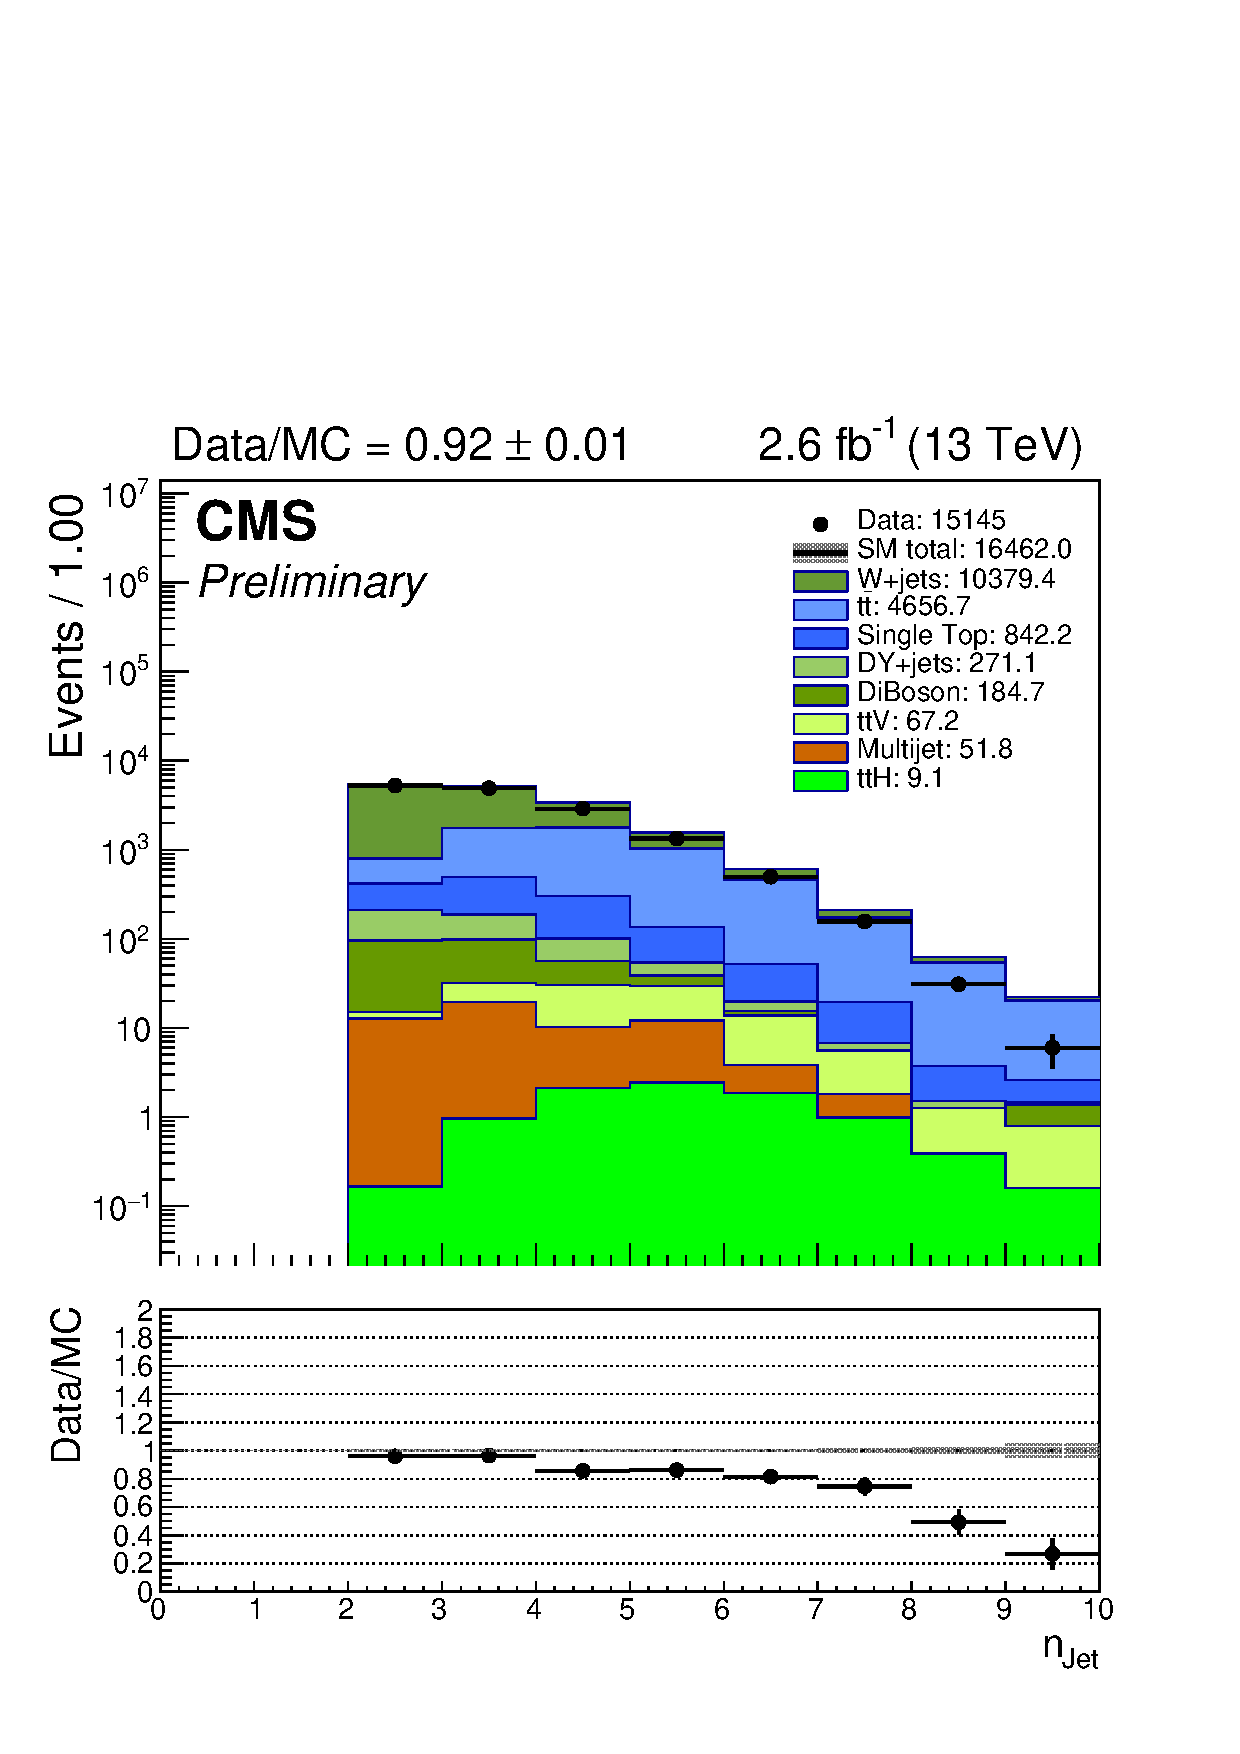
\includegraphics[width=0.5\textwidth]{figures/distributions/Signal/nJet40_sym.pdf}} ~~
        \subfigure {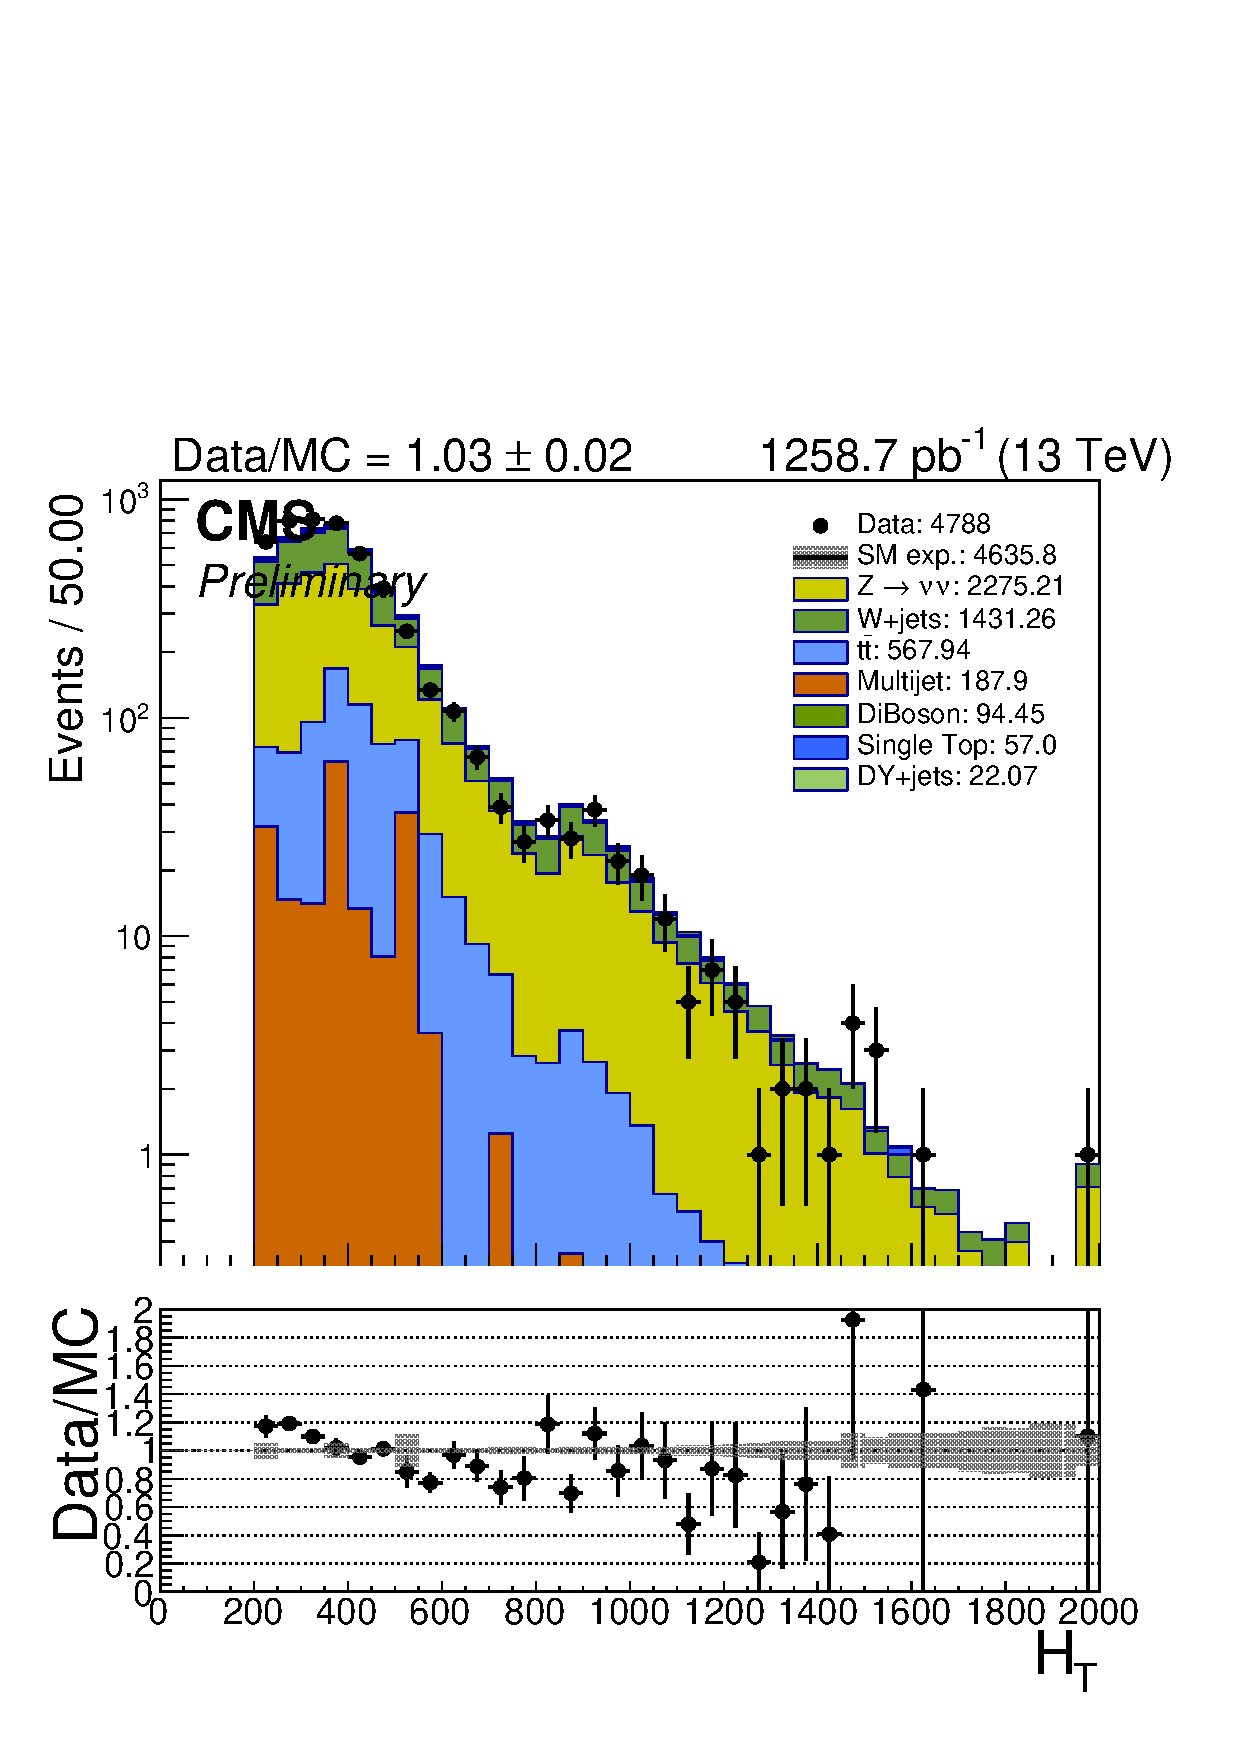
\includegraphics[width=0.5\textwidth]{figures/distributions/Signal/ht40_sym.pdf}} \\
        \subfigure {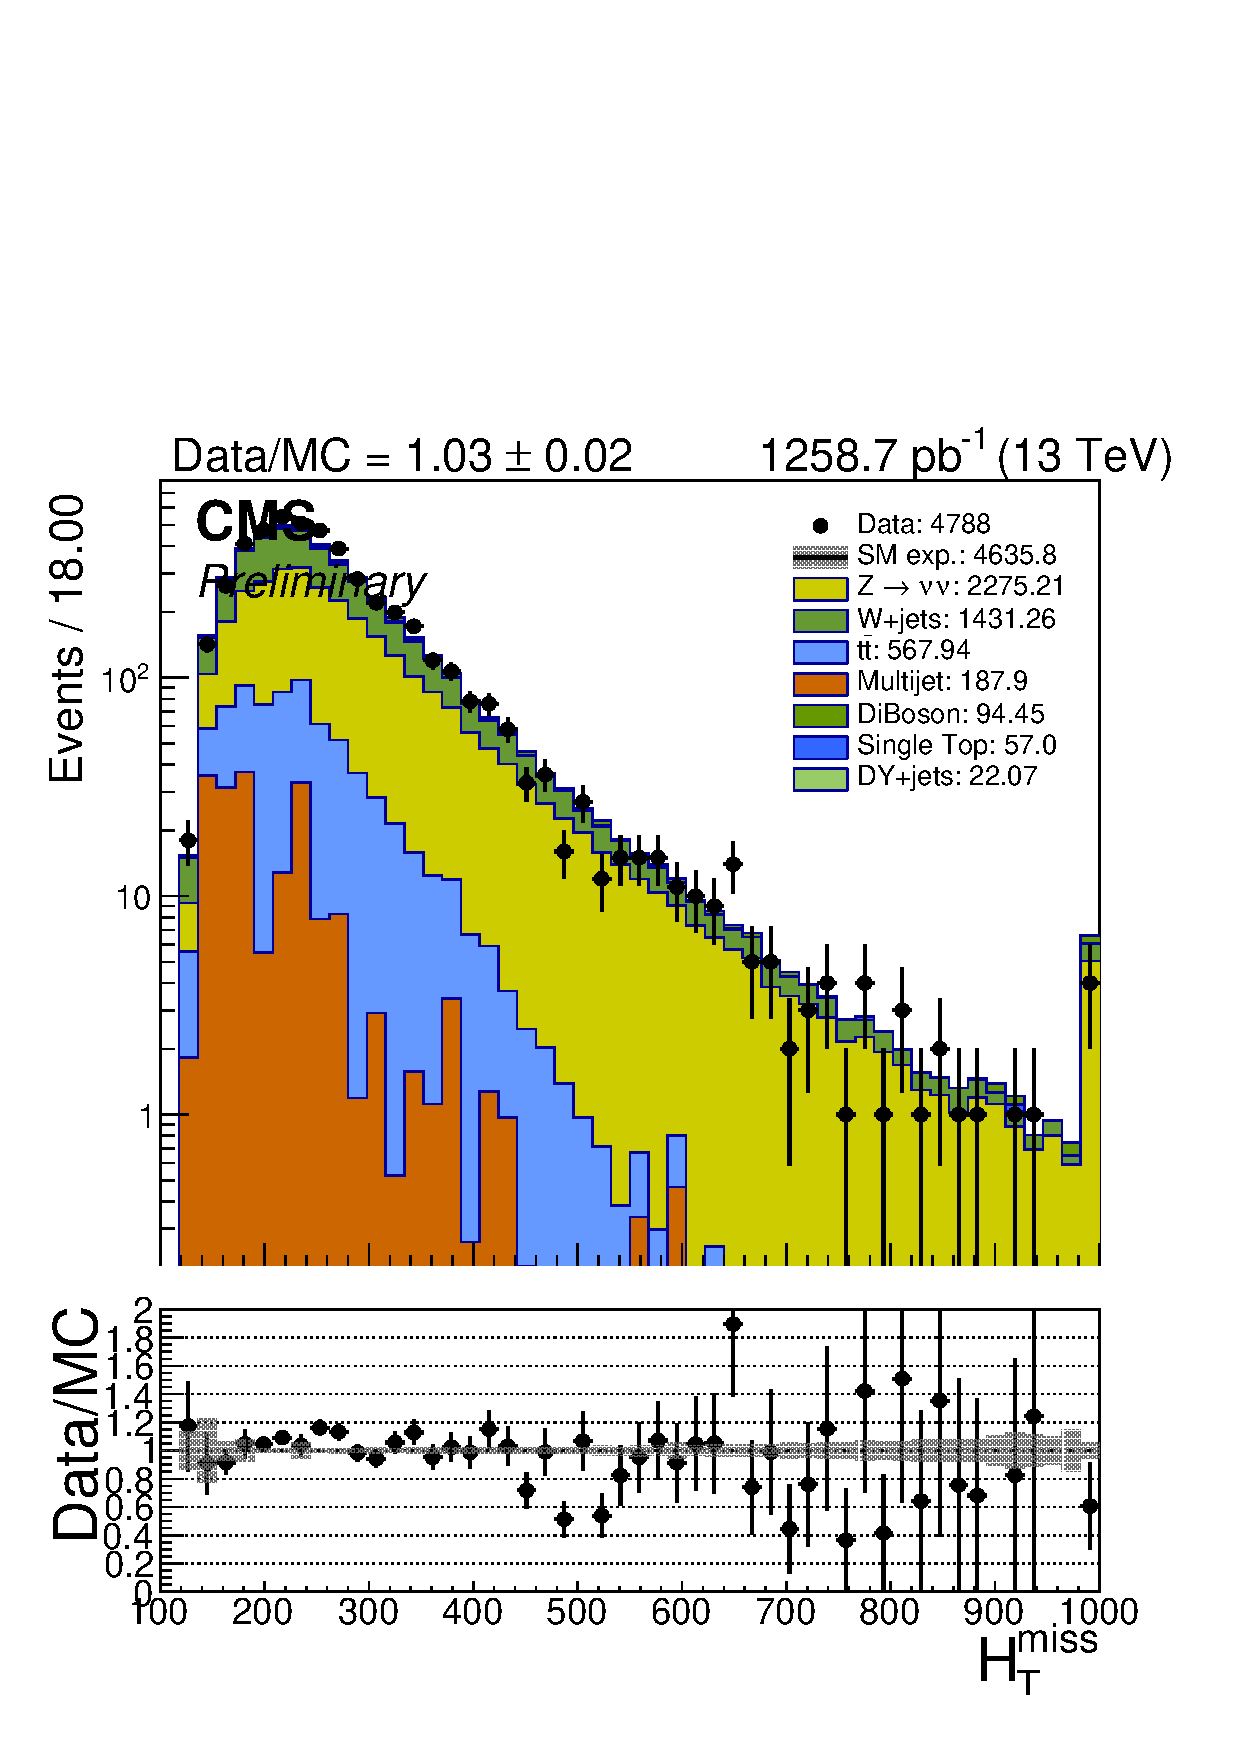
\includegraphics[width=0.5\textwidth]{figures/distributions/Signal/mht40_pt_sym.pdf}} ~~
        \subfigure {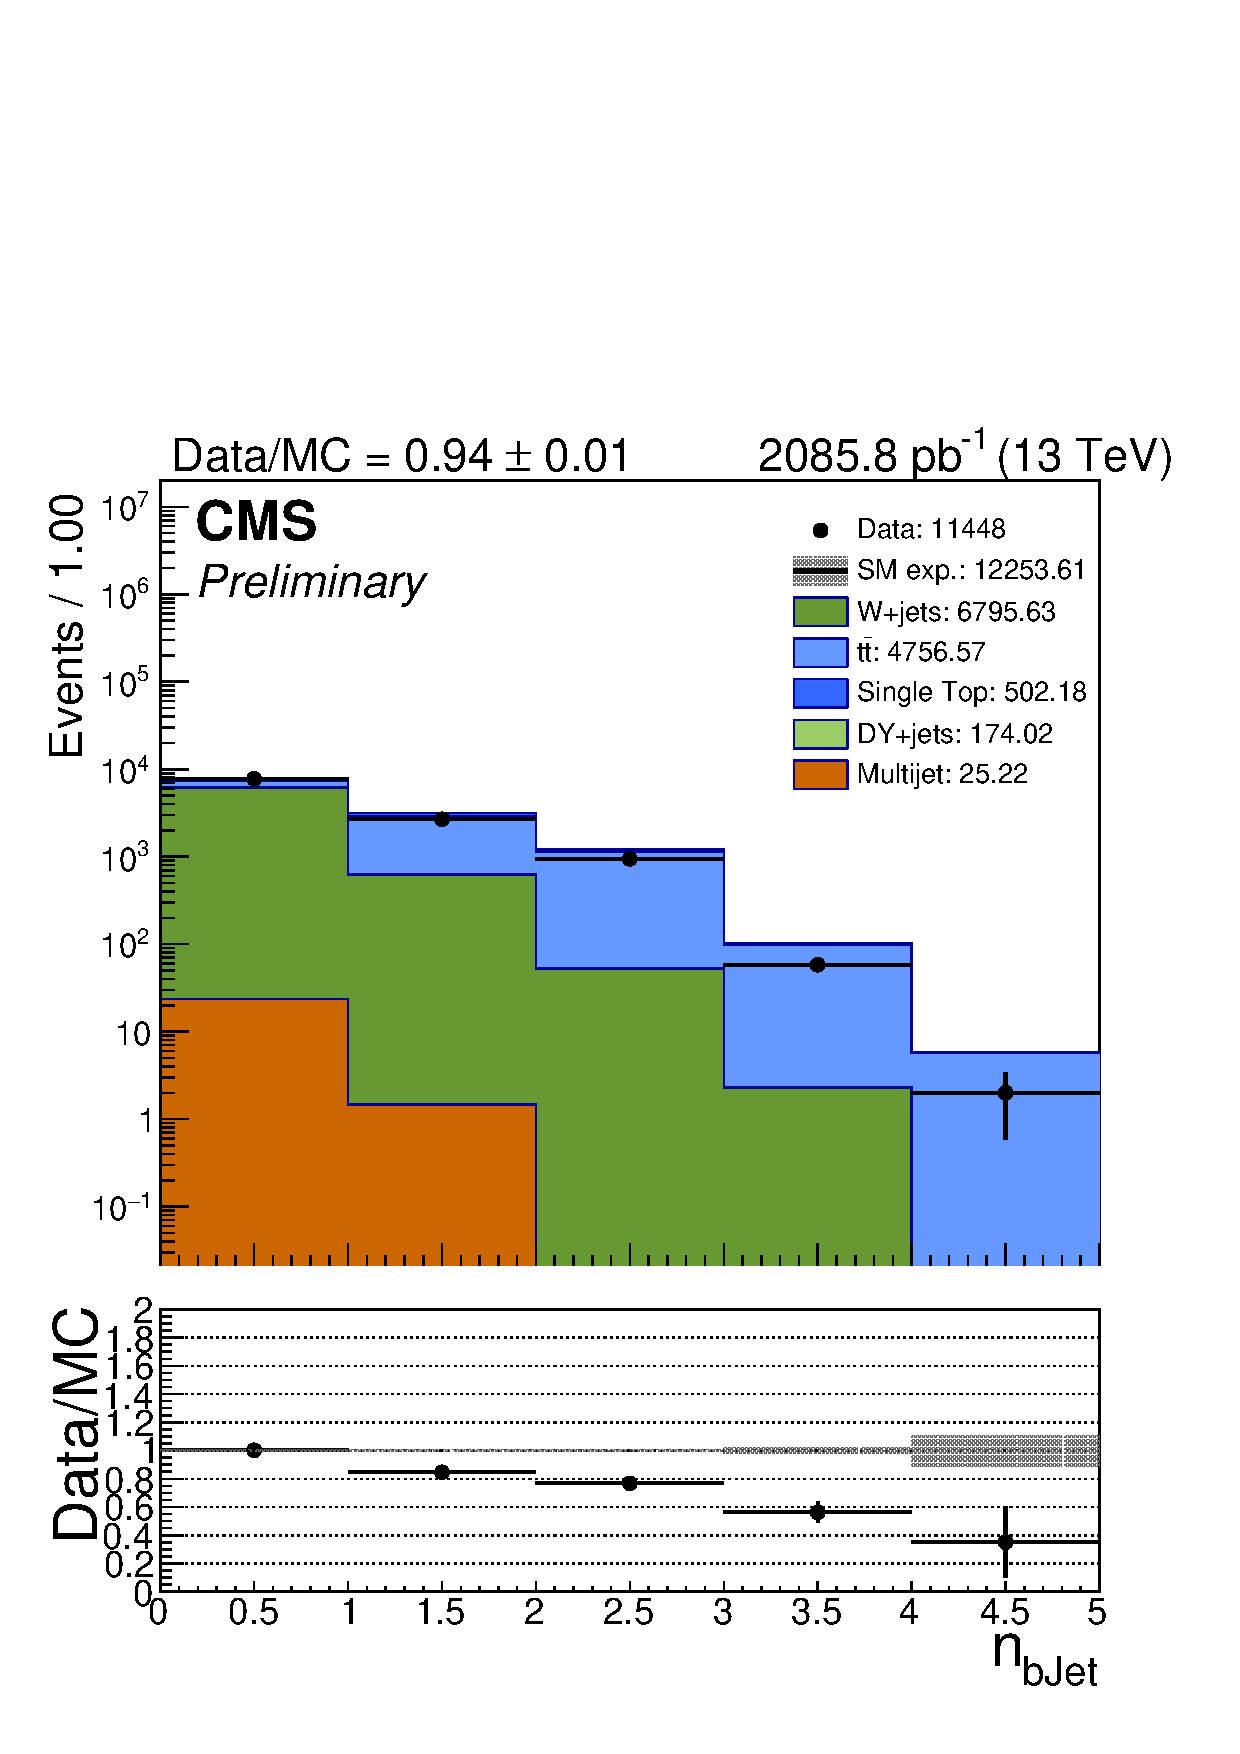
\includegraphics[width=0.5\textwidth]{figures/distributions/Signal/nBJetMedium40_sym.pdf}} \\
        \caption{Key analysis variables for hadronic signal region (symmetric \njet bins)}
        \label{fig:distribution_signal_sym}
    \end{center}
\end{figure}

\clearpage
\begin{figure}
    \begin{center}
        \subfigure {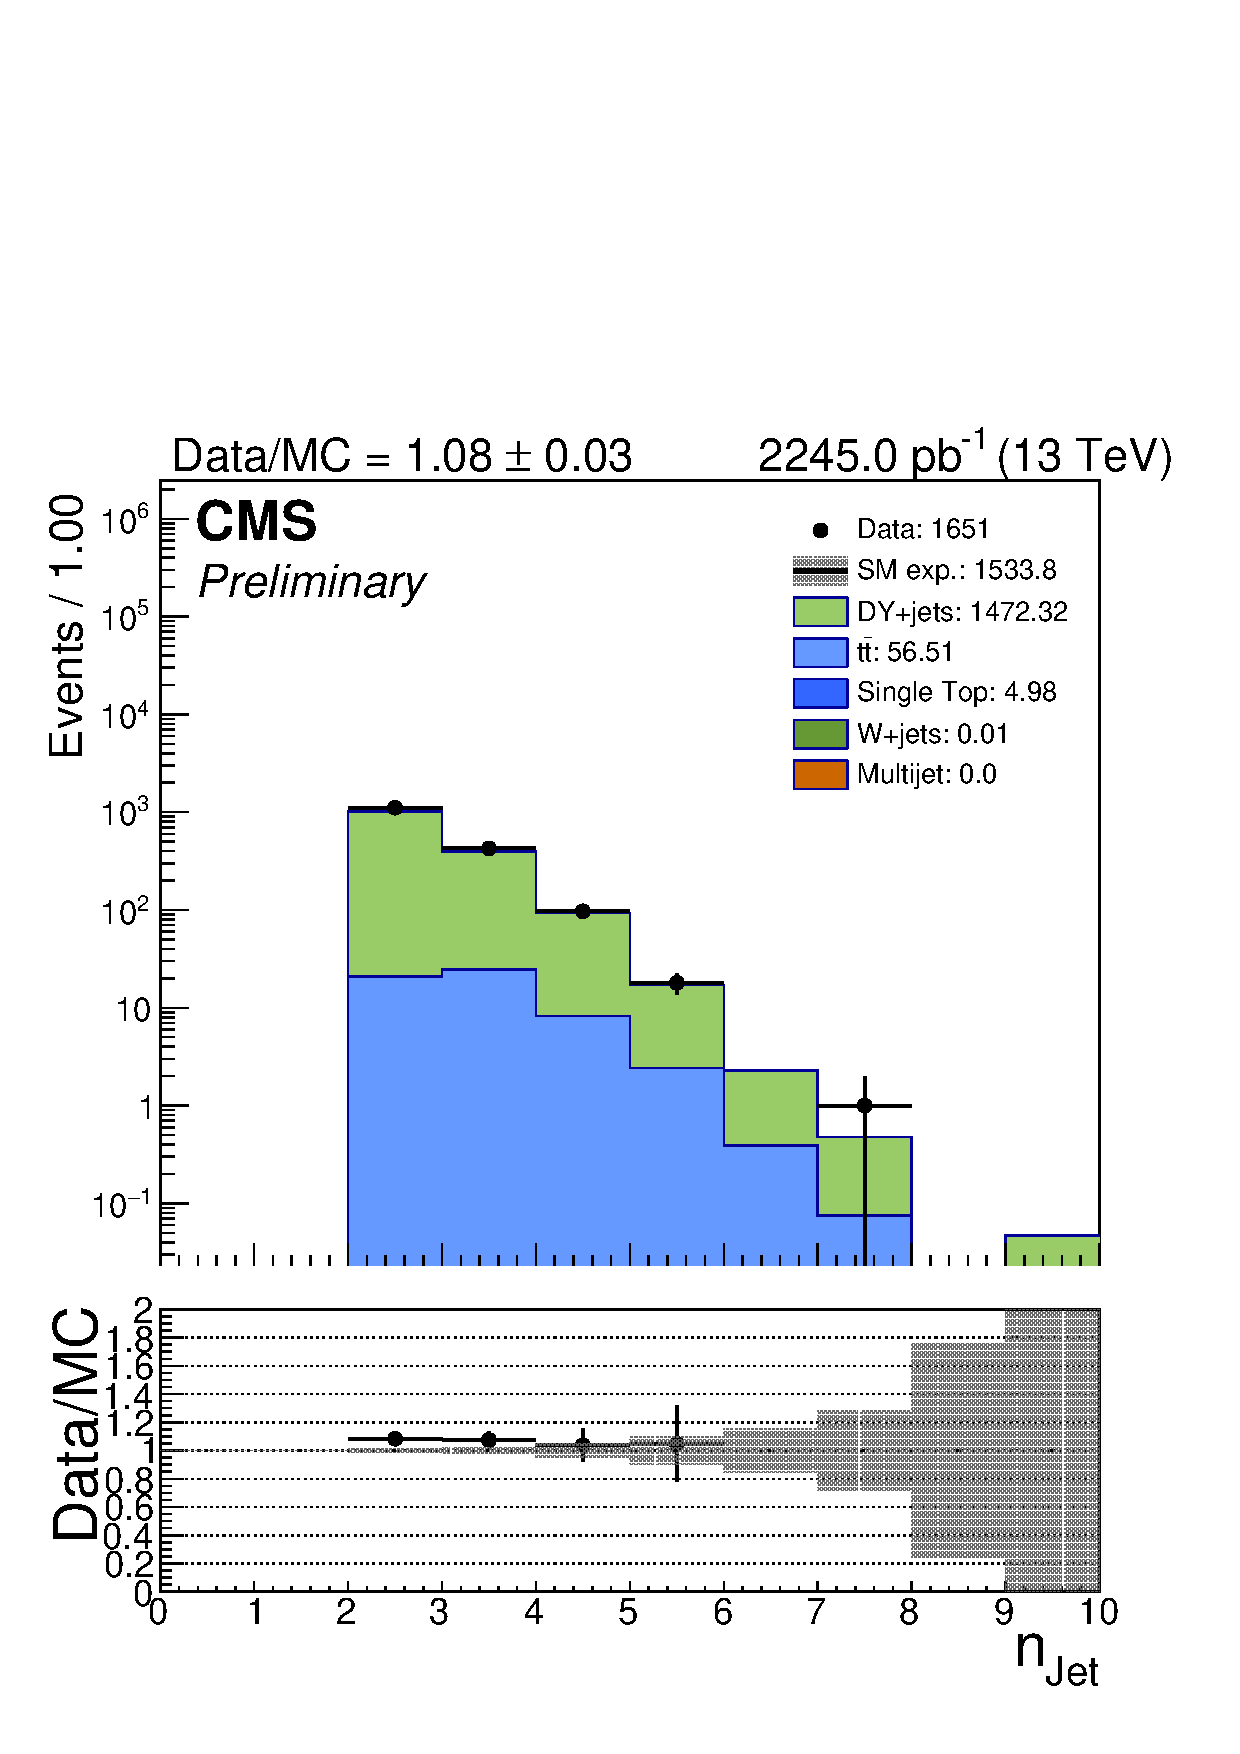
\includegraphics[width=0.5\textwidth]{figures/distributions/Signal/nJet40_asym.pdf}} ~~
        \subfigure {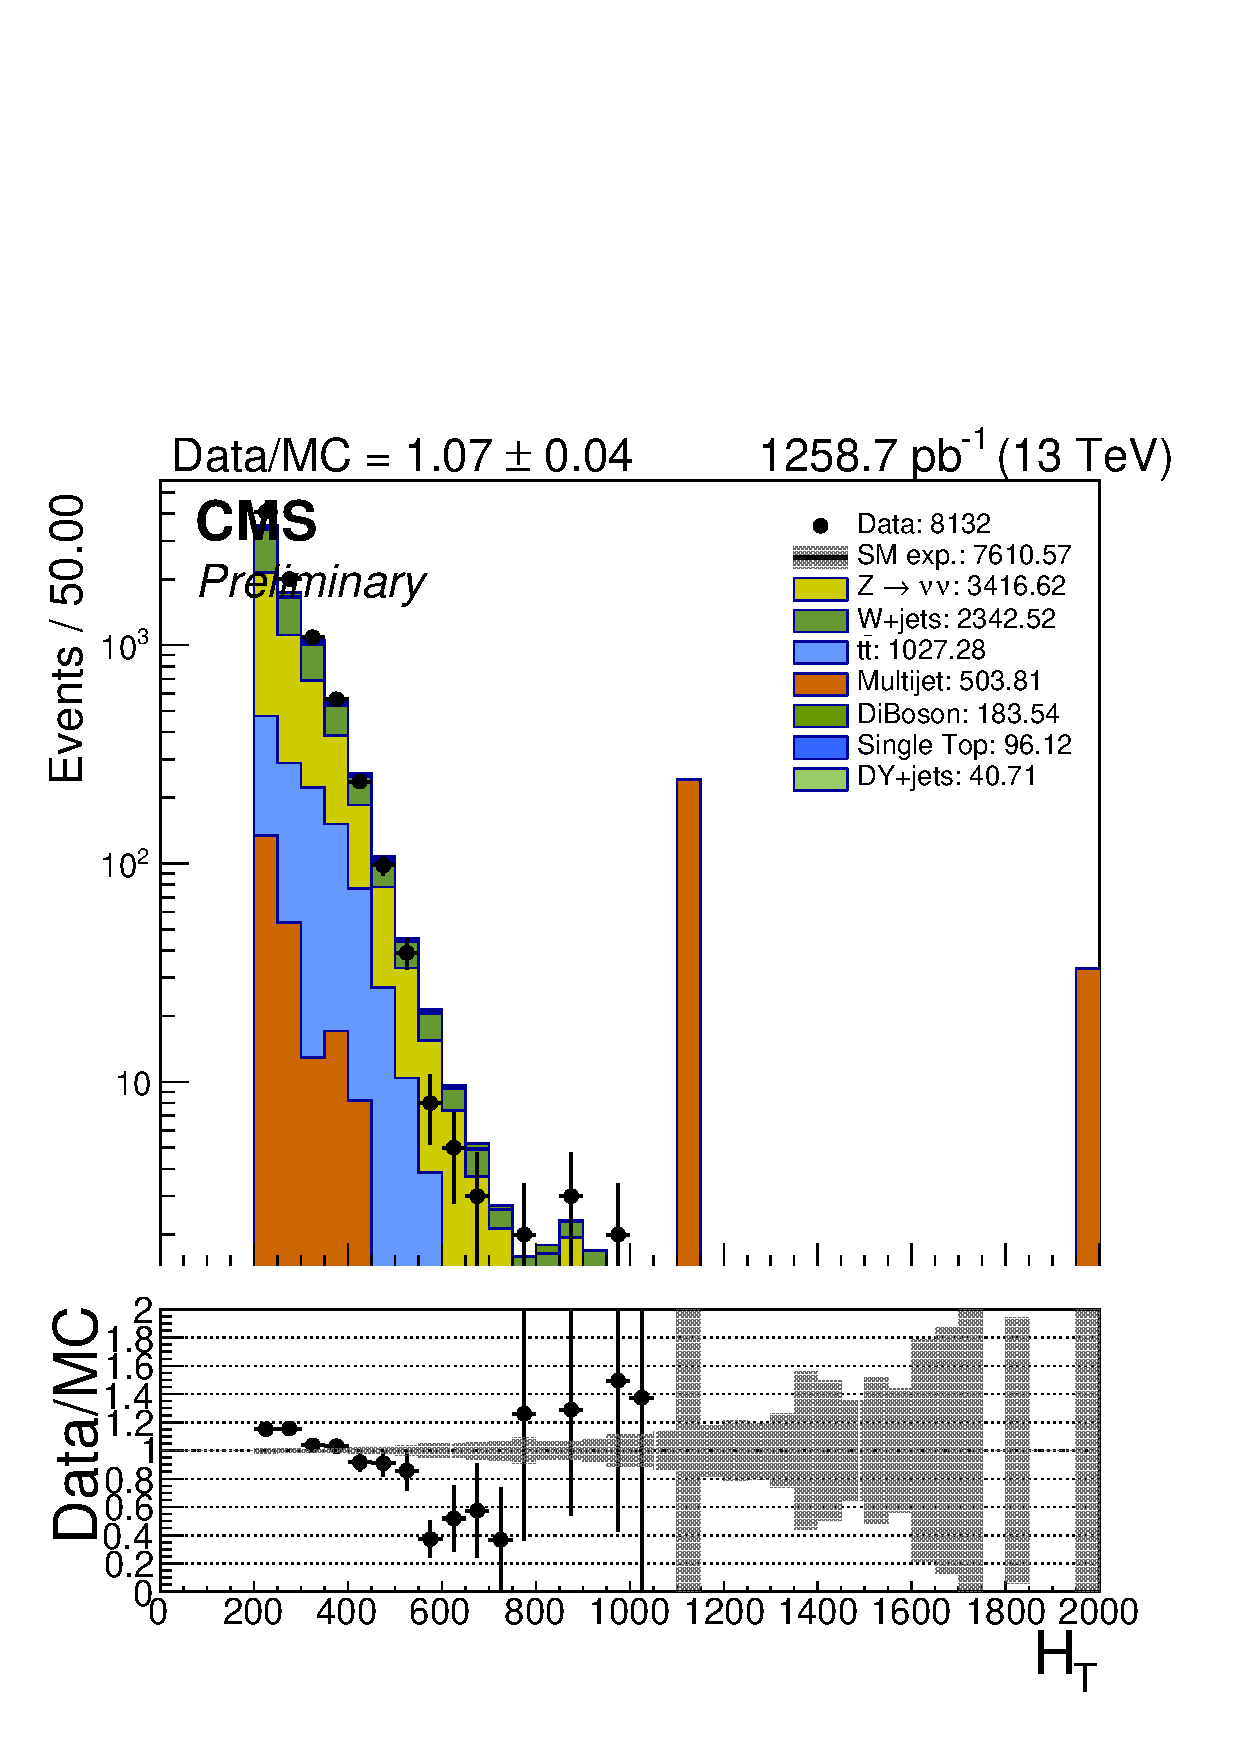
\includegraphics[width=0.5\textwidth]{figures/distributions/Signal/ht40_asym.pdf}} \\
        \subfigure {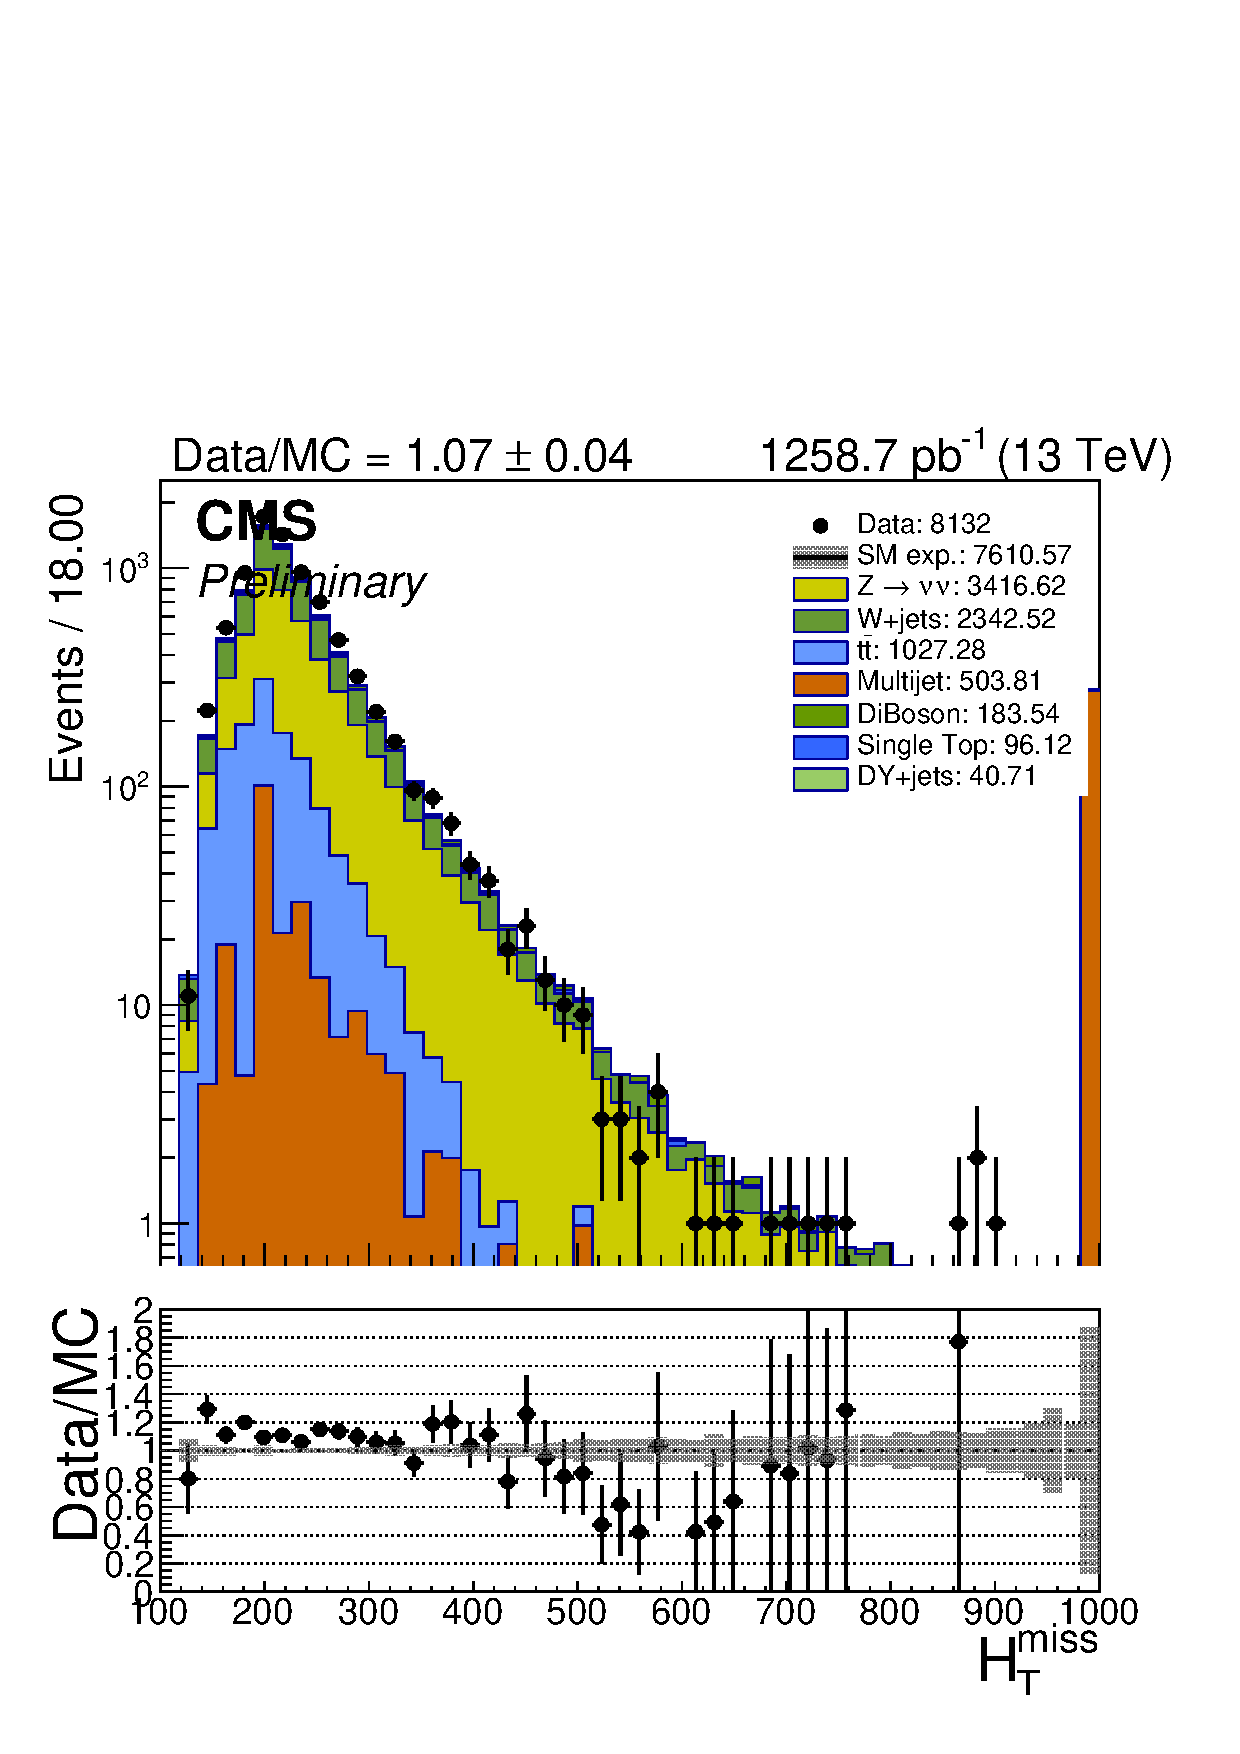
\includegraphics[width=0.5\textwidth]{figures/distributions/Signal/mht40_pt_asym.pdf}} ~~
        \subfigure {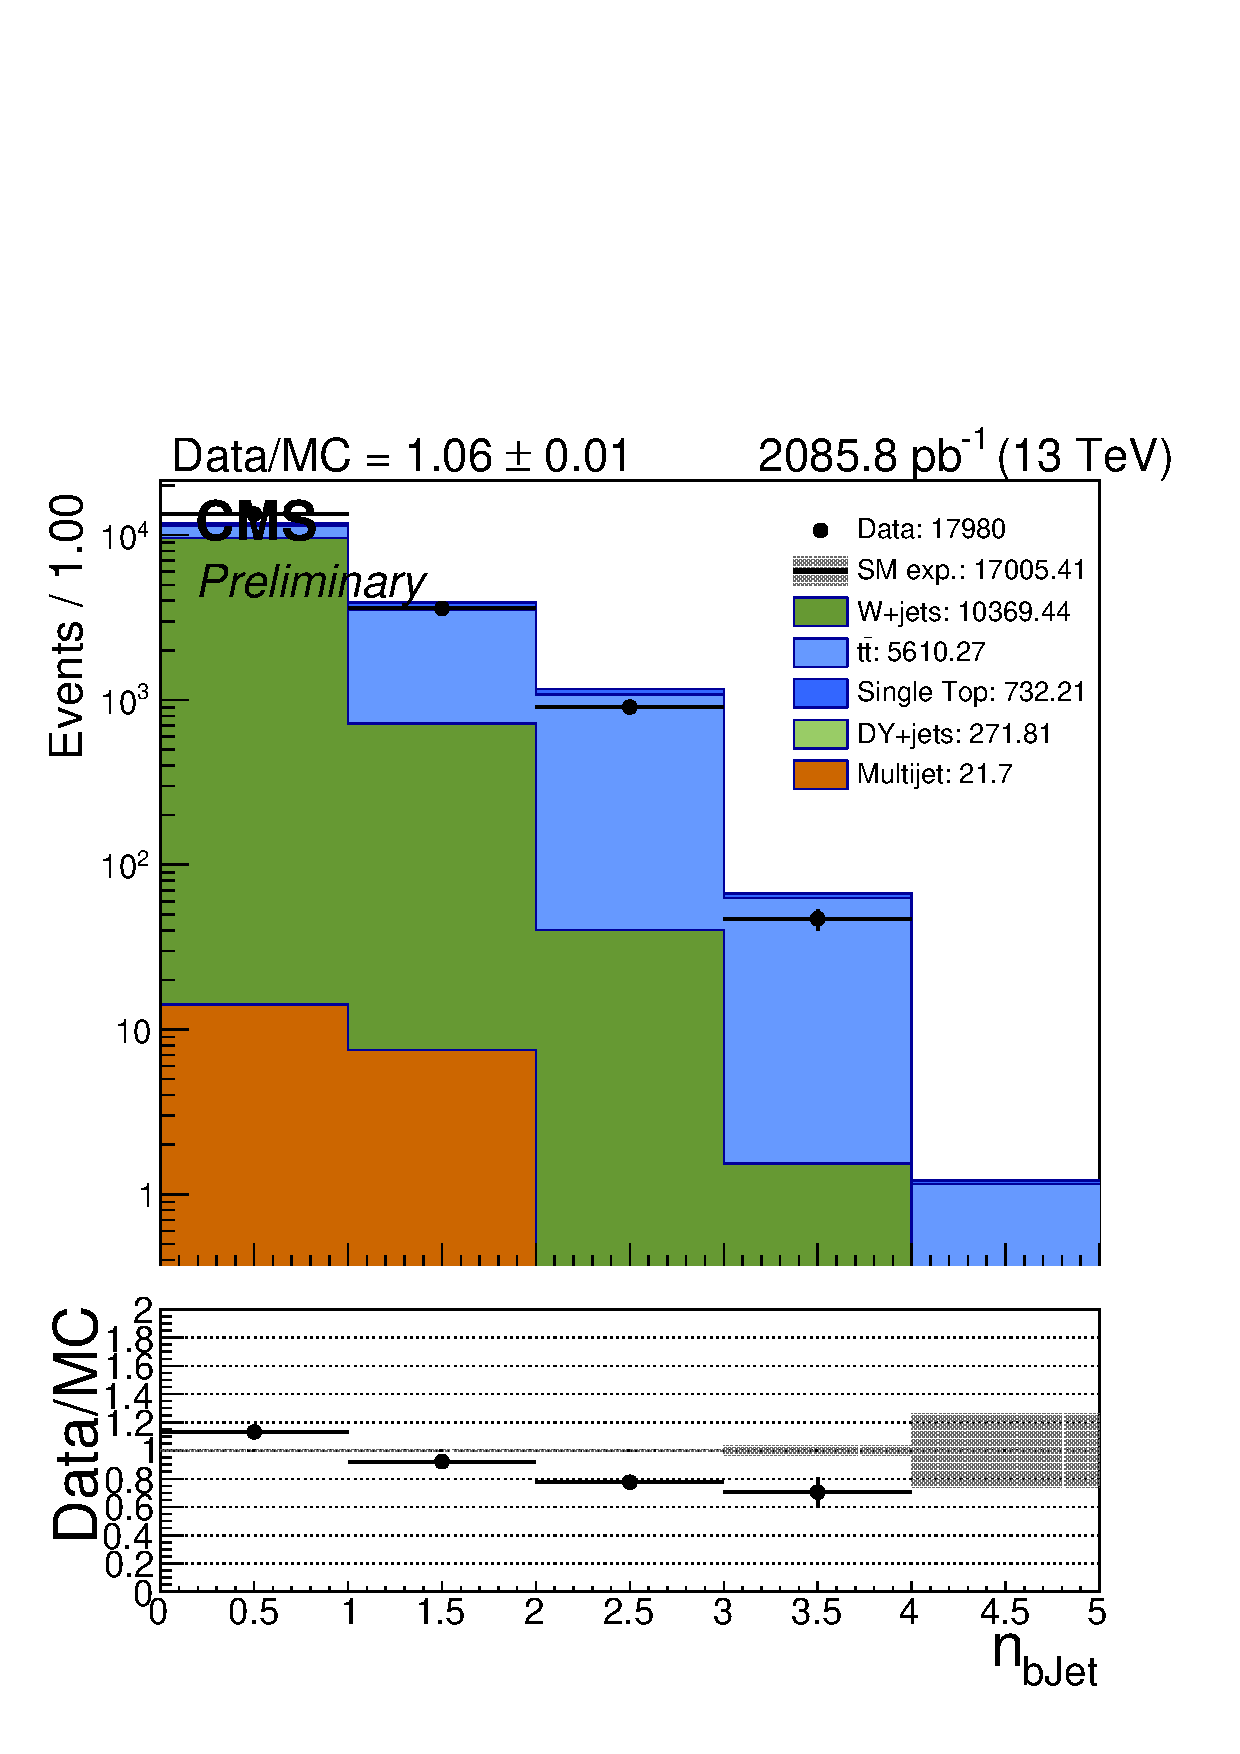
\includegraphics[width=0.5\textwidth]{figures/distributions/Signal/nBJetMedium40_asym.pdf}} \\
        \caption{Key analysis variables for hadronic signal region (asymmetric \njet bins)}
        \label{fig:distribution_signal_asym}
    \end{center}
\end{figure}

\clearpage
\begin{figure}
    \begin{center}
        \subfigure {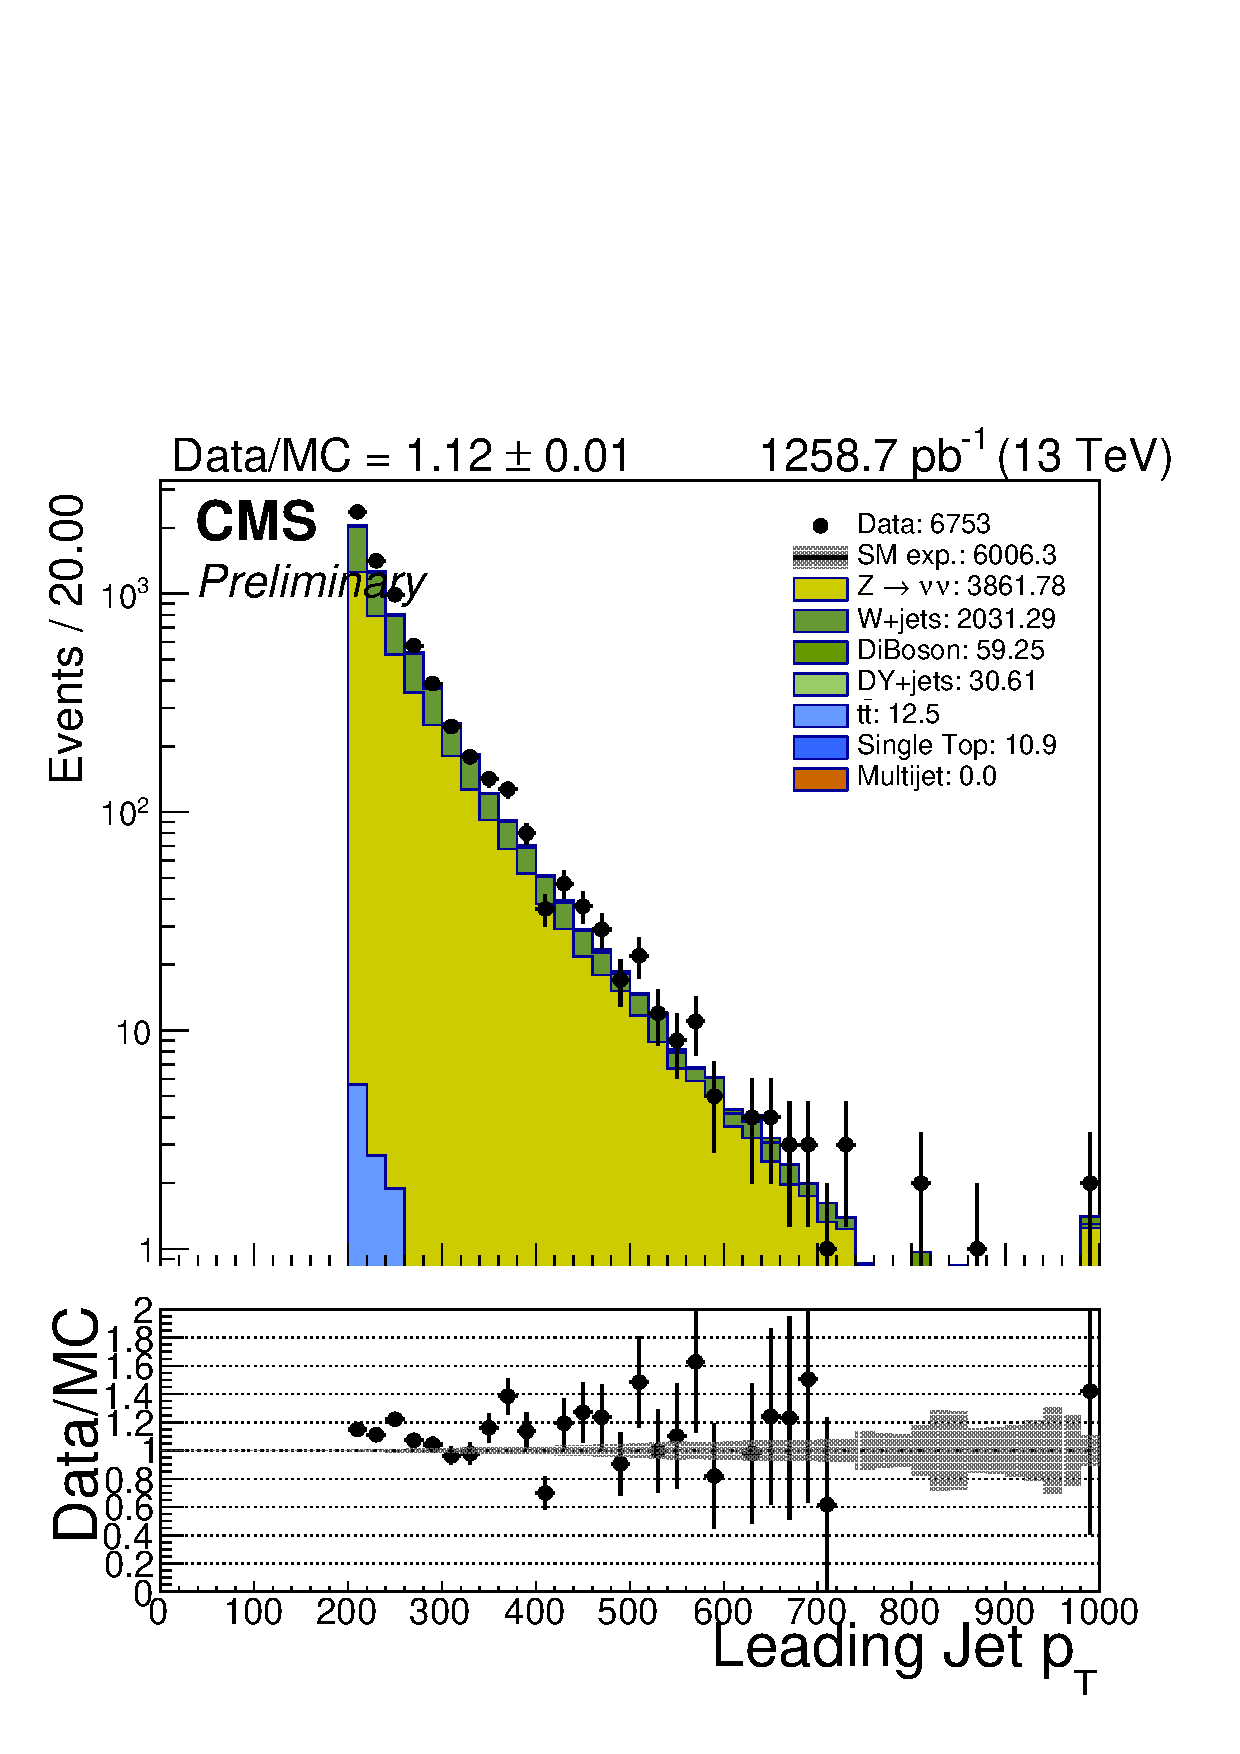
\includegraphics[width=0.5\textwidth]{figures/distributions/Signal/jet_pt[0]_eq1j.pdf}} ~~
        \subfigure {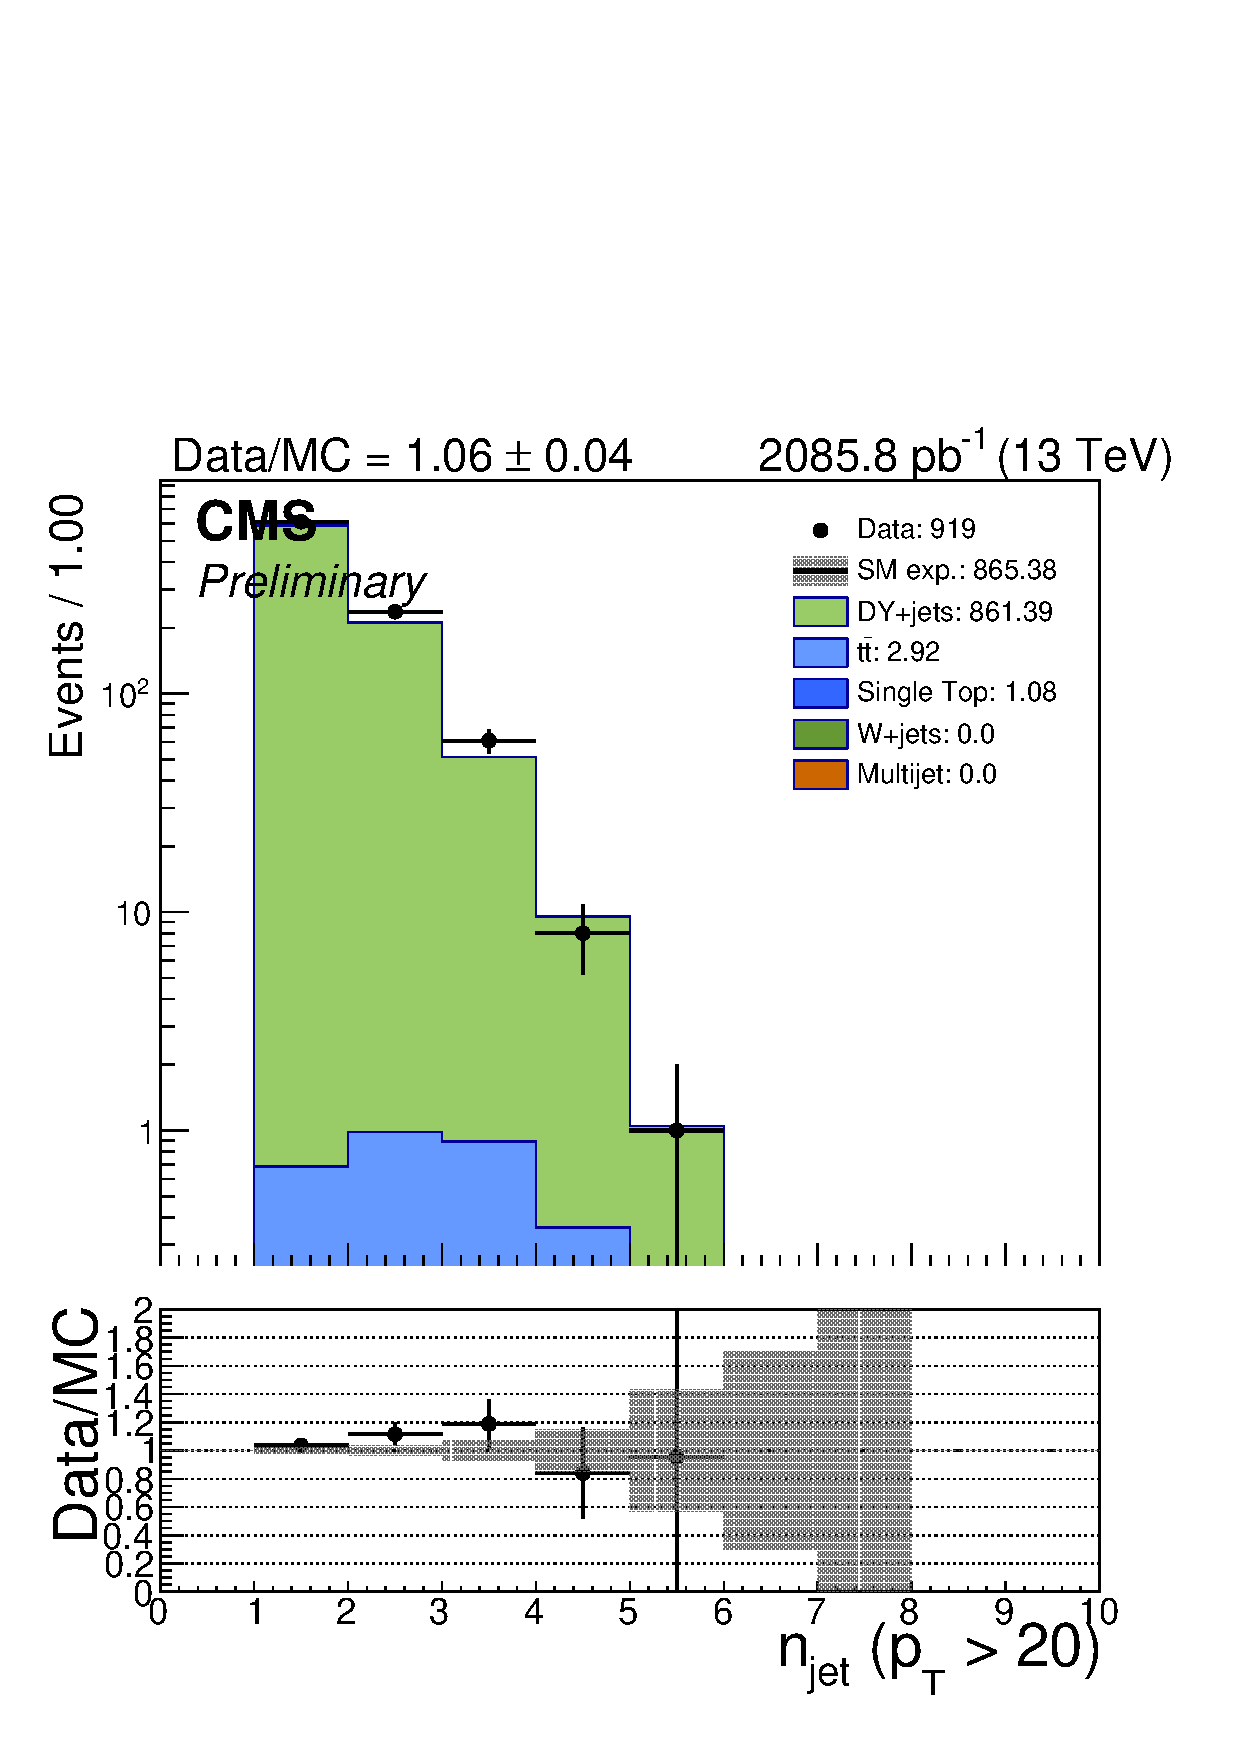
\includegraphics[width=0.5\textwidth]{figures/distributions/Signal/njetInc_eq1j.pdf}} \\
        \subfigure {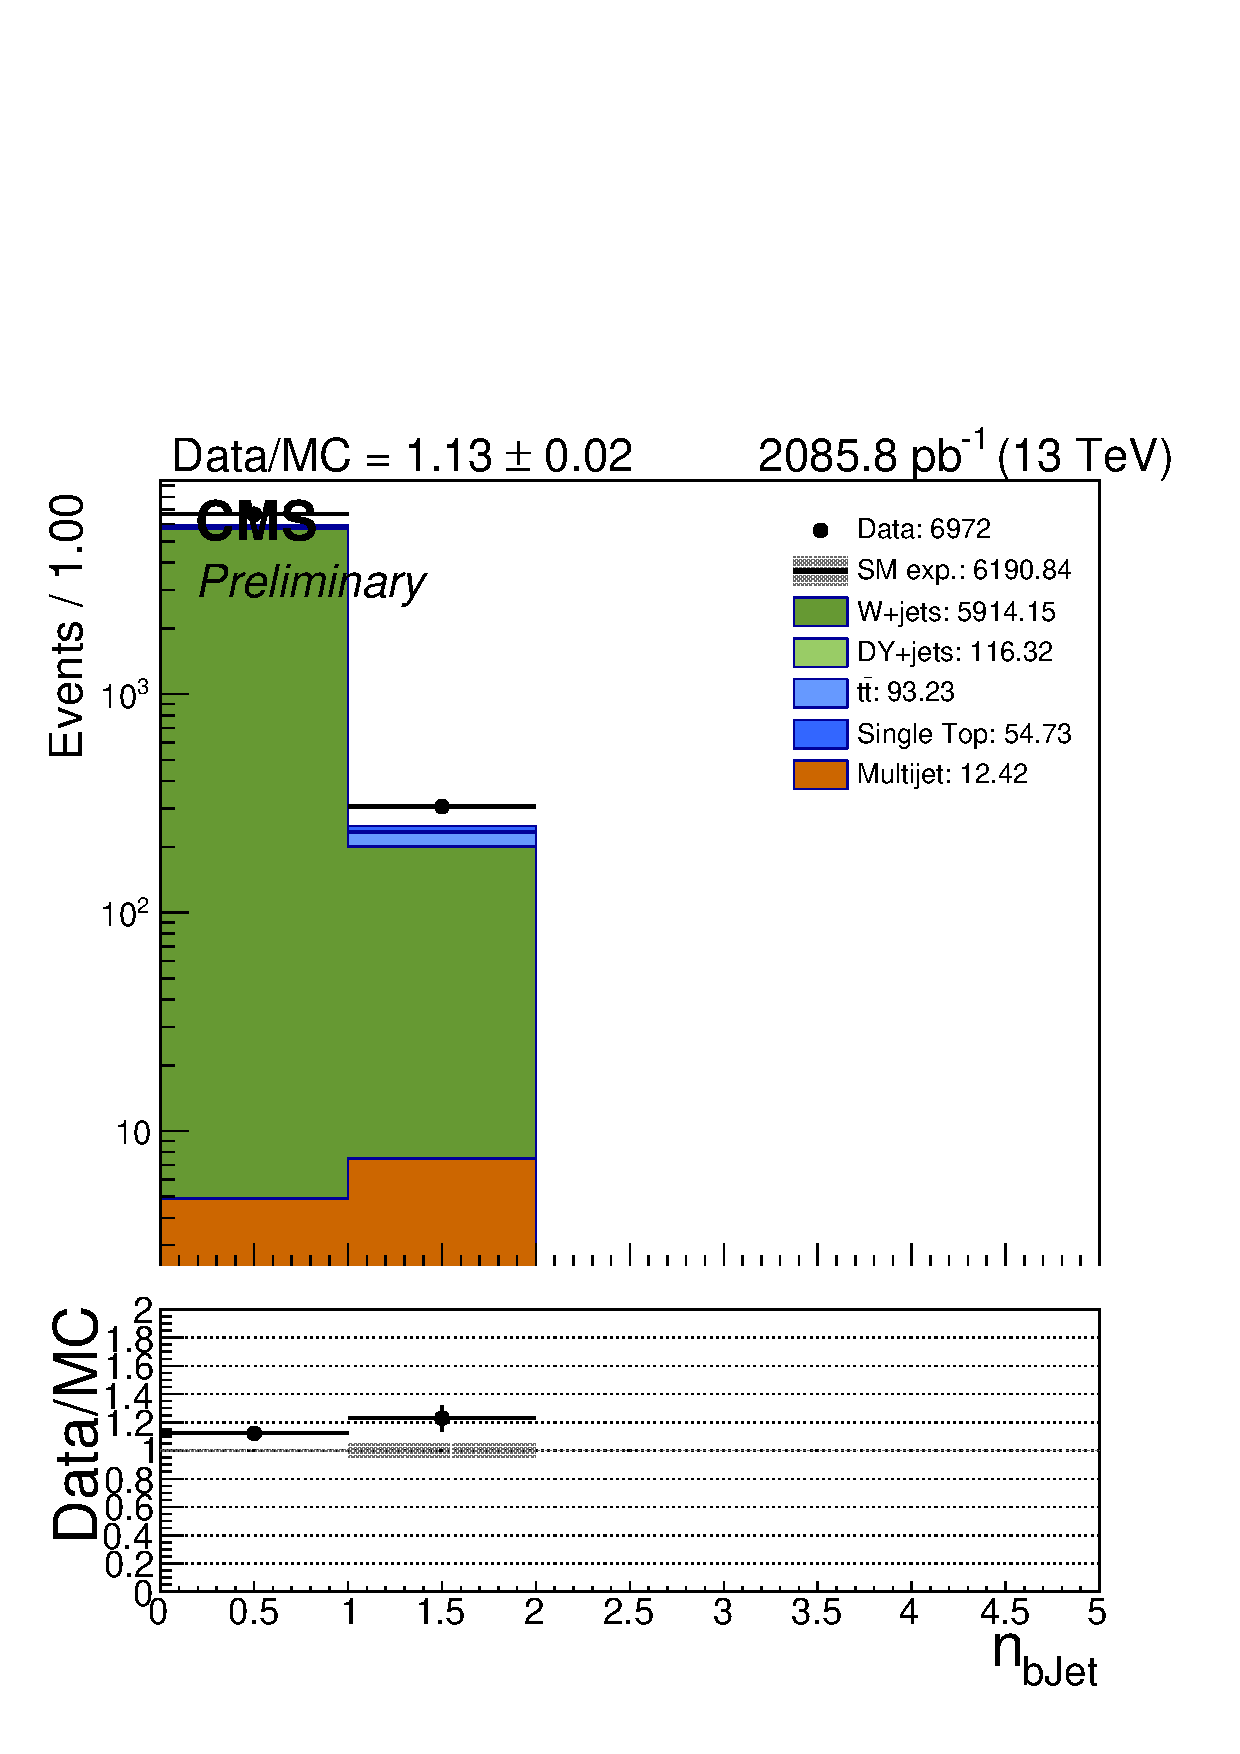
\includegraphics[width=0.5\textwidth]{figures/distributions/Signal/nBJetMedium40_eq1j.pdf}} ~~
        \subfigure {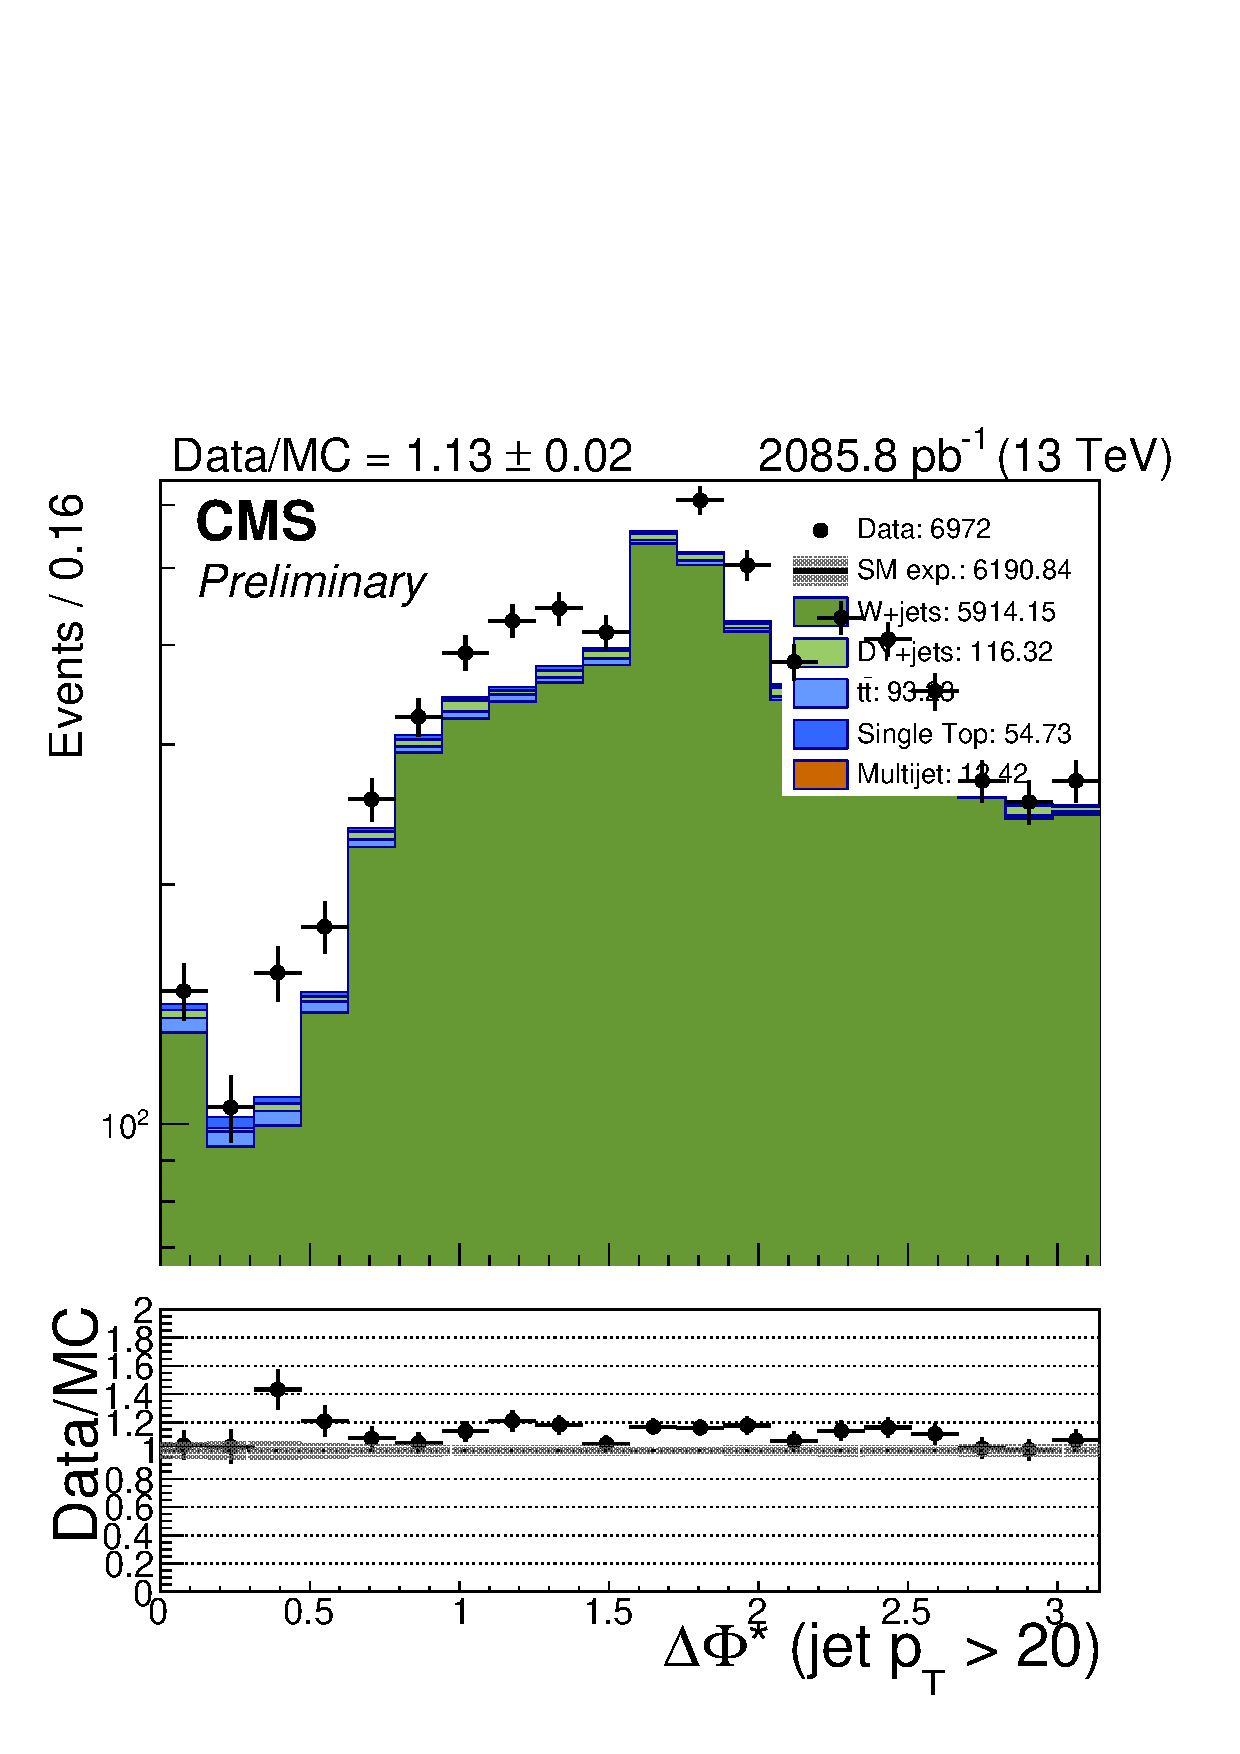
\includegraphics[width=0.5\textwidth]{figures/distributions/Signal/biasedDPhiInc_eq1j.pdf}} \\
        \caption{Key analysis variables for hadronic signal region (monojet bins)}
        \label{fig:distribution_signal_mono}
    \end{center}
\end{figure}




% Overrides original definition
\def\rmhtmet{\mbox{$\mathcal{R}$}\xspace}

%%____________________________________________________________________________||
\section{Background estimation for QCD multijet events \label{sec:qcd}}
\subsection{QCD control with the \bdphi variable}

One of the major challenges for searches of new physics in the jets +
\met final state is the control of background events from QCD multijet
production. The difficulties in the determination of precise estimates
for this background stem from the large cross sections expected in the
high-energy, high-luminosity hadron collider environment at the LHC,
which are further compounded by the lack of precise theoretical
predictions for the cross sections and kinematic properties of
multijet events. Hence, without special consideration and treatment,
significant uncertainties on large background expectations can
overwhelm any potential sensitivity to new physics signatures.

With regards to QCD multijet production, the approach of this search
is to favour the suppression of the multijet background to a
negligible level over the goal of high efficiency for any given signal
model. A conservative uncertainty on a negligible contribution is
preferred over a procedure that attempts to accurately estimate a
non-negligible contribution from multijet events. The level of
contamination should be sufficiently small (\ie sub-percent level)
such that the associated uncertainty, even if large, will be
sub-dominant with respect to the uncertainties on the remaining SM
backgrounds with genuine \met such as \wj, \znunu, and \ttbar,
henceforth labelled as non-multijet processes.

Any contamination from QCD multijet events is controlled primarily
through the \alphat and \bdphi variables. The \alphat variable is able
to distinguish with high efficiency the sources of ``fake'' \met, such
as jet energy mismeasurement, from those with ``genuine'' \met, such
as neutrinos. The \bdphi variable is also very efficient at
identifying jets that suffer under-measurements, as well as
over-measurements, in (otherwise balanced) multijet events. The
variable is also particularly suited to identifying multijet events
that exhibit significant \met due to the production of neutrinos
(collinear with a jet axis) in semileptonic heavy-flavour decays. Both
variables are individually capable of reducing the yields from
multijet events by several orders of magnitude, and combined provide
an extremely robust method to reject multijet events.

In Fig.~\ref{fig:bDPhi_nominal} a comparison of the abilities of the \bdphi variable to 
control the QCD multijet background with 
a similar jet-\mht angular variable \dphimhtj, the minimum azimuthal separation between the \mht-vector and the leading four
jets, is presented. The \bdphi variable exhibits a distribution that
is more sharply peaked for the QCD multijet background 
at low values and faster falling than \dphimhtj,  \dphimhtj for QCD conversely has a broader 
distribution with a larger leakage for a comparable azimuthal
selection. This demonstrates the ability of \bdphi to provide a better
control of the QCD background while retaining acceptance of events with genuine \mht,
in this case represented by the V+jets, \ttbar and other residual SM
backgrounds with genuine \met. 

This is
further demonstrated in Fig.~\ref{fig:bDPhi_roc}, where the efficiency
of retaining processes with genuine \mht is plotted against the
background efficiency for a series of \bdphi, \dphimhtj and
\dphimhtjall cuts, where \dphimhtjall considers all jets rather than
just the leading four. The
points with a cut of $0.5$ are highlighted as stars on the plot. The
general analysis strategy involves reducing the QCD multijet
background to a negligible level while maximising signal acceptance. These plots demonstrate that this is
most achievable with a cut on \bdphi. For the same threshold
requirement of $0.5$ on each variable, the \bdphi variable provides an
efficiency for multijet events that is approximately three orders of
magnitude lower than for \dphimhtj at the cost of approximately a factor $3$
reduction in signal efficiency. The threshold on \bdphi required to give
an approximately equivalent suppression of QCD achieved with the
\dphimhtj
variable is larger than 1.5, at the cost of a loss of a factor $5$ in
signal acceptance w.r.t. \bdphi. This also holds true in the extreme
case of a high jet multiplicity signal model. Additionally, despite
performing similarly to \bdphi for separating the non-multijet from
multijet backgrounds, the \dphimhtjall variable performs worse for a
high jet multiplicity signal model than \bdphi.

Additionally the \bdphi variable displays robustness in the 
presence of severe event mismeasurement. A mismeasurement is simulated by artificially lowering 
the \pt of the jet that minimises the azimuthal separation variable to 41 \GeV and the event 
variables recomputed. Due to the removal of the probe jet from the computation of \bdphi, the 
distribution of angular separation Fig.~\ref{fig:shifted_bDPhi_dist} is 
remains unchanged under severe mismeasurement. The \dphimhtj variable is
 sensitive to such mismeasurement as both \mht and the rank of the 
leading four jets are affected, resulting in a broader distribution with
increased leakage Fig.~\ref{fig:shifted_DPhiMht_dist}.

\begin{figure}[!h]
 \centering
 \subfigure[\bdphi distribution.\label{fig:bDPhi_dist}]{
 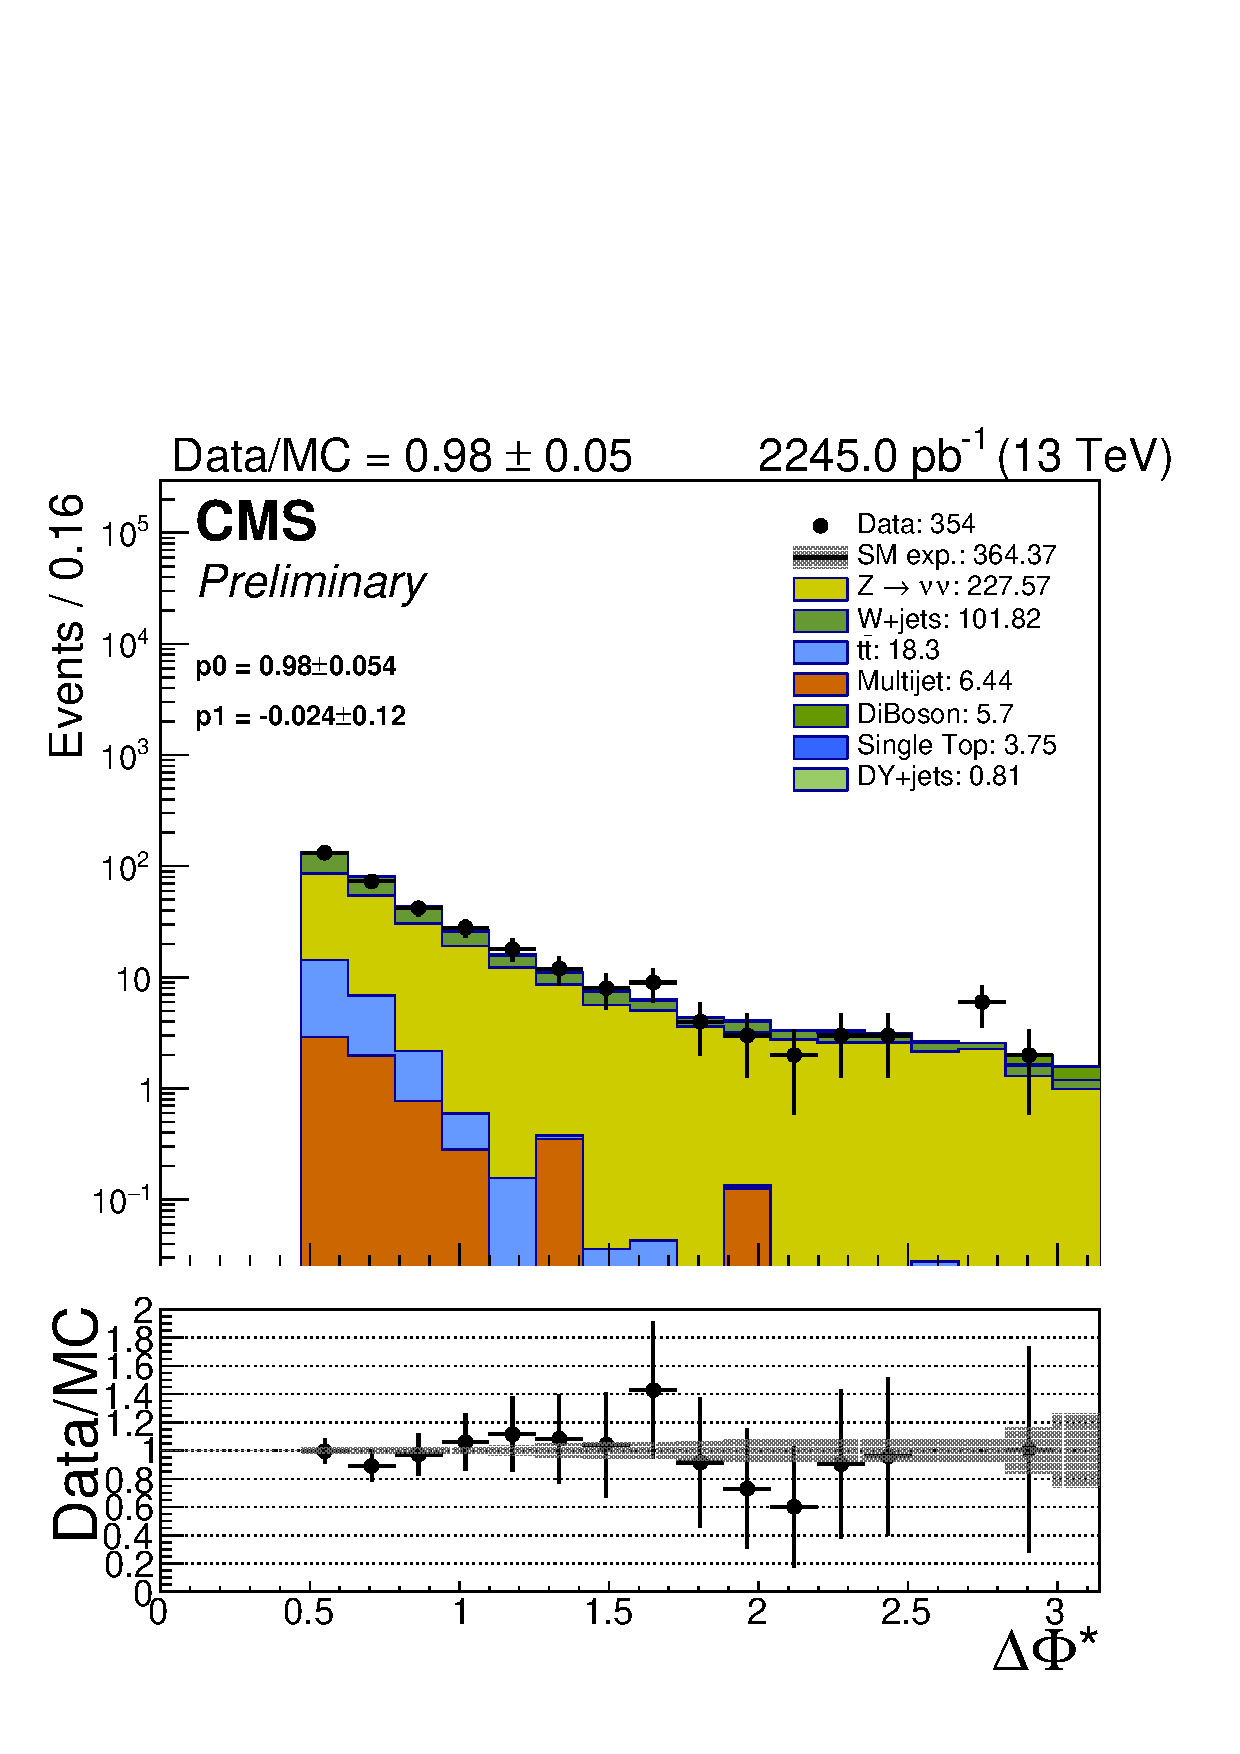
\includegraphics[width=0.5\textwidth]{figures/qcd/biasedDPhi_all_800}
 }
 \subfigure[\dphimhtj distribution.\label{fig:DPhiMht_dist}]{
 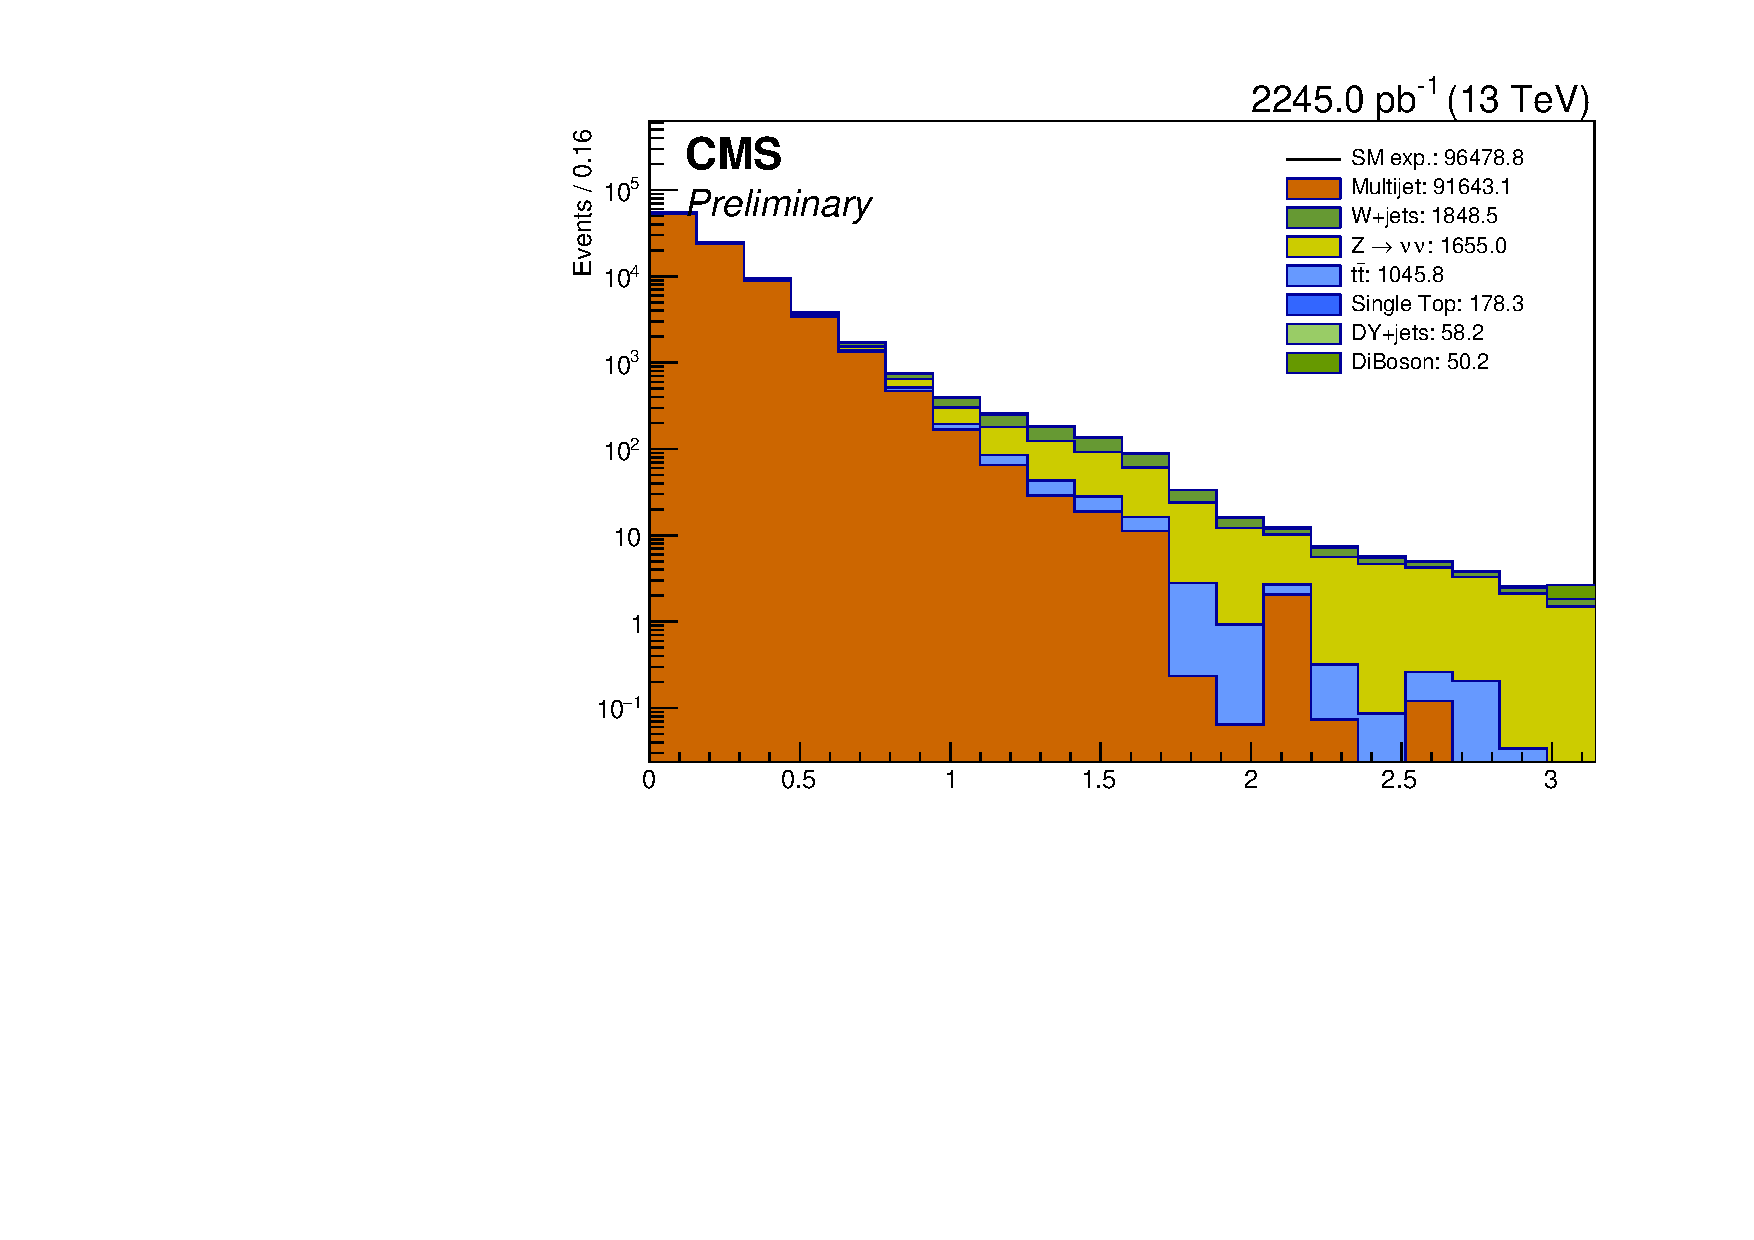
\includegraphics[width=0.5\textwidth]{figures/qcd/minDeltaPhiMht_all_800}
 } \\
 \caption{\bdphi and \dphimhtj distributions of MC simulation of the
 dominant analysis backgrounds
 after analysis selections for \scalht $> 800$ \GeV. }
 \label{fig:bDPhi_nominal}
\end{figure}

\begin{figure}[!h]
 \centering
 \subfigure[Acceptance of SM backgrounds with genuine \met vs QCD
 acceptance]{
 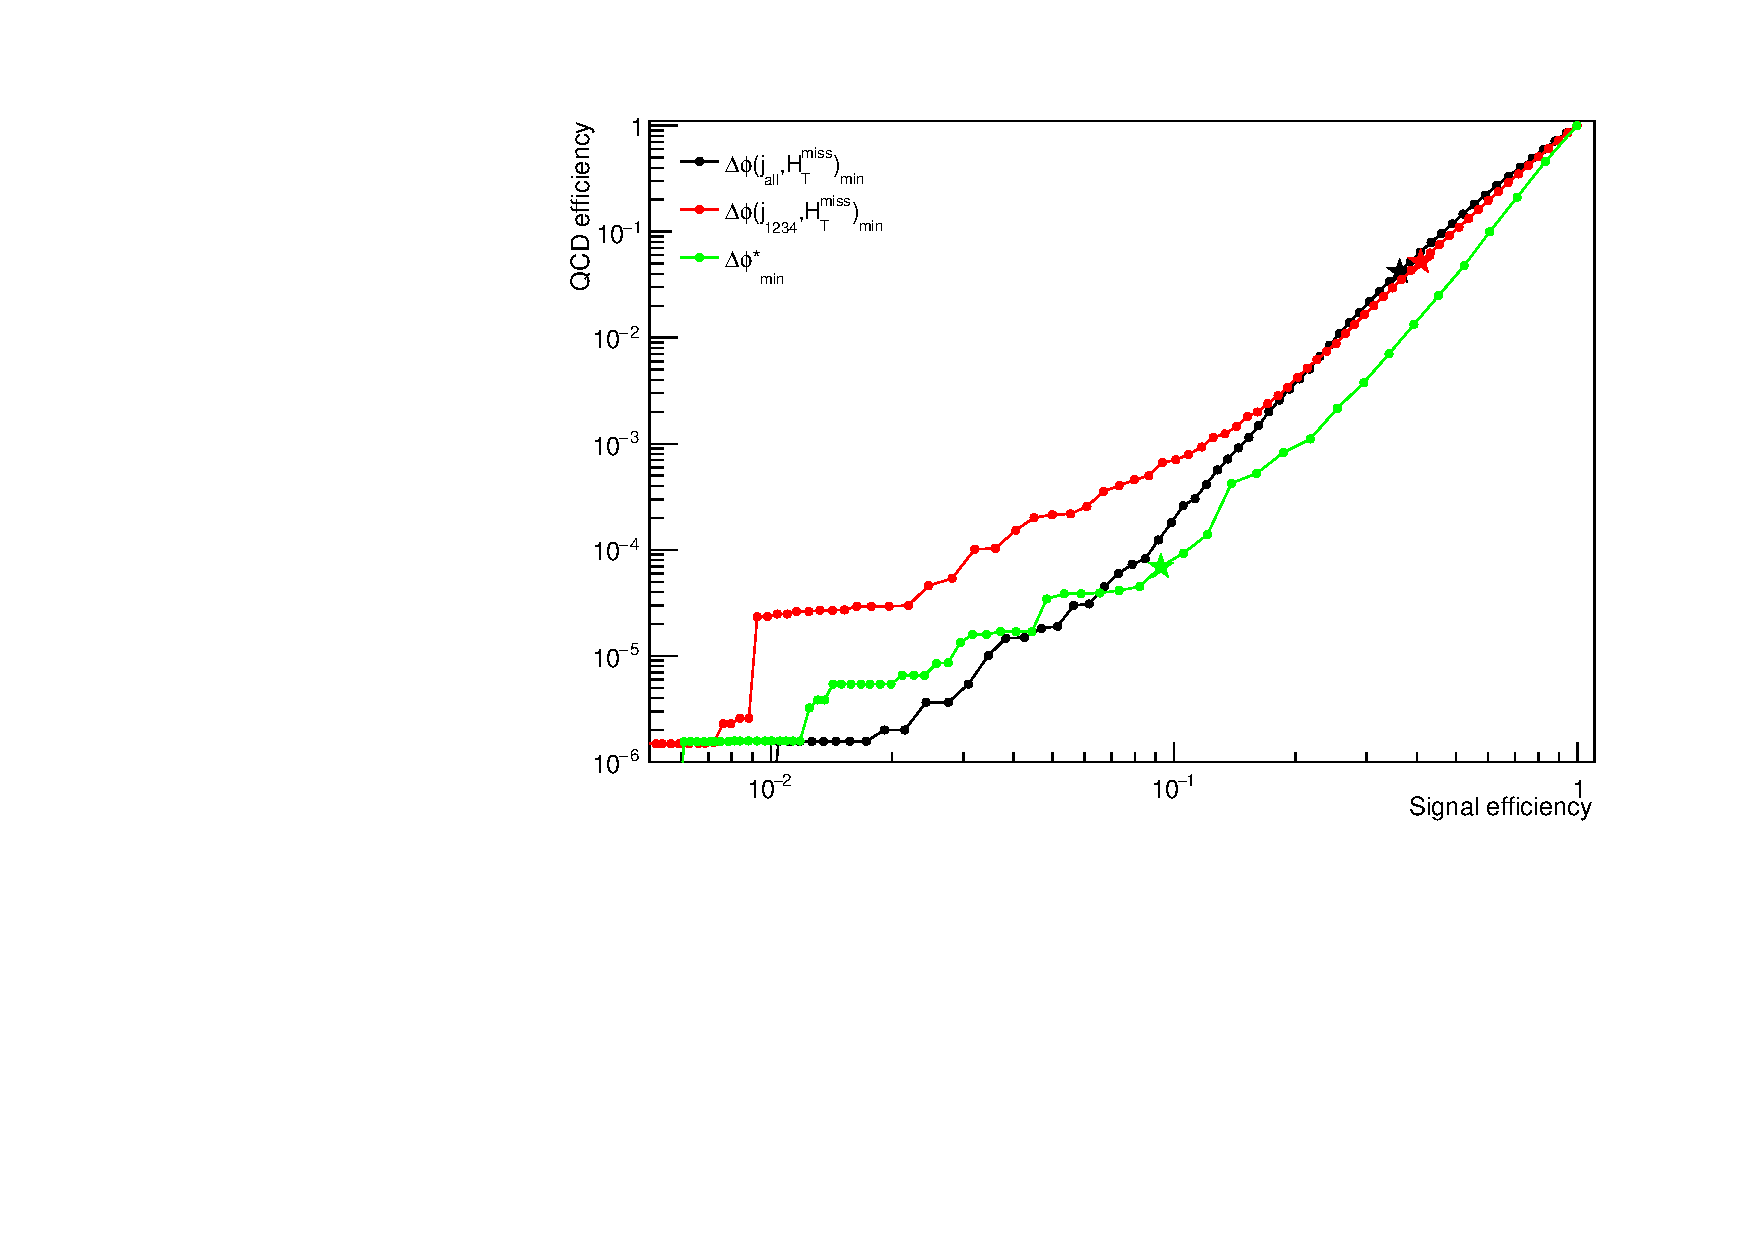
\includegraphics[width=0.5\textwidth]{figures/qcd/rateEffEwkQCD}
 }~
 \subfigure[High jet multiplicity signal acceptance vs QCD acceptance]{
 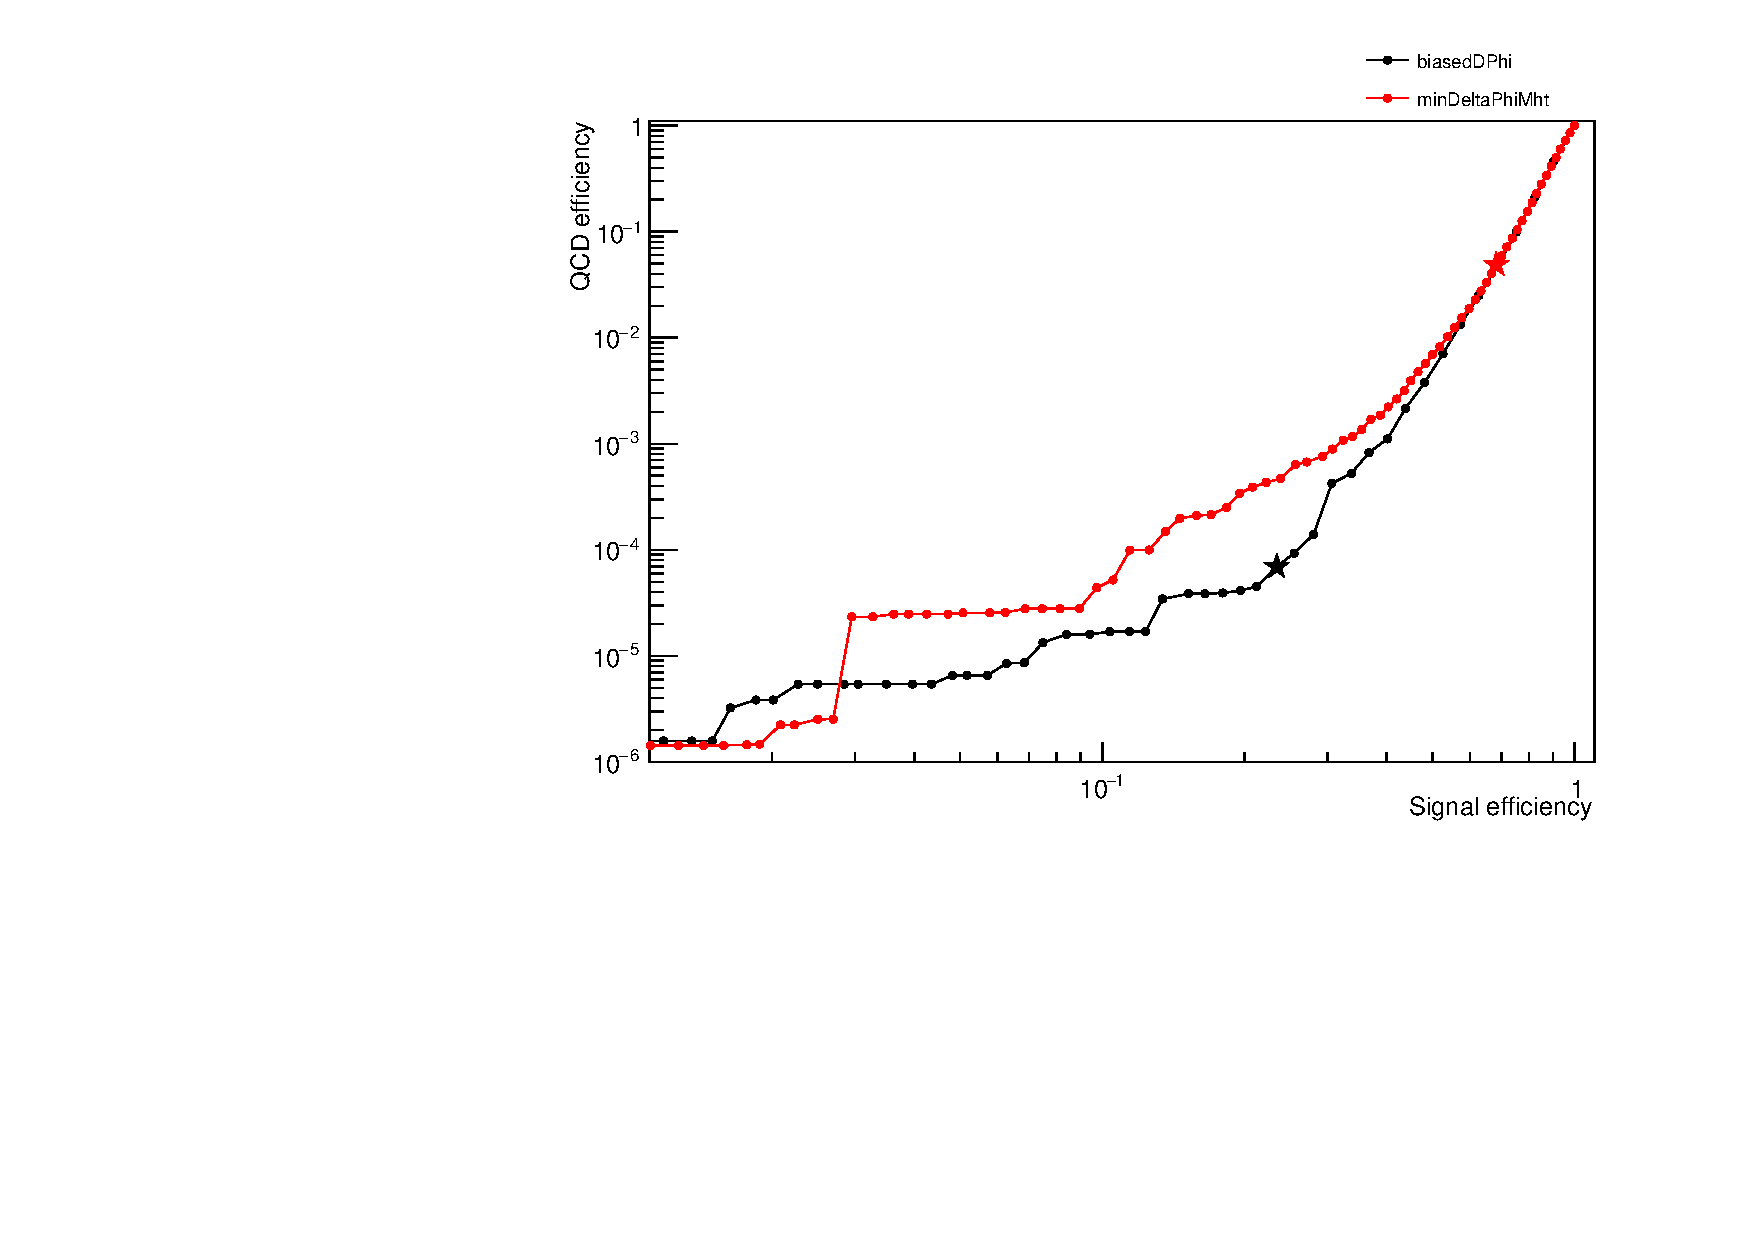
\includegraphics[width=0.5\textwidth]{figures/qcd/rateEffSignalQCD}
 } \\
 \caption{\bdphi, \dphimhtj and \dphimhtjall efficiency for simulation of processes with genuine
 \met vs QCD multijet background efficiency. The stars correspond to
 efficiencies with a cut of $0.5$ on each variable. A generic case of
 non-multijet process efficiency is considered in (a). In (b) we
 consider an uncompressed T1tttt model. This is the case in which \bdphi is
 expected to have the lowest efficiency due to the very high jet
 multiplicity of the model.}
 \label{fig:bDPhi_roc}
\end{figure}

\begin{figure}[!h]
 \centering
 \subfigure[QCD \bdphi distribution with mismeasurement.\label{fig:shifted_bDPhi_dist}]{
 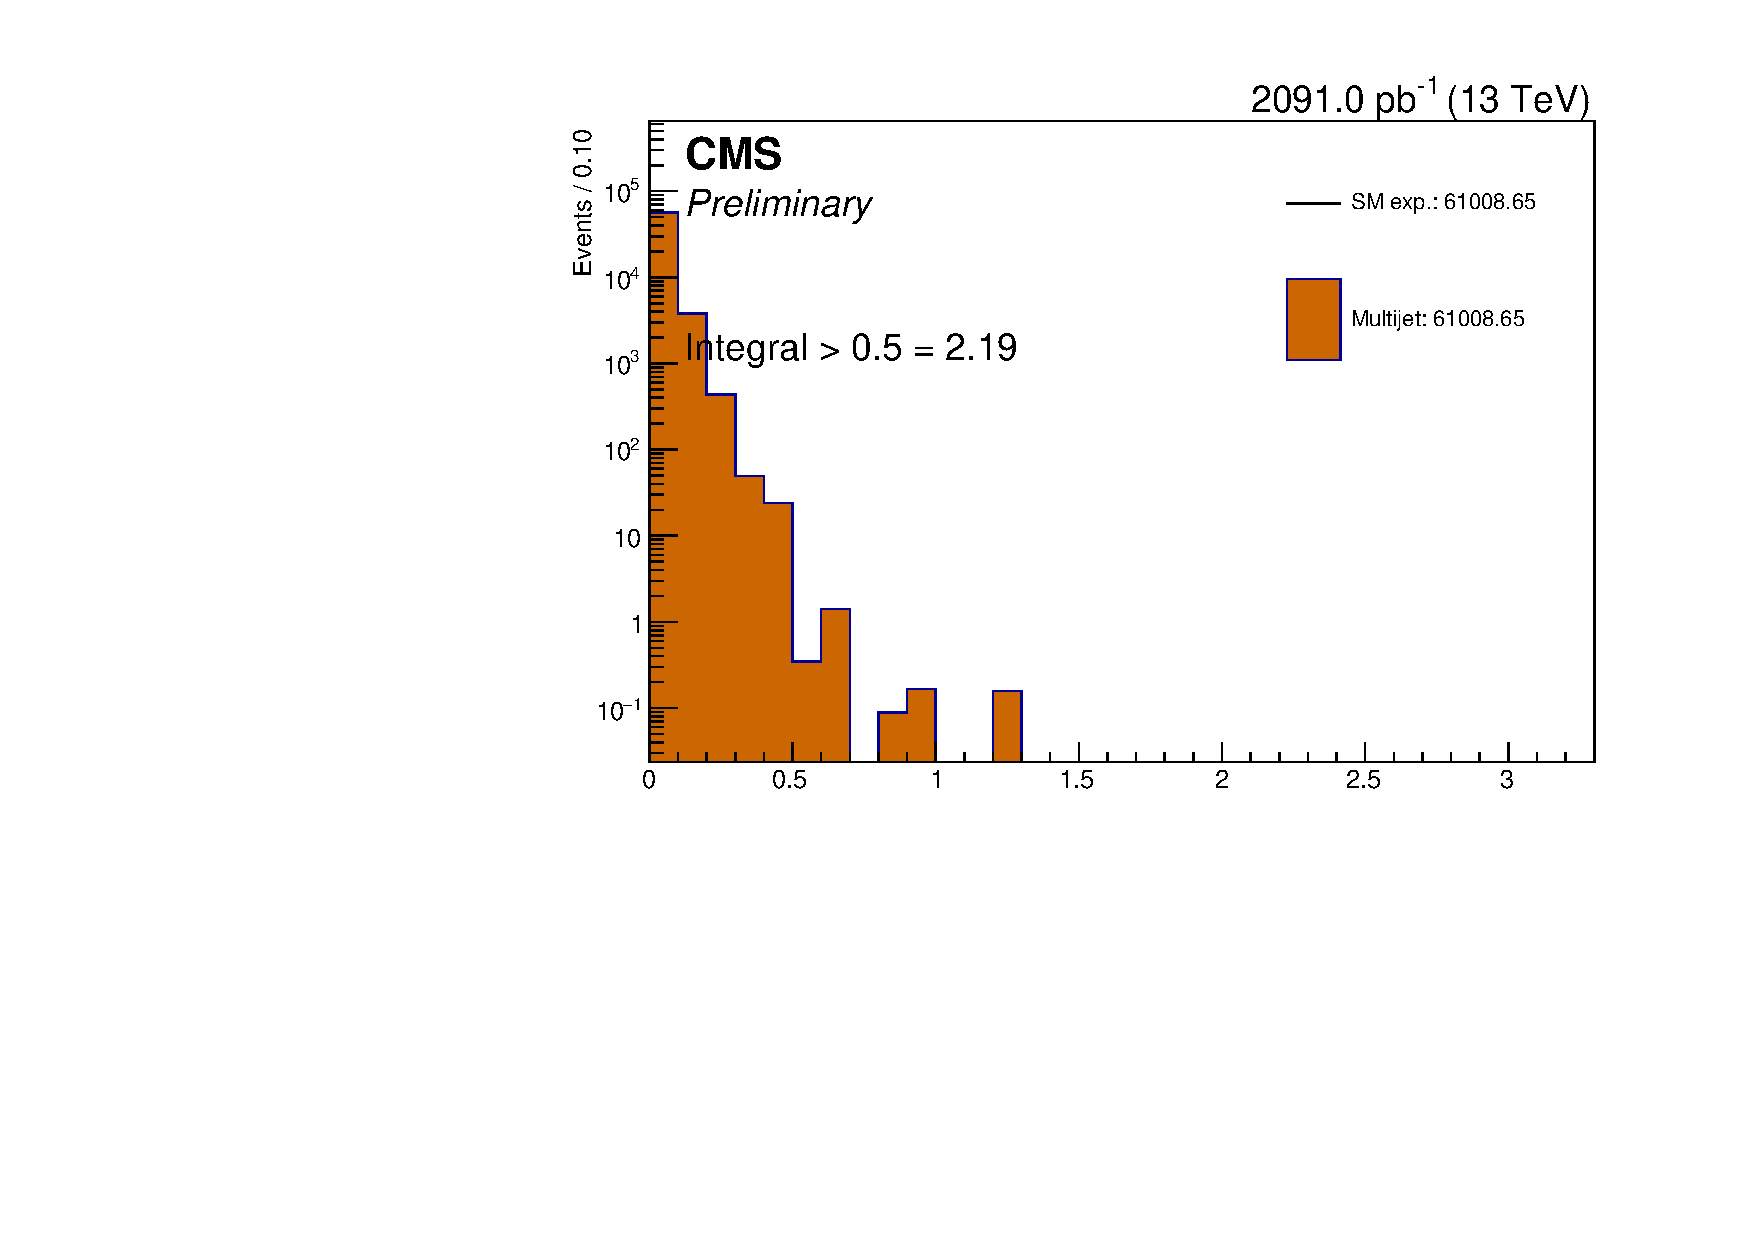
\includegraphics[width=0.5\textwidth]{figures/qcd/v6/bDPhi/shiftedMinBDPhi_all_800}
 }
 \subfigure[QCD \dphimhtj distribution with mismeasurement.\label{fig:shifted_DPhiMht_dist}]{
 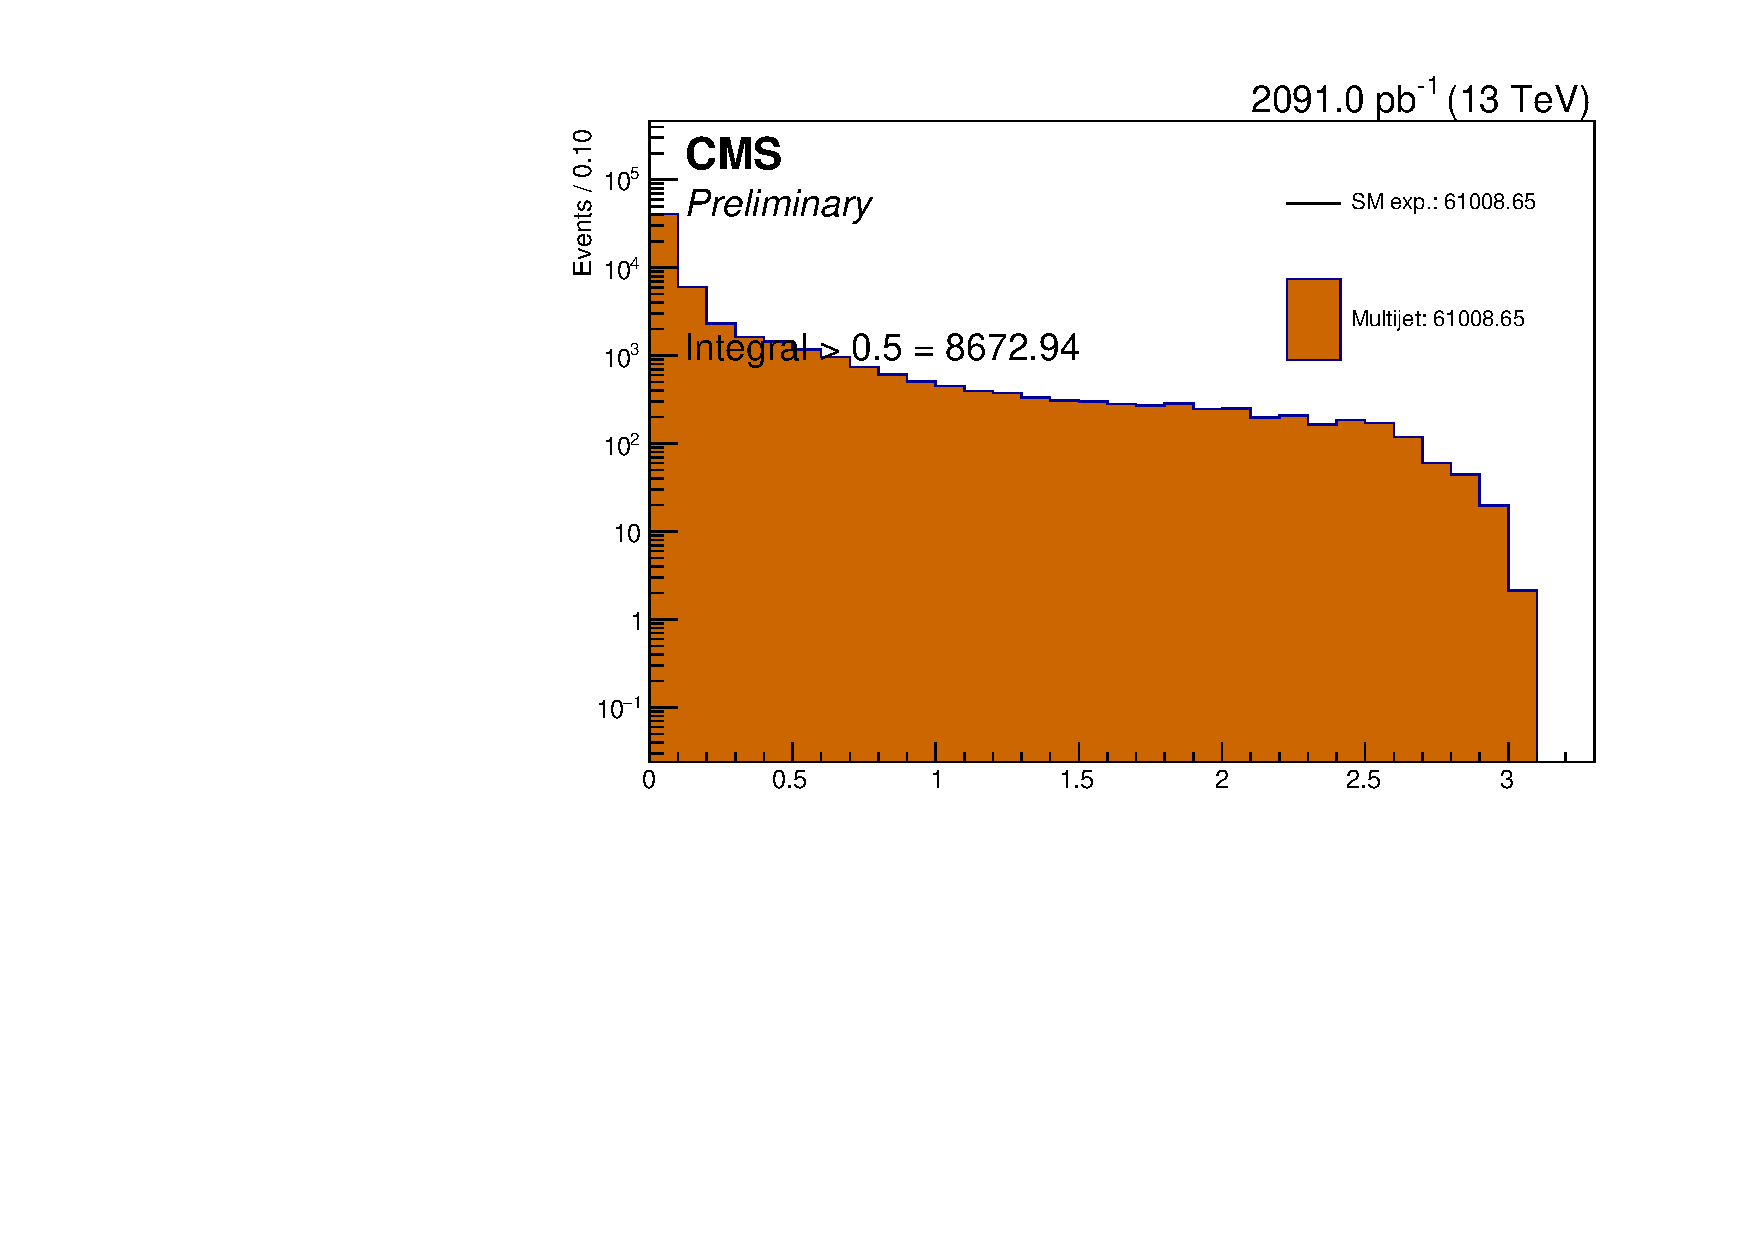
\includegraphics[width=0.5\textwidth]{figures/qcd/v6/bDPhi/shiftedMinDeltaPhiMht_all_800}
 } \\
 \caption{\bdphi and \dphimhtj distributions of QCD multijet simulation
 after analysis selections for \scalht $> 800$ \GeV in the case of
 severe mismeasurement. The
 total number of events that pass a $\Delta\phi > 0.5$ selection of the
 respective quantity are indicated. (N.B. these plots were made with
 an older iteration of the analysis and have not been fully updated,
 although their conclusions remain true)}
 \label{fig:bDPhi_mismeasured}
\end{figure}

\subsection{The method and results}
\label{sec:qcdMethod}

%FIXME Could reword this to remove the references to Run 1?
In Run~1, the \alphat and \bdphi thresholds that reduced
multijet contamination to the required level were determined by a
dedicated data-driven method, which relied on multijet-enriched
sidebands in the variables \alphat, \bdphi, and \mhtmet. The \mhtmet
variable, discussed in Sec.~\ref{sec:selection}, is used to filter QCD
multijet events that contain soft jets below threshold contributing
significantly to \mht. The method relied on extrapolating the
exponential modelling of the number of multijet events passing and
failing a requirement on the variable \mhtmet, \ie the pass/fail ratio
\rmhtmet, as a function of \alphat for a given signal region bin
(defined in terms of \njet, \nb, and \scalht). In essence, the
approach employed was an ABCD method that accounted for the
correlation between the variables \rmhtmet and \alphat, followed
by an additional requirement on \bdphi determined and validated in a
data control sideband.

For this search, we employ a simpler approach that relies on the
determination of the ratio \rmhtmet per (\njet,\scalht) bin from
simulation. The ratio is determined following the application of the
\alphat and \bdphi requirements, which in the former case are
\scalht-dependent. For the region $\scalht > 800\gev$, the requirement
$\mht > 130\gev$ is made in place of any on \alphat. No \alphat nor
\mht requirements are imposed for events in the monojet
category.\footnote{For events in the monojet bin, an implicit
  requirement of $\mht > 200\gev$ is indeed made given that $\mht =
  \scalht$ for monojet events. No \alphat calculation can be made
  given the absence of a second jet.} The requirements on \alphat,
\mht, and \bdphi as a function of \scalht are summarised in
Sec.~\ref{sec:selection}. 

Each ratio, \rmhtmet, is used as a
multiplier on the predicted QCD counts per (\njet,\scalht) bin in a
\mhtmet data sideband. 
These data counts are collected with the
\verb!HLT_HTxxx_AlphaT0pyy!  and \verb!HLT_HT800! signal triggers
described in Sec.~\ref{sec:triggers}. 

In order to obtain an estimate of the number
of QCD multijet events in the sideband, $\mathcal{Q}$, a maximum likelihood fit analagous to that
described in Sec.~\ref{sec:likelihood} is performed. In this
fit, the
electroweak backgrounds are determined with the method described in
Sec.~\ref{sec:ewk-method} with single muon, double muon
and single photon control regions that have the same selection as the control regions
described in Sec.~\ref{sec:selection}, apart from an inverted \mhtmet
cut. All relevant systematic uncertainties are taken into account,
including the shape uncertainties described in
Sec.~\ref{sec:mc-variations} and the data driven uncertainties
uncertainties described in Sec.~\ref{sec:closure-tests}. 
After the contribution of the electroweak backgrounds is
estimated, the
remaining data counts are attributed to QCD. In this prediction, all
counts and predictions are inclusive in \nb. The
product of these predicted QCD counts and the ratio, $\mathcal{Q} \times
\rmhtmet$, provides an estimate of the level of QCD multijet events in
each (\njet,\scalht) bin of the signal region. The estimate is
currently made inclusively with respect to the \nb\ and \mht for each
(\njet,\scalht) bin. 

\begin{figure}[!h]
  \centering
  \subfigure[Simulated QCD events in signal region.\label{fig:qcd_pass}]{
    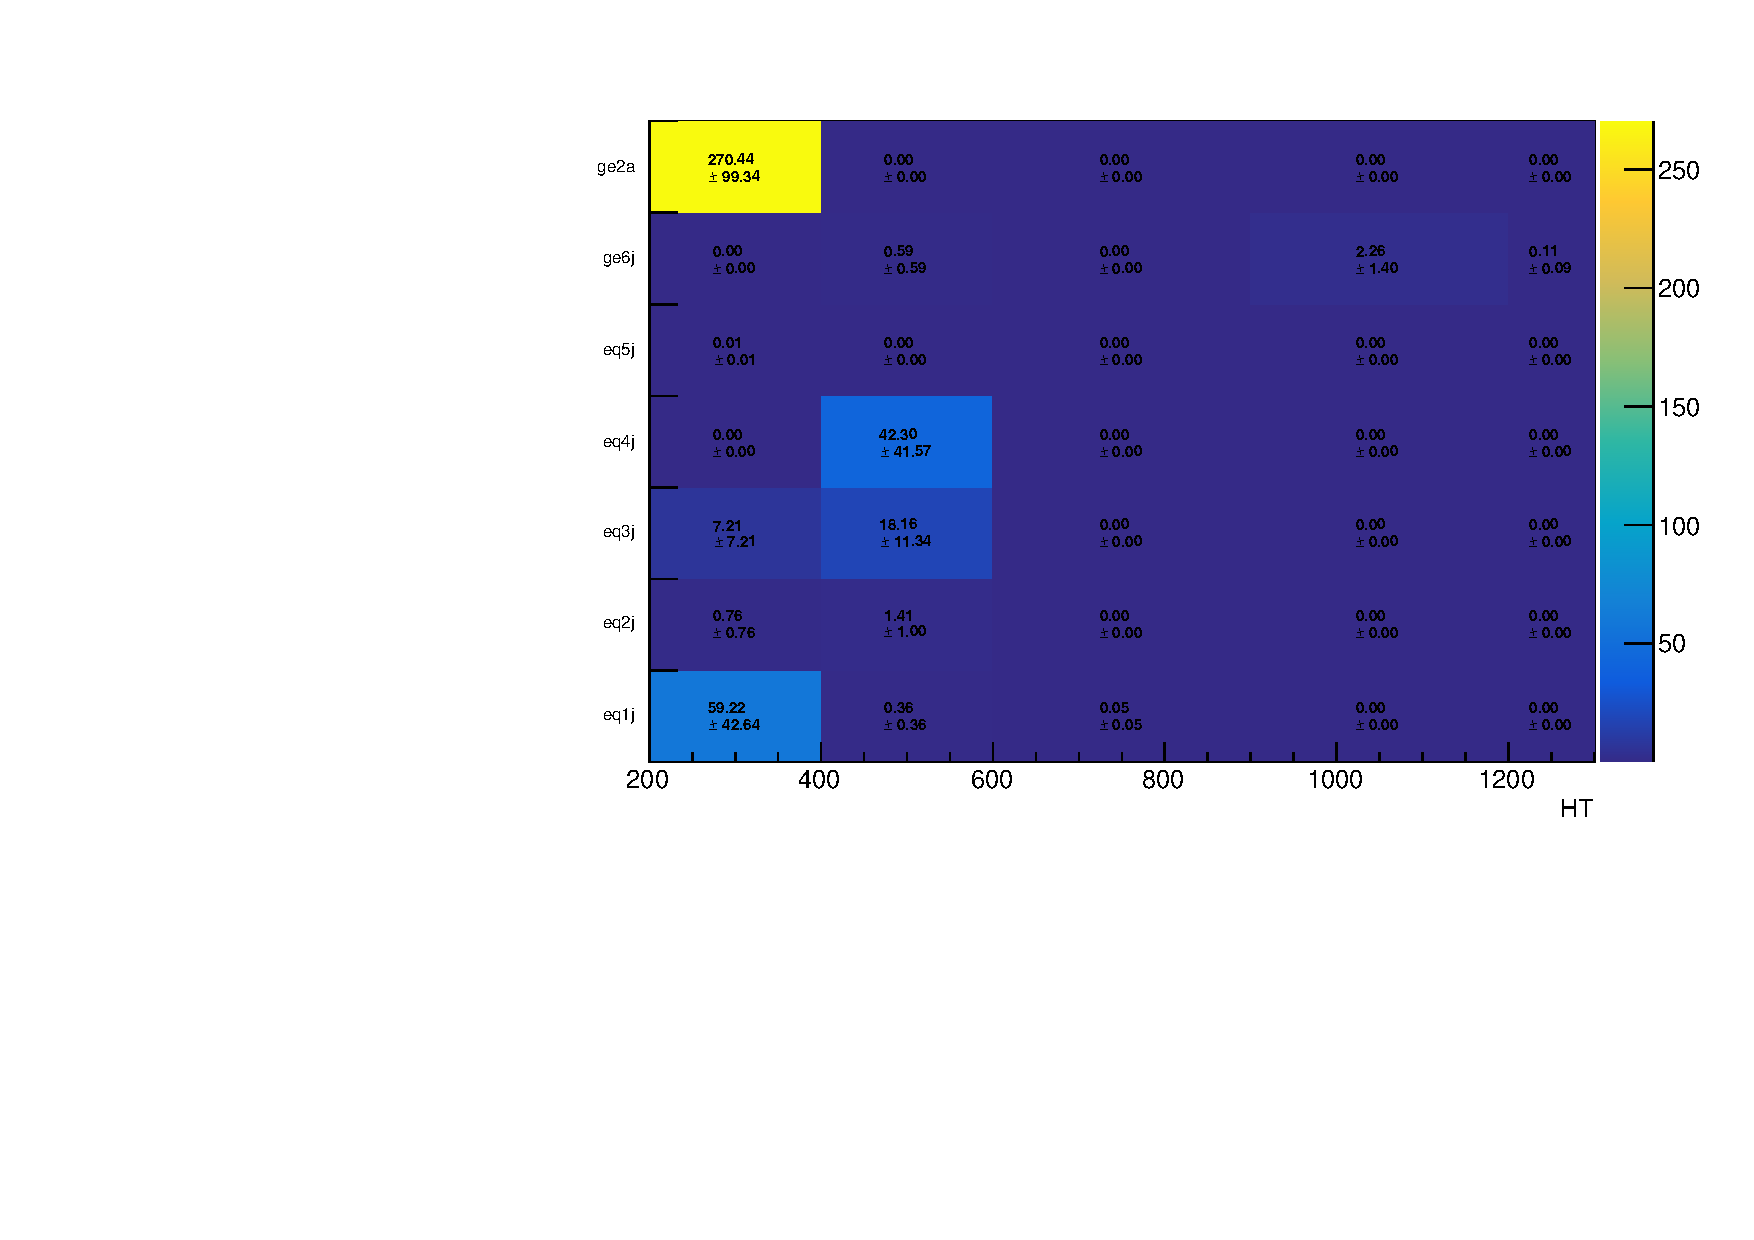
\includegraphics[width=0.5\textwidth]{figures/qcd/plots/signalQCD_MC}
  } 
  \subfigure[Simulated QCD events in \mhtmet sideband.\label{fig:qcd_fail}]{
    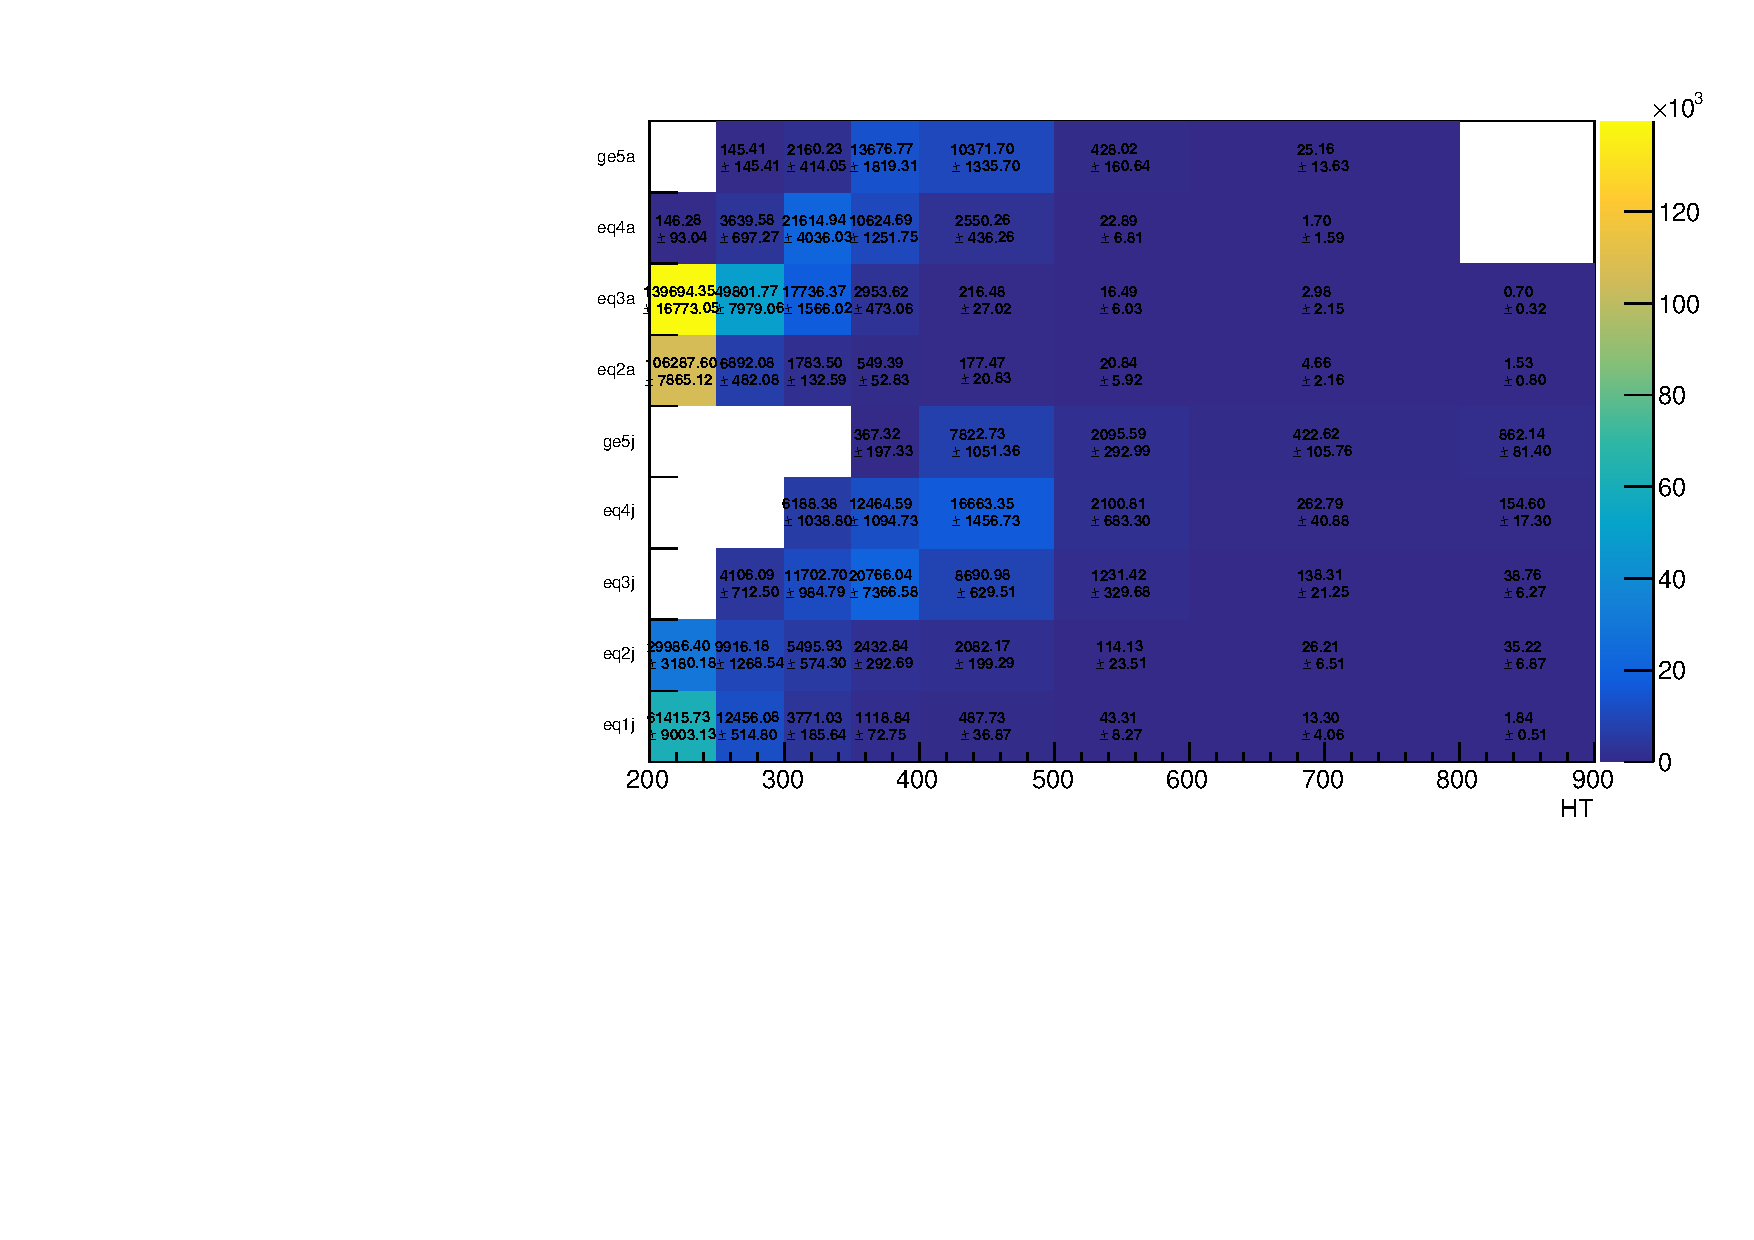
\includegraphics[width=0.5\textwidth]{figures/qcd/plots/qcdSbQCD_MC}
  } \\
  \subfigure[Ratio \rmhtmet for simulated QCD events.\label{fig:qcd_ratio}]{
    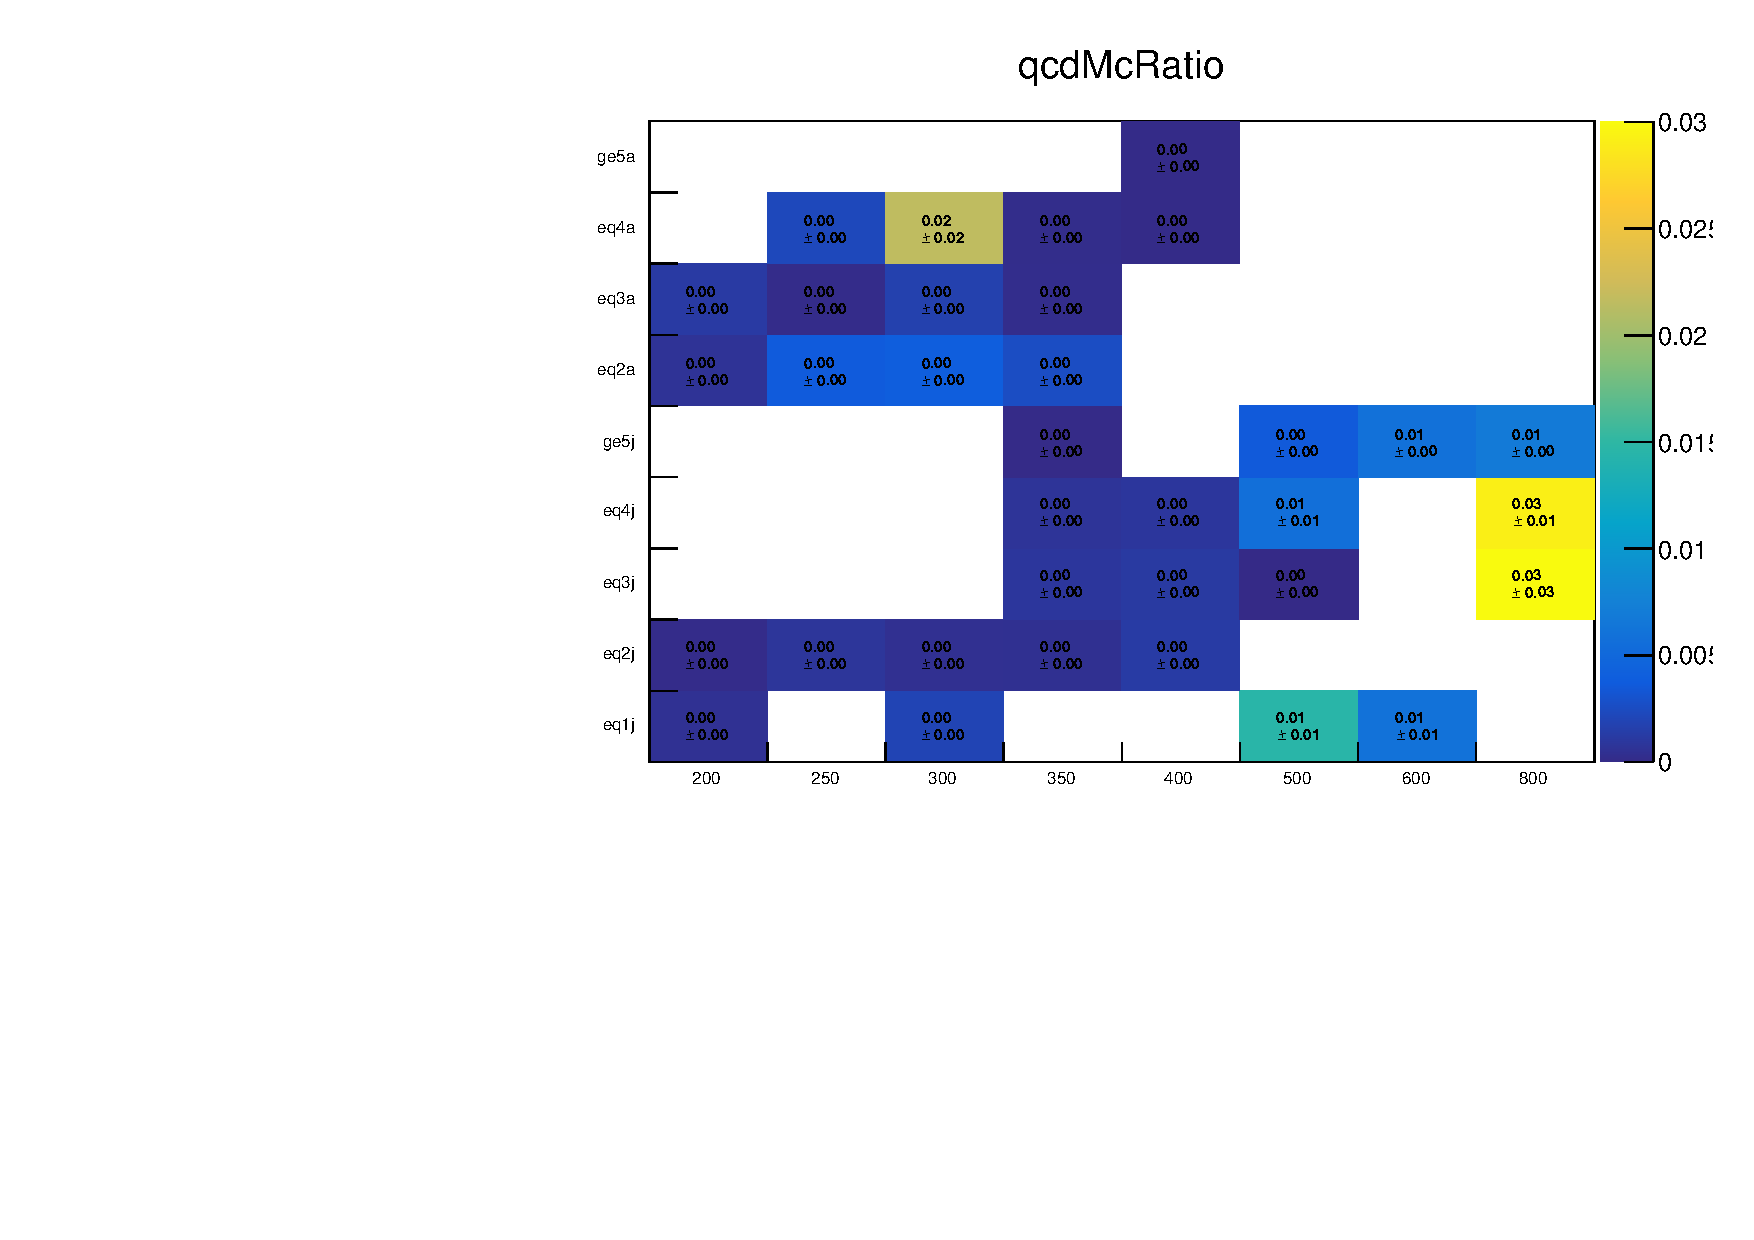
\includegraphics[width=0.5\textwidth]{figures/qcd/plots/signalQcdDivSbQcd_MC}
  } 
  \subfigure[Simulated EWK events in \mhtmet sideband.\label{fig:ewk_fail}]{
    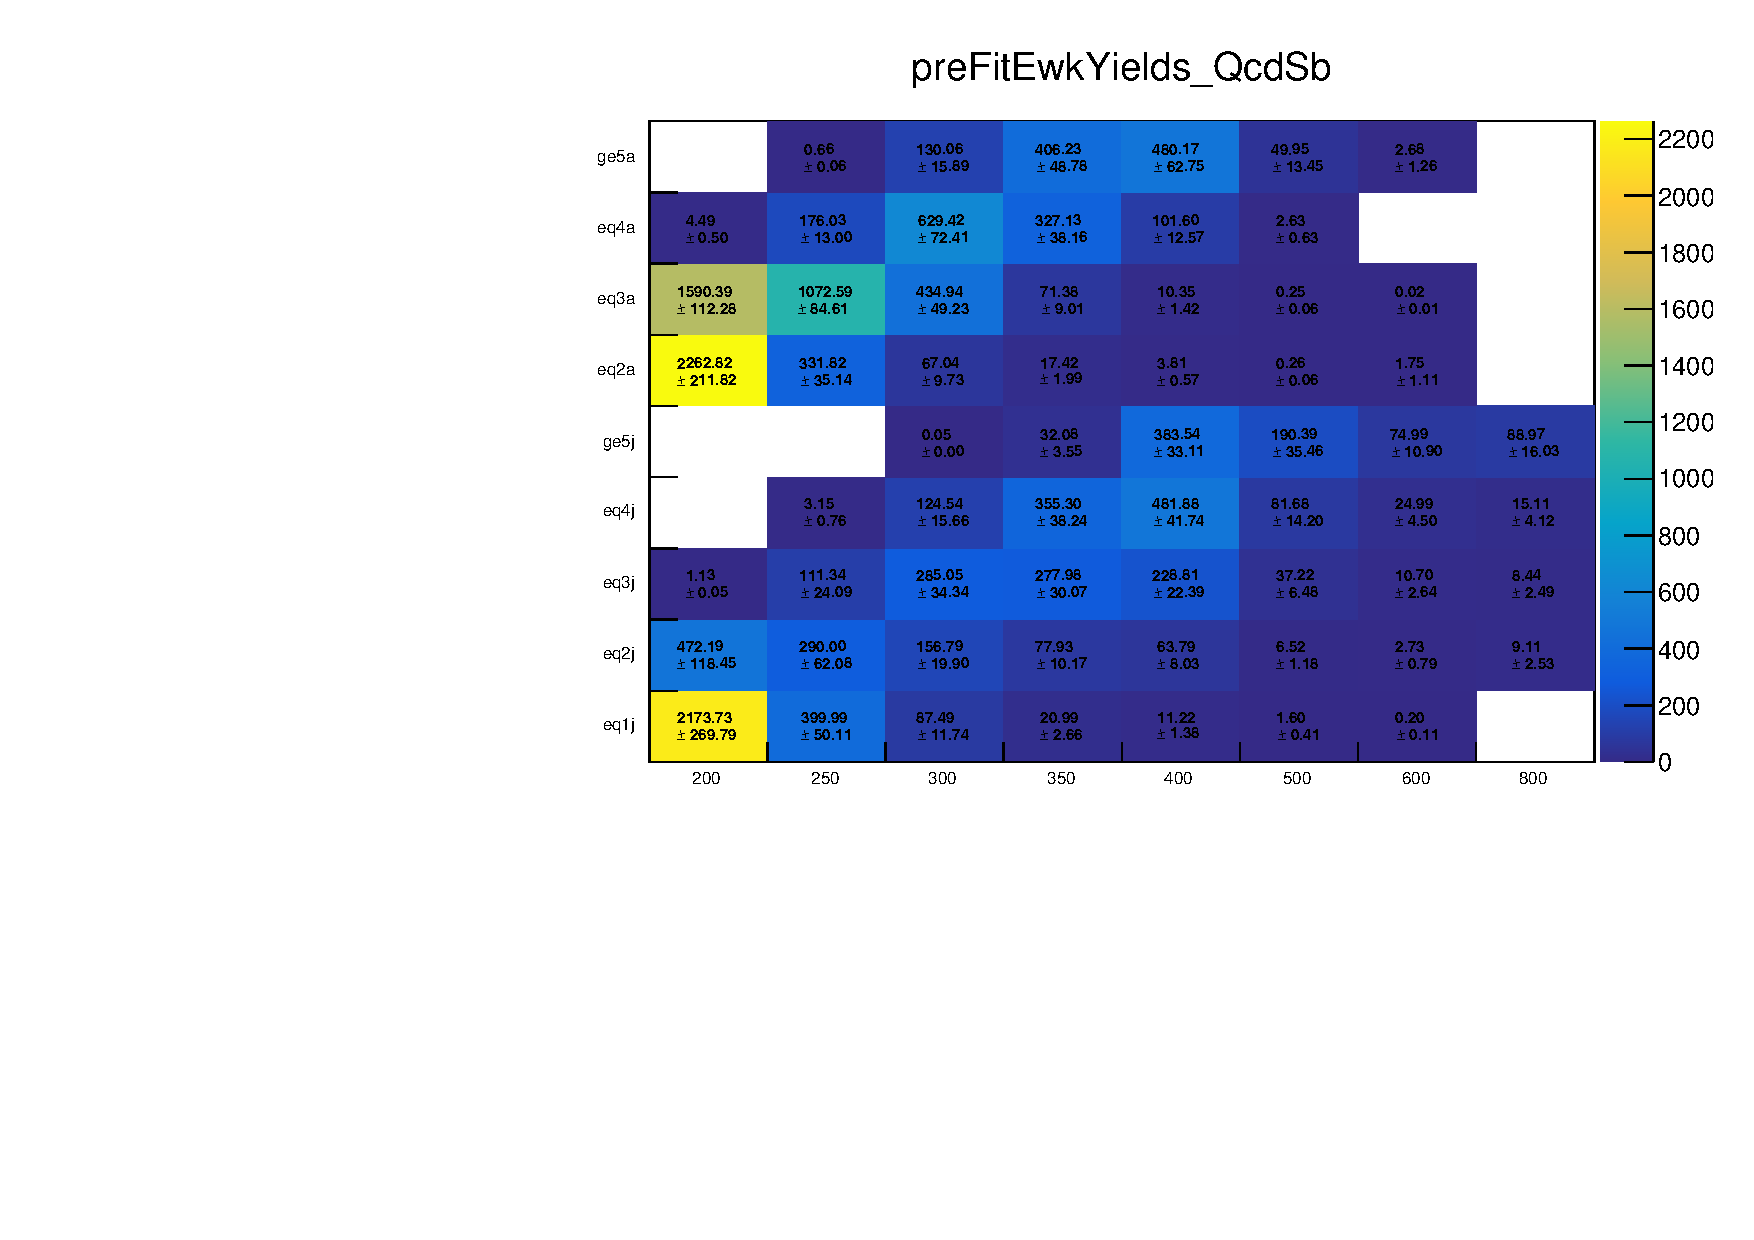
\includegraphics[width=0.5\textwidth]{figures/qcd/plots/qcdSbEwk_MC}
   %    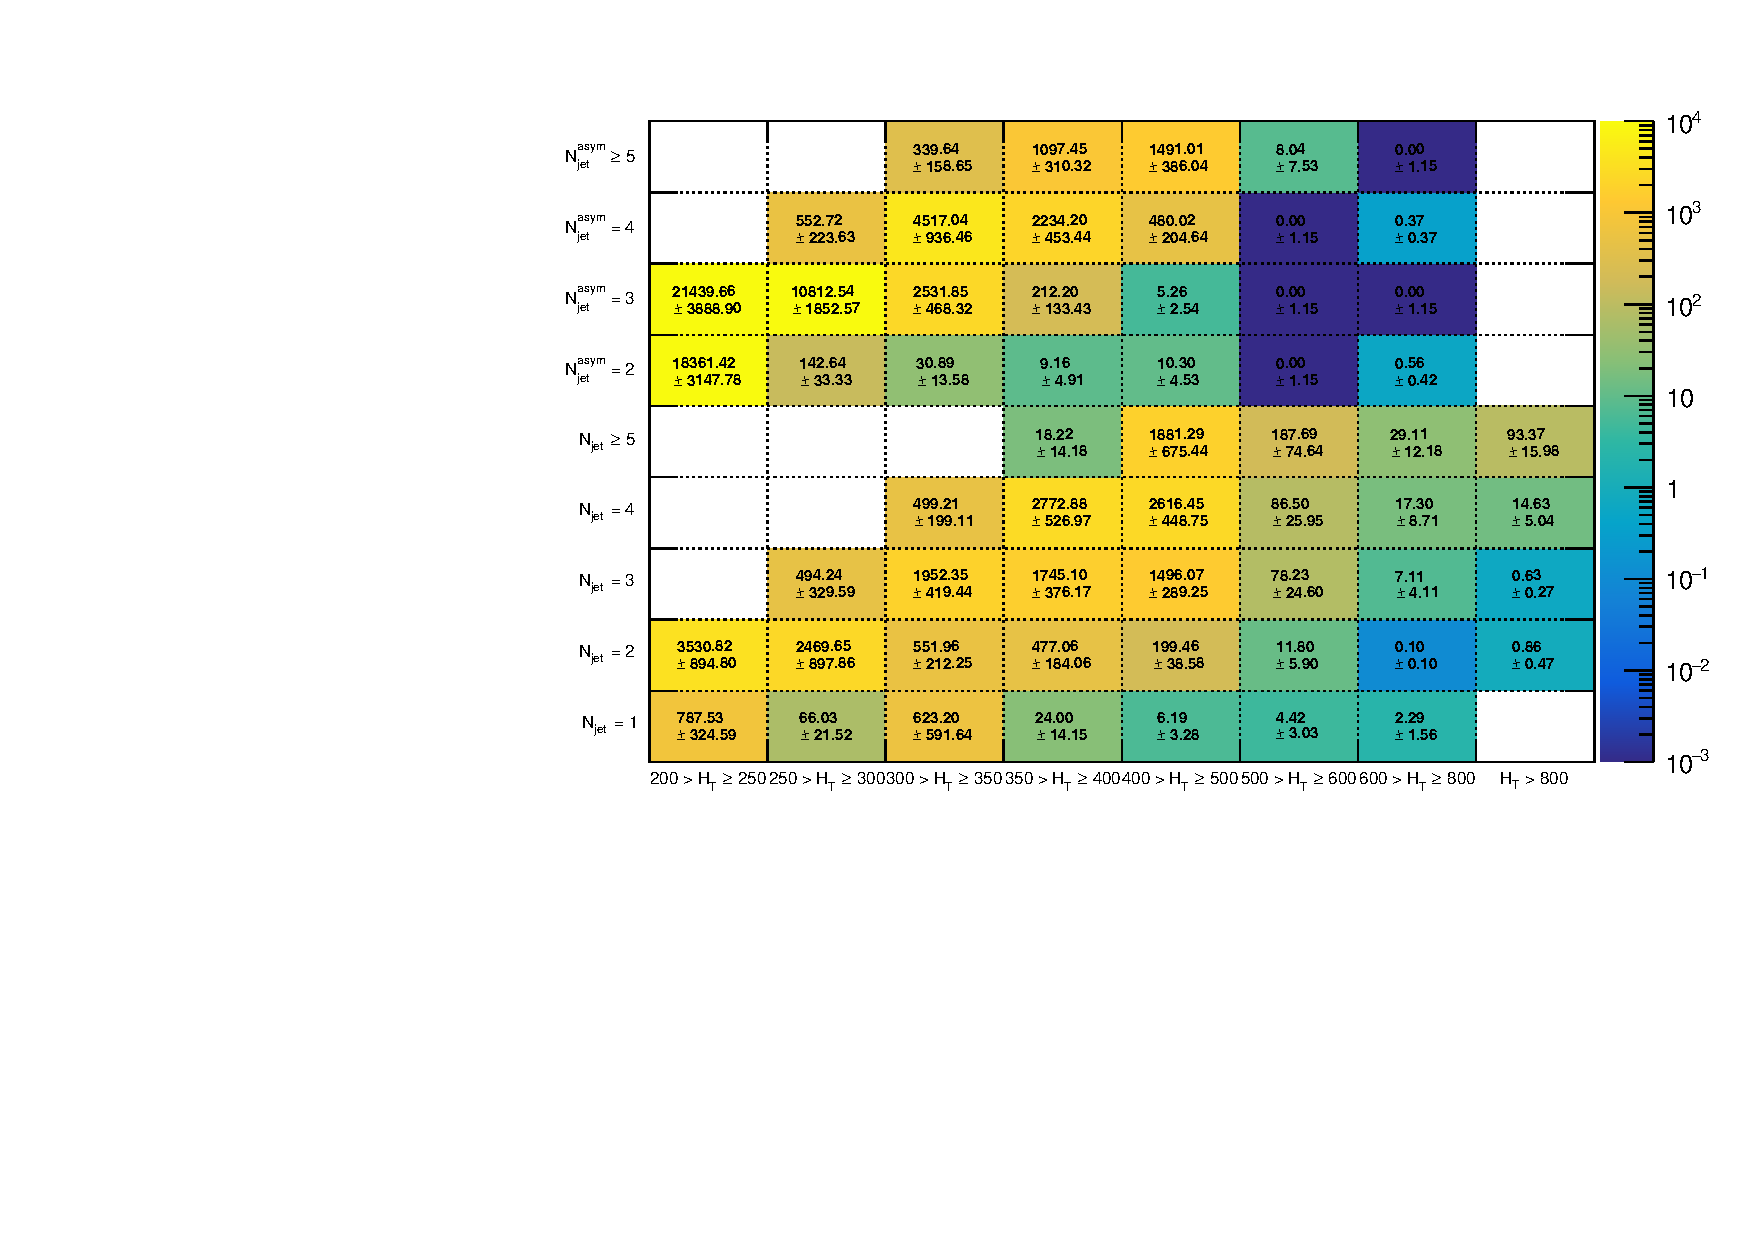
\includegraphics[width=0.5\textwidth]{figures/qcd/v6/Ewk/SigTrig_FailMoM_NJet_vs_HT_bDPhigt0p5_Log}
  } \\
  \caption{Expected number of QCD multijet events determined from
    simulation, binned according to \njet and \scalht, that (a) satisfy
    and (b) fail the requirement $\mhtmet < 1.25$. Also shown in (c)
    is the ratio \rmhtmet for QCD multijets, again determined from
    simulation. Finally, (d) shows the expected number of EWK events
    (V+jets and \ttbar, plus other residual non-multijet backgrounds)
    that fail the $\mhtmet < 1.25$ requirement, again determined from
    simulation and binned according to \njet and \scalht.}
  \label{fig:qcd_plots}
\end{figure}

The number of counts from multijet events satisfying and failing the
requirement $\mhtmet < 1.25$, \ie the pass/fail ratio \rmhtmet, are summarised in Fig.~\ref{fig:qcd_pass},
\ref{fig:qcd_fail}, and \ref{fig:qcd_ratio}. Figure~\ref{fig:ewk_fail}
shows the expected counts from non-multijet backgrounds in the \mhtmet
sideband, as determined from simulation.

\begin{figure}[!h]
  \centering
  \subfigure[Binned data counts in \mhtmet sideband.\label{fig:data_fail}]{
    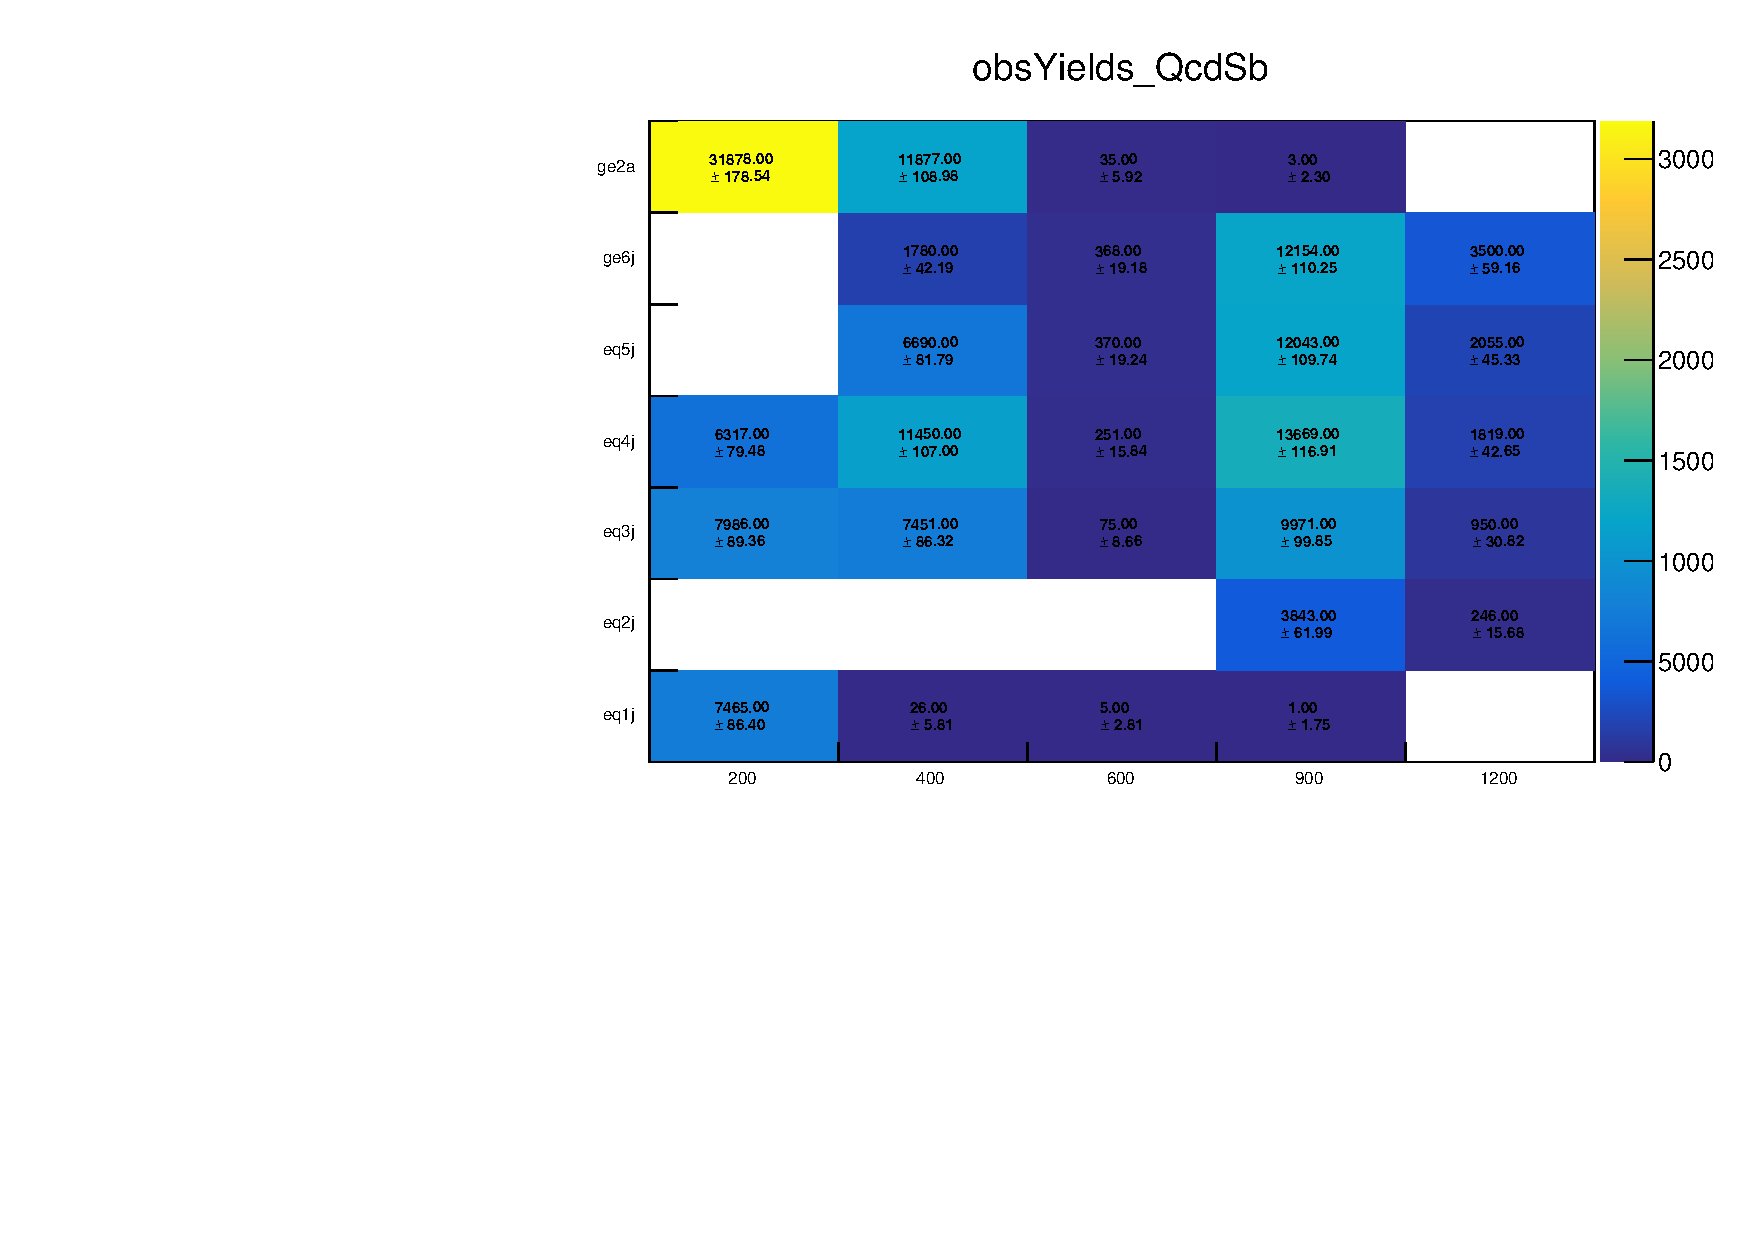
\includegraphics[width=0.5\textwidth]{figures/qcd/plots/obsYields_QcdSb}
  } 
  \subfigure[Predicted QCD counts in \mhtmet sideband.\label{fig:data_corr}]{
    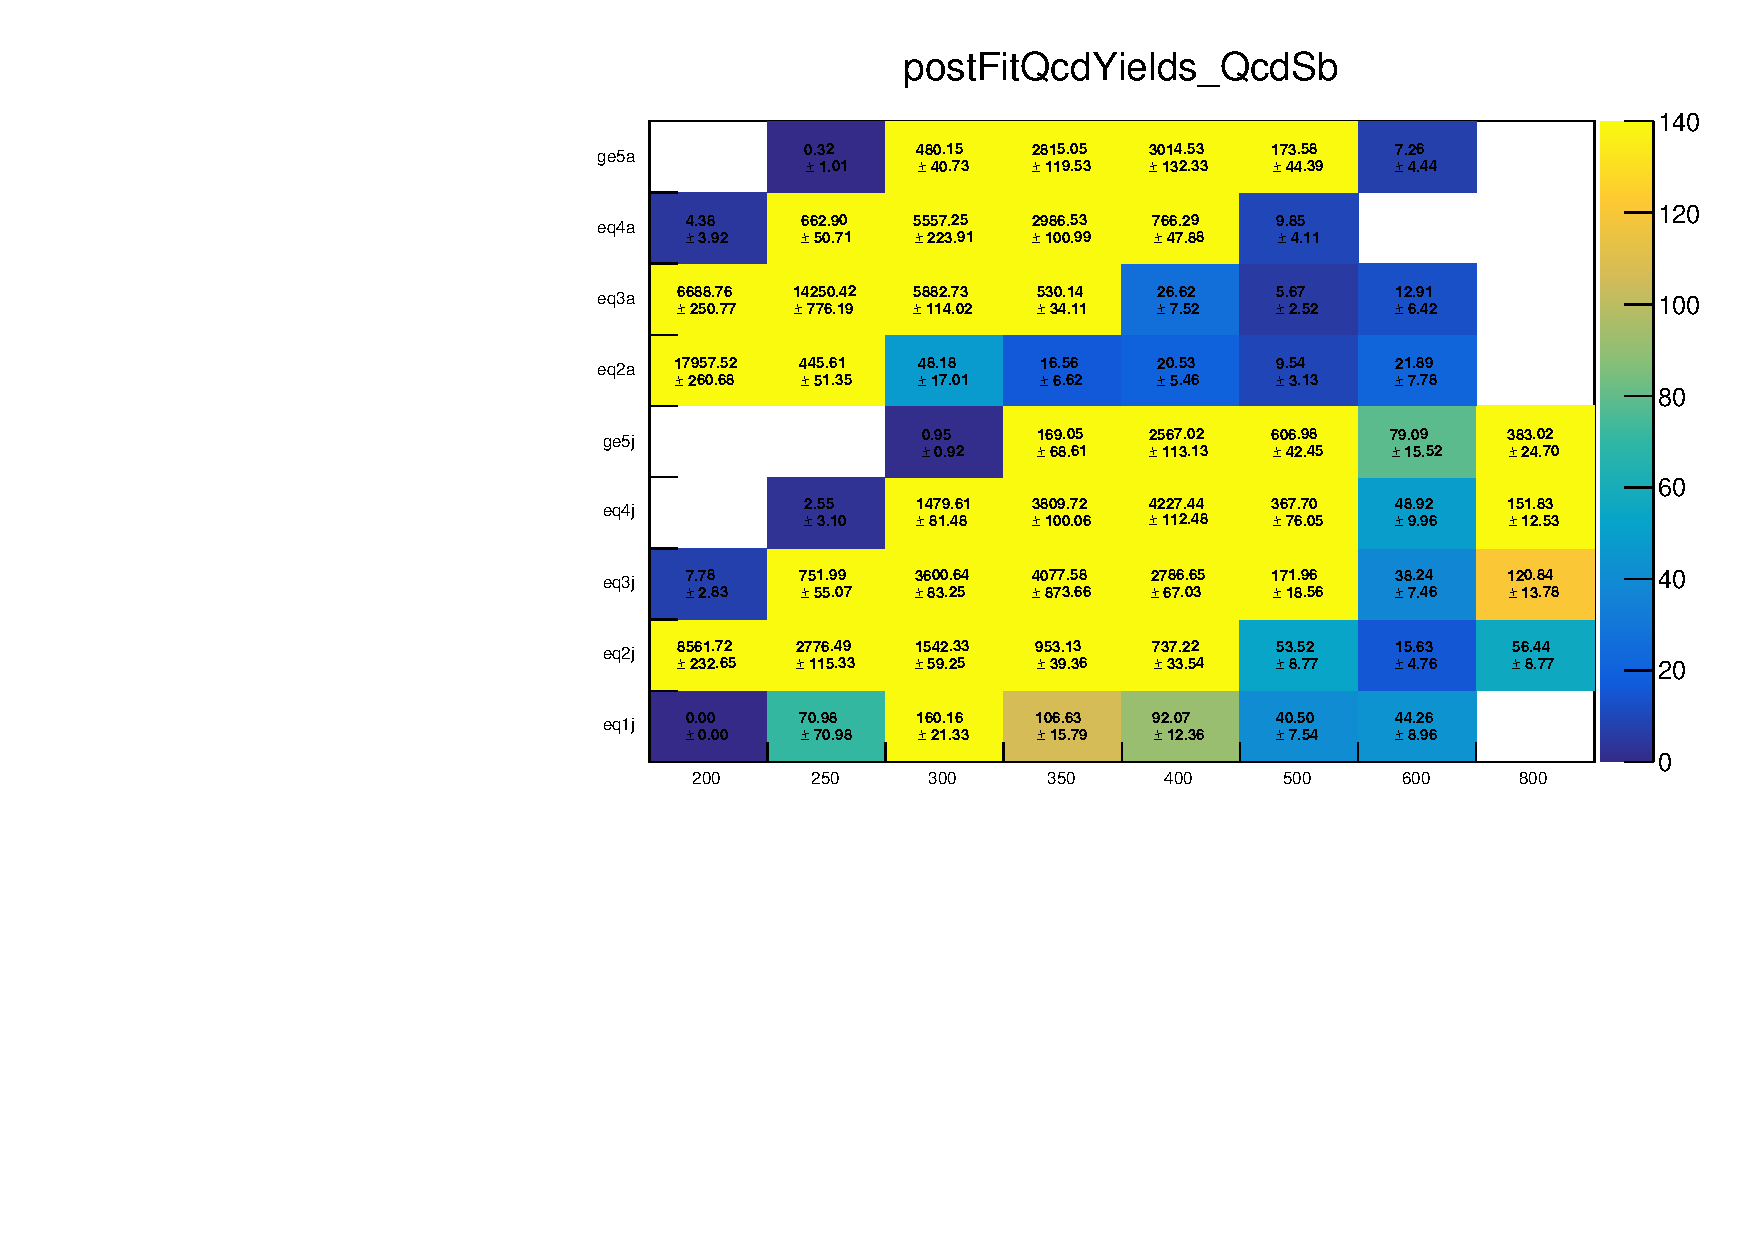
\includegraphics[width=0.5\textwidth]{figures/qcd/plots/postFitQcdYields_QcdSb}
  } \\
  \subfigure[QCD multijet predictions in the signal region.\label{fig:qcd_pred}]{
    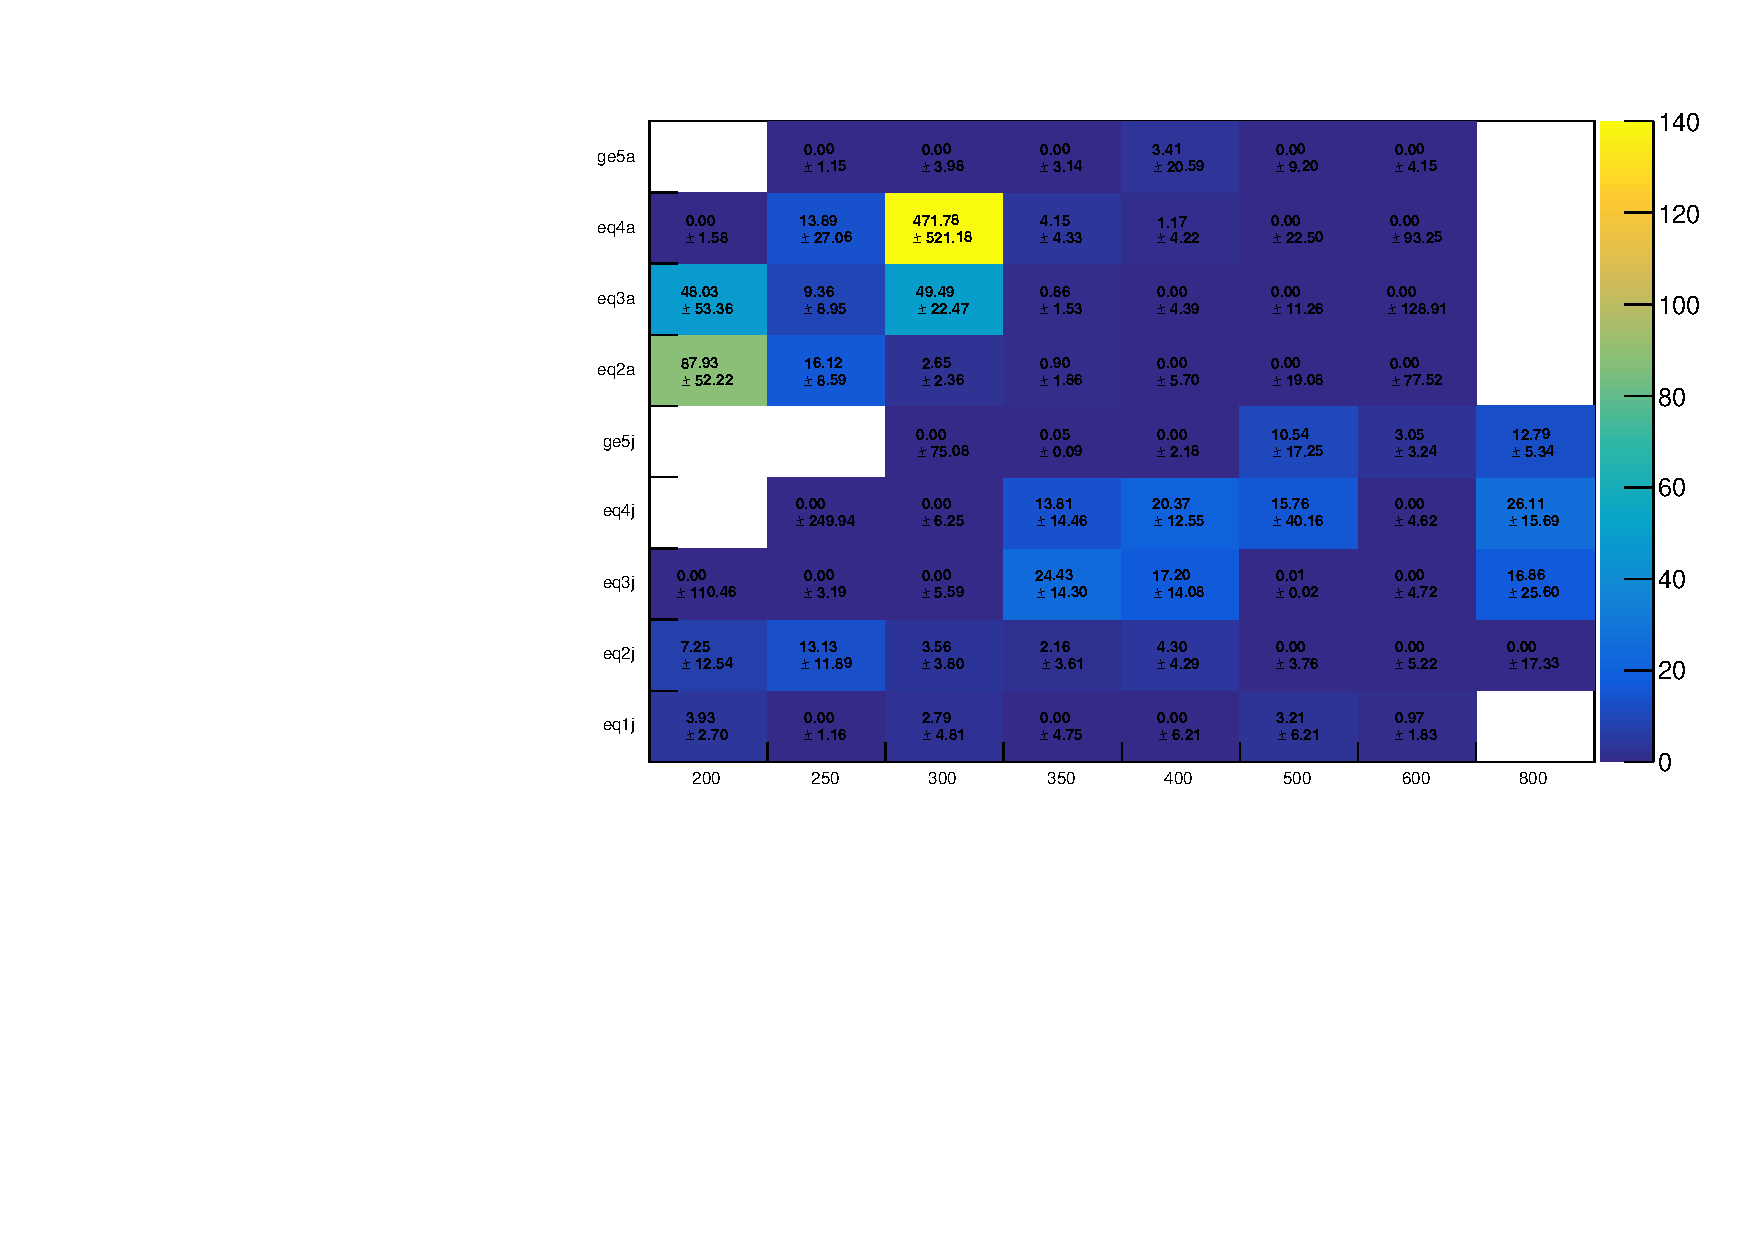
\includegraphics[width=0.5\textwidth]{figures/qcd/plots/predictedQcdYields_Signal}
  } 
  \subfigure[Ratio of predicted multijet and non-multijet yields.\label{fig:qcd_ewk_ratio}]{
    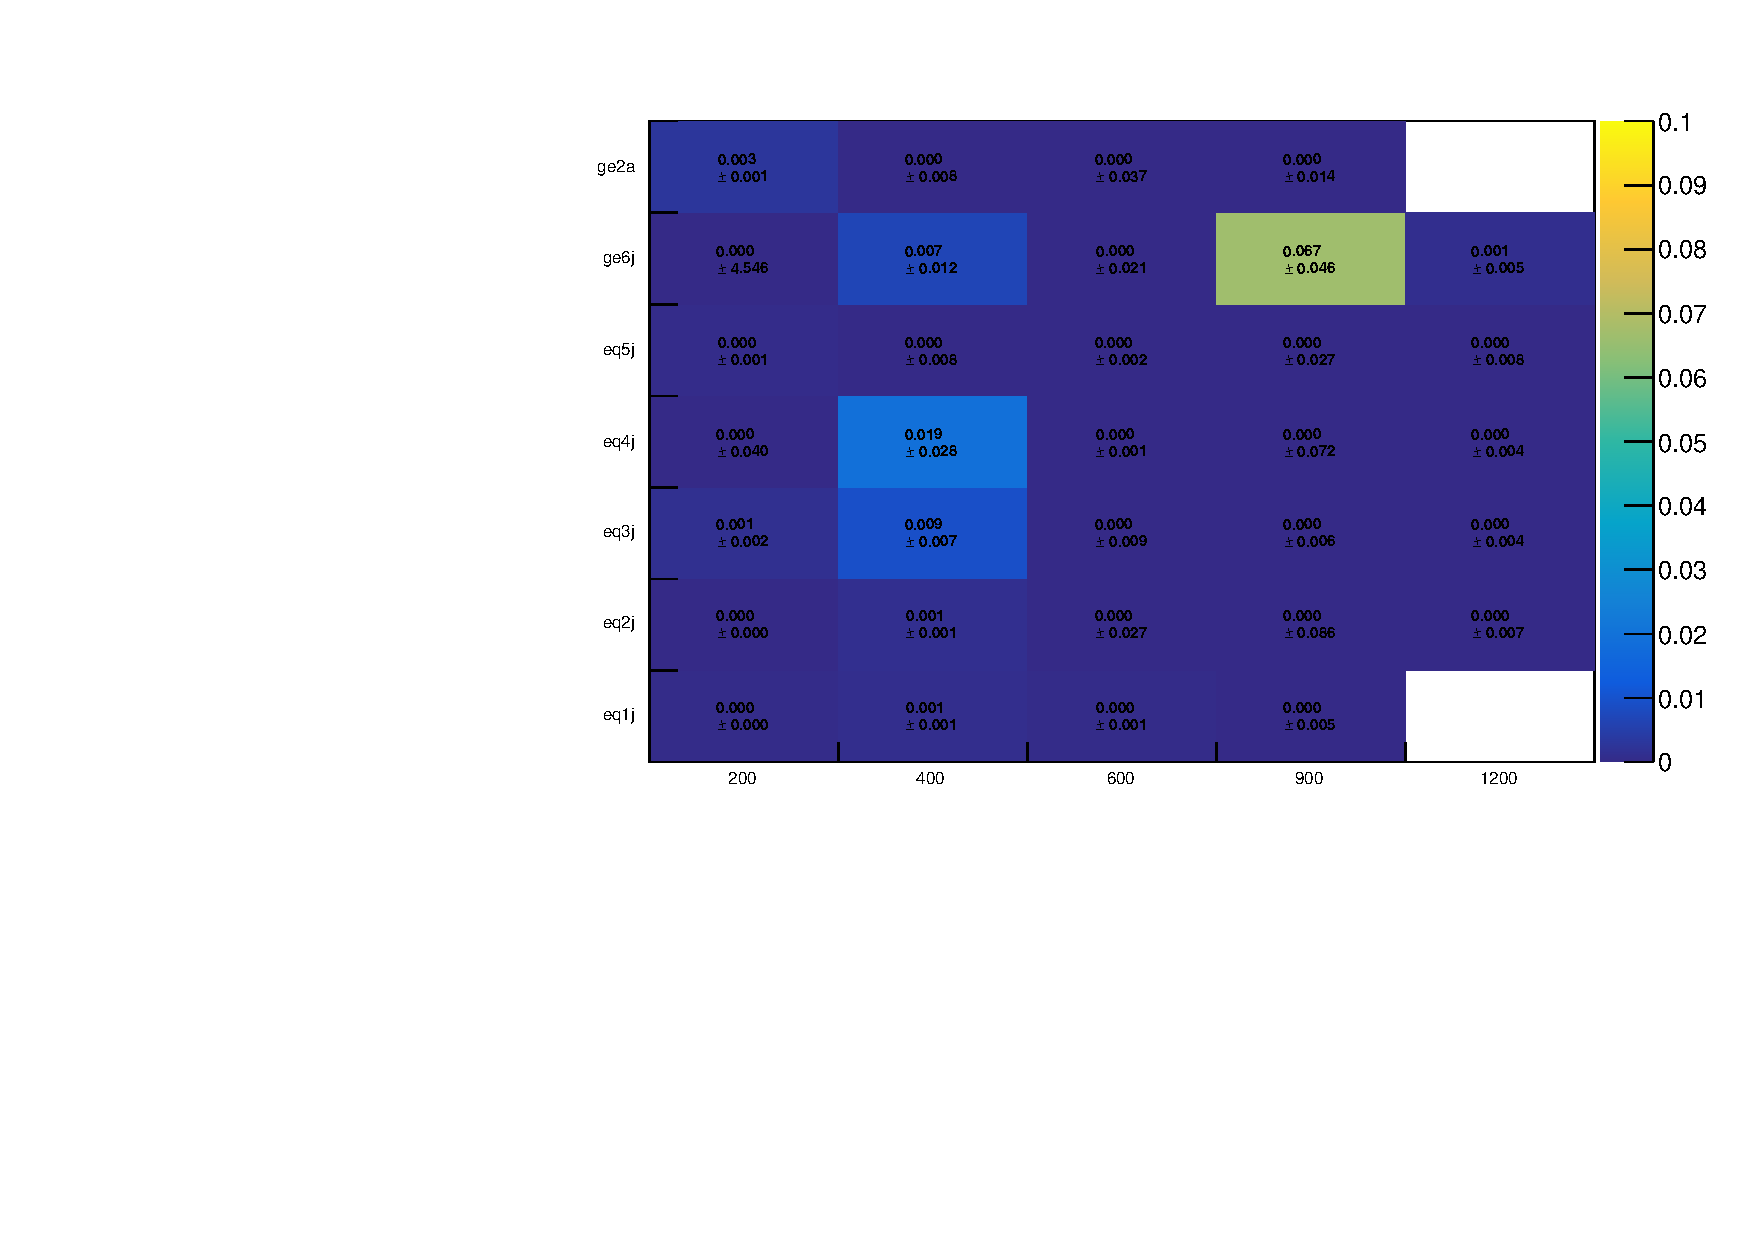
\includegraphics[width=0.5\textwidth]{figures/qcd/plots/predictedQcdDivEwk_Signal}
  } \\
  \caption{The number of events observed in the $\mhtmet>1.25$ sideband, 
    binned according to \njet and \scalht are shown in (a). In
    (b) these yields are corrected by subtracting the expected
    electroweak component. Shown in
    (c) is the result of multiplying the observed multijet events predicted
    in (b) by the translation factor from the sideband to the signal
    region determined with simulation (shown in
    Fig.~\ref{fig:qcd_plots}). This gives a data driven expectation of
    the quantity of multijet background events in the signal region. 
    Finally, (d), shows the ratio of expected
    multijet background events in the signal region divided by
    non-multijet backgrounds. The multijet background is therefore
    shown to be at the percent level.}
  \label{fig:qcd_plots2}
\end{figure}

% THIS IS NOW UNNECESSARY:  
% The data counts in the \mhtmet sideband are collected with the
% \verb!HLT_HTxxx_AlphaT0pyy!  and \verb!HLT_HT800! signal triggers
% described in Sec.~\ref{sec:triggers}. Events satisfy the full signal
% region requirements plus the inverted \mhtmet requirement and are
% binned according to \njet and \scalht. 
% Any contribution from
% non-multijet backgrounds (V+jets, \ttbar, \etc) in each bin is
% estimated from simulation\footnote{In the future, the counts from
%   non-multijet backgrounds will be estimated from the muon data
%   control samples and transfer factors determined from simulation
%   (using the method described in Sec.~\ref{sec:backgroundmet}).} and
% subtracted from the data counts. Any remaining counts, $\mathcal{Q}$,
% are assumed to arise from multijet production.
Figure~\ref{fig:data_fail} shows the observed counts in the \mhtmet
sideband, and Fig.~\ref{fig:data_corr} shows the QCD counts 
in the sideband predicted by the maximum likelihood fit.
Figure~\ref{fig:qcd_pred} shows the predicted counts for the multijet
contribution in the signal region bins, which are obtained from the
products of \rmhtmet and $\mathcal{Q}$, summarised in
Figs.~\ref{fig:qcd_ratio} and \ref{fig:data_corr}. Finally,
Fig.~\ref{fig:qcd_ewk_ratio} shows the ratios of predicted multijet
counts with respect to the expected EWK counts in the signal region.
This allows the quantification of
the (predicted) relative contamination from multijet events in the
signal region bins. The EWK \mht and \nb shapes derived from
simulation are used to predict the distribution 
of QCD events, this approach is validated in
Sec.~\ref{sec:qcdValidation}. 

%% The predictions summarised in Fig.~\ref{fig:qcd_ewk_ratio} support the
%% expectation based on experience with 8~TeV data that the \HT-dependent
%% \alphat thresholds defined in Table~\ref{tab:sr-selections} and the
%% requirement of $\bdphi > 0.5$ are sufficient to reduce the multijet
%% contamination in all bins of the signal region to the sub-percent with
%% respect to the total non-multijet background. With this level of
%% suppression, it is expected that the uncertainty associated with the
%% residual multijet contamination to be sub-dominant with respect to,
%% and fully absorbed by, the systematic uncertainties on the non-multijet
%% backgrounds, which are expected to be at the level of $\sim$10\% or
%% larger. 

The predictions summarised in Fig.~\ref{fig:qcd_ewk_ratio} show that 
the \HT-dependent \alphat thresholds defined in Table~\ref{tab:sr-selections} 
and the requirement of $\bdphi > 0.5$ suppress the multijet
contamination in all bins of the signal region to percent-level or smaller with
respect to the total non-multijet background. These predicted multijet events are 
included as a background contribution to the likelihood model
described in Sec~\ref{sec:likelihood}.

\subsubsection{Reduction in predicted QCD yields}

The
total number of QCD events predicted in the signal region has consistently
reduced across all analysis bins with respect to the 2015 analysis. The major difference that has led to
this change is an update in the QCD MC.
In the 2015 analysis, and early iterations of the 2016 analysis,
QCD MC reconstructed with version 74X of CMSSW was used. The update to
the
analysis, detailed in this note, uses QCD MC that is reconstructed with the 80X
version of CMSSW. With this update there was a significant
change in the modelling of the \mhtmet distribution,
demonstrated in Fig.~\ref{fig:mhtDivMetChange}. In the 80X QCD MC
only 0.4\% of the QCD events pass the 1.25 \mhtmet cut made on the
signal region. In the 74X MC, however, 1.6\% of the QCD events pass.
Unlike for the QCD multijet background, the cut efficiency for the 
non-multijet Standard Model backgrounds is
consistently $\sim 90\%$. As the non-multijet backgrounds are dominant
in the signal region, this results in a small change to the total
prediction in the signal region, despite there being a factor $\sim 4$
change to the predicted QCD. The effects of the \mhtmet mismodelling
on the non-multijet background prediction (described in Sec.~\ref{sec:backgroundmet})
is mitigated by the application of the cut across all control regions.

The QCD MC that passes selection typically consists of a few events
with very high weights, resulting in a large statistical
uncertainty. This leads to a large uncertainty on the total QCD
prediction with the method described in this section. Therefore,
despite the 2016 application of the method predicting less QCD in the
signal region,
the prediction in each bin is still statistically compatible with that  
made in 2015. 

In the parked data analysis of 8\tev data, the level of QCD
contamination was much lower than that seen
in 2015. With the change in the QCD simulation, predictions
more compatible with those seen in Run~1 are observed.

\begin{figure}[!h]
  \centering
  % \subfigure[\mhtmet distributions in the signal region with 74X QCD
  % MC.]{
  %   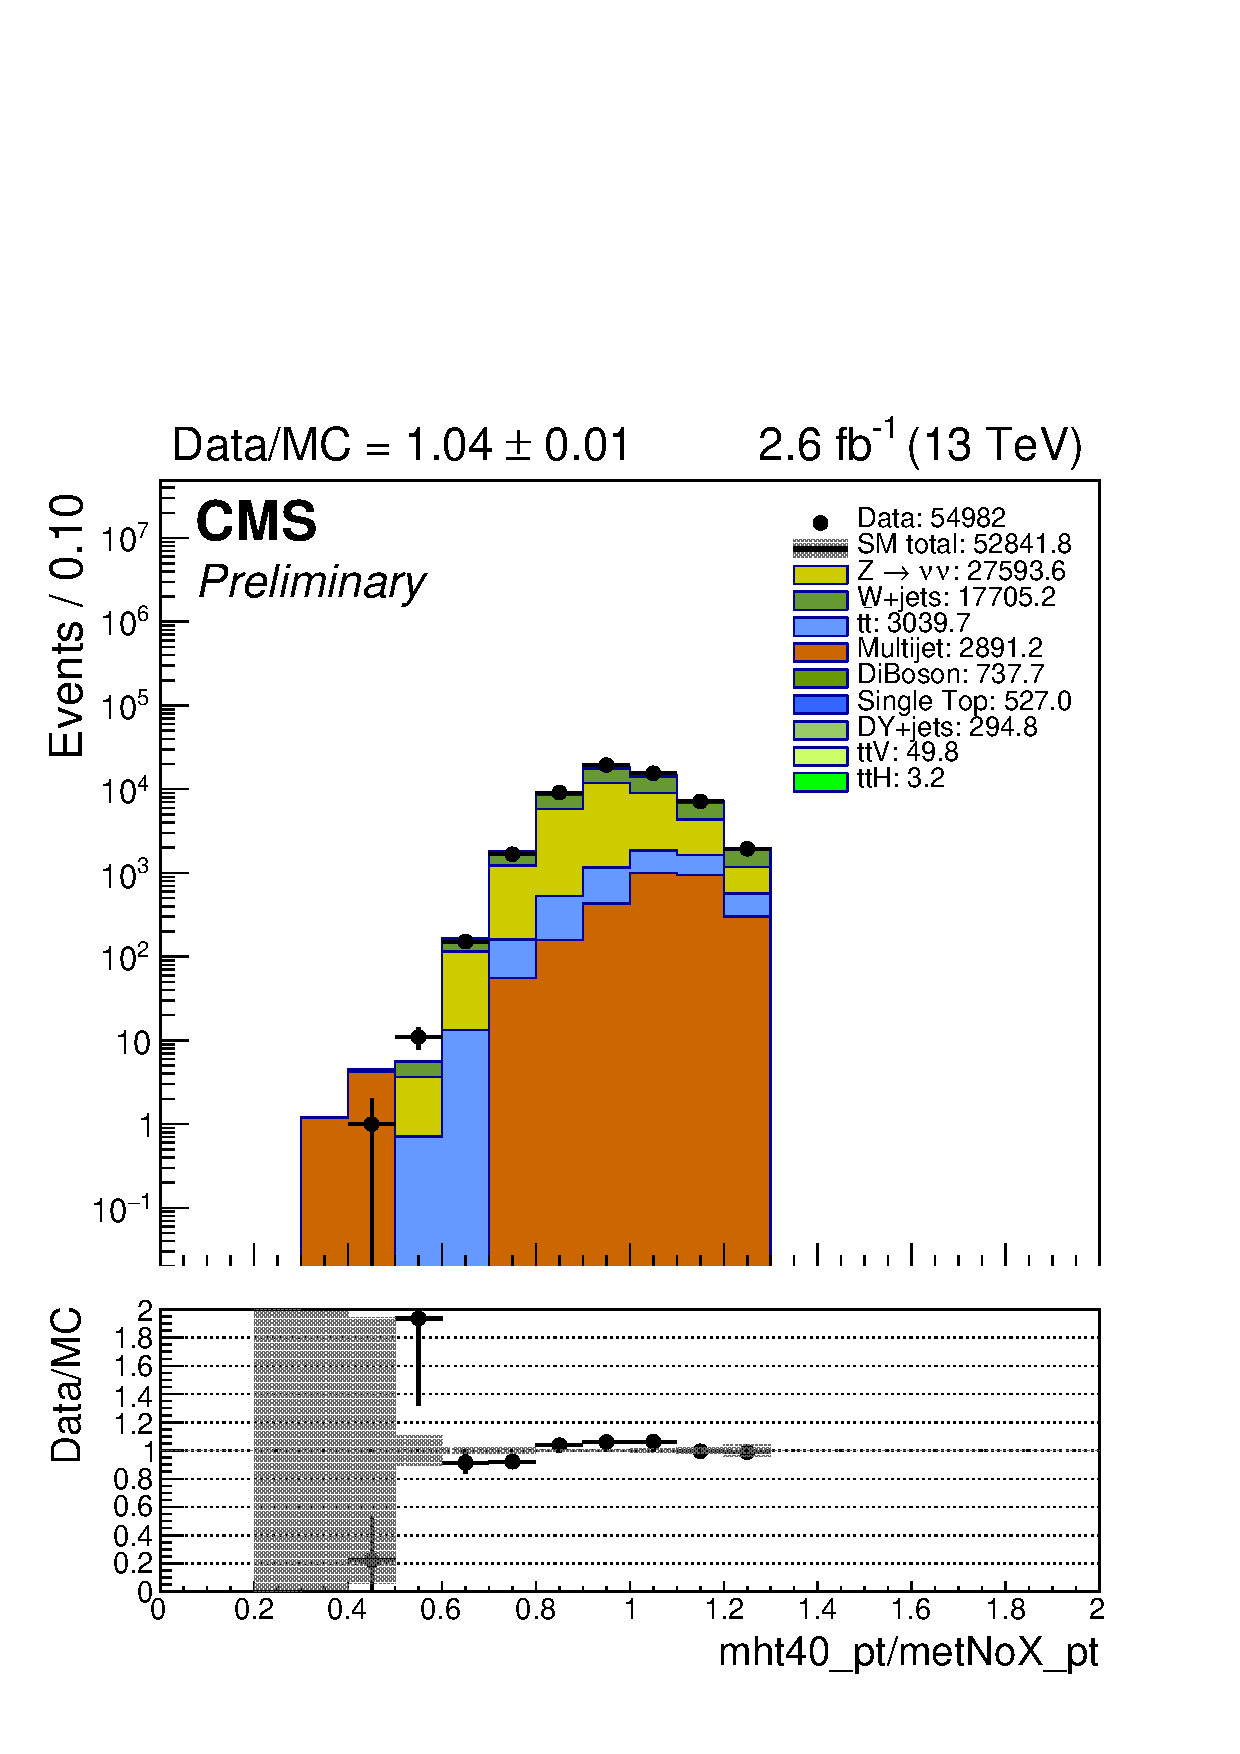
\includegraphics[width=0.5\textwidth]{figures/qcd/mhtDivMet/sr74X}
  % }~~ 
  \subfigure[\mhtmet distributions with 74X QCD
  MC that is scaled by 0.5]{
    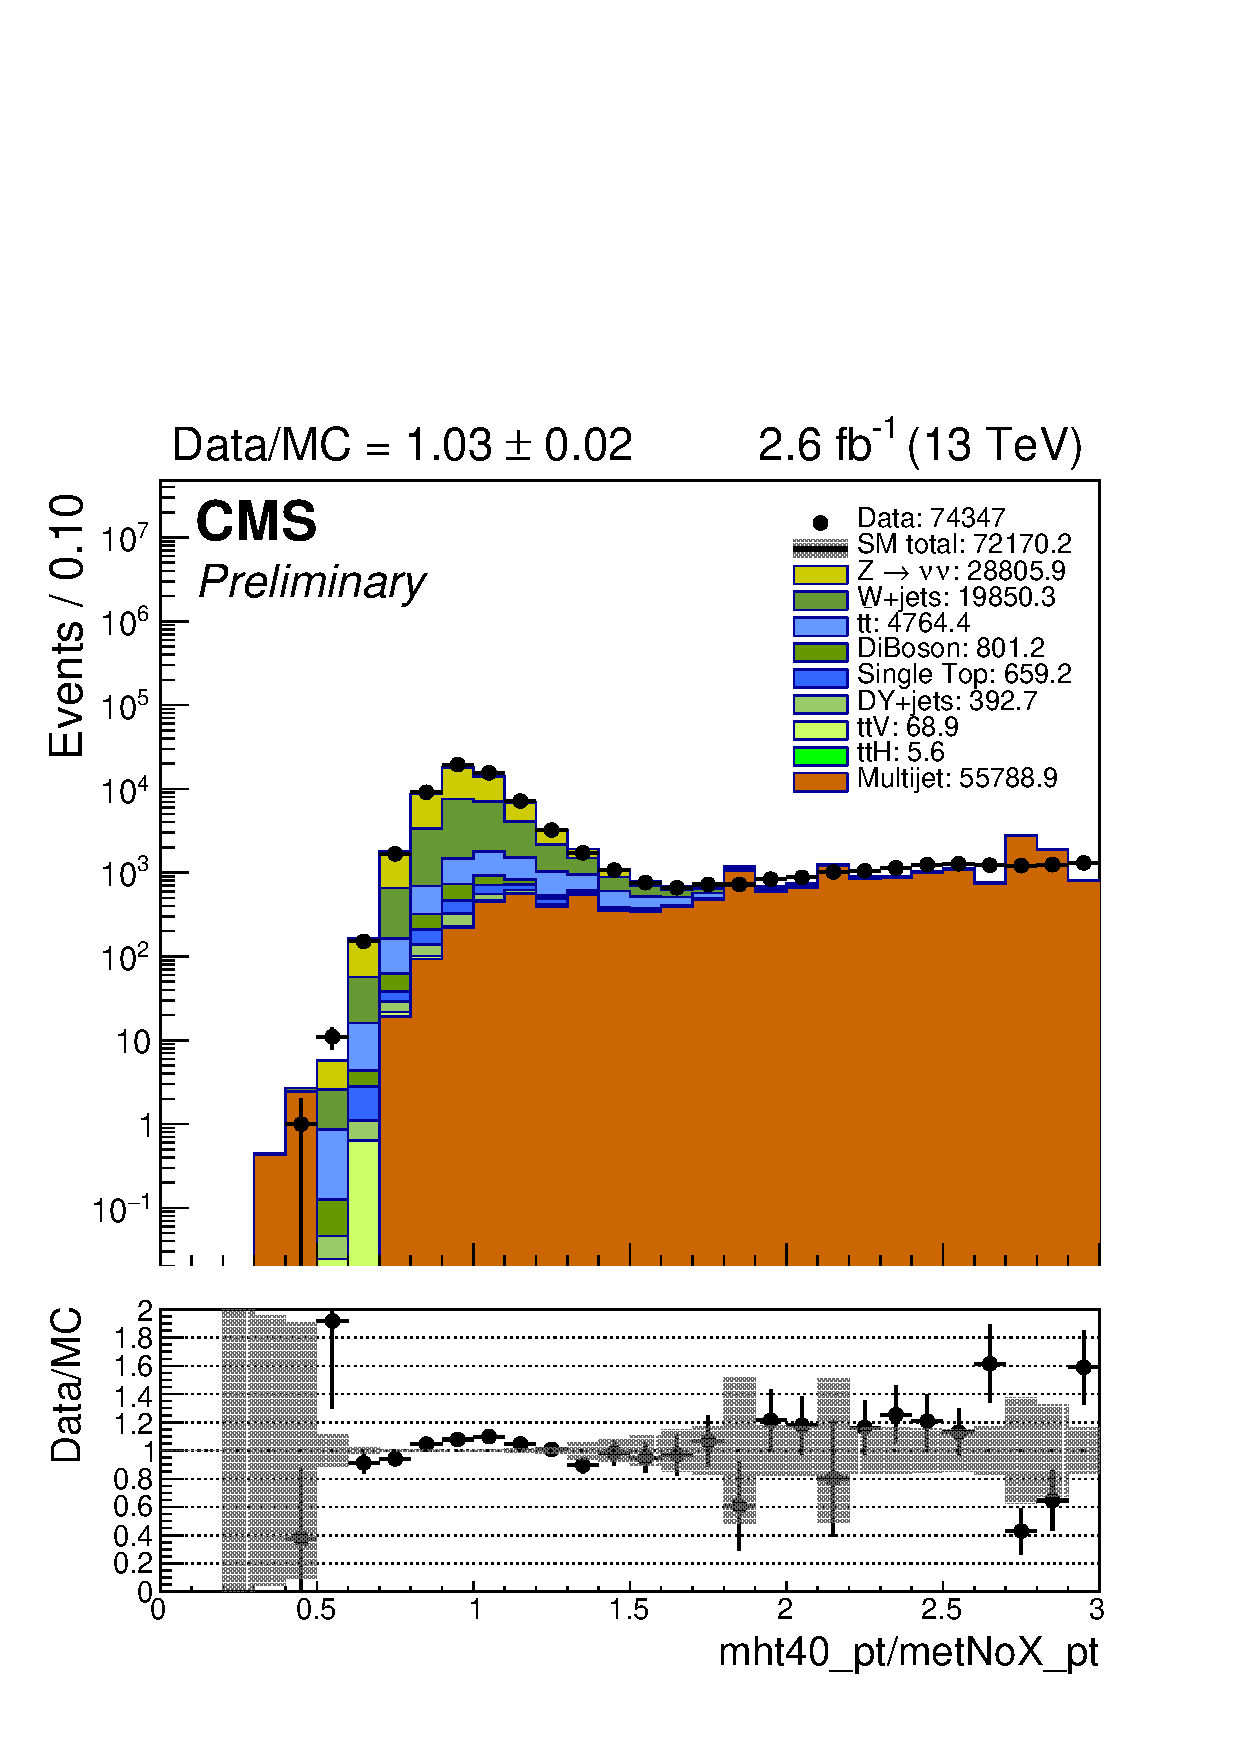
\includegraphics[width=0.5\textwidth]{figures/qcd/mhtDivMet/mht40_pt_Div_metNoX_pt_all_all_74X_noOverflow_scaled0p5}
  } ~~ 
  % \subfigure[\mhtmet distributions in the signal region with 80X QCD
  % MC.]{
  %   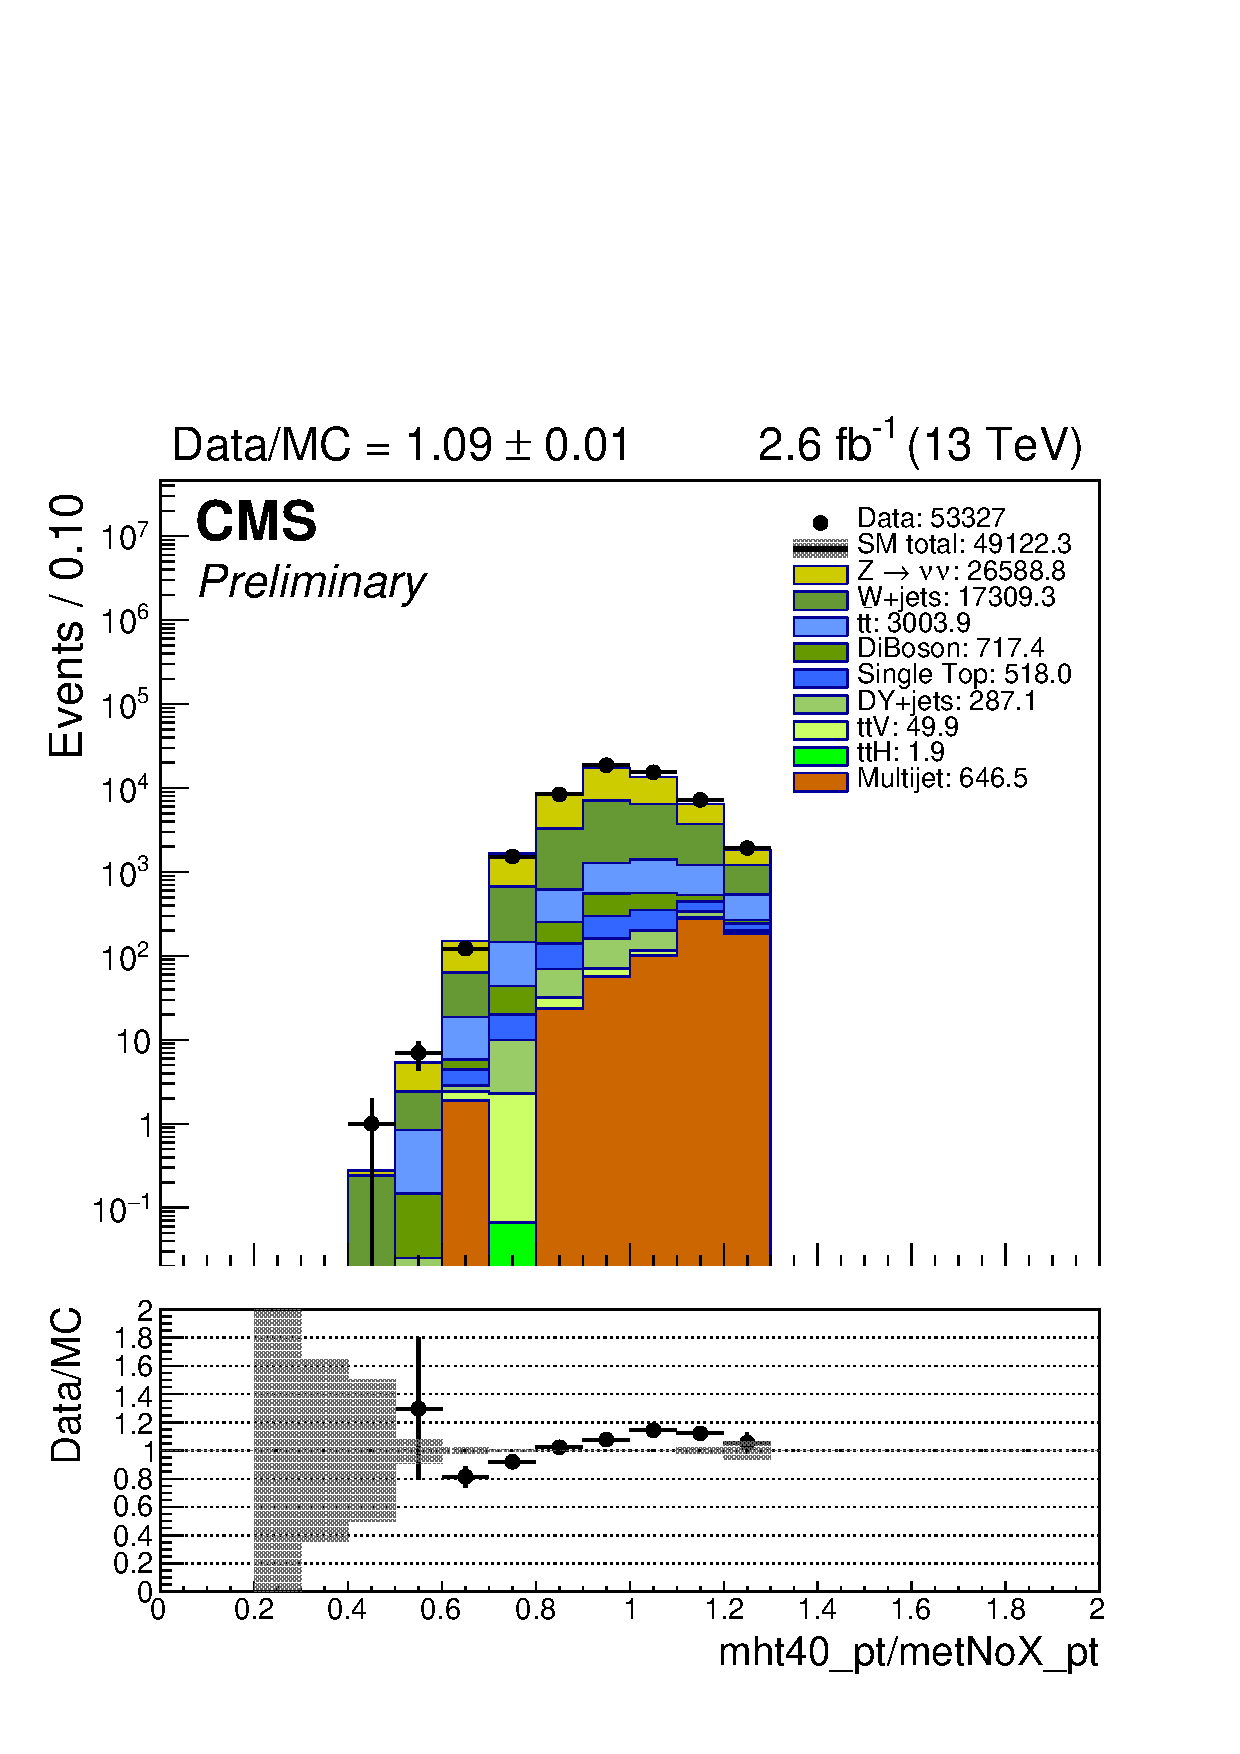
\includegraphics[width=0.5\textwidth]{figures/qcd/mhtDivMet/sr80X}
  % }~~
  \subfigure[\mhtmet distributions with 80X QCD
  MC that is scaled by 0.6]{
    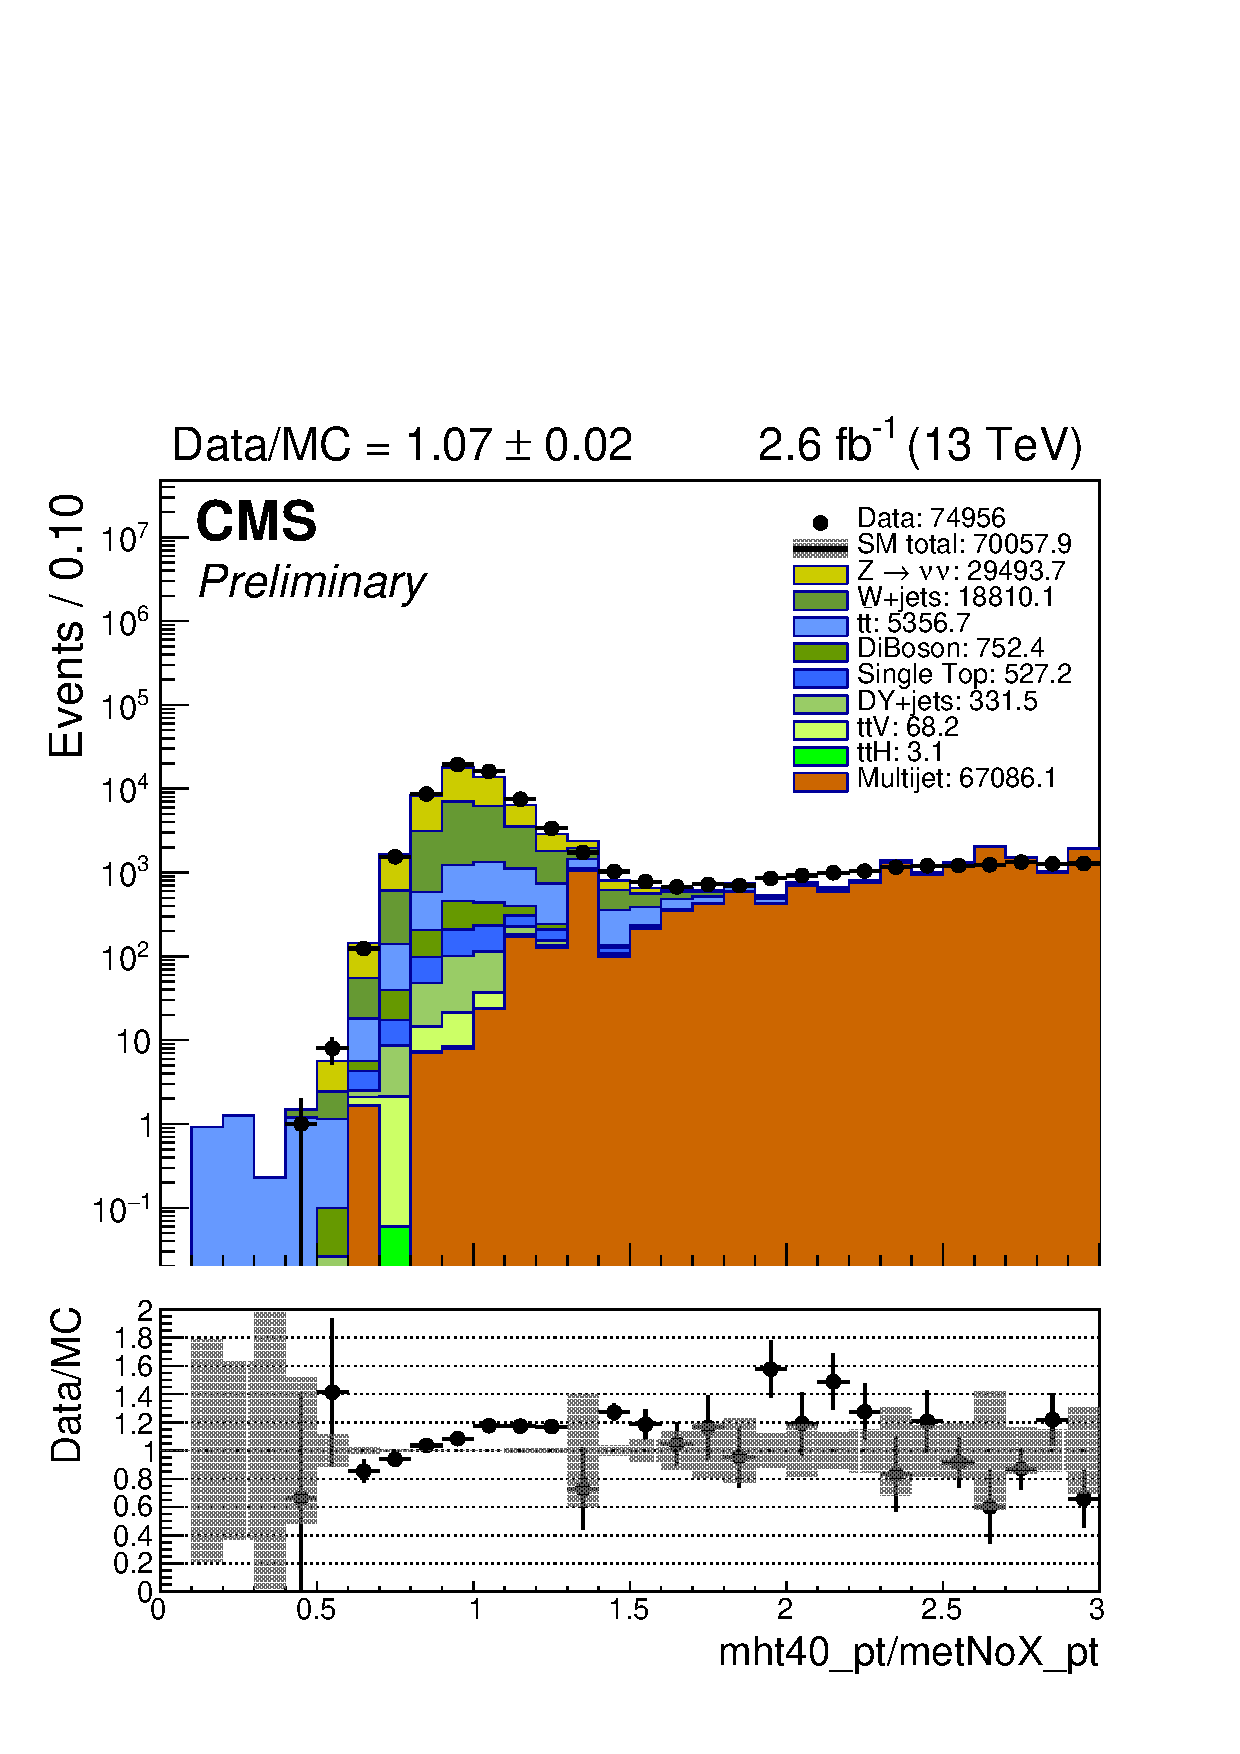
\includegraphics[width=0.5\textwidth]{figures/qcd/mhtDivMet/mht40_pt_Div_metNoX_pt_all_all_80X_noOverflow_scaled0p6}
  } \\
  \caption{The \mhtmet distributions for different versions of the QCD
  simulation. There is a significant change in the distribution
  between the MC reconstructed with CMSSW 74X and 80X. The QCD MC in
  each plot is rescaled to take account of normalisation mismodelling.}
  \label{fig:mhtDivMetChange}
\end{figure}


\subsection{Validation of the QCD prediction}
\label{sec:qcdValidation}

Despite being as data driven as possible, the method for predicting the QCD contamination in the signal region
described in Sec.~\ref{sec:qcdMethod} relies on the ratio, \rmhtmet,
of QCD counts
that is derived with simulation. This ratio is validated with data in a
QCD enriched sideband, where full signal region selection is used
other than
an inversion of the \bdphi cut to $\bdphi<0.5$. In this sideband a
data driven estimation of the QCD counts is carried out in two regions, those with \mhtmet values less than
1.25 and those with values greater than 1.25. These predictions are
made with a maximum likelihood
fit, analagous to that described in Sec.~\ref{sec:qcdMethod}. This fit
estimates the EWK counts with single muon, double muon and single
photon control regions and all relevant systematic errors. The
remaining data counts are then attributed to QCD. With this estimation 
of QCD it is possible to derive a data driven ratio of QCD counts with 
$\mhtmet<1.25$ and those with $\mhtmet>1.25$, $\rmhtmet_{\bdphi<0.5}^{data}$. By
taking MC counts in the \bdphi sideband it is also possible to
calculate the \mhtmet simulation ratio, $\rmhtmet_{\bdphi<0.5}$. 

To
validate the ratio \rmhtmet it is assumed that if the simulation of
the ratio in the \bdphi sideband agrees with that
derived from data, the simulated ratio that is not in the sideband
is valid. Any disagreement is covered by 
a systematic error on the signal region QCD prediction. The double ratio of
$\rmhtmet_{\bdphi<0.5}$ and $\rmhtmet_{\bdphi<0.5}^{data}$ in \scalht
and \njet bins is shown in Fig.~\ref{fig:RR_qcd}. Bins in which there
are insufficient statistics in data or simulation to make the calculation are left out.
This
plot illustrates that a fully correlated systematic of 100\% taken on the
predicted QCD contamination in the signal region should cover any
disagreement between simulation and data.

\begin{figure}[h!]
  \begin{center}        
    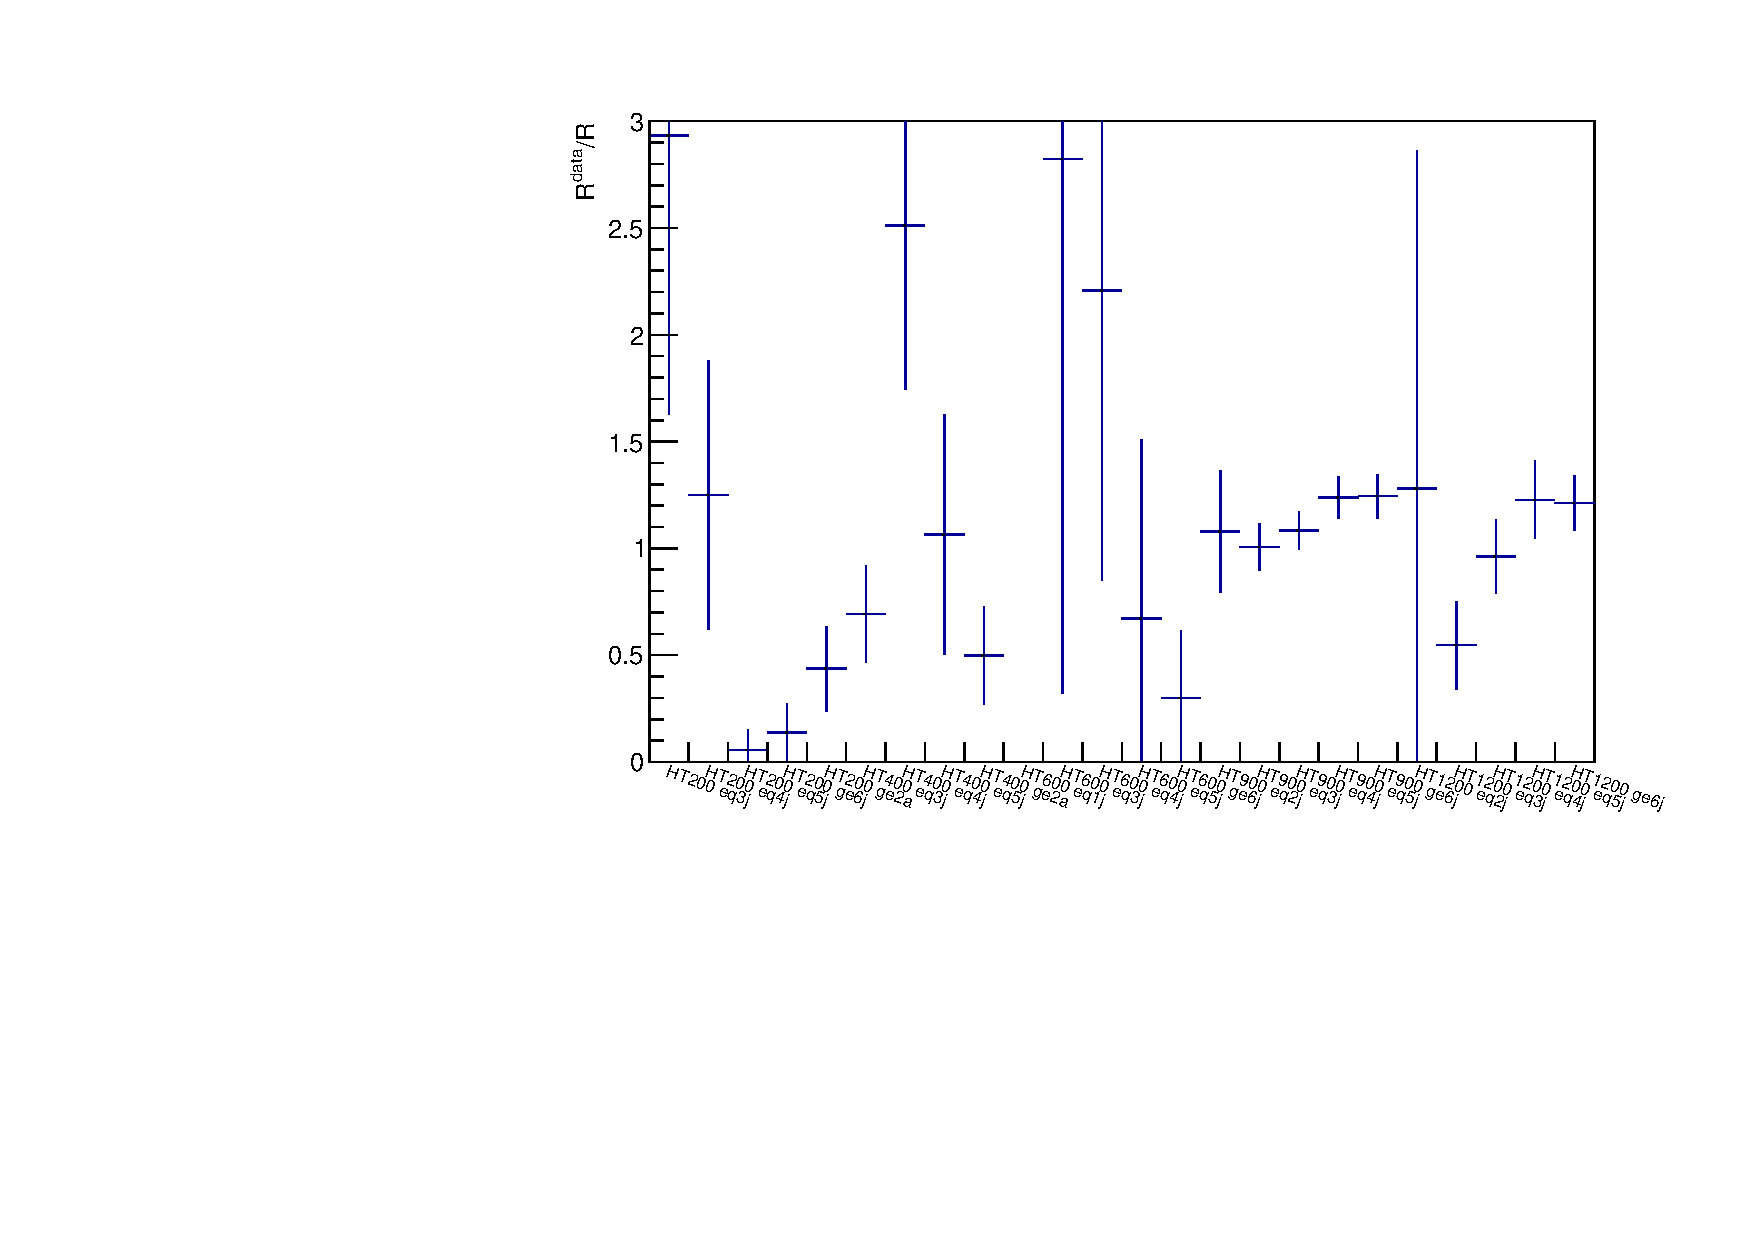
\includegraphics[width=\textwidth]{figures/qcd/plots/doubleQcdSbSrRatio1D}
    \caption{ Ratio of the measurement of \rmhtmet, the pass/fail ratio for the \mhtmet selection, from data and Monte Carlo in the $\bdphi < 0.5$ sideband in (\scalht, \njet) bins.  
    }

    \label{fig:RR_qcd}
  \end{center} 
\end{figure}

As the prediction of QCD in the signal region is carried out
inclusively over \nb and \mht, the QCD shapes for these variables are
taken from the EWK simulation and normalised to the QCD counts. 
A lack of statistics in
the QCD MC led to the adoption of this approach. To validate it, the simulated \mht distributions
for the QCD and EWK processes in the signal region are divided. This is shown in
Figs.~\ref{fig:asym_qcd_validation}-\ref{fig:asym_qcd_validation}.
As the normalisation is carried out independently, a flat distribution
of the ratio is enough for validation. Within uncertainties, the level of agreement is acceptable given the
small total QCD contribution to the signal region and its large
systematic uncertainty. 

\begin{figure}[h!]
  \begin{center}
    \subfigure[{ Asymmetric,
    $\scalht<400$~GeV}]{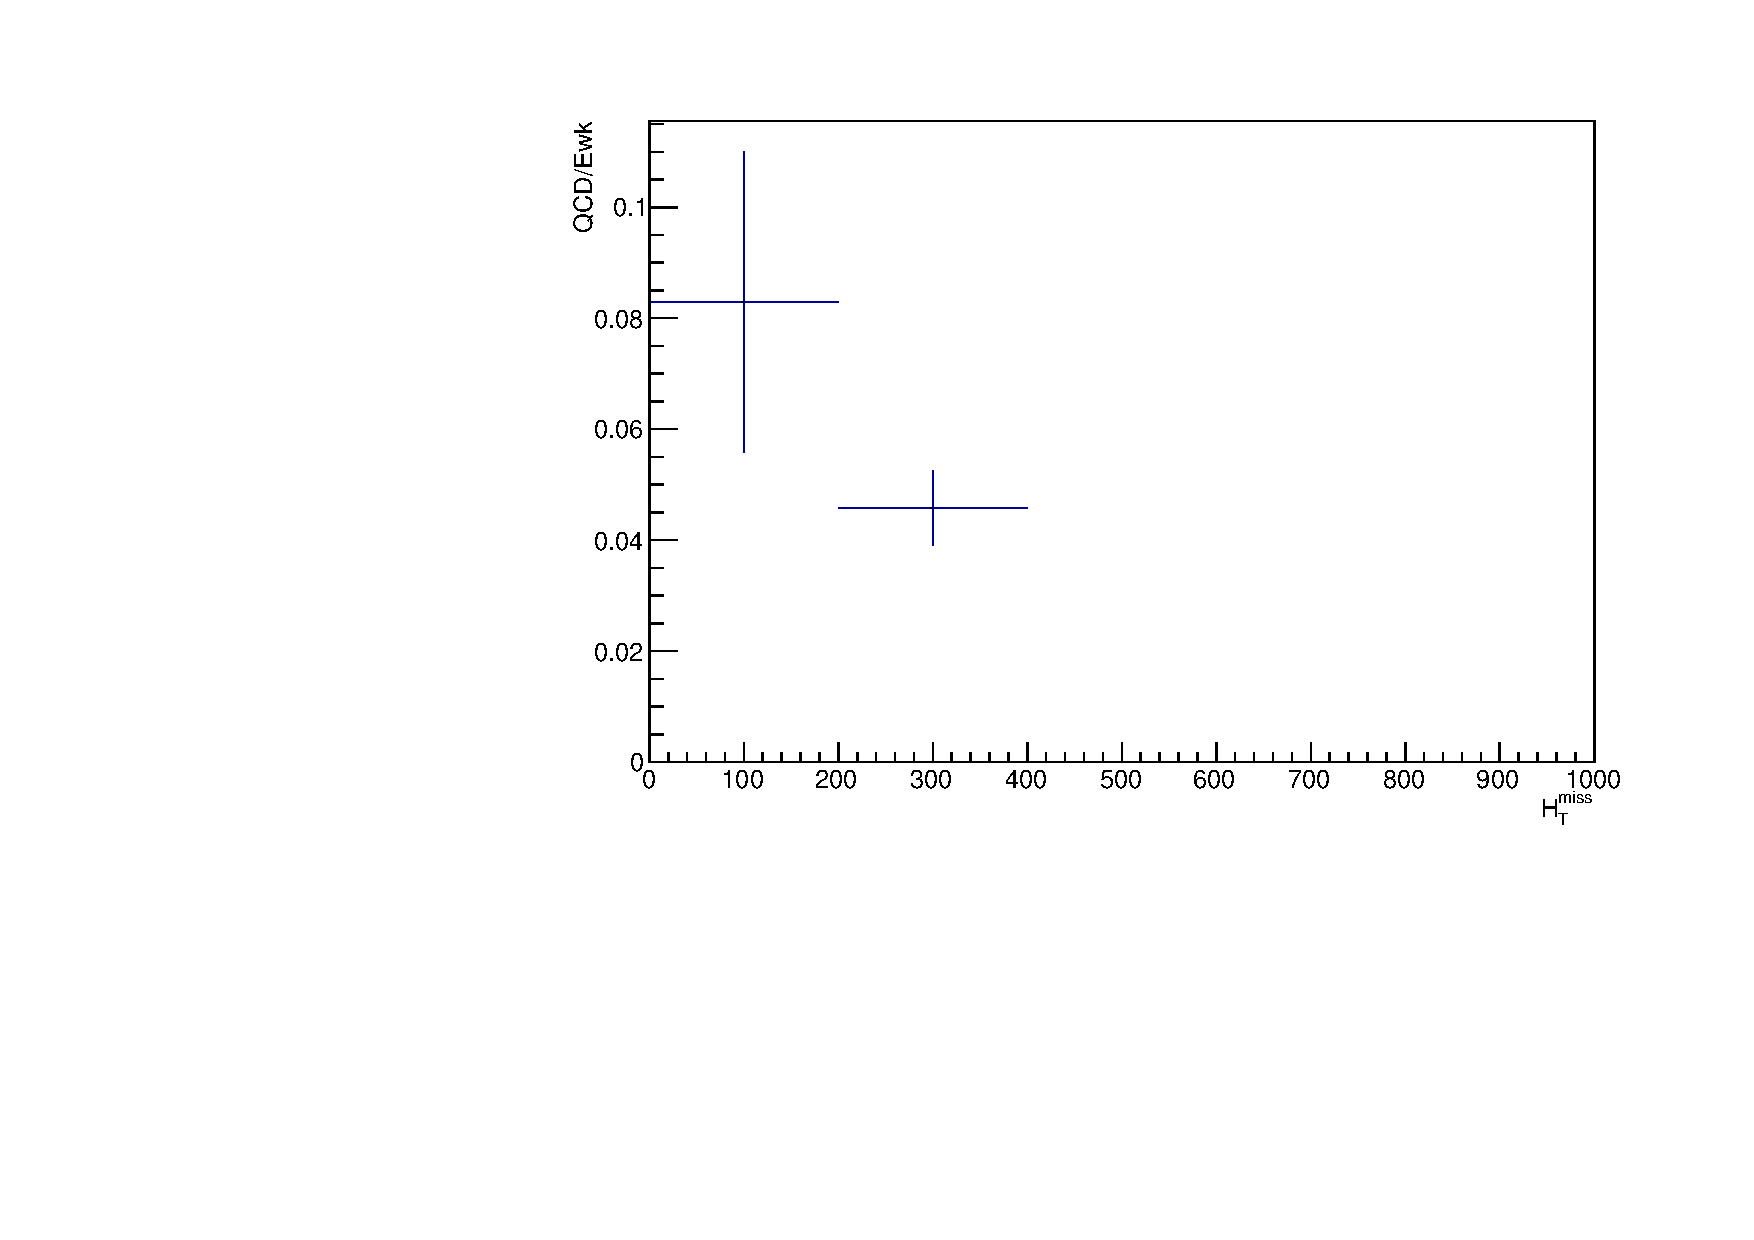
\includegraphics[width=0.5\textwidth]{figures/qcd/plots/mht_ht_lt400asym}} ~~
    \subfigure[{ Asymmetric,
    $\scalht<400$~GeV}]{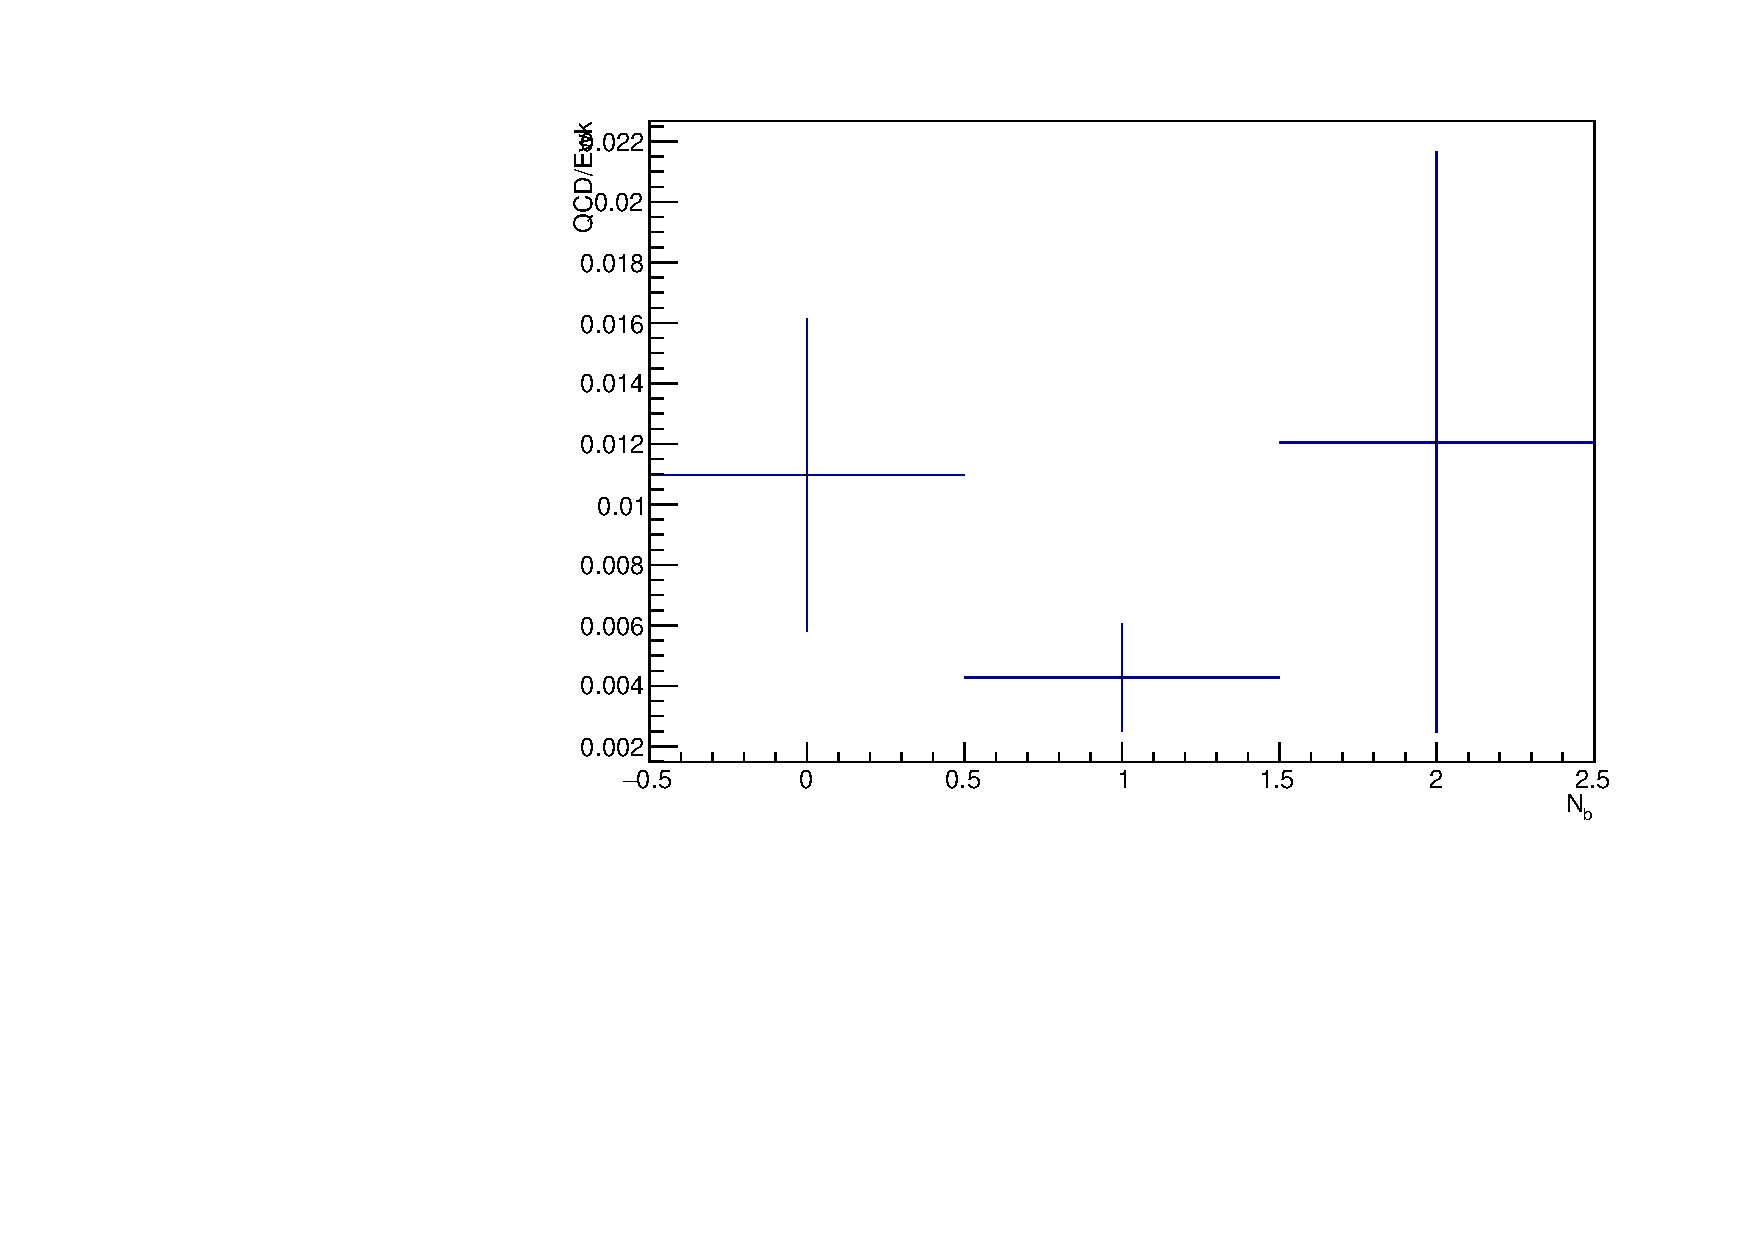
\includegraphics[width=0.5\textwidth]{figures/qcd/plots/nB_ht_lt400asym}} \\
    \subfigure[{ Asymmetric,
    $400<\scalht<800$~GeV}]{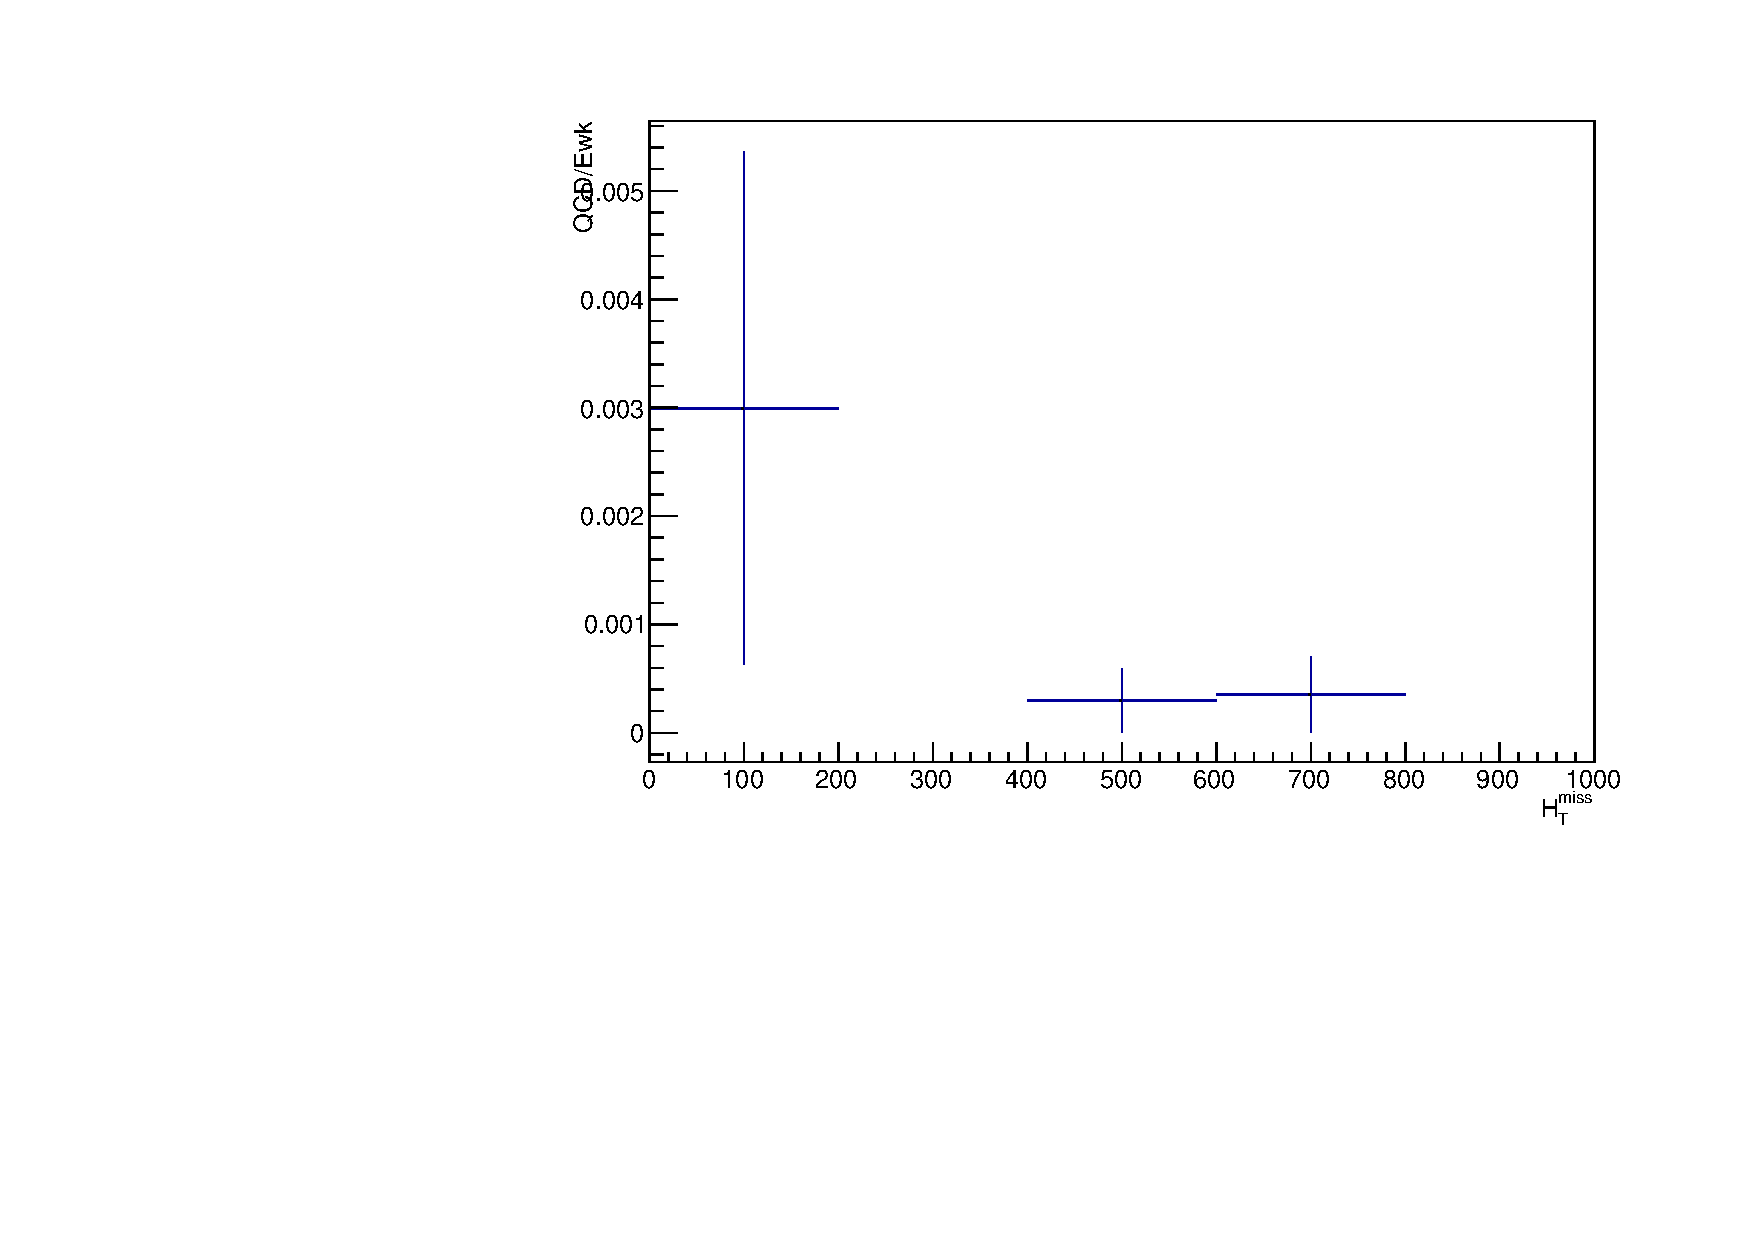
\includegraphics[width=0.5\textwidth]{figures/qcd/plots/mht_ht_lt800asym}} ~~
    \subfigure[{ Asymmetric,
    $400<\scalht<800$~GeV}]{\includegraphics[width=0.5\textwidth]{figures/qcd/plots/nB_ht_lt800asym}} \\
    \caption{ Ratio of QCD to electroweak Monte Carlo prediction in
    the signal region for different \scalht selections as a function
    of \mht (Left) and $\nb$ (Right) for the asymmetric jet category.
    %A constant fit to the data is represented by the red line, with the $\pm$100\% uncertainty represented by the blue hashed region.
    }
    \label{fig:asym_qcd_validation}
  \end{center} 
\end{figure}


\clearpage
\begin{figure}[h!]
  \begin{center}
    \subfigure[{ Symmetric,
    $\scalht<400$~GeV}]{\includegraphics[width=0.5\textwidth]{figures/qcd/plots/mht_ht_lt400sym}} ~~
    \subfigure[{ Symmetric,
    $\scalht<400$~GeV}]{\includegraphics[width=0.5\textwidth]{figures/qcd/plots/nB_ht_lt400sym}} \\
    \subfigure[{ Symmetric,
    $400<\scalht>800$~GeV}]{\includegraphics[width=0.5\textwidth]{figures/qcd/plots/mht_ht_lt800sym}} ~~
    \subfigure[{ Symmetric,
    $400<\scalht<800$~GeV}]{\includegraphics[width=0.5\textwidth]{figures/qcd/plots/nB_ht_lt800sym}} \\
    \subfigure[{ Symmetric,
    $\scalht>800$~GeV}]{\includegraphics[width=0.5\textwidth]{figures/qcd/plots/mht_ht_ltInfsym}} ~~
    \subfigure[{ Symmetric,
    $\scalht>800$~GeV}]{\includegraphics[width=0.5\textwidth]{figures/qcd/plots/nB_ht_ltInfsym}} \\
      \caption{ Ratio of QCD to electroweak Monte Carlo prediction in
      the signal region for different \scalht selections as a function
      of \mht (Left) and $\nb$ (Right) for the asymmetric jet
      category. %A constant fit to the data is represented by the red line, with the $\pm$100\% uncertainty represented by the blue hashed region.
    }
    \label{fig:sym_qcd_validation}
  \end{center} 
\end{figure}

%%____________________________________________________________________________||

\section{Background estimation for processes with genuine \met}

The dominant backgrounds with real \met is $Z$+jets production with the $Z$ boson decaying to neutrinos.
Smaller contributions come from $Z\to \ell \ell$ decays with both leptons
mis-reconstructed. The next largest background contribution is \wtaunu production. All of these background processes are dominated
by light jet and low to intermediate jet multiplicities. For $b$-jets jets and larger jet 
multiplicities contributions from single-top-quark, $\ttbar$V or $\ttbar$H and diboson production become relevant. We will refer
to these backgrounds as non-multijet or electroweak background.

The background simulations are normalised using the best known cross
section calculations currently available, usually with next-to-next-to-leading-order (NNLO) accuracy. 

\subsection{Transfer Factors}
\label{sec:ewk-method}

We use the transfer factor (TF) method to derive corrections to the background normalisations by testing their normalisations
in control regions. These control regions are identical in their energy scale \scalht, jet multiplicity \njet and $b$-jet multiplicity \nb 
as the signal region to be predicted. 

Each transfer factor is simply a ratio of the yields obtained from MC
simulation for the same bin of the signal region and a given control
sample:

\begin{equation}
  \label{equ:tf-ratio}
  {\rm TF} = \frac{N_{\rm MC}^{\rm signal}(\njet,\nb,\scalht)}{N_{\rm
      MC}^{\rm control}(\njet,\nb,\scalht)} 
\end{equation}

In this way, predictions of background counts from SM processes can be
made based on the various control samples:

\begin{equation}
  \label{equ:pred-method}
  \npre^{\rm signal}(\njet,\nb,\scalht) = \frac{N_{\rm MC}^{\rm
      signal}(\njet,\nb,\scalht)}{N_{\rm MC}^{\rm
      control}(\njet,\nb,\scalht)} \times \nobs^{\rm
    control}(\njet,\nb,\scalht)   
\end{equation}


Here \nobs corresponds to the background yield measure in a control region bin in $(\njet,\nb,\scalht)$ used to predict the 
ield \npre in the corresponding hadronic signal region bin $(\njet,\nb,\scalht)$.

%The selection criteria for the data control samples closely resemble
%those for the signal region, differing mainly through the use of a
%lepton or photon object {\it tag} (that is ignored in the calculation
%of jet-based kinematic variables such as \scalht, \mht, \alphat, \etc)
%and minimal additional kinematic requirements (\eg invariant or
%transerve mass windows) to obtain W, Z, and \ttbar-enriched event
%samples. The same selection criteria are designed to suppress signal
%contamination in the control samples so that unbiased data-driven
%estimates for the SM backgrounds in the signal region can be
%made. 


The transfer factors are designed to account for differences in cross sections times branching ratio, acceptance and reconstruction efficiencies and 
kinematic requirements between control and signal regions. As discussed in Sec.~\ref{selection} the control regions closely resemble the kinematics of the signal selections with the exception mandated to enrich the desired processes. While by using transfer factors one can cancels many systematic effects one still has to assign systematic uncertainties due to mis-modelling of kinematics  (\eg acceptances) and instrumental effects (\eg reconstruction efficiencies.)


The transfer factors from all four control regions are tabularized in Sec. 11 of \cite{alphaTnote}.
We give here as example the results for the \gj to \znunu transfer factors because they can be compared to similar methods in related WIMP searches.
These are shown in Tables~\ref{tab:tf_mu_zinv_asym}, \ref{tab:tf_mumu_zinv_sym}. 

\begin{table}[h!]
\tiny
\centering
\caption{Transfer factors from the \gj control region to the \zInv~ background for symmetric categories.\label{tab:tf_gj_zinv_sym}}
\scalebox{0.85}{\begin{tabular}{ccccc}
	\hline\hline
	& \multicolumn{4}{c}{\scalht (\gev)} \\ 
	 (\njet,  \nb) & 400-500 & 500-600 & 600-800 & 800-$\infty$ \\ [0.8ex] 
\hline
	(2, 0) & $0.78\pm 0.04$ & $0.72\pm 0.06$ & $0.54\pm 0.04$ & $0.28\pm 0.01$ \\[0.5ex] 
	(2, 1) & $0.82\pm 0.16$ & $0.71\pm 0.20$ & $0.78\pm 0.18$ & $0.24\pm 0.03$ \\[0.5ex] 
	(2, 2) & $0.64\pm 0.42$ & $1.93\pm 1.63$ & $0.52\pm 0.55$ & -- \\[0.5ex] 
	(3, 0) & $0.72\pm 0.04$ & $0.64\pm 0.04$ & $0.67\pm 0.03$ & $0.26\pm 0.01$ \\[0.5ex] 
	(3, 1) & $0.78\pm 0.10$ & $0.68\pm 0.11$ & $1.02\pm 0.17$ & $0.26\pm 0.03$ \\[0.5ex] 
	(3, 2) & $0.71\pm 0.28$ & $0.89\pm 0.55$ & $0.63\pm 0.28$ & $0.21\pm 0.07$ \\[0.5ex] 
	(3, $\ge3$) & -- & -- & -- & -- \\[0.5ex] 
	(4, 0) & $0.83\pm 0.05$ & $0.73\pm 0.05$ & $0.58\pm 0.03$ & $0.27\pm 0.01$ \\[0.5ex] 
	(4, 1) & $0.72\pm 0.11$ & $0.85\pm 0.15$ & $0.69\pm 0.09$ & $0.29\pm 0.03$ \\[0.5ex] 
	(4, 2) & $0.75\pm 0.25$ & $0.70\pm 0.30$ & $0.31\pm 0.10$ & $0.27\pm 0.06$ \\[0.5ex] 
	(4, $\ge3$) & $577.40\pm 664.02$ & $0.38\pm 0.44$ & $0.26\pm 0.31$ & $0.04\pm 0.05$ \\[0.5ex] 
	($\ge5$, 0) & $0.89\pm 0.13$ & $0.71\pm 0.08$ & $0.57\pm 0.04$ & $0.30\pm 0.01$ \\[0.5ex] 
	($\ge5$, 1) & $0.79\pm 0.22$ & $0.57\pm 0.12$ & $0.48\pm 0.07$ & $0.26\pm 0.02$ \\[0.5ex] 
	($\ge5$, 2) & $0.85\pm 0.54$ & $0.40\pm 0.16$ & $0.43\pm 0.15$ & $0.22\pm 0.04$ \\[0.5ex] 
	($\ge5$, $\ge3$) & -- & -- & $1.40\pm 1.47$ & $0.52\pm 0.33$ \\[0.5ex] 
	\hline
	\hline
\end{tabular}}
\end{table}

\begin{table}[h!]
\tiny
\centering
\caption{Transfer factors from the \gj control region to the \zInv~ background for asymmetric categories.\label{tab:tf_gj_zinv_asym}}
\begin{tabular}
{ccccc}
	\hline\hline
	& \multicolumn{4}{c}{\scalht (\gev)} \\ 
	 (\njet,  \nb) & 400-500 & 500-600 & 600-800 & 800-$\infty$ \\ [0.8ex] 
\hline
	(2a, 0) & $0.65^{+ 0.05 }_{- 0.05 }$ & $0.56^{+ 0.08 }_{- 0.08 }$ & $0.54^{+ 0.07 }_{- 0.07 }$ & -- \\[0.5ex] 
	(2a, 1) & $1.04^{+ 0.35 }_{- 0.35 }$ & $0.54^{+ 0.24 }_{- 0.24 }$ & -- & -- \\[0.5ex] 
	(2a, 2) & -- & -- & -- & -- \\[0.5ex] 
	(3a, 0) & $0.71^{+ 0.08 }_{- 0.08 }$ & $0.61^{+ 0.12 }_{- 0.12 }$ & $0.76^{+ 0.17 }_{- 0.17 }$ & -- \\[0.5ex] 
	(3a, 1) & $0.68^{+ 0.22 }_{- 0.22 }$ & $0.26^{+ 0.13 }_{- 0.13 }$ & $0.67^{+ 0.45 }_{- 0.45 }$ & -- \\[0.5ex] 
	(3a, 2) & $0.68^{+ 0.43 }_{- 0.43 }$ & $1.08^{+ 1.22 }_{- 1.22 }$ & -- & -- \\[0.5ex] 
	(3a, $\ge3$) & -- & -- & -- & -- \\[0.5ex] 
	(4a, 0) & $0.75^{+ 0.08 }_{- 0.08 }$ & $0.69^{+ 0.15 }_{- 0.15 }$ & $0.42^{+ 0.13 }_{- 0.13 }$ & -- \\[0.5ex] 
	(4a, 1) & $0.87^{+ 0.21 }_{- 0.21 }$ & $0.36^{+ 0.18 }_{- 0.18 }$ & $0.50^{+ 0.36 }_{- 0.36 }$ & -- \\[0.5ex] 
	(4a, 2) & $0.95^{+ 0.63 }_{- 0.63 }$ & -- & -- & -- \\[0.5ex] 
	(4a, $\ge3$) & -- & -- & -- & -- \\[0.5ex] 
	($\ge5$a, 0) & $0.66^{+ 0.09 }_{- 0.09 }$ & $0.69^{+ 0.18 }_{- 0.18 }$ & $0.83^{+ 0.27 }_{- 0.27 }$ & -- \\[0.5ex] 
	($\ge5$a, 1) & $0.84^{+ 0.34 }_{- 0.34 }$ & $0.57^{+ 0.28 }_{- 0.28 }$ & $1.90^{+ 1.88 }_{- 1.88 }$ & -- \\[0.5ex] 
	($\ge5$a, 2) & $0.72^{+ 0.55 }_{- 0.55 }$ & $276.67^{+ 282.97 }_{- 282.97 }$ & -- & -- \\[0.5ex] 
	($\ge5$a, $\ge3$) & -- & -- & -- & -- \\[0.5ex] 
	\hline
	\hline
\end{tabular}
\end{table}



The uncertainty shown is from MC statistics only, the systematic uncertainty on the TFs is discussed in Sec.~\ref{sec:systematics}.
The scale factor decreases for larger \HT and behaves consistently across all jet multiplicities and \HT bins. 
The choice of a TF for each signal region bin is conservative as the prediction is made from control regions with similar kinematics
to the signal region bin (without extrapolation) which leads to larger statistical uncertainties.

The transfer factors define the overall background normalisation in each signal region bin (\njet,\nb,\HT) bin. These bins are
integrated over \mht. In each bin the shape of the \mht distribution is taken from simulations and then propagated to the likelihood model. 
A separate \mht template is used per (\njet,\nb,\HT) bin.



%%____________________________________________________________________________||
\section{Systematic uncertainties in the transfer factors}
\label{sec:systematics}

This section addresses the estimation of systematic uncertainties
affecting the transfer factors (equation~\ref{equ:tf-ratio})
for non-multijet backgrounds. 
These uncertainties will be often referred to as \textit{``normalisation uncertainties''}, 
as opposed to the \textit{``template uncertainties''} described in Sec.~\ref{sec:syst-on-shape}. 
The former affect the total number of events in each (\njet,~\nb,~\scalht) bin (integrating over \mht), 
while the latter encode the limited knowledge on how these events distribute in the \mht dimension.

Two approaches are used to derive uncertainties from specific sources:
one is based on variations in simulation (Sec.~\ref{sec:mc-variations}), the other makes use of control samples in data (Sec.~\ref{sec:closure-tests}).
Each systematic source considered in the analysis is described below, 
together with the method used to derive the corresponding uncertainties and the correlation model. 
A summary of the all the uncertainties is given in Tab.~\ref{tab:systs}.



%% %%%%%%%%%%%%%%%%%%%%%%%%%%%%%%%%%%%%%%%%%%%%%%%%%%%%%%%%%%%%%%%%
%% % MC-based systematics
%% %%%%%%%%%%%%%%%%%%%%%%%%%%%%%%%%%%%%%%%%%%%%%%%%%%%%%%%%%%%%%%%%
\subsection{Systematic variations in simulation}
\label{sec:mc-variations}
A set of corrections are applied to the MC samples in order to improve the modelling 
of detector effects (b-tagging efficiency, jet energy response, etc.) 
as well as the simulation of the kinematics of certain processes (top $p_{T}$). 
These corrections are described in Sec.~\ref{sec:datasets}. \\
In this section the effect of varying these corrections within their uncertainties is 
presented, focusing on the relative change in the 4 type of transfer factors which are of interest 
for the background prediction, namely: $\mj \rightarrow (\znunu)$,
$\mmj \rightarrow (\znunu)$, $\gj \rightarrow (\znunu)$ and $\mj
\rightarrow \mathrm{\ttbar+W}$. 
The binning of the analysis is chosen in order to minimise the impact of 
these systematic sources, which are expected to be sub-dominant. 
However, they are propagated to the final results, taking into account correlations and bin migration effects.


\subsubsection*{Jet energy scale}
\label{sec:tfSyst_jec}
The effect of varying the jet energy scale in
the \mj and \mmj control regions is investigated.  The energies of
jets used in the analysis are corrected as a function of their \pt and
$\eta$ via the procedure recommended by the JetMET POG. These
corrections have an associated uncertainty, which is propagated through the analysis. 
As the \scalht and jet multiplicity binning is mirrored in signal and control regions, 
the effect of jet energy scale on the transfer factor is expected to be small. 
However, the jet energy scale can still have an
effect due to jets moving in and out acceptance (above and below
$40\gev$). The relative change in the transfer factors is presented as a function of \scalht and jet category 
in Fig. ~\ref{fig:tfSyst_jec_muToZinv}-\ref{fig:tfSyst_jec_muToTtw}.
The changes are typically in the range of $1-15\%$.


\begin{figure}[!h]
  \centering
  \subfigure[JEC up variation]{
    \includegraphics[width=0.5\textwidth]{figures/mcSystematics6p26Fb/Zinv/mu/ratiotfh_ht_mht_alljecWeight_Up.pdf}
  } ~~
  \subfigure[JEC down variation]{
    \includegraphics[width=0.5\textwidth]{figures/mcSystematics6p26Fb/Zinv/mu/ratiotfh_ht_mht_alljecWeight_Down.pdf}
  }\\

  \caption{\label{fig:tfSyst_jec_muToZinv} The relative change in the
  $\mj \rightarrow (\znunu)$ transfer
  factors when varying JEC in MC within its uncertainties, as a function of \scalht and jet category. 
  Variations corresponding to $+1\sigma$ ($-1\sigma$) are shown in the left (right) figure. 
  }
\end{figure}

\begin{figure}[!h]
  \centering
  \subfigure[JEC up variation]{
    \includegraphics[width=0.5\textwidth]{figures/mcSystematics6p26Fb/Zinv/mumu/ratiotfh_ht_mht_alljecWeight_Up.pdf}
  } ~~
  \subfigure[JEC down variation]{
    \includegraphics[width=0.5\textwidth]{figures/mcSystematics6p26Fb/Zinv/mumu/ratiotfh_ht_mht_alljecWeight_Down.pdf}
  }\\

  \caption{\label{fig:tfSyst_jec_mumuToZinv} The relative change in
  the $\mmj \rightarrow (\znunu)$ transfer
  factors when varying JEC in MC within its uncertainties, as a function of \scalht and jet category. 
  Variations corresponding to $+1\sigma$ ($-1\sigma$) are shown in the left (right) figure. 
  }
\end{figure}

\begin{figure}[!h]
  \centering
  \subfigure[JEC up variation]{
    \includegraphics[width=0.5\textwidth]{figures/mcSystematics6p26Fb/Zinv/gj/ratiotfh_ht_mht_alljecWeight_Up.pdf}
  } ~~
  \subfigure[JEC down variation]{
    \includegraphics[width=0.5\textwidth]{figures/mcSystematics6p26Fb/Zinv/gj/ratiotfh_ht_mht_alljecWeight_Down.pdf}
  }\\

  \caption{\label{fig:tfSyst_jec_gjToZinv} The relative change in the
  $\gj \rightarrow (\znunu)$ transfer
  factors when varying JEC in MC within its uncertainties, as a function of \scalht and jet category. 
  Variations corresponding to $+1\sigma$ ($-1\sigma$) are shown in the left (right) figure. 
  }
\end{figure}

\begin{figure}[!h]
  \centering
  \subfigure[JEC up variation]{
    \includegraphics[width=0.5\textwidth]{figures/mcSystematics6p26Fb/Ttw/mu/ratiotfh_ht_mht_alljecWeight_Up.pdf}
  } ~~
  \subfigure[JEC down variation]{
    \includegraphics[width=0.5\textwidth]{figures/mcSystematics6p26Fb/Ttw/mu/ratiotfh_ht_mht_alljecWeight_Down.pdf}
  }\\

  \caption{\label{fig:tfSyst_jec_muToTtw} The relative change in the
  $\mj \rightarrow \mathrm{\ttbar+W}$ transfer
  factors when varying JEC in MC within its uncertainties, as a function of \scalht and jet category. 
  Variations corresponding to $+1\sigma$ ($-1\sigma$) are shown in the left (right) figure. 
  }
\end{figure}




\subsubsection*{B-tagging efficiency}
\label{sec:tfSyst_btag}
Scale factors provided by the BTV POG are applied to the MC samples
to correct for differences in the b-tagging efficiencies and 
misidentifications between simulation and data. 
The method employed is
based on simple event reweighting as described in
Ref.~\cite{btagSFMethods}. As the scale factors for the data collected in
2016 are not yet available the systematics shown below are based 
on those from 2015. These uncertainties are not applied for the results in \ref{sec:results},
but will be rederived and included when the necessary scale factors are available.
Events are reweighted according to the probability of obtaining a particular jet configuration in data
and simulation, as determined by the b-tagging efficiencies computed
in the MC samples and the scale factors measured in data.
Since no extrapolation is performed in the background prediction across different 
\nb  multiplicities, the analysis is expected to be robust against variation in the 
b-tag efficiency. 
To test this effect the change in the transfer factors is measured
by varying the scale factors within their uncertainties. 
The relative change in the transfer factors is presented as a function of \scalht and jet category 
in Fig. ~\ref{fig:tfSyst_bsf_muToZinv}-\ref{fig:tfSyst_bsf_muToTtw}.
They are typically in the range of $1-5\%$.


\begin{figure}[!h]
  \centering
  \subfigure[b-tag SF up variation]{
    \includegraphics[width=0.5\textwidth]{figures/mcSystematics6p26Fb/Zinv/mu/ratiotfh_ht_mht_allbsfWeight_Up.pdf}
  } ~~
  \subfigure[b-tag SF down variation]{
    \includegraphics[width=0.5\textwidth]{figures/mcSystematics6p26Fb/Zinv/mu/ratiotfh_ht_mht_allbsfWeight_Down.pdf}
  }\\

  \caption{\label{fig:tfSyst_bsf_muToZinv} The relative change in the
  $\mj \rightarrow (\znunu)$ transfer
  factors when varying b-tag SF in MC within its uncertainties, as a function of \scalht and jet category. 
  Variations corresponding to $+1\sigma$ ($-1\sigma$) are shown in the left (right) figure. 
  }
\end{figure}

\begin{figure}[!h]
  \centering
  \subfigure[b-tag SF up variation]{
    \includegraphics[width=0.5\textwidth]{figures/mcSystematics6p26Fb/Zinv/mumu/ratiotfh_ht_mht_allbsfWeight_Up.pdf}
  } ~~
  \subfigure[b-tag SF down variation]{
    \includegraphics[width=0.5\textwidth]{figures/mcSystematics6p26Fb/Zinv/mumu/ratiotfh_ht_mht_allbsfWeight_Down.pdf}
  }\\

  \caption{\label{fig:tfSyst_bsf_mumuToZinv} The relative change in
  the $\mmj \rightarrow (\znunu)$ transfer
  factors when varying b-tag SF in MC within its uncertainties, as a function of \scalht and jet category. 
  Variations corresponding to $+1\sigma$ ($-1\sigma$) are shown in the left (right) figure. 
  }
\end{figure}

\begin{figure}[!h]
  \centering
  \subfigure[b-tag SF up variation]{
    \includegraphics[width=0.5\textwidth]{figures/mcSystematics6p26Fb/Zinv/gj/ratiotfh_ht_mht_allbsfWeight_Up.pdf}
  } ~~
  \subfigure[b-tag SF down variation]{
    \includegraphics[width=0.5\textwidth]{figures/mcSystematics6p26Fb/Zinv/gj/ratiotfh_ht_mht_allbsfWeight_Down.pdf}
  }\\

  \caption{\label{fig:tfSyst_bsf_gjToZinv} The relative change in the
  $\gj \rightarrow (\znunu)$ transfer
  factors when varying b-tag SF in MC within its uncertainties, as a function of \scalht and jet category. 
  Variations corresponding to $+1\sigma$ ($-1\sigma$) are shown in the left (right) figure. 
  }
\end{figure}

\begin{figure}[!h]
  \centering
  \subfigure[b-tag SF up variation]{
    \includegraphics[width=0.5\textwidth]{figures/mcSystematics6p26Fb/Ttw/mu/ratiotfh_ht_mht_allbsfWeight_Up.pdf}
  } ~~
  \subfigure[b-tag SF down variation]{
    \includegraphics[width=0.5\textwidth]{figures/mcSystematics6p26Fb/Ttw/mu/ratiotfh_ht_mht_allbsfWeight_Down.pdf}
  }\\

  \caption{\label{fig:tfSyst_bsf_muToTtw} The relative change in the $\mj \rightarrow \mathrm{tt+W}$ transfer
  factors when varying b-tag SF in MC within its uncertainties, as a function of \scalht and jet category. 
  Variations corresponding to $+1\sigma$ ($-1\sigma$) are shown in the left (right) figure. 
  }
\end{figure}





\subsubsection*{Lepton and photon trigger/identification/isolation efficiency}
\label{sec:tfSyst_lepton}
Leptons out of $p_{T}$ and $\eta$ acceptance, or within detector
acceptance but not identified properly by lepton identification or isolation
requirements contribute to the so-called ``lost-lepton background'', 
which mainly stem from W and \ttbar events. 
The fraction of events with leptons out of acceptance ($f_{sample}$)
is calculated from generator truth level information for each MC
sample. Differences in efficiencies between data and simulation are
accounted for with data/MC scale
factors for trigger, lepton identification and isolation~\cite{twiki-leptonSF}. 
The uncertainties on the transfer factors associated 
with these scale factors are determined as described in the following.
To cover issues in the efficiency of the
muon trigger a $5\%$ systematic is assigned for both the \mj and \mmj 
control regions as described in \ref{sec:disclaimers}. To cover 
issues in the photon trigger (as described in \ref{sec:disclaimers}) a $5\%$ is applied in the
\gj control region.

The effect of lepton reconstruction in the $\mj \rightarrow \mathrm{tt+W}$ 
transfer factors is factorised in the following expression: 
\begin{equation}
    \label{eq:lostLepTF}
    y = \frac{\sum_{sample} [ R_{sample} \times f_{sample} \times N^{GEN}_{sample} \times ( 1 - \epsilon_{Loose} ) + ( 1 - f_{sample} ) \times N^{GEN}_{sample} ]}{ \sum_{sample} N^{GEN}_{sample} \times \epsilon_{Tight} \times R_{sample} }
\end{equation}
where $R_{sample}$ is the cross section reweighting factor for each sample, 
$N^{GEN}_{sample}$ is the total MC events for the category, $\epsilon_{Tight}$
and $\epsilon_{Loose}$ are the lepton efficiency for Tight and Loose working 
point. The variable $y$ is computed for each category. For the numerator, full
signal selection except the lepton veto to mimic signal region phase space as
closely as possible. For the denominator, the full selection for the \mj 
control sample is applied.

The variation on the variable $y$ is computed by varying the lepton scale factor
up and down according to each source of uncertainty.
Data/MC lepton scale factors have negligible statistical uncertainties. 
The procedure is repeated separately for muons and
electrons.
Systematic uncertainties of 2\% are assigned to the efficiency of the muon and electron veto working point efficiency and taken as correlated across all the signal region bins. 

%The relative change in the $\mj \rightarrow \mathrm{tt+W}$ transfer factors 
%is presented in Fig.~\ref{fig:lostLepton}. The
%total change is typically in the range $2-5\%$

%\begin{figure}[!h]
%  \centering
%  \subfigure[Lepton scale factors varied up (muons)]{
%    \includegraphics[width=0.5\textwidth]{figures/mcSystematics/lostLepton/muonUp.pdf}
%  } ~~
%  \subfigure[Lepton scale factors varied down (muons)]{
%    \includegraphics[width=0.5\textwidth]{figures/mcSystematics/lostLepton/muonDown.pdf}
%  }\\
%  \subfigure[Scale factors varied up (electrons)]{
%    \includegraphics[width=0.5\textwidth]{figures/mcSystematics/lostLepton/electronUp.pdf}
%  } ~~
%  \subfigure[Scale factors varied down (electrons)]{
%    \includegraphics[width=0.5\textwidth]{figures/mcSystematics/lostLepton/electronDown.pdf}
%  }\\
%  \caption{\label{fig:lostLepton} 
%    Relative uncertainties for the ``lost-lepton'' ($\mathrm{tt+W}$) background due to lepton efficiency. 
%    The total uncertainty on the muons (electrons) is shown in the top (bottom) row.
%  }
%  
%\end{figure}



\subsubsection*{Photon trigger uncertainty}
\label{sec:tfSyst_photonTrigger}

Variations in the trigger weight for the signal region are studied. A conservative systematic
uncertainty on this correction is taken as the size of the inefficiency. 
The relative change in the \gj transfer factor is presented in Fig.~\ref{fig:tfSyst_photonTrigger_gjToZinv}
variation is typically in the range $0-3\%$.


\begin{figure}[!h]
  \centering
  \subfigure[Photon trigger weight up variation]{
    \includegraphics[width=0.5\textwidth]{figures/mcSystematics6p26Fb/Zinv/gj/ratiotfh_ht_mht_allphotonTriggerWeight_Up.pdf}
  } ~~
  \subfigure[Photon trigger weight down variation]{
    \includegraphics[width=0.5\textwidth]{figures/mcSystematics6p26Fb/Zinv/gj/ratiotfh_ht_mht_allphotonTriggerWeight_Down.pdf}
  }\\

  \caption{\label{fig:tfSyst_photonTrigger_gjToZinv} The relative change in
  the $\gj \rightarrow (\znunu)$ transfer
  factors when varying photon trigger weight in MC within its uncertainties, as a function of \scalht and jet category. 
  Variations corresponding to $+1\sigma$ ($-1\sigma$) are shown in the left (right) figure. 
  }
\end{figure}

\subsubsection*{Signal trigger uncertainty}
\label{sec:tfSyst_trigger}

Variations in the trigger weight for the signal region are studied. A systematic is taken
as the difference in the efficiency measured using muon and electron reference triggers.
The relative change in transfer factors is presented in Fig.
~\ref{fig:tfSyst_trigger_muToZinv}-\ref{fig:tfSyst_trigger_muToTtw}. The
variation is typically in the range $0-5\%$.

\begin{figure}[!h]
  \centering
  \subfigure[trigger weight up variation]{
    \includegraphics[width=0.5\textwidth]{figures/mcSystematics6p26Fb/Zinv/mu/ratiotfh_ht_mht_alltriggerWeight_Up.pdf}
  } ~~
  \subfigure[trigger weight down variation]{
    \includegraphics[width=0.5\textwidth]{figures/mcSystematics6p26Fb/Zinv/mu/ratiotfh_ht_mht_alltriggerWeight_Down.pdf}
  }\\

  \caption{\label{fig:tfSyst_trigger_muToZinv} The relative change in
  the $\mj \rightarrow (\znunu)$ transfer
  factors when varying trigger weight in MC within its uncertainties, as a function of \scalht and jet category. 
  Variations corresponding to $+1\sigma$ ($-1\sigma$) are shown in the left (right) figure. 
  }
\end{figure}
\begin{figure}[!h]
  \centering
  \subfigure[trigger weight up variation]{
    \includegraphics[width=0.5\textwidth]{figures/mcSystematics6p26Fb/Zinv/mumu/ratiotfh_ht_mht_alltriggerWeight_Up.pdf}
  } ~~
  \subfigure[trigger weight down variation]{
    \includegraphics[width=0.5\textwidth]{figures/mcSystematics6p26Fb/Zinv/mumu/ratiotfh_ht_mht_alltriggerWeight_Down.pdf}
  }\\

  \caption{\label{fig:tfSyst_trigger_mumuToZinv} The relative change in
  the $\mmj \rightarrow (\znunu)$ transfer
  factors when varying trigger weight in MC within its uncertainties, as a function of \scalht and jet category. 
  Variations corresponding to $+1\sigma$ ($-1\sigma$) are shown in the left (right) figure. 
  }
\end{figure}

\begin{figure}[!h]
  \centering
  \subfigure[trigger weight up variation]{
    \includegraphics[width=0.5\textwidth]{figures/mcSystematics6p26Fb/Zinv/gj/ratiotfh_ht_mht_alltriggerWeight_Up.pdf}
  } ~~
  \subfigure[trigger weight down variation]{
    \includegraphics[width=0.5\textwidth]{figures/mcSystematics6p26Fb/Zinv/gj/ratiotfh_ht_mht_alltriggerWeight_Down.pdf}
  }\\

  \caption{\label{fig:tfSyst_trigger_gjToZinv} The relative change in
  the $\gj \rightarrow (\znunu)$ transfer
  factors when varying trigger weight in MC within its uncertainties, as a function of \scalht and jet category. 
  Variations corresponding to $+1\sigma$ ($-1\sigma$) are shown in the left (right) figure. 
  }
\end{figure}

\begin{figure}[!h]
  \centering
  \subfigure[trigger weight up variation]{
    \includegraphics[width=0.5\textwidth]{figures/mcSystematics6p26Fb/Ttw/mu/ratiotfh_ht_mht_alltriggerWeight_Up.pdf}
  } ~~
  \subfigure[trigger weight down variation]{
    \includegraphics[width=0.5\textwidth]{figures/mcSystematics6p26Fb/Ttw/mu/ratiotfh_ht_mht_alltriggerWeight_Down.pdf}
  }\\

  \caption{\label{fig:tfSyst_trigger_muToTtw} The relative change in the $\mj \rightarrow \mathrm{tt+W}$ transfer
  factors when varying trigger weight in MC within its uncertainties, as a function of \scalht and jet category. 
  Variations corresponding to $+1\sigma$ ($-1\sigma$) are shown in the left (right) figure. 
  }
\end{figure}

\subsubsection*{Top $p_T$ reweighting}
\label{sec:tfSyst_topPt}

Variations in the reweighting of top $p_{T}$ distribution, as first outlined in 
Sec.~\ref{sec:SMxs}, are studied. A conservative systematic
uncertainty on this correction is taken as the size of the correction itself. 
The relative change in transfer factors is presented in Fig.
~\ref{fig:tfSyst_topPt_muToZinv}-\ref{fig:tfSyst_topPt_muToTtw}. The
variation is typically in the range $0-15\%$.
\begin{figure}[!h]
  \centering
  \subfigure[top $p_{T}$ weight up variation]{
    \includegraphics[width=0.5\textwidth]{figures/mcSystematics6p26Fb/Zinv/mu/ratiotfh_ht_mht_alltopPtWeight_Up.pdf}
  } ~~
  \subfigure[top $p_{T}$ weight down variation]{
    \includegraphics[width=0.5\textwidth]{figures/mcSystematics6p26Fb/Zinv/mu/ratiotfh_ht_mht_alltopPtWeight_Down.pdf}
  }\\

  \caption{\label{fig:tfSyst_topPt_muToZinv} The relative change in
  the $\mj \rightarrow (\znunu)$ transfer
  factors when varying top $p_{T}$ weight in MC within its uncertainties, as a function of \scalht and jet category. 
  Variations corresponding to $+1\sigma$ ($-1\sigma$) are shown in the left (right) figure. 
  }
\end{figure}
\begin{figure}[!h]
  \centering
  \subfigure[top $p_{T}$ weight up variation]{
    \includegraphics[width=0.5\textwidth]{figures/mcSystematics6p26Fb/Zinv/mumu/ratiotfh_ht_mht_alltopPtWeight_Up.pdf}
  } ~~
  \subfigure[top $p_{T}$ weight down variation]{
    \includegraphics[width=0.5\textwidth]{figures/mcSystematics6p26Fb/Zinv/mumu/ratiotfh_ht_mht_alltopPtWeight_Down.pdf}
  }\\

  \caption{\label{fig:tfSyst_topPt_mumuToZinv} The relative change in
  the $\mmj \rightarrow (\znunu)$ transfer
  factors when varying top $p_{T}$ weight in MC within its uncertainties, as a function of \scalht and jet category. 
  Variations corresponding to $+1\sigma$ ($-1\sigma$) are shown in the left (right) figure. 
  }
\end{figure}

%\begin{figure}[!h]
%  \centering
%  \subfigure[top $p_{T}$ weight up variation]{
%    \includegraphics[width=0.5\textwidth]{figures/mcSystematics6p26Fb/Zinv/gj/ratiotfh_ht_mht_alltopPtWeight_Up.pdf}
%  } ~~
%  \subfigure[top $p_{T}$ weight down variation]{
%    \includegraphics[width=0.5\textwidth]{figures/mcSystematics6p26Fb/Zinv/gj/ratiotfh_ht_mht_alltopPtWeight_Down.pdf}
%  }\\
%
%  \caption{\label{fig:tfSyst_topPt_gjToZinv} The relative change in
%  the $\gj \rightarrow (\znunu)$ transfer
%  factors when varying top $p_{T}$ weight in MC within its uncertainties, as a function of \scalht and jet category. 
%  Variations corresponding to $+1\sigma$ ($-1\sigma$) are shown in the left (right) figure. 
%  }
%\end{figure}

\begin{figure}[!h]
  \centering
  \subfigure[top $p_{T}$ weight up variation]{
    \includegraphics[width=0.5\textwidth]{figures/mcSystematics6p26Fb/Ttw/mu/ratiotfh_ht_mht_alltopPtWeight_Up.pdf}
  } ~~
  \subfigure[top $p_{T}$ weight down variation]{
    \includegraphics[width=0.5\textwidth]{figures/mcSystematics6p26Fb/Ttw/mu/ratiotfh_ht_mht_alltopPtWeight_Down.pdf}
  }\\

  \caption{\label{fig:tfSyst_topPt_muToTtw} The relative change in the $\mj \rightarrow \mathrm{tt+W}$ transfer
  factors when varying top $p_{T}$ weight in MC within its uncertainties, as a function of \scalht and jet category. 
  Variations corresponding to $+1\sigma$ ($-1\sigma$) are shown in the left (right) figure. 
  }
\end{figure}


\subsubsection*{QCD contamination}
\label{sec:tfSyst_qcdCont}

A check has also been performed on the systematic effect on the
background prediction due to QCD contamination in the control samples,
which has been found to be at the ~5\% level for the \gj
control region. Applying an arbitrarily large variation of $\pm
100\%$ on the number of Monte Carlo QCD events leads to a systematic
variation on the transfer factors of at most 5\% in the majority of bins.
This preliminary study suggests that effect from QCD
contamination in the \gj control region is small compared 
to the total uncertainty assigned to transfer factors. 
This systematic source is covered in the data-driven study  
using the photon control region, described in Sec. ~\ref{sec:tfSyst_ZGratio}.



\subsubsection*{PU reweighting}
\label{sec:tfSyst_pu}

Events in simulation are reweighted in order to match the distribution 
of the primary vertex multiplicity observed in data, as described in Sec. ~\ref{sec:pileup-reweighting}.
A systematic uncertainty is derived by propagating 
the 5\% uncertainty on the minimum bias cross section used in the reweighting procedure. 
The relative change in the transfer factors under this variation is
small (\~1-5\%)
and shown in each analysis bin in Fig. ~\ref{fig:tfSyst_pu_muToZinv}-\ref{fig:tfSyst_pu_muToTtw}.

\begin{figure}[!h]
  \centering
  \subfigure[PU weight up variation]{
    \includegraphics[width=0.5\textwidth]{figures/mcSystematics6p26Fb/Zinv/mu/ratiotfh_ht_mht_allpuWeight_Up.pdf}
  } ~~
  \subfigure[PU weight down variation]{
    \includegraphics[width=0.5\textwidth]{figures/mcSystematics6p26Fb/Zinv/mu/ratiotfh_ht_mht_allpuWeight_Down.pdf}
  }\\

  \caption{\label{fig:tfSyst_pu_muToZinv} The relative change in the
  $\mj \rightarrow (\znunu)$ transfer
  factors when varying PU weight in MC within its uncertainties, as a function of \scalht and jet category. 
  Variations corresponding to $+1\sigma$ ($-1\sigma$) are shown in the left (right) figure. 
  }
\end{figure}

\begin{figure}[!h]
  \centering
  \subfigure[PU weight up variation]{
    \includegraphics[width=0.5\textwidth]{figures/mcSystematics6p26Fb/Zinv/mumu/ratiotfh_ht_mht_allpuWeight_Up.pdf}
  } ~~
  \subfigure[PU weight down variation]{
    \includegraphics[width=0.5\textwidth]{figures/mcSystematics6p26Fb/Zinv/mumu/ratiotfh_ht_mht_allpuWeight_Down.pdf}
  }\\

  \caption{\label{fig:tfSyst_pu_mumuToZinv} The relative change in the
  $\mmj \rightarrow (\znunu)$ transfer
  factors when varying PU weight in MC within its uncertainties, as a function of \scalht and jet category. 
  Variations corresponding to $+1\sigma$ ($-1\sigma$) are shown in the left (right) figure. 
  }
\end{figure}

\begin{figure}[!h]
  \centering
  \subfigure[PU weight up variation]{
    \includegraphics[width=0.5\textwidth]{figures/mcSystematics6p26Fb/Zinv/gj/ratiotfh_ht_mht_allpuWeight_Up.pdf}
  } ~~
  \subfigure[PU weight down variation]{
    \includegraphics[width=0.5\textwidth]{figures/mcSystematics6p26Fb/Zinv/gj/ratiotfh_ht_mht_allpuWeight_Down.pdf}
  }\\

  \caption{\label{fig:tfSyst_pu_gjToZinv} The relative change in the
  $\gj \rightarrow (\znunu)$ transfer
  factors when varying PU weight in MC within its uncertainties, as a function of \scalht and jet category. 
  Variations corresponding to $+1\sigma$ ($-1\sigma$) are shown in the left (right) figure. 
  }
\end{figure}

\begin{figure}[!h]
  \centering
  \subfigure[PU weight up variation]{
    \includegraphics[width=0.5\textwidth]{figures/mcSystematics6p26Fb/Ttw/mu/ratiotfh_ht_mht_allpuWeight_Up.pdf}
  } ~~
  \subfigure[PU weight down variation]{
    \includegraphics[width=0.5\textwidth]{figures/mcSystematics6p26Fb/Ttw/mu/ratiotfh_ht_mht_allpuWeight_Down.pdf}
  }\\

  \caption{\label{fig:tfSyst_pu_muToTtw} The relative change in the $\mj \rightarrow \mathrm{tt+W}$ transfer
  factors when varying PU weight in MC within its uncertainties, as a function of \scalht and jet category. 
  Variations corresponding to $+1\sigma$ ($-1\sigma$) are shown in the left (right) figure. 
  }
\end{figure}



\newpage
%% %%%%%%%%%%%%%%%%%%%%%%%%%%%%%%%%%%%%%%%%%%%%%%%%%%%%%%%%%%%%%%%%
%% % Closure tests
%% %%%%%%%%%%%%%%%%%%%%%%%%%%%%%%%%%%%%%%%%%%%%%%%%%%%%%%%%%%%%%%%%

\subsection{Systematics uncertainties from data-driven tests}
\label{sec:closure-tests}
This analysis aims to rely as much as possible on the data control samples
to check for sources of bias in the transfer factors due to potential limitations in
the simulation modelling. 
Therefore, along with the MC variations mentioned above, tests are performed 
in which the number of events in a given data control sample is predicted 
using events from another data control sample and the corresponding transfer factor built in MC. 
The agreement between the predicted and observed yields is
expressed as the ratio $(\nobs - \npre)/\npre$ while considering only
the statistical uncertainties on \npre and \nobs. Therefore, the level
of closure is defined by the statistical significance of a deviation
in the ratio from zero.
These tests are performed separately for each \njet category, as a function of \scalht. 
The systematic uncertainty in each \scalht bin is derived by summing in quadrature the ratio 
defined above with its statistical error, after merging the \njet categories into symmetric and asymmetric topologies. 
Pairs of \scalht bins are merged when the $\mu\mu$+jets sample is used, in order to gain statistics. \\
Since the uncertainties derived with this approach are statistical in nature, 
these systematics are considered un-correlated in each \scalht bin and jet topology. 


\subsubsection*{Extrapolation in \alphat and \bdphi}
\label{sec:tfSyst_alphaT}
The modelling of the \alphat and
\bdphi extrapolations are also tested with dedicated tests in data. 
In both cases, it is checked that events with genuine \met found in the core
of the variable distribution below some threshold value can be used to
predict the events in the tail (above the same threshold value).
This is important to verify the
approach of using \mj and \mmj samples without an \alphat requirement
to make background predictions in the signal region. The tests
confront data yields in a \mj  samples with an \alphat /\bdphi
requirement against predictions determined in a \mj sample with
the \alphat /\bdphi requirement inverted. 
The contribution to the systematic error for \met extrapolation is taken
from the \alphat closure tests for bins with $\scalht<800\gev$ and from 
the \bdphi tests for bins with $\scalht>800\gev$. 

The result of these tests are shown in Fig.~\ref{fig:closureAlphaT} as a function of \scalht and \njet. 
The grey band is the systematic uncertainty propagated through the analysis, 
taken as un-correlated per each \scalht bin and jet topology
(symmetric/asymmetric). The systematic derived from these tests is
in the range $4-32\%$.


\begin{figure}[h!]
  \begin{center}
    \subfigure[]{\includegraphics[width=0.5\textwidth]{figures/closureTests/alphaT_sym__noFit.pdf}}
    ~~
    \subfigure[]{\includegraphics[width=0.5\textwidth]{figures/closureTests/alphaT_asym__noFit.pdf}}\\
    \subfigure[]{\includegraphics[width=0.5\textwidth]{figures/closureTests/bDPhi_sym__noFit.pdf}}
    ~~
    \subfigure[]{\includegraphics[width=0.5\textwidth]{figures/closureTests/bDPhi_asym__noFit.pdf}} 

    \caption{Data-driven tests probing the \alphat (top row) and \bdphi (bottom row) extrapolation for each
      \njet category (open symbols) overlaid on top of the systematic
      uncertainty estimates used for each of the seven \scalht bins (shaded bands). 
      The symmetric (asymmetric) jet topologies are shown in the left (right) plot. 
    }
    \label{fig:closureAlphaT}
  \end{center} 
\end{figure}



\subsubsection*{Modelling of the W/Z ratio}
\label{sec:tfSyst_WZratio}
To validate the use of \wmj and \ttbar dominated \mj events to predict the \znunu
background, tests are performed in data using single-muon and double-muon control regions. 
The events in the \mj control are used to predict events in the \mmj control regions, 
using transfer factors from simulation. 
These tests target the modelling of the W/Z ratio in simulation and 
also indirectly test muon acceptance effects, which 
are expected to be sub-dominant and whose uncertainties are already addressed elsewhere.

The result are shown in Fig.~\ref{fig:closureMuToMuMu} as a function of \scalht and \njet. 
The grey band is the systematic uncertainty propagated through the analysis, 
taken as un-correlated per each \scalht bin and jet topology (symmetric/asymmetric). The systematic derived from these tests is
in the range $3-20\%$.



\begin{figure}[h!]
  \begin{center}
    \subfigure[]{\includegraphics[width=0.5\textwidth]{figures/closureTests/mu_mumu_sym_half_noFit.pdf}}
    ~~
    \subfigure[]{\includegraphics[width=0.5\textwidth]{figures/closureTests/mu_mumu_asym_half_noFit.pdf}} 
    \caption{Data-driven tests probing the use of the \mj control sample
      to predict the \znunu background for each
      \njet category (open symbols) overlaid on top of the systematic
      uncertainty estimates used for each of the seven \scalht bins (shaded bands).  
      The symmetric (asymmetric) jet topologies are shown in the left (right) plot. 
    }
    \label{fig:closureMuToMuMu}
  \end{center} 
\end{figure}




\subsubsection*{Modelling of the W/Z acceptance due to polarisation effects}
\label{sec:tfSyst_Wpol}
A data-driven test is introduced to check the modelling of the W polarisation in simulation. 
In this study, carried on using events in the single-muon control region, $\mu^{+}$ events 
are used to predict $\mu^{-}$ events, using transfer factor built in MC. 
The polarisation of the W boson has an impact on the prediction 
of the \znunu background using the \mj control region, as explained in the following. 
The production mechanism of $W$ from pp
collisions means high $p_T$ $W$ bosons are predominantly left handed
\cite{WPol}.  For high $p_T$ bosons, this implies that $W^+$ decays to
the left handed neutrino along its direction of motion while the
lepton is pointing backward. The opposite behaviour is expected for
the $W^-$. The lepton is therefore more boosted (and the neutrino less
boosted) in $W^+$ decays than $W^-$ decays.  This leads to a larger
number of $W^+$ decays in the single lepton control regions (which
relies on the lepton $p_T$ for acceptance) than in the signal region
(which relies on the neutrino $p_T$ for acceptance).

The results are shown in Fig.~\ref{fig:closureMuPToMuM} as a function of \scalht and \njet. 
The grey band is the systematic uncertainty propagated through the analysis, 
taken as un-correlated per each \scalht bin and jet topology (symmetric/asymmetric). The systematic derived from these tests is
in the range $3-12\%$.



\begin{figure}[h!]
  \begin{center}
    \subfigure[]{\includegraphics[width=0.5\textwidth]{figures/closureTests/muplus_muminus_sym__noFit.pdf}}
    ~~
    \subfigure[]{\includegraphics[width=0.5\textwidth]{figures/closureTests/muplus_muminus_asym__noFit.pdf}} 
    \caption{Data-driven tests probing the W polarisation effects. 
      These are shown for each
      \njet category (open symbols) overlaid on top of the systematic
      uncertainty estimates used for each of the seven \scalht bins
      (shaded bands). 
      The symmetric (asymmetric) jet topologies are shown in the left (right) plot.       
    }
    \label{fig:closureMuPToMuM}
  \end{center} 
\end{figure}



\subsubsection*{Modelling of the Z/$\gamma$ ratio}
\label{sec:tfSyst_ZGratio}
To validate the use of \gj events to predict the \znunu
background, tests are performed in data using the photon and double-muon control regions. 
The events in the \gj control are used to predict events in the \mmj control regions, 
using transfer factors from simulation. 
These tests target the modelling of the Z/$\gamma$ ratio in simulation and 
also indirectly test muon/photon acceptance effects, which, however, 
are expected to be sub-dominant and whose uncertainties are already addressed elsewhere. 

The result are shown in Fig.~\ref{fig:closurePhoToMuMu} as a function of \scalht and \njet. 
The grey band is the systematic uncertainty propagated through the analysis, 
taken as un-correlated per each \scalht bin and jet topology (symmetric/asymmetric). The systematic derived from these tests is
in the range $7-15\%$.


\begin{figure}[h!]
  \begin{center}
    \subfigure[]{\includegraphics[width=0.5\textwidth]{figures/closureTests/phot_mumu_sym_half_noFit.pdf}}
    ~~
    \subfigure[]{\includegraphics[width=0.5\textwidth]{figures/closureTests/phot_mumu_asym_half_noFit.pdf}} 
    \caption{Data-driven tests probing the Z/$\gamma$ ratio for each
      \njet category (open symbols) overlaid on top of the systematic
      uncertainty estimates used for each of the seven \scalht bins
      (shaded bands). 
      The symmetric (asymmetric) jet topologies are shown in the left (right) plot.      
    }
    \label{fig:closurePhoToMuMu}
  \end{center} 
\end{figure}





\subsubsection*{Modelling of the W/\ttbar admixture}
\label{sec:tfSyst_WttAd}
The $0$ b-tag $\rightarrow1$ b-tag data-driven tests in the \mj control region 
probe the sensitivity of the transfer factors to the relative
admixture of events from the $W$ + jets and \ttbar processes, 
since they utilise a W-eniched sample to predict a \ttbar-enriched sample. 
These tests indirectly probe also the modelling of the b-tagging efficiency, 
although this systematic effect is expected to be smaller and is already addressed 
by the dedicated study presented in Sec. ~\ref{sec:tfSyst_btag}.
These tests are believed to give a conservative uncertainty, 
as the admixture changes little between the \mj sample and the signal region, 
given that no extrapolation between different b-tag multiplicities is performed 
in the estimation of the background. 
The uncertainty derived is therefore driven by the limited statistics available in the control sample. 

The result are shown in Fig.~\ref{fig:closureBTag} as a function of \scalht and \njet. 
The grey band is the systematic uncertainty propagated through the analysis, 
taken as un-correlated per each \scalht bin and jet topology (symmetric/asymmetric). The systematic derived from these tests is
in the range $4-25\%$.

\begin{figure}[h!]
  \begin{center}
    \subfigure[]{\includegraphics[width=0.5\textwidth]{figures/closureTests/eq0b_eq1b_muon_sym__noFit.pdf}}
    ~~
    \subfigure[]{\includegraphics[width=0.5\textwidth]{figures/closureTests/eq0b_eq1b_muon_asym__noFit.pdf}} 
    \caption{Data-driven tests probing the W and \ttbar admixture 
      in each \njet category (open symbols) overlaid on top of the systematic
      uncertainty estimates used for each of the seven \scalht bins
      (shaded bands). 
      The symmetric (asymmetric) jet topologies are shown in the left (right) plot.      
    }
    \label{fig:closureBTag}
  \end{center} 
\end{figure}


\newpage
\begin{landscape}
\begin{table}[h!]
  \caption{Summary of the systematics on the transfer factors considered in the analysis, 
    with representatives ranges of uncertainties and the correlation assummed, 
    for the predictions of the $\ttbar$, W and $\znunu$  background
    components.}
  \label{tab:systs}
  \centering
  \footnotesize
  \begin{tabular}{ ccccccc }
    \hline
    \hline
    Systematic & Method & \multicolumn{4}{c}{Relative uncertainty on transfer factor} & Correlation model \\    
     & & $\mj \rightarrow \znunu$  & $\mmj \rightarrow \znunu$ & $\gj \rightarrow \znunu$ & $\mj \rightarrow \ttbar+W$ & \\
    \hline
    \alphat/\bdphi extrapolation & data-driven tests & $4-32\%$ &
    $4-32\%$ & - & $4-32\%$ & un-correlated across \scalht/jet top. \\
    W/Z ratio & data-driven tests & $3-20\%$ & - & - & - & un-correlated across \scalht/jet top. \\
    Z/$\gamma$ ratio & data-driven tests & - & - & $7-15\%$ & - & un-correlated across \scalht/jet top. \\
    W/\ttbar admixture & data-driven tests & - & - & - & $4-25\%$ & un-correlated across \scalht/jet top. \\
    W polarisation & data-driven tests & $3-12\%$ & - & - & $3-12\%$ & un-correlated across \scalht/jet top. \\
    Jet energy scale & MC variations & $<10\%$ & $<10\%$ & $<10\%$ &
    $<10\%$ & fully correlated \\
    B-tagging efficiency & MC variations & $<5\%$ & $<5\%$ & $<5\%$
    & $<5\%$ & fully correlated \\
    Pileup weights & MC variations & $<2\%$ & $<2\%$ & $<2\%$ & $<2\%$ & fully correlated \\
    %Top $p_{T}$ weights & MC variations & $<20\%$  & $<4\%$ & - &
    %$<5\%$ & fully correlated \\
    Lepton scale factor & MC variations & $<3\%$ & $<3\%$ & - & $<3\%$ & fully correlated \\
    Signal trigger efficiency & MC variations & $<2\%$ & $<2\%$ & $<2\%$ & $<2\%$ & fully correlated \\
    Lepton trigger efficiency & MC variations & $<2\%$ & $<2\%$ & - & $<2\%$ & fully correlated \\
    Photon trigger efficiency & MC variations & - & - & $<2\%$ & - & fully correlated \\
    \hline
    \hline
  \end{tabular}
\end{table}

\end{landscape}

%____________________________________________________________________________||
\section{Interpretation in Dark Matter models} \label{sec:darkmatter}

In Run~1, the results of the \alphat analysis were interpreted in the context of
supersymmetric simplified models. For Run~2, significant effort has been invested
in extending the analysis strategy to include searches for the production of dark
matter, namely the inclusion of the asymmetric and monojet categories.

The generic signature of dark matter pair production in colliders is missing
transverse momentum from the dark matter along with recoiling energetic visible
particles that are used to trigger the event. First analyses used contact 
operators~\cite{Goodman:2010ku} in effective field theories (EFTs) with various 
coupling structures to interpret dark matter searches. Experimental limits using
monojet final states have been published using 7 and 8 TeV LHC 
data~\cite{Chatrchyan:2012me,ATLAS:2012ky} for a variety of operators.


The lack of predictive information and severe validity constraints of EFTs have
lead to the development of improved minimal simplified dark matter (MSDM) models.
These models enable the comparison between different experimental
searches in a relatively model-independent way~\cite{Buchmueller:2014yoa}.


The \alphat analysis is sensitive to DM production in association with both
light ($g,~u,~d,~c,~s$) and heavy flavoured ($b,~t$) jets. In this section we
present the expected sensitivity of the analysis to these topologies with 2~\ifb
of 13 TeV data. The simplified models considered in the interpretations are those
recommended by the ATLAS-CMS DM Forum for early LHC Run~2 searches. We have
utilised all available Spring15 samples of the corresponding models that were
available at the time of writing. These samples populate key regions of the
{\mphi-\mchi} mass plane, and correspond roughly to those shown in
Tab.~\ref{tab:DMgrid}.

\begin{table}[h!] \centering \begin{tabular}{l|llllllllll}\hline \hline
$m_\textrm{DM}$  & \multicolumn{10}{c}{$m_\Phi$}
\\ \hline 1    & 10 & 20 & 50 & 100 & 200 & 300 & 500 & 1000 & 2000 & 10000 \\
10   & 10 & 15 & 50 & 100 &     &     &     &      &      & 10000 \\ 50   & 10 &
& 50 & 95  & 200 & 300 &     &      &      & 10000 \\ 150  & 10 &    &    &
& 200 & 295 & 500 & 1000 &      & 10000 \\ 500  & 10 &    &    &     &     &
& 500 & 995  &      & 10000 \\ 1000 & 10 &    &    &     &     &     &     &
1000 & 1995 & 10000\\ \hline \hline \end{tabular} \caption{Benchmark dark
matter and mediator masses. The parameter space follows the
DM Forum recommendations~\cite{Abercrombie:2015wmb}. Points are chosen roughly
equidistant on a logarithmic scale. Points on the on-shell diagonal are always 
chosen to be 5 GeV away from the threshold to avoid numerical instabilities in 
the event generation.} \label{tab:DMgrid} \end{table}


\subsection{Light flavour models} \label{sec:dm_lightjet}

The light flavour simplified models consist of a DM particle \pchi of mass
\mchi that is a Dirac fermion, and a spin-1 (vector or axial-vector) or spin-0
(scalar or pseudoscalar) mediating particle \pphi of mass \mphi in an
$s$-channel. The couplings of the mediator with the standard model and dark
matter particles are given by \gsm and \gdm, respectively. The recommendations
by the DM Forum on the choice of couplings is \gsm$=1$,\gdm$=1$ for
(pseudo)scalar models, and \gsm$=0.25$,\gdm$=1$ for (axial-)vector models.
Assuming that no additional visible or invisible particles contribute to the decay 
of the mediator, we impose the minimal width determined by the choice of couplings. 
An example Feynman diagram is shown in Fig.~\ref{fig:DMfeynman}.


\begin{figure}[h!] \centering
  \subfigure{\includegraphics[width=0.35\textwidth]{figures/DMplots/feynman_light_jet.pdf}}
  \caption{Feynman diagram of DM pair production in light jet hadronic final states. \cite{Abercrombie:2015wmb}}
  \label{fig:DMfeynman} 
\end{figure}



Assuming 2~\ifb of data we list the cross sections, yields and selection 
efficiencies for the four light jet models in
Tables~\ref{tab:dm_V_g1_2fb}-\ref{tab:dm_P_g1_2fb}. The signal selection
efficiencies are around $\sim 1$\% for mass points near the expected exclusion
region, and are correspondingly larger (smaller) for higher (lower) mass points.
The asymmetric and monojet categories are seen to almost double the acceptance
to these models compared to the Run~1 symmetric categories alone, justifying the
inclusion of these selections into the analysis.




\clearpage 
\begin{table}
\small
\centering
\begin{tabular}{lllllll}
\hline
$m_\phi$ & $m_\chi$ & $\sigma$ [pb] & Yield (sym) & Yield (asy) & Yield (mon) & Efficiency [\%] \\ \hline
10000     &   100       &   1.99e-04  &   0.00      &   0.00      &   0.00      &   1.45      \\ 
10000     &   150       &   1.80e-04  &   0.00      &   0.00      &   0.00      &   1.59      \\ 
10000     &   500       &   7.68e-05  &   0.00      &   0.00      &   0.00      &   2.11      \\ 
10000     &   50        &   2.09e-04  &   0.00      &   0.00      &   0.00      &   1.12      \\ 
1000      &   1000      &   5.04e-03  &   0.06      &   0.07      &   0.13      &   2.38      \\ 
1000      &   100       &   2.73e+01  &   179.52    &   190.01    &   383.56    &   1.31      \\ 
1000      &   150       &   2.62e+01  &   160.27    &   208.11    &   403.66    &   1.40      \\ 
1000      &   1         &   2.71e+01  &   160.57    &   203.17    &   434.80    &   1.40      \\ 
1000      &   500       &   4.97e+00  &   33.21     &   47.36     &   81.68     &   1.55      \\ 
100       &   10        &   5.93e+04  &   7589.50   &   19108.63  &   31108.83  &   0.05      \\ 
100       &   1         &   5.91e+04  &   14800.01  &   12847.15  &   11821.32  &   0.03      \\ 
100       &   50        &   3.88e+03  &   539.13    &   1807.91   &   4031.74   &   0.08      \\ 
10        &   100       &   5.54e+01  &   103.87    &   126.63    &   248.14    &   0.41      \\ 
10        &   10        &   5.17e+04  &   1145.90   &   332.97    &   2451.58   &   0.00      \\ 
10        &   150       &   1.37e+01  &   47.10     &   58.73     &   111.65    &   0.76      \\ 
10        &   500       &   1.41e-01  &   1.16      &   1.34      &   2.76      &   1.78      \\ 
10        &   50        &   4.67e+02  &   230.50    &   378.34    &   743.68    &   0.14      \\ 
2000      &   1         &   1.21e+00  &   11.66     &   12.00     &   24.85     &   1.92      \\ 
200       &   10        &   6.95e+03  &   5415.53   &   7354.07   &   15915.05  &   0.20      \\ 
200       &   150       &   2.67e+01  &   73.94     &   84.18     &   215.47    &   0.67      \\ 
200       &   1         &   7.31e+03  &   5121.26   &   7686.21   &   18636.29  &   0.20      \\ 
200       &   1         &   7.31e+03  &   6238.76   &   9708.29   &   17140.23  &   0.22      \\ 
200       &   50        &   7.21e+03  &   4068.85   &   7543.76   &   16796.86  &   0.19      \\ 
20        &   1         &   3.89e+06  &   72829.16  &   0.00      &   0.00      &   0.00      \\ 
300       &   100       &   1.92e+03  &   3361.32   &   3813.36   &   9551.46   &   0.42      \\ 
300       &   10        &   2.14e+03  &   3897.55   &   4065.27   &   11657.41  &   0.44      \\ 
300       &   150       &   2.65e+02  &   500.37    &   656.11    &   1441.81   &   0.47      \\ 
300       &   1         &   2.07e+03  &   3791.08   &   4448.85   &   9664.55   &   0.41      \\ 
300       &   50        &   2.04e+03  &   3769.22   &   4258.83   &   10451.88  &   0.43      \\ 
500       &   100       &   3.42e+02  &   966.21    &   1385.64   &   3075.59   &   0.76      \\ 
500       &   10        &   3.45e+02  &   1118.46   &   1620.52   &   2888.59   &   0.78      \\ 
500       &   150       &   3.28e+02  &   985.14    &   1458.16   &   2740.83   &   0.75      \\ 
500       &   1         &   3.23e+02  &   1325.55   &   1776.04   &   3250.20   &   0.94      \\ 
500       &   500       &   1.97e-01  &   1.54      &   1.88      &   3.85      &   1.76      \\ 
500       &   50        &   3.43e+02  &   1013.67   &   1413.07   &   3283.48   &   0.79      \\ 
50        &   10        &   3.83e+05  &   4924.12   &   9435.89   &   10145.19  &   0.00      \\ 
50        &   1         &   3.96e+05  &   16034.59  &   32044.78  &   15910.13  &   0.01      \\ 
50        &   50        &   6.32e+02  &   360.15    &   560.45    &   947.73    &   0.14      \\ 
\hline
\end{tabular}
\caption{Cross section, yields at 2~\ifb (split according to symmetric, asymmetric, and monojet categories), and total selection efficiency for the vector \DMj samples wtih $g_{\rm DM}=$0.25.}
\label{summaryTableAN_DMV_xs10_g0p25_2p1fb_exp}
\end{table}
 \clearpage
\begin{table}
\small
\centering
\begin{tabular}{lllllll}
\hline
$m_\phi$ & $m_\chi$ & $\sigma$ [pb] & Yield (sym) & Yield (asy) & Yield (mon) & Efficiency [\%] \\ \hline
10000     &   100       &   1.62e-04  &   0.00      &   0.00      &   0.00      &   1.56      \\ 
10000     &   150       &   1.38e-04  &   0.00      &   0.00      &   0.00      &   1.72      \\ 
10000     &   1         &   2.43e-04  &   0.00      &   0.00      &   0.00      &   1.12      \\ 
1000      &   150       &   2.42e+01  &   141.00    &   188.79    &   381.67    &   1.40      \\ 
1000      &   500       &   3.77e-01  &   2.79      &   3.55      &   7.73      &   1.78      \\ 
1000      &   50        &   2.63e+01  &   157.95    &   181.07    &   406.42    &   1.35      \\ 
100       &   100       &   2.55e+01  &   56.95     &   79.57     &   146.42    &   0.53      \\ 
100       &   10        &   5.66e+04  &   9938.63   &   22146.95  &   32316.52  &   0.05      \\ 
100       &   1         &   5.91e+04  &   17332.64  &   5289.88   &   18352.75  &   0.03      \\ 
10        &   100       &   2.05e+01  &   38.47     &   53.97     &   114.44    &   0.48      \\ 
10        &   10        &   2.05e+04  &   53.71     &   1787.34   &   1963.65   &   0.01      \\ 
10        &   500       &   4.17e-02  &   0.38      &   0.42      &   0.83      &   1.87      \\ 
10        &   50        &   1.88e+02  &   186.18    &   151.23    &   444.36    &   0.20      \\ 
2000      &   1         &   1.23e+00  &   12.53     &   13.56     &   24.58     &   1.97      \\ 
2000      &   50        &   1.18e+00  &   10.80     &   12.34     &   27.25     &   2.03      \\ 
200       &   10        &   7.21e+03  &   4959.50   &   8237.15   &   18440.27  &   0.21      \\ 
200       &   150       &   8.03e+00  &   22.90     &   32.03     &   67.88     &   0.73      \\ 
200       &   1         &   7.47e+03  &   6195.99   &   8950.18   &   15562.51  &   0.20      \\ 
20        &   10        &   2.93e+04  &   333.66    &   1032.22   &   709.73    &   0.00      \\ 
300       &   150       &   2.92e+01  &   88.50     &   89.66     &   197.65    &   0.61      \\ 
300       &   1         &   2.12e+03  &   3076.73   &   5218.01   &   10709.61  &   0.43      \\ 
500       &   100       &   2.95e+02  &   893.98    &   1179.57   &   2699.74   &   0.77      \\ 
500       &   1         &   3.75e+02  &   1179.83   &   1500.65   &   3290.20   &   0.76      \\ 
500       &   500       &   5.40e-02  &   0.49      &   0.58      &   1.11      &   1.91      \\ 
500       &   50        &   3.45e+02  &   1350.92   &   1303.38   &   3812.45   &   0.89      \\ 
50        &   10        &   3.31e+05  &   99.59     &   11930.29  &   16479.30  &   0.00      \\ 
50        &   1         &   3.93e+05  &   4482.66   &   21171.73  &   27182.46  &   0.01      \\ 
\hline
\end{tabular}
\caption{Cross section, yields at 2~\ifb (split according to symmetric, asymmetric, and monojet categories), and total selection efficiency for the axial \DMj samples with $g_{\rm DM}=0.25$.}
\label{summaryTableAN_DMA_xs10_g0p25_2p1fb_exp.tex}
\end{table}
 \clearpage
\begin{table}
\footnotesize
\centering
\begin{tabular}{lllllll}
\hline
$m_\phi$ & $m_\chi$ & $\sigma$ [pb] & Yield (sym) & Yield (asy) & Yield (mon) & Efficiency [\%] \\ \hline
10000     &   1000      &   2.10e-08  &   0.00      &   0.00      &   0.00      &   2.24      \\ 
10000     &   100       &   3.96e-06  &   0.00      &   0.00      &   0.00      &   0.75      \\ 
10000     &   10        &   4.67e-06  &   0.00      &   0.00      &   0.00      &   0.62      \\ 
10000     &   150       &   3.22e-06  &   0.00      &   0.00      &   0.00      &   0.72      \\ 
10000     &   1         &   4.63e-06  &   0.00      &   0.00      &   0.00      &   0.67      \\ 
10000     &   50        &   2.54e-03  &   0.01      &   0.01      &   0.02      &   0.71      \\ 
1000      &   1000      &   7.80e-06  &   0.00      &   0.00      &   0.00      &   2.17      \\ 
1000      &   100       &   2.64e-01  &   1.69      &   1.89      &   2.45      &   1.09      \\ 
1000      &   10        &   2.70e-01  &   1.66      &   1.90      &   2.48      &   1.07      \\ 
1000      &   150       &   3.33e+01  &   230.98    &   247.10    &   311.08    &   1.13      \\ 
1000      &   1         &   2.63e-01  &   2.04      &   1.71      &   2.02      &   1.05      \\ 
1000      &   500       &   2.96e-02  &   0.26      &   0.25      &   0.30      &   1.29      \\ 
1000      &   50        &   2.60e-01  &   1.86      &   1.83      &   2.41      &   1.12      \\ 
100       &   100       &   1.62e+00  &   3.53      &   3.98      &   6.59      &   0.41      \\ 
100       &   10        &   2.62e+02  &   142.27    &   228.87    &   361.18    &   0.13      \\ 
100       &   50        &   1.42e+01  &   12.42     &   20.30     &   25.68     &   0.20      \\ 
10        &   10        &   3.38e+01  &   9.20      &   15.93     &   34.63     &   0.08      \\ 
10        &   1         &   2.60e+03  &   144.76    &   251.60    &   574.35    &   0.02      \\ 
2000      &   1000      &   2.28e-04  &   0.00      &   0.00      &   0.00      &   2.06      \\ 
2000      &   10        &   3.00e+00  &   21.50     &   21.19     &   26.61     &   1.10      \\ 
2000      &   150       &   4.11e-03  &   0.04      &   0.04      &   0.04      &   1.37      \\ 
2000      &   1         &   4.73e-03  &   0.04      &   0.04      &   0.05      &   1.25      \\ 
2000      &   500       &   1.82e-03  &   0.02      &   0.02      &   0.03      &   1.85      \\ 
2000      &   50        &   4.97e-03  &   0.04      &   0.04      &   0.05      &   1.23      \\ 
200       &   100       &   8.18e+00  &   12.08     &   16.07     &   26.69     &   0.32      \\ 
200       &   10        &   9.75e+01  &   121.73    &   239.14    &   235.65    &   0.29      \\ 
200       &   150       &   1.11e+00  &   3.13      &   3.79      &   4.66      &   0.49      \\ 
200       &   1         &   9.73e+01  &   142.78    &   188.91    &   273.89    &   0.30      \\ 
200       &   50        &   9.72e+01  &   121.27    &   205.11    &   254.02    &   0.28      \\ 
20        &   10        &   4.58e+01  &   15.13     &   20.37     &   23.00     &   0.06      \\ 
20        &   1         &   1.63e+03  &   400.84    &   475.67    &   257.60    &   0.03      \\ 
300       &   100       &   5.89e+01  &   101.26    &   175.50    &   207.47    &   0.39      \\ 
300       &   10        &   7.13e+01  &   97.09     &   208.21    &   249.28    &   0.37      \\ 
300       &   150       &   7.94e+00  &   15.16     &   21.35     &   31.58     &   0.41      \\ 
300       &   50        &   7.00e+01  &   142.93    &   175.42    &   241.81    &   0.38      \\ 
5000      &   1000      &   7.22e-07  &   0.00      &   0.00      &   0.00      &   2.34      \\ 
5000      &   100       &   6.52e-05  &   0.00      &   0.00      &   0.00      &   0.84      \\ 
5000      &   10        &   7.49e-05  &   0.00      &   0.00      &   0.00      &   0.71      \\ 
5000      &   150       &   5.19e-05  &   0.00      &   0.00      &   0.00      &   0.82      \\ 
5000      &   1         &   7.72e-05  &   0.00      &   0.00      &   0.00      &   0.71      \\ 
5000      &   500       &   5.43e-06  &   0.00      &   0.00      &   0.00      &   1.72      \\ 
5000      &   50        &   7.26e-05  &   0.00      &   0.00      &   0.00      &   0.74      \\ 
500       &   100       &   1.07e+01  &   34.83     &   46.99     &   56.66     &   0.61      \\ 
500       &   10        &   1.12e+01  &   35.53     &   45.24     &   65.31     &   0.62      \\ 
500       &   150       &   9.58e+00  &   30.22     &   44.98     &   53.88     &   0.64      \\ 
500       &   1         &   1.12e+01  &   37.60     &   48.84     &   56.10     &   0.60      \\ 
500       &   500       &   1.26e-03  &   0.01      &   0.01      &   0.01      &   1.32      \\ 
500       &   50        &   1.10e+01  &   29.85     &   39.28     &   56.95     &   0.55      \\ 
50        &   10        &   6.47e+02  &   161.16    &   182.43    &   274.65    &   0.05      \\ 
50        &   1         &   6.44e+02  &   184.77    &   204.82    &   376.53    &   0.06      \\ 
50        &   50        &   4.15e+00  &   6.01      &   8.04      &   10.78     &   0.28      \\ 
\hline
\end{tabular}
\caption{Cross section, yields at 2~\ifb (split according to symmetric, asymmetric, and monojet categories), and total selection efficiency for the pseudo-scalar \DMj samples.}
\label{summaryTableAN_DMP_xs10_g1p0_2p1fb_exp}
\end{table}
 \clearpage
\begin{table}
\footnotesize
\centering
\begin{tabular}{lllllll}
\hline
$m_\phi$ & $m_\chi$ & $\sigma$ [pb] & Yield (sym) & Yield (asy) & Yield (mon) & Efficiency [\%] \\ \hline
10000     &   1000      &   6.76e-09  &   0.00      &   0.00      &   0.00      &   2.31      \\ 
10000     &   10        &   2.34e-06  &   0.00      &   0.00      &   0.00      &   0.76      \\ 
10000     &   150       &   1.34e-06  &   0.00      &   0.00      &   0.00      &   1.00      \\ 
10000     &   1         &   2.36e-06  &   0.00      &   0.00      &   0.00      &   0.74      \\ 
10000     &   500       &   1.08e-07  &   0.00      &   0.00      &   0.00      &   1.83      \\ 
10000     &   50        &   2.18e-06  &   0.00      &   0.00      &   0.00      &   0.82      \\ 
1000      &   1000      &   1.62e-06  &   0.00      &   0.00      &   0.00      &   2.29      \\ 
1000      &   100       &   1.84e-01  &   1.15      &   1.35      &   1.80      &   1.12      \\ 
1000      &   10        &   1.93e-01  &   1.53      &   1.37      &   1.73      &   1.14      \\ 
1000      &   150       &   1.68e-01  &   1.14      &   1.24      &   1.34      &   1.05      \\ 
1000      &   1         &   1.97e-01  &   1.29      &   1.49      &   2.00      &   1.15      \\ 
1000      &   500       &   2.58e-03  &   0.02      &   0.02      &   0.03      &   1.33      \\ 
1000      &   50        &   1.94e-01  &   1.35      &   1.49      &   1.82      &   1.15      \\ 
100       &   100       &   3.30e-01  &   0.69      &   1.12      &   1.34      &   0.45      \\ 
100       &   10        &   1.14e+02  &   66.39     &   112.95    &   145.53    &   0.14      \\ 
100       &   1         &   1.14e+02  &   73.56     &   89.42     &   125.17    &   0.12      \\ 
100       &   50        &   2.04e+00  &   2.07      &   3.23      &   3.86      &   0.21      \\ 
10        &   10        &   9.95e+00  &   4.64      &   7.25      &   7.81      &   0.09      \\ 
10        &   1         &   1.16e+03  &   33.19     &   105.71    &   120.59    &   0.01      \\ 
2000      &   1000      &   1.99e-05  &   0.00      &   0.00      &   0.00      &   2.04      \\ 
2000      &   100       &   2.92e-03  &   0.03      &   0.03      &   0.03      &   1.43      \\ 
2000      &   10        &   3.26e-03  &   0.03      &   0.03      &   0.03      &   1.37      \\ 
2000      &   150       &   2.61e-03  &   0.03      &   0.03      &   0.03      &   1.53      \\ 
2000      &   1         &   3.27e-03  &   0.03      &   0.03      &   0.04      &   1.38      \\ 
2000      &   500       &   1.16e-03  &   0.02      &   0.01      &   0.02      &   1.97      \\ 
2000      &   50        &   3.17e-03  &   0.03      &   0.03      &   0.03      &   1.40      \\ 
200       &   100       &   8.18e-01  &   1.47      &   2.16      &   3.13      &   0.39      \\ 
200       &   10        &   3.95e+01  &   52.07     &   83.83     &   95.54     &   0.28      \\ 
200       &   150       &   1.70e-01  &   0.42      &   0.63      &   0.73      &   0.50      \\ 
200       &   1         &   3.18e+01  &   48.47     &   60.01     &   87.26     &   0.29      \\ 
200       &   50        &   3.95e+01  &   52.99     &   74.38     &   121.02    &   0.30      \\ 
20        &   10        &   1.21e+01  &   5.11      &   6.31      &   10.55     &   0.09      \\ 
20        &   1         &   7.18e+02  &   54.37     &   100.26    &   202.57    &   0.02      \\ 
300       &   100       &   2.32e+01  &   38.43     &   72.30     &   87.53     &   0.41      \\ 
300       &   10        &   2.32e+01  &   48.98     &   68.83     &   77.31     &   0.40      \\ 
300       &   150       &   4.86e-01  &   1.21      &   1.63      &   1.76      &   0.45      \\ 
300       &   1         &   2.32e+01  &   43.48     &   62.04     &   88.43     &   0.40      \\ 
300       &   50        &   2.32e+01  &   42.00     &   65.55     &   97.24     &   0.42      \\ 
5000      &   1000      &   3.29e-07  &   0.00      &   0.00      &   0.00      &   2.47      \\ 
5000      &   100       &   3.02e-05  &   0.00      &   0.00      &   0.00      &   0.93      \\ 
5000      &   10        &   3.94e-05  &   0.00      &   0.00      &   0.00      &   0.89      \\ 
5000      &   150       &   2.24e-05  &   0.00      &   0.00      &   0.00      &   1.07      \\ 
5000      &   1         &   3.94e-05  &   0.00      &   0.00      &   0.00      &   0.81      \\ 
5000      &   500       &   2.41e-06  &   0.00      &   0.00      &   0.00      &   1.83      \\ 
5000      &   50        &   3.72e-05  &   0.00      &   0.00      &   0.00      &   0.85      \\ 
500       &   100       &   6.69e+00  &   20.54     &   27.96     &   32.65     &   0.58      \\ 
500       &   10        &   7.47e+00  &   19.03     &   27.47     &   37.66     &   0.54      \\ 
500       &   150       &   5.56e+00  &   20.23     &   23.12     &   25.59     &   0.59      \\ 
500       &   1         &   7.47e+00  &   21.75     &   28.18     &   35.85     &   0.55      \\ 
500       &   500       &   3.02e-04  &   0.00      &   0.00      &   0.00      &   1.51      \\ 
500       &   50        &   7.31e+00  &   22.52     &   28.77     &   33.05     &   0.55      \\ 
50        &   10        &   2.87e+02  &   83.24     &   73.88     &   131.87    &   0.05      \\ 
50        &   1         &   2.87e+02  &   52.47     &   109.61    &   155.16    &   0.05      \\ 
\hline
\end{tabular}
\caption{Cross section, yields at 2~\ifb (split according to symmetric, asymmetric, and monojet categories), and total selection efficiency for the pseudo-scalar \DMtt samples.}
\label{summaryTableAN_DMS_xs10_g1p0_2p1fb_exp}
\end{table}
 \clearpage

\clearpage
For comparisons with past results we also include the axial-vector samples using $g_{\rm SM} = 1.0$ although they are not included in the 
'ATLAS-CMS-Pheno DM' Forum. The key characteristics for this sample are shown in Table~\ref{summaryTableAN_DMA_xs10_g1p0_2p1fb_exp}.

\begin{table}
\small
\centering
\begin{tabular}{lllllll}
\hline
$m_\phi$ & $m_\chi$ & $\sigma$ [pb] & Yield (sym) & Yield (asy) & Yield (mon) & Efficiency [\%] \\ \hline
10000     &   10        &   2.90e-03  &   0.01      &   0.02      &   0.04      &   1.16      \\ 
10000     &   1         &   2.88e-03  &   0.02      &   0.02      &   0.04      &   1.29      \\ 
10000     &   50        &   2.44e-03  &   0.02      &   0.02      &   0.04      &   1.48      \\ 
1000      &   10        &   3.84e+01  &   213.97    &   235.60    &   510.54    &   1.19      \\ 
1000      &   150       &   3.12e+01  &   203.24    &   267.36    &   515.88    &   1.50      \\ 
1000      &   1         &   5.05e+01  &   278.35    &   335.91    &   647.80    &   1.19      \\ 
1000      &   50        &   4.46e+01  &   271.29    &   268.09    &   691.03    &   1.31      \\ 
100       &   100       &   4.18e+02  &   1090.83   &   1166.70   &   2535.51   &   0.55      \\ 
100       &   10        &   8.79e+04  &   13615.93  &   48086.33  &   50598.09  &   0.06      \\ 
100       &   1         &   1.01e+05  &   16833.03  &   52626.10  &   38027.97  &   0.05      \\ 
100       &   50        &   7.76e+03  &   3726.71   &   7575.63   &   16558.05  &   0.17      \\ 
10        &   10        &   3.18e+05  &   11894.11  &   4729.59   &   36897.34  &   0.01      \\ 
2000      &   100       &   2.39e+00  &   17.35     &   19.88     &   43.50     &   1.61      \\ 
2000      &   150       &   2.22e+00  &   18.61     &   19.27     &   42.13     &   1.72      \\ 
2000      &   1         &   3.06e+00  &   21.30     &   23.81     &   49.96     &   1.48      \\ 
200       &   10        &   1.23e+04  &   10638.85  &   13060.38  &   31639.41  &   0.21      \\ 
200       &   1         &   1.31e+04  &   7636.44   &   18043.89  &   35652.44  &   0.22      \\ 
200       &   50        &   7.21e+03  &   7519.42   &   9292.36   &   20068.20  &   0.24      \\ 
20        &   10        &   4.51e+05  &   25841.66  &   12864.93  &   56097.50  &   0.01      \\ 
300       &   100       &   1.23e+03  &   2152.88   &   3821.47   &   6651.75   &   0.49      \\ 
300       &   10        &   3.60e+03  &   5766.46   &   6340.13   &   15585.09  &   0.37      \\ 
300       &   150       &   2.59e+02  &   800.66    &   1014.97   &   1884.21   &   0.68      \\ 
300       &   1         &   3.73e+03  &   5672.03   &   6533.88   &   17285.75  &   0.38      \\ 
300       &   50        &   1.69e+03  &   3602.95   &   4424.91   &   8954.30   &   0.48      \\ 
5000      &   100       &   3.96e-02  &   0.29      &   0.35      &   0.69      &   1.59      \\ 
5000      &   10        &   5.17e-02  &   0.28      &   0.39      &   0.72      &   1.28      \\ 
5000      &   150       &   3.38e-02  &   0.26      &   0.32      &   0.68      &   1.77      \\ 
5000      &   1         &   5.69e-02  &   0.31      &   0.36      &   0.70      &   1.14      \\ 
5000      &   500       &   7.24e-03  &   0.09      &   0.09      &   0.18      &   2.34      \\ 
5000      &   50        &   4.60e-02  &   0.36      &   0.36      &   0.73      &   1.50      \\ 
500       &   100       &   3.79e+02  &   1372.98   &   1884.11   &   3524.43   &   0.85      \\ 
500       &   10        &   6.09e+02  &   1556.11   &   2457.64   &   5467.15   &   0.74      \\ 
500       &   150       &   2.43e+02  &   929.28    &   1243.50   &   2410.81   &   0.90      \\ 
500       &   1         &   6.28e+02  &   1975.49   &   2328.14   &   4754.56   &   0.69      \\ 
500       &   500       &   8.88e-01  &   7.18      &   9.56      &   17.00     &   1.81      \\ 
500       &   50        &   5.36e+02  &   1711.58   &   2074.98   &   4560.01   &   0.74      \\ 
50        &   10        &   3.90e+05  &   14314.92  &   21218.98  &   43821.85  &   0.01      \\ 
50        &   1         &   6.58e+05  &   42135.11  &   14660.64  &   33218.22  &   0.01      \\ 
50        &   50        &   3.69e+03  &   1828.49   &   4510.53   &   6482.53   &   0.17      \\ 
\hline
\end{tabular}
\caption{Cross section, yields at 2~\ifb (split according to symmetric, asymmetric, and monojet categories), and total selection efficiency for the axial-vector \DMj samples.}
\label{summaryTableAN_DMA_xs10_g1p0_2p1fb_exp}
\end{table}
 \clearpage



\subsubsection{Projected sensitivities}

The expected 95\% CL signal strength limits at an integrated luminosity of 2~\ifb for
the available samples of the four light jet simplified dark matter models are
presented in
%Tables~\ref{tab:dm_V_g1_2fb_limits}-\ref{tab:dm_P_g1_2fb_limits}.
Tables~\ref{limits_DMV_xs10_g0p25_2p1fb_exp}-\ref{limits_DMP_xs10_g1p0_2p1fb_exp}.
Currently we are assuming an uncertainty of 20\% for the vector and axial-vector samples, and 30\% are used 
for the scalar and pseudo-scalar samples.


Figures~\ref{fig:dm_V_g1_2fb_2dlimits} and \ref{fig:dm_P_g1_2fb_2dlimits} show
the corresponding interpolated vector and pseudo-scalar expected exclusion 
contours in the {\mphi-\mchi} mass plane. For all samples $g_{\rm}=0.25$ is used.



%gDM=1 results
\clearpage
%\begin{table}
\renewcommand{\arraystretch}{2.0}
\small
\begin{center}
\caption{95\% CL upper limits on the signal strength at 2 \ifb for the light jet vector samples}
\label{tab:dm_V_g1_2fb_limits}
\begin{tabular}{lcccccccccc}
\multirow{5}{*}{\rotatebox{90}{$m_{\rm{DM}}$ (GeV)}}
& \multicolumn{1}{c|}{150} &  &  &  & 0.05 & 0.03 & 0.04 & 0.21 &  & 3.43e+03\\ 
& \multicolumn{1}{c|}{100} &  &  & 0.02 & 0.01 & 0.01 & 0.04 & 0.24 & 2.11 & 3.53e+03\\ 
& \multicolumn{1}{c|}{50} &  & 0.01 & 0.00 & 0.00 & 0.01 & 0.03 & 0.21 &  & 4.19e+03\\ 
& \multicolumn{1}{c|}{10} &  & 0.00 & 0.00 & 0.00 & 0.01 & 0.03 &  &  & \\ 
& \multicolumn{1}{c|}{1} & 0.00 & 0.00 &  & 0.00 &  & 0.02 &  &  & \\ 
\cline{2-11}
& \multicolumn{1}{c|}{} & 20 & 50 & 100 & 200 & 300 & 500 & 1000 & 2000 & 10000\\ 
& & \multicolumn{8}{c}{$M_{\rm{Med}}$ (GeV)}
\end{tabular}
\end{center}
\end{table}

%\begin{table}
\renewcommand{\arraystretch}{2.0}
\small
\begin{center}
\caption{95\% CL upper limits on the signal strength at 2 \ifb for the light jet axial-vector samples}
\label{tab:dm_A_g1_2fb_limits}\begin{tabular}{lcccccccccc}
\multirow{5}{*}{\rotatebox{90}{$m_{\rm{DM}}$ (GeV)}}
& \multicolumn{1}{c|}{150} &  &  &  &  & 0.07 & 0.06 &  & 3.42 & \\ 
& \multicolumn{1}{c|}{100} &  &  & 0.06 &  & 0.02 & 0.04 &  & 3.06 & \\ 
& \multicolumn{1}{c|}{50} &  & 0.01 & 0.01 & 0.01 & 0.01 & 0.03 & 0.23 &  & 3.34e+03\\ 
& \multicolumn{1}{c|}{10} & 0.00 & 0.00 &  & 0.00 & 0.01 & 0.03 & 0.21 &  & 3.51e+03\\ 
& \multicolumn{1}{c|}{1} & 0.00 & 0.00 & 0.00 & 0.00 & 0.01 & 0.03 & 0.21 & 2.64 & 3.30e+03\\ 
\cline{2-11}
& \multicolumn{1}{c|}{} & 20 & 50 & 100 & 200 & 300 & 500 & 1000 & 2000 & 10000\\ 
& & \multicolumn{8}{c}{$M_{\rm{Med}}$ (GeV)}
\end{tabular}
\end{center}
\end{table}
 
%\clearpage
%\begin{table}
\renewcommand{\arraystretch}{2.0}
\small
\begin{center}
\caption{95\% CL upper limits on the signal strength at 2 \ifb for the light jet scalar samples}
\label{tab:dm_S_g1_2fb_limits}\begin{tabular}{lcccccccccccc}
\multirow{7}{*}{\rotatebox{90}{$m_{\rm{DM}}$ (GeV)}}
& \multicolumn{1}{c|}{1000} &  &  &  &  &  &  &  & 2.78e+06 & 2.36e+05 & 1.22e+07 & 6.10e+08\\ 
& \multicolumn{1}{c|}{500} &  &  &  &  &  &  & 2.47e+04 & 3.26e+03 & 4.71e+03 & 2.26e+06 & 5.45e+07\\ 
& \multicolumn{1}{c|}{150} &  &  &  &  & 135.70 & 45.48 & 3.55 & 59.73 & 2.83e+03 & 4.83e+05 & 8.25e+06\\ 
& \multicolumn{1}{c|}{100} &  &  &  & 68.91 & 29.33 & 1.06 & 2.90 & 55.46 & 2.58e+03 & 3.89e+05 & \\ 
& \multicolumn{1}{c|}{50} &  &  &  & 18.76 & 0.73 & 1.14 & 2.53 & 54.65 & 2.40e+03 & 2.74e+05 & 6.28e+06\\ 
& \multicolumn{1}{c|}{10} & 3.88 & 7.64 & 0.43 & 0.61 & 0.85 & 1.11 & 2.63 & 49.11 & 2.29e+03 & 3.04e+05 & 5.55e+06\\ 
& \multicolumn{1}{c|}{1} & 0.46 & 0.31 & 0.54 & 0.59 & 1.04 & 1.19 & 2.56 & 52.82 & 2.45e+03 & 3.26e+05 & 6.08e+06\\ 
\cline{2-13}
& \multicolumn{1}{c|}{} & 10 & 20 & 50 & 100 & 200 & 300 & 500 & 1000 & 2000 & 5000 & 10000\\ 
& & \multicolumn{10}{c}{$M_{\rm{Med}}$ (GeV)}
\end{tabular}
\end{center}
\end{table}

%\begin{table}
\renewcommand{\arraystretch}{2.0}
\small
\begin{center}
\caption{95\% CL upper limits on the signal strength at 2 \ifb for the light jet pseudo-scalar samples}
\label{tab:dm_P_g1_2fb_limits}\begin{tabular}{lcccccccccccc}
\multirow{7}{*}{\rotatebox{90}{$m_{\rm{DM}}$ (GeV)}}
& \multicolumn{1}{c|}{1000} &  &  &  &  &  &  &  & 5.94e+05 & 2.10e+04 & 5.82e+06 & 2.07e+08\\ 
& \multicolumn{1}{c|}{500} &  &  &  &  &  &  & 6.05e+03 & 283.29 & 3.06e+03 & 1.09e+06 & 6.17e+07\\ 
& \multicolumn{1}{c|}{150} &  &  &  &  & 20.13 & 3.45 & 1.85 & 57.64 & 2.00e+03 & 2.46e+05 & 4.52e+06\\ 
& \multicolumn{1}{c|}{100} &  &  &  & 15.59 & 4.03 & 0.49 & 1.76 & 56.73 &  & 2.03e+05 & 3.80e+06\\ 
& \multicolumn{1}{c|}{50} &  &  & 9.59 & 2.99 & 0.33 & 0.37 & 1.79 & 40.73 & 1.71e+03 & 1.38e+05 & 7.27e+06\\ 
& \multicolumn{1}{c|}{10} & 2.90 & 2.80 & 0.18 & 0.25 & 0.36 & 0.38 & 1.68 & 55.98 & 2.88e+03 & 2.12e+05 & 3.56e+06\\ 
& \multicolumn{1}{c|}{1} & 0.15 & 0.13 & 0.19 &  & 0.38 &  & 1.70 & 39.95 & 1.81e+03 & 2.03e+05 & 3.80e+06\\ 
\cline{2-13}
& \multicolumn{1}{c|}{} & 10 & 20 & 50 & 100 & 200 & 300 & 500 & 1000 & 2000 & 5000 & 10000\\ 
& & \multicolumn{10}{c}{$M_{\rm{Med}}$ (GeV)}
\end{tabular}
\end{center}
\end{table}


\begin{table}
\begin{center}
\caption{DMV xs10 g0p25 2p1fb exp 95\% CL upper limits}
\label{limits_DMV_xs10_g0p25_2p1fb_exp}
\begin{tabular}{lccccccccccc}
\multirow{7}{*}{\rotatebox{90}{$m_{\rm{DM}}$ (GeV)}}
& \multicolumn{1}{c|}{1000} &  &  &  &  &  &  &  & 1.09e+03 &  & \\ 
& \multicolumn{1}{c|}{500} & 65.33 &  &  &  &  &  & 39.91 & 1.94 &  & 7.66e+04\\ 
& \multicolumn{1}{c|}{150} & 1.30 &  &  &  & 1.05 & 0.10 & 0.06 & 0.40 &  & 4.37e+04\\ 
& \multicolumn{1}{c|}{100} & 0.66 &  &  & -1.00 & -1.00 & 0.02 & 0.06 & 0.46 & -1.00 & 5.21e+04\\ 
& \multicolumn{1}{c|}{50} & 0.19 &  & 0.15 & 0.03 & 0.01 & 0.02 & 0.04 & -1.00 &  & 5.74e+04\\ 
& \multicolumn{1}{c|}{10} & 0.01 & -1.00 & 0.00 & 0.00 & 0.01 & 0.02 & 0.06 &  & -1.00 & \\ 
& \multicolumn{1}{c|}{1} & -1.00 & 0.00 & 0.00 & 0.00 & 0.01 & 0.01 & 0.06 & 0.40 & 5.39 & \\ 
\cline{2-12}
& \multicolumn{1}{c|}{} & 10 & 20 & 50 & 100 & 200 & 300 & 500 & 1000 & 2000 & 10000\\ 
& & \multicolumn{9}{c}{$M_{\rm{Med}}$ (GeV)}
\end{tabular}
\end{center}
\end{table}

\begin{table}
\begin{center}
\caption{DMA 2.1\ifb exp 95\% CL upper limits}
\begin{tabular}{lccccccccccc}
\label{limits_DMA_xs10_g0p25_2p1fb_exp}
\multirow{6}{*}{\rotatebox{90}{$m_{\rm{DM}}$ (GeV)}}
& \multicolumn{1}{c|}{500} & 173.73 &  &  &  &  &  & 118.94 & 19.94 &  & \\ 
& \multicolumn{1}{c|}{150} &  &  &  &  & 2.33 & 0.84 &  & 0.44 &  & 6.35e+04\\ 
& \multicolumn{1}{c|}{100} & 1.49 &  &  & 0.75 &  &  & 0.06 &  &  & 5.49e+04\\ 
& \multicolumn{1}{c|}{50} & 0.34 &  &  &  &  &  & 0.05 & 0.33 & 5.64 & \\ 
& \multicolumn{1}{c|}{10} & 0.02 & 0.02 & 0.00 & 0.00 & 0.01 &  &  &  &  & \\ 
& \multicolumn{1}{c|}{1} & -1.00 &  & 0.00 & 0.00 & 0.01 & 0.01 & 0.06 &  & 4.99 & 4.65e+04\\ 
\cline{2-12}
& \multicolumn{1}{c|}{} & 10 & 20 & 50 & 100 & 200 & 300 & 500 & 1000 & 2000 & 10000\\ 
& & \multicolumn{9}{c}{$M_{\rm{Med}}$ (GeV)}
\end{tabular}
\end{center}
\end{table}
 
\begin{table}
\begin{center}
\small
\caption{DMS xs10 g1p0 2p1fb fix exp 95\% CL upper limits}
\begin{tabular}{lcccccccccccc}
\label{limits_DMS_xs10_g1p0_2p1fb_exp}
\multirow{7}{*}{\rotatebox{90}{$m_{\rm{DM}}$ (GeV)}}
& \multicolumn{1}{c|}{1000} &  &  &  &  &  &  &  & 2.64e+06 & 2.46e+05 & 1.10e+07 & 5.71e+08\\ 
& \multicolumn{1}{c|}{500} &  &  &  &  &  &  & 2.99e+04 & 3.32e+03 & 4.30e+03 & 2.45e+06 & 5.52e+07\\ 
& \multicolumn{1}{c|}{150} &  &  &  &  & 162.38 & 51.75 & 4.73 & 66.24 & 2.72e+03 & 4.82e+05 & 8.59e+06\\ 
& \multicolumn{1}{c|}{100} &  &  &  & 98.03 & 46.44 & 1.06 & 3.02 & 66.29 & 2.48e+03 & 4.23e+05 & \\ 
& \multicolumn{1}{c|}{50} &  &  &  & 35.98 & 1.00 & 1.85 & 2.86 & 71.19 & 2.50e+03 & 3.71e+05 & 7.48e+06\\ 
& \multicolumn{1}{c|}{10} & 9.64 & 12.48 & 0.75 & 0.67 & 1.18 & 1.70 & 3.70 & 40.77 & 2.30e+03 & 3.72e+05 & 6.70e+06\\ 
& \multicolumn{1}{c|}{1} & 0.48 & 0.39 & 1.02 & 0.69 & 1.30 & 1.66 & 3.04 & 64.29 & 2.59e+03 & 3.26e+05 & 6.54e+06\\ 
\cline{2-13}
& \multicolumn{1}{c|}{} & 10 & 20 & 50 & 100 & 200 & 300 & 500 & 1000 & 2000 & 5000 & 10000\\ 
& & \multicolumn{10}{c}{$M_{\rm{Med}}$ (GeV)}
\end{tabular}
\end{center}
\end{table}
 
\begin{table}
\begin{center}
\small
\caption{DMP 2.1\ifb exp 95\% CL upper limits}
\begin{tabular}{lcccccccccccc}
\label{limits_DMP_xs10_g1p0_2p1fb_exp}
\multirow{7}{*}{\rotatebox{90}{$m_{\rm{DM}}$ (GeV)}}
& \multicolumn{1}{c|}{1000} &  &  &  &  &  &  &  & 4.77e+05 & 1.74e+04 & 5.13e+06 & 1.71e+08\\ 
& \multicolumn{1}{c|}{500} &  &  &  &  &  &  & 6.42e+03 & 314.91 & 2.69e+03 & 1.18e+06 & -1.00\\ 
& \multicolumn{1}{c|}{150} &  &  &  &  & 24.33 & 4.43 & 2.32 & -1.00 & 1.61e+03 & 2.69e+05 & 4.87e+06\\ 
& \multicolumn{1}{c|}{100} &  &  &  & 20.76 & 4.91 & 0.81 & 1.67 & 49.63 &  & 2.26e+05 & 4.00e+06\\ 
& \multicolumn{1}{c|}{50} &  &  & 11.85 & 3.38 & 0.40 & 0.53 & 2.17 & 41.33 & 1.61e+03 & 2.07e+05 & -1.00\\ 
& \multicolumn{1}{c|}{10} & 3.29 & 2.41 & 0.34 & 0.31 & 0.50 & 0.79 & 1.87 & 55.19 & -1.00 & 2.39e+05 & 5.14e+06\\ 
& \multicolumn{1}{c|}{1} & 0.11 & 0.09 & 0.31 &  & 0.48 &  & 1.53 & 41.43 & 1.74e+03 & 1.88e+05 & 3.44e+06\\ 
\cline{2-13}
& \multicolumn{1}{c|}{} & 10 & 20 & 50 & 100 & 200 & 300 & 500 & 1000 & 2000 & 5000 & 10000\\ 
& & \multicolumn{10}{c}{$M_{\rm{Med}}$ (GeV)}
\end{tabular}
\end{center}
\end{table}
 

\clearpage
For comparison again we show the expected sensitivity for $g_{\rm SM}=1.0$ for the axial-vector sample in Tab.~\ref{limits_DMA_xs10_g1p0_2p1fb_exp}.

\begin{table}
\label{limits_DMA_xs10_g1p0_2p1fb_exp}
\begin{center}
\caption{DMA xs10 g1p0 2p1fb exp 95\% CL upper limits}
\begin{tabular}{lcccccccccccc}
\multirow{6}{*}{\rotatebox{90}{$m_{\rm{DM}}$ (GeV)}}
& \multicolumn{1}{c|}{500} &  &  &  &  &  &  & 10.08 &  &  & 757.99 & \\ 
& \multicolumn{1}{c|}{150} &  &  &  &  &  & 0.07 & 0.07 & 0.30 & 3.45 & 224.75 & \\ 
& \multicolumn{1}{c|}{100} &  &  &  & 0.06 &  & 0.02 & 0.04 &  & 3.36 & 224.20 & \\ 
& \multicolumn{1}{c|}{50} &  &  & 0.02 & 0.01 & 0.00 & 0.02 & 0.04 & 0.28 &  & 172.37 & 3.82e+03\\ 
& \multicolumn{1}{c|}{10} & 0.00 & 0.00 & 0.00 & 0.00 & 0.00 & 0.01 & 0.04 & 0.30 &  & 194.11 & 3.87e+03\\ 
& \multicolumn{1}{c|}{1} & -1.00 & -1.00 & 0.00 & 0.00 & 0.00 & 0.01 & 0.03 & 0.24 & 2.95 & 172.43 & 3.67e+03\\ 
\cline{2-13}
& \multicolumn{1}{c|}{} & 10 & 20 & 50 & 100 & 200 & 300 & 500 & 1000 & 2000 & 5000 & 10000\\ 
& & \multicolumn{10}{c}{$M_{\rm{Med}}$ (GeV)}
\end{tabular}
\end{center}
\end{table}
 
\clearpage
%The corresponding observed limits for 2~\ifb are shown in Tables
%~\ref{limits_DMV_xs10_g0p25_2p1fb_obs}-\ref{limits_DMP_xs10_g1p0_2p1fb_obs}


%\begin{table}
\begin{center}
\label{limits_DMV_xs10_g0p25_2p1fb_obs}
\caption{DMV $g_{\rm SM}=0.25$ 2.1\ifb obs 95\% CL upper limits}
\begin{tabular}{lccccccccccc}
\multirow{7}{*}{\rotatebox{90}{$m_{\rm{DM}}$ (GeV)}}
& \multicolumn{1}{c|}{1000} &  &  &  &  &  &  &  & 865.87 &  & \\ 
& \multicolumn{1}{c|}{500} & 49.69 &  &  &  &  &  & 52.24 & 1.60 &  & 6.33e+04\\ 
& \multicolumn{1}{c|}{150} & 1.43 &  &  &  & 1.44 & 0.08 & 0.07 & 0.43 &  & 4.59e+04\\ 
& \multicolumn{1}{c|}{100} & 0.55 &  &  & -1.00 & -1.00 & 0.03 & 0.05 & 0.27 & -1.00 & 3.98e+04\\ 
& \multicolumn{1}{c|}{50} & 0.21 &  & 0.19 & 0.04 & 0.01 & 0.02 & 0.08 & -1.00 &  & 5.30e+04\\ 
& \multicolumn{1}{c|}{10} & 0.02 & 0.29 & 0.00 & 0.00 & 0.01 & 0.03 & 0.06 &  & -1.00 & \\ 
& \multicolumn{1}{c|}{1} & 0.00 & 0.00 & 0.00 & 0.00 & 0.01 & 0.01 & 0.06 & 0.33 & 3.01 & \\ 
\cline{2-12}
& \multicolumn{1}{c|}{} & 10 & 20 & 50 & 100 & 200 & 300 & 500 & 1000 & 2000 & 10000\\ 
& & \multicolumn{9}{c}{$M_{\rm{Med}}$ (GeV)}
\end{tabular}
\end{center}
\end{table}


%\begin{table}
\begin{center}
\caption{DMA xs10 g1p0 2p1fb obs 95\% CL upper limits}
\begin{tabular}{lcccccccccccc}
\label{limits_DMA_xs10_g1p0_2p1fb_obs}
\multirow{6}{*}{\rotatebox{90}{$m_{\rm{DM}}$ (GeV)}}
& \multicolumn{1}{c|}{500} &  &  &  &  &  &  & 9.39 &  &  & 589.87 & \\ 
& \multicolumn{1}{c|}{150} &  &  &  &  &  & 0.07 & 0.08 & 0.21 & 3.81 & 137.70 & \\ 
& \multicolumn{1}{c|}{100} &  &  &  & 0.12 &  & 0.02 & 0.03 &  & 2.44 & 255.47 & \\ 
& \multicolumn{1}{c|}{50} &  &  & 0.01 & 0.01 & 0.00 & 0.02 & 0.04 & 0.51 &  & 208.18 & 4.63e+03\\ 
& \multicolumn{1}{c|}{10} & 0.00 & 0.00 & 0.00 & 0.00 & 0.01 & 0.01 & 0.03 & 0.34 &  & 137.21 & 2.81e+03\\ 
& \multicolumn{1}{c|}{1} & 0.00 & 0.00 & 0.00 & 0.00 & 0.00 & 0.01 & 0.03 & 0.23 & 2.82 & 90.55 & 2.93e+03\\ 
\cline{2-13}
& \multicolumn{1}{c|}{} & 10 & 20 & 50 & 100 & 200 & 300 & 500 & 1000 & 2000 & 5000 & 10000\\ 
& & \multicolumn{10}{c}{$M_{\rm{Med}}$ (GeV)}
\end{tabular}
\end{center}
\end{table}

 
%\begin{table}
\footnotesize
\begin{center}
\label{limits_DMS_xs10_g1p0_2p1fb_obs}
\caption{DMS xs10 g1p0 2p1fb obs 95\% CL upper limits}
\begin{tabular}{lcccccccccccc}
\multirow{7}{*}{\rotatebox{90}{$m_{\rm{DM}}$ (GeV)}}
& \multicolumn{1}{c|}{1000} &  &  &  &  &  &  &  & 1.98e+06 & 4.07e+05 & 1.17e+07 & 3.84e+08\\ 
& \multicolumn{1}{c|}{500} &  &  &  &  &  &  & 4.07e+04 & 3.10e+03 & 3.15e+03 & 1.44e+06 & 3.27e+07\\ 
& \multicolumn{1}{c|}{150} &  &  &  &  & 156.07 & 43.88 & 5.92 & 69.63 & 3.95e+03 & 5.25e+05 & 9.48e+06\\ 
& \multicolumn{1}{c|}{100} &  &  &  & 179.33 & 40.85 & 1.23 & 2.28 & 66.62 & 3.33e+03 & 3.92e+05 & \\ 
& \multicolumn{1}{c|}{50} &  &  &  & 18.07 & 1.03 & 2.94 & 3.80 & 85.18 & 1.54e+03 & 4.42e+05 & 8.24e+06\\ 
& \multicolumn{1}{c|}{10} & 8.79 & 9.71 & 0.57 & 0.37 & 1.78 & 1.66 & 5.79 & 61.35 & 1.80e+03 & 2.72e+05 & 5.22e+06\\ 
& \multicolumn{1}{c|}{1} & 1.08 & 0.42 & 2.63 & 0.72 & 1.00 & 1.97 & 3.10 & 47.31 & 1.85e+03 & 2.21e+05 & 5.54e+06\\ 
\cline{2-13}
& \multicolumn{1}{c|}{} & 10 & 20 & 50 & 100 & 200 & 300 & 500 & 1000 & 2000 & 5000 & 10000\\ 
& & \multicolumn{10}{c}{$M_{\rm{Med}}$ (GeV)}
\end{tabular}
\end{center}
\end{table}
 
%\begin{table}
\footnotesize
\begin{center}
\caption{DMP xs10 g1p0 2p1fb obs 95\% CL upper limits}
\begin{tabular}{lcccccccccccc}
\label{limits_DMP_xs10_g1p0_2p1fb_obs}
\multirow{7}{*}{\rotatebox{90}{$m_{\rm{DM}}$ (GeV)}}
& \multicolumn{1}{c|}{1000} &  &  &  &  &  &  &  & 2.83e+05 & 1.45e+04 & 5.00e+06 & 1.40e+08\\ 
& \multicolumn{1}{c|}{500} &  &  &  &  &  &  & 7.24e+03 & 217.53 & 2.29e+03 & 1.43e+06 & -1.00\\ 
& \multicolumn{1}{c|}{150} &  &  &  &  & 18.67 & 3.45 & 5.57 & 0.44 & 2.36e+03 & 1.91e+05 & 4.92e+06\\ 
& \multicolumn{1}{c|}{100} &  &  &  & 11.69 & 5.48 & 0.95 & 1.48 & 47.99 &  & 3.19e+05 & 3.25e+06\\ 
& \multicolumn{1}{c|}{50} &  &  & 16.28 & 5.68 & 0.43 & 0.33 & 2.70 & 32.24 & 1.12e+03 & 1.91e+05 & 5.10e+03\\ 
& \multicolumn{1}{c|}{10} & 3.17 & 1.17 & 0.35 & 0.35 & 0.63 & 1.03 & 2.07 & 45.97 & 2.64 & 4.39e+05 & 3.15e+06\\ 
& \multicolumn{1}{c|}{1} & 0.16 & 0.08 & 0.25 &  & 0.60 &  & 2.57 & 29.55 & 1.58e+03 & 1.30e+05 & 3.00e+06\\ 
\cline{2-13}
& \multicolumn{1}{c|}{} & 10 & 20 & 50 & 100 & 200 & 300 & 500 & 1000 & 2000 & 5000 & 10000\\ 
& & \multicolumn{10}{c}{$M_{\rm{Med}}$ (GeV)}
\end{tabular}
\end{center}
\end{table}
 




\begin{figure}
\begin{center}
\includegraphics[width=0.75\textwidth]{figures/DMplots/DMV_finalCanvasExpLimit.pdf} \\
\caption{Expected 95\% CL upper limit on the cross section, and exclusion
contour for the vector light flavour model with unity couplings at 2~\ifb.}
\label{fig:dm_A_g1_2fb_2dlimits}
\end{center}
\end{figure}



%\begin{figure}
%\begin{center}
%\includegraphics[width=0.75\textwidth]{figures/DMplots/DMA_finalCanvasExpLimit.pdf} \\
%\caption{Expected 95\% CL upper limit on the cross section, and exclusion
%contour for the axial-vector light flavour model with unity couplings at 2~\ifb.}
%\label{fig:dm_A_g1_2fb_2dlimits}
%\end{center}
%\end{figure}



\begin{figure}
\begin{center}
\includegraphics[width=0.75\textwidth]{figures/DMplots/DMP_finalCanvasExpLimit.pdf} \\
\caption{Expected 95\% CL upper limit on the cross section, and exclusion
contour for the pseudoscalar light flavour model with unity couplings at 2~\ifb.}
\label{fig:dm_P_g1_2fb_2dlimits}
\end{center}
\end{figure}




\clearpage
 \subsection{Heavy flavour models} \label{sec:dm_heavyjet}

Owing to the principal of Minimal Flavor Violation (MFV), top and bottom quarks
can play important roles in the phenomenology of dark matter. Scalar and
pseudoscalar models predict not only the `monojet' processes described in
Sec.~\ref{sec:dm_lightjet} but also the production of dark matter in association
with top (or bottom) pairs. This results in signatures with relatively large jet
multiplicities, in particular for \DMtt production. The \alphat analysis is well 
suited to searching for such signatures. An example Feynman diagram for the pair
production of dark matter particles in association with pairs of heavy quarks is
shown in Fig.~\ref{fig:feynman_hf}.


\begin{figure}[h!] \centering
\subfigure{\includegraphics[width=0.35\textwidth]{figures/DMplots/feynman_hf.pdf}}
\caption{Feynman diagram of the pair production of Dark Matter particles in
association with $t\bar{t}$ or $b\bar{b}$. \cite{Abercrombie:2015wmb}}
\label{fig:feynman_hf} \end{figure}


The cross sections, signal yields and efficiencies for scalar and pseudoscalar
\DMtt models expected with 2~\ifb of data are shown in 
Tables~\ref{summaryTableAN_DMttP_xs10_2p1fb_exp}~and~\ref{summaryTableAN_DMttS_xs10_2p1fb_exp} for \DMtt. 

The selection efficiencies for these models are around $\sim 10$\%, and the improvement
provided by the new asymmetric and monojet categories is again evident.

\clearpage 
\begin{table}
\small
\centering
\begin{tabular}{lllllll}
\hline
$m_\phi$ & $m_\chi$ & $\sigma$ [pb] & Yield (sym) & Yield (asy) & Yield (mon) & Efficiency [\%] \\ \hline
100       &   10        &   1.90e-01  &   8.69      &   5.98      &   13.85     &   7.14      \\ 
10        &   10        &   1.50e-02  &   0.58      &   0.42      &   0.94      &   6.17      \\ 
50        &   10        &   3.03e-01  &   10.08     &   8.67      &   17.03     &   5.62      \\ 
200       &   150       &   4.12e-04  &   0.04      &   0.02      &   0.05      &   12.42     \\ 
500       &   150       &   4.61e-03  &   0.41      &   0.23      &   0.62      &   13.06     \\ 
100       &   1         &   1.91e-01  &   9.21      &   6.13      &   12.96     &   7.06      \\ 
10        &   1         &   4.41e-01  &   11.15     &   8.61      &   19.66     &   4.26      \\ 
200       &   1         &   8.36e-02  &   4.99      &   3.43      &   7.88      &   9.29      \\ 
20        &   1         &   3.99e-01  &   10.79     &   8.72      &   18.16     &   4.49      \\ 
300       &   1         &   4.00e-02  &   3.18      &   1.67      &   4.39      &   11.01     \\ 
500       &   1         &   5.41e-03  &   0.50      &   0.25      &   0.69      &   12.67     \\ 
50        &   1         &   3.03e-01  &   10.45     &   8.98      &   18.65     &   5.98      \\ 
500       &   500       &   3.27e-06  &   0.00      &   0.00      &   0.00      &   16.53     \\ 
200       &   50        &   8.38e-02  &   5.24      &   3.32      &   8.00      &   9.41      \\ 
300       &   50        &   3.99e-02  &   2.90      &   1.63      &   4.36      &   10.61     \\ 
50        &   50        &   2.98e-03  &   0.18      &   0.11      &   0.28      &   8.97      \\ 
\hline
\end{tabular}
\caption{Cross section, yields at 2~\ifb (split according to symmetric, asymmetric, and monojet categories), and total selection efficiency for the pseudo-scalar \DMtt samples.}
\label{summaryTableAN_DMttP_xs10_2p1fb_exp}
\end{table}

\begin{table}
\small
\centering
\begin{tabular}{lllllll}
\hline
$m_\phi$ & $m_\chi$ & $\sigma$ [pb] & Yield (sym) & Yield (asy) & Yield (mon) & Efficiency [\%] \\ \hline
100       &   10        &   6.73e-01  &   9.33      &   8.93      &   18.77     &   2.62      \\ 
10        &   10        &   9.49e-02  &   0.60      &   0.58      &   1.28      &   1.24      \\ 
50        &   10        &   2.94e+00  &   19.00     &   18.68     &   38.57     &   1.23      \\ 
200       &   150       &   1.30e-04  &   0.01      &   0.01      &   0.02      &   13.15     \\ 
500       &   150       &   3.75e-03  &   0.38      &   0.16      &   0.51      &   13.35     \\ 
1000      &   1         &   3.69e-04  &   0.05      &   0.02      &   0.06      &   15.60     \\ 
100       &   1         &   6.72e-01  &   11.19     &   8.06      &   19.68     &   2.76      \\ 
10        &   1         &   1.96e+01  &   39.91     &   49.57     &   71.29     &   0.39      \\ 
200       &   1         &   9.33e-02  &   4.63      &   2.47      &   7.05      &   7.22      \\ 
20        &   1         &   1.05e+01  &   23.20     &   37.53     &   63.82     &   0.57      \\ 
300       &   1         &   2.95e-02  &   2.28      &   1.10      &   3.13      &   10.52     \\ 
500       &   1         &   5.18e-03  &   0.49      &   0.23      &   0.70      &   13.02     \\ 
50        &   1         &   2.94e+00  &   20.38     &   20.31     &   34.00     &   1.21      \\ 
500       &   500       &   9.89e-07  &   0.00      &   0.00      &   0.00      &   16.94     \\ 
200       &   50        &   9.22e-02  &   5.17      &   2.72      &   7.55      &   7.97      \\ 
300       &   50        &   2.90e-02  &   2.31      &   1.12      &   3.36      &   11.16     \\ 
50        &   50        &   2.33e-03  &   0.10      &   0.06      &   0.14      &   6.13      \\ 
\hline
\end{tabular}
\caption{Cross section, yields at 2~\ifb (split according to symmetric, asymmetric, and monojet categories), and total selection efficiency for the scalar \DMtt samples.}
\label{summaryTableAN_DMttS_xs10_2p1fb_exp}
\end{table}
 
\clearpage


The yields and efficiencies for \DMbb are shown in Tables~\ref{summaryTableAN_DMbbP_xs10_2p1fb_exp}~and~\ref{summaryTableAN_DMbbS_xs10_2p1fb_exp}, respectively. 
\begin{table}
\small
\centering
\begin{tabular}{lllllll}
\label{summaryTableAN_DMbbP_xs10_2p1fb_exp}
\hline
$m_\phi$ & $m_\chi$ & $\sigma$ [pb] & Yield (sym) & Yield (asy) & Yield (mon) & Efficiency [\%] \\ \hline
1000      &   1000      &   2.31e-09  &   0.00      &   0.00      &   0.00      &   12.97     \\ 
10        &   1000      &   1.52e-09  &   0.00      &   0.00      &   0.00      &   13.18     \\ 
100       &   10        &   5.36e-01  &   0.08      &   0.17      &   0.61      &   0.08      \\ 
10        &   10        &   9.36e-02  &   0.00      &   0.01      &   0.02      &   0.01      \\ 
15        &   10        &   1.30e-01  &   0.00      &   0.01      &   0.02      &   0.01      \\ 
50        &   10        &   1.94e+00  &   0.04      &   0.11      &   0.50      &   0.02      \\ 
200       &   150       &   1.52e-04  &   0.00      &   0.00      &   0.00      &   1.46      \\ 
295       &   150       &   1.67e-03  &   0.01      &   0.01      &   0.02      &   1.03      \\ 
500       &   150       &   1.26e-03  &   0.01      &   0.01      &   0.04      &   2.11      \\ 
1000      &   1         &   5.48e-05  &   0.00      &   0.00      &   0.00      &   4.22      \\ 
100       &   1         &   5.37e-01  &   0.04      &   0.21      &   0.79      &   0.09      \\ 
10        &   1         &   6.25e+00  &   0.02      &   0.01      &   0.22      &   0.00      \\ 
200       &   1         &   8.59e-02  &   0.10      &   0.15      &   0.40      &   0.36      \\ 
20        &   1         &   4.82e+00  &   0.00      &   0.00      &   0.27      &   0.00      \\ 
300       &   1         &   2.25e-02  &   0.04      &   0.08      &   0.27      &   0.82      \\ 
500       &   1         &   1.51e-03  &   0.01      &   0.01      &   0.04      &   1.89      \\ 
50        &   1         &   1.95e+00  &   0.07      &   0.17      &   0.31      &   0.01      \\ 
10        &   500       &   2.12e-07  &   0.00      &   0.00      &   0.00      &   7.26      \\ 
500       &   500       &   3.10e-07  &   0.00      &   0.00      &   0.00      &   7.30      \\ 
995       &   500       &   6.70e-06  &   0.00      &   0.00      &   0.00      &   6.17      \\ 
10        &   50        &   3.19e-03  &   0.00      &   0.00      &   0.01      &   0.20      \\ 
200       &   50        &   8.56e-02  &   0.09      &   0.14      &   0.39      &   0.34      \\ 
50        &   50        &   4.19e-03  &   0.00      &   0.00      &   0.01      &   0.21      \\ 
95        &   50        &   2.21e-02  &   0.01      &   0.02      &   0.03      &   0.12      \\ 
\hline
\end{tabular}
\caption{Cross section, yields at 2~\ifb (split according to symmetric, asymmetric, and monojet categories), and total selection efficiency for the pseudo-scalar \DMbb samples.}
\label{summaryTableAN_DMbbP_xs10_2p1fb_exp}
\end{table}

\begin{table}
\small
\centering
\begin{tabular}{lllllll}
\hline
$m_\phi$ & $m_\chi$ & $\sigma$ [pb] & Yield (sym) & Yield (asy) & Yield (mon) & Efficiency [\%] \\ \hline
1000      &   1000      &   4.09e-10  &   0.00      &   0.00      &   0.00      &   13.48     \\ 
10        &   1000      &   2.88e-10  &   0.00      &   0.00      &   0.00      &   13.87     \\ 
100       &   10        &   1.24e+00  &   0.29      &   0.32      &   1.41      &   0.08      \\ 
10        &   10        &   2.68e-01  &   0.01      &   0.03      &   0.07      &   0.02      \\ 
15        &   10        &   3.52e-01  &   0.02      &   0.04      &   0.10      &   0.02      \\ 
50        &   10        &   7.66e+00  &   0.29      &   0.81      &   2.34      &   0.02      \\ 
200       &   150       &   5.91e-05  &   0.00      &   0.00      &   0.00      &   1.78      \\ 
295       &   150       &   2.58e-04  &   0.00      &   0.00      &   0.00      &   1.43      \\ 
500       &   150       &   1.50e-03  &   0.01      &   0.01      &   0.04      &   2.04      \\ 
1000      &   1         &   5.41e-05  &   0.00      &   0.00      &   0.00      &   4.44      \\ 
100       &   1         &   1.25e+00  &   0.37      &   0.49      &   1.75      &   0.10      \\ 
200       &   1         &   1.31e-01  &   0.08      &   0.23      &   0.63      &   0.34      \\ 
20        &   1         &   4.07e+01  &   0.00      &   1.41      &   0.56      &   0.00      \\ 
300       &   1         &   2.93e-02  &   0.06      &   0.11      &   0.32      &   0.79      \\ 
500       &   1         &   2.21e-03  &   0.01      &   0.02      &   0.06      &   2.00      \\ 
50        &   1         &   7.66e+00  &   0.87      &   0.44      &   1.10      &   0.02      \\ 
10        &   500       &   5.36e-08  &   0.00      &   0.00      &   0.00      &   8.61      \\ 
500       &   500       &   7.40e-08  &   0.00      &   0.00      &   0.00      &   8.27      \\ 
995       &   500       &   6.51e-07  &   0.00      &   0.00      &   0.00      &   6.72      \\ 
10        &   50        &   2.71e-03  &   0.00      &   0.00      &   0.01      &   0.32      \\ 
50        &   50        &   3.37e-03  &   0.00      &   0.01      &   0.01      &   0.29      \\ 
95        &   50        &   1.04e-02  &   0.01      &   0.01      &   0.03      &   0.19      \\ 
\hline
\end{tabular}
\caption{Cross section, yields at 2~\ifb (split according to symmetric, asymmetric, and monojet categories), and total selection efficiency for the pseudo-scalar \DMtt samples.}
\label{tab:dm_DMttP_g1_2fb}
\end{table}
 
\clearpage


\subsubsection{Expected and observed sensitivities for DM+$t\bar{t}$}

The expected 95\% CL signal strength limits for simplified \DMtt models with scalar and
pseudo-scalar couplings are calculated for 2~\ifb. An uncertainty of 20\% is assumed for all 
heavy quark samples.


%These are shown in Tables~\ref{tab:dm_DMttS_2fb_limits}~and~\ref{tab:dm_DMttP_2fb_limits}. At this
%integrated luminosity, the sensitivity approaches scalar mediator masses of up 
%to 100~GeV and DM masses of about 10 GeV, whereas it is insufficient to
%significantly exclude the pseudoscalar model, which has generally smaller cross
%sections.

%Figure~\ref{fig:dm_DMttS_2fb_2dlimits} shows the interpolated scalar expected exclusion contour in the {\mphi-\mchi} mass plane.


\clearpage
Expected limits obtained for DM+$t\bar{t}$ are given in Tables~\ref{limits_DMttP_xs10_2p1fb_exp}-\ref{limits_DMttS_xs10_2p1fb_exp}.
% corresponding observed limits are shown in Tables~\ref{limits_DMttP_xs10_2p1fb_obs}-\ref{limits_DMttS_xs10_2p1fb_obs}.
\begin{table}
\begin{center}
\caption{DMttP xs10 2p1fb exp 95\% CL upper limits}
\begin{tabular}{lcccccccc}
\label{limits_DMttP_xs10_2p1fb_exp}
\multirow{5}{*}{\rotatebox{90}{$m_{\rm{DM}}$ (GeV)}}
& \multicolumn{1}{c|}{500} &  &  &  &  &  &  & 2.83e+04\\ 
& \multicolumn{1}{c|}{150} &  &  &  &  & 509.12 &  & 37.06\\ 
& \multicolumn{1}{c|}{50} &  &  & 116.37 &  & 3.90 & 7.22 & \\ 
& \multicolumn{1}{c|}{10} & 42.02 &  & 2.27 & 2.80 &  &  & \\ 
& \multicolumn{1}{c|}{1} & 1.83 & 2.21 & 2.37 & 2.69 & 4.15 & 5.98 & 35.21\\ 
\cline{2-9}
& \multicolumn{1}{c|}{} & 10 & 20 & 50 & 100 & 200 & 300 & 500\\ 
& & \multicolumn{6}{c}{$M_{\rm{Med}}$ (GeV)}
\end{tabular}
\end{center}
\end{table}


\begin{table}
\begin{center}
\caption{DMttS 2.1\ifb exp 95\% CL upper limits}
\begin{tabular}{lccccccccc}
\label{limits_DMttS_xs10_2p1fb_exp}
\multirow{5}{*}{\rotatebox{90}{$m_{\rm{DM}}$ (GeV)}}
& \multicolumn{1}{c|}{500} &  &  &  &  &  &  & 9.38e+04 & \\ 
& \multicolumn{1}{c|}{150} &  &  &  &  & 1.24e+03 &  & 42.92 & \\ 
& \multicolumn{1}{c|}{50} &  &  & 207.56 &  & 4.29 & 8.25 &  & \\ 
& \multicolumn{1}{c|}{10} & 24.40 &  & 0.89 & 1.97 &  &  &  & \\ 
& \multicolumn{1}{c|}{1} & 0.38 & 0.49 & 0.77 & 2.06 & 4.97 & 8.77 & 34.88 & 304.60\\ 
\cline{2-10}
& \multicolumn{1}{c|}{} & 10 & 20 & 50 & 100 & 200 & 300 & 500 & 1000\\ 
& & \multicolumn{7}{c}{$M_{\rm{Med}}$ (GeV)}
\end{tabular}
\end{center}
\end{table}


%\begin{table}
\begin{center}
\caption{DMttP 2.1\ifb obs 95\% CL upper limits}
\begin{tabular}{lcccccccc}
\label{limits_DMttP_xs10_2p1fb_obs}
\multirow{5}{*}{\rotatebox{90}{$m_{\rm{DM}}$ (GeV)}}
& \multicolumn{1}{c|}{500} &  &  &  &  &  &  & 4.79e+04\\ 
& \multicolumn{1}{c|}{150} &  &  &  &  & 710.48 &  & 78.72\\ 
& \multicolumn{1}{c|}{50} &  &  & 149.04 &  & 8.18 & 10.45 & \\ 
& \multicolumn{1}{c|}{10} & 67.24 &  & 3.15 & 5.38 &  &  & \\ 
& \multicolumn{1}{c|}{1} & 3.03 & 4.43 & 3.38 & 4.65 & 5.96 & 10.28 & 58.06\\ 
\cline{2-9}
& \multicolumn{1}{c|}{} & 10 & 20 & 50 & 100 & 200 & 300 & 500\\ 
& & \multicolumn{6}{c}{$M_{\rm{Med}}$ (GeV)}
\end{tabular}
\end{center}
\end{table}


%\begin{table}
\begin{center}
\caption{DMttS 2.1\ifb obs 95\% CL upper limits}
\begin{tabular}{lccccccccc}
\label{limits_DMttS_xs10_2p1fb_obs}
\multirow{5}{*}{\rotatebox{90}{$m_{\rm{DM}}$ (GeV)}}
& \multicolumn{1}{c|}{500} &  &  &  &  &  &  & 1.37e+05 & \\ 
& \multicolumn{1}{c|}{150} &  &  &  &  & 2.53e+03 &  & 75.92 & \\ 
& \multicolumn{1}{c|}{50} &  &  & 466.29 &  & 9.64 & 17.03 &  & \\ 
& \multicolumn{1}{c|}{10} & 40.07 &  & 1.33 & 4.20 &  &  &  & \\ 
& \multicolumn{1}{c|}{1} & 0.45 & 0.99 & 1.27 & 3.99 & 11.27 & 14.34 & 47.10 & 539.73\\ 
\cline{2-10}
& \multicolumn{1}{c|}{} & 10 & 20 & 50 & 100 & 200 & 300 & 500 & 1000\\ 
& & \multicolumn{7}{c}{$M_{\rm{Med}}$ (GeV)}
\end{tabular}
\end{center}
\end{table}




Appendix~\ref{sec:dm_checklist} contains additional validation of the \DMj DM samples like signal and background yields for the most sensitive bins and sensitivities.

\subsubsection{Expected and observed sensitivities for DM+$b(\bar{b})$}

The expected 95\% CL signal strength limits for simplified DM+$t(\bar{t})$ models with scalar and
pseudo-scalar couplings are calculated for 2~\ifb. An uncertainty of 20\% is assumed for all 
heavy quark samples.


Figure~\ref{fig:dm_DMttS_2fb_2dlimits} shows the interpolated scalar expected 
exclusion contour in the {\mphi-\mchi} mass plane.


\clearpage
Expected limits obtained for DM+$t\bar{t}$ are given in Tables~\ref{limits_DMbbP_xs10_2p1fb_exp}-\ref{limits_DMbbS_xs10_2p1fb_exp}. 
%Corresponding observed limits are shown in Tables~\ref{limits_DMbbP_xs10_2p1fb_obs}-\ref{limits_DMbbS_xs10_2p1fb_ob}.
\begin{table}
\begin{center}
\tiny
\caption{DMbbP xs10 2p1fb exp 95\% CL upper limits}
\begin{tabular}{lccccccccccccc}
\label{limits_DMbbP_xs10_2p1fb_exp}
\multirow{6}{*}{\rotatebox{90}{$m_{\rm{DM}}$ (GeV)}}
& \multicolumn{1}{c|}{1000} & 2.03e+08 &  &  &  &  &  &  &  &  &  &  & 1.44e+08\\ 
& \multicolumn{1}{c|}{500} & 3.76e+06 &  &  &  &  &  &  &  &  & 2.79e+06 & 1.67e+05 & \\ 
& \multicolumn{1}{c|}{150} &  &  &  &  &  &  & 3.14e+04 & 5.07e+03 &  & 3.16e+03 &  & \\ 
& \multicolumn{1}{c|}{50} & 6.87e+03 &  &  & 5.53e+03 & 1.50e+03 &  & 162.84 &  &  &  &  & \\ 
& \multicolumn{1}{c|}{10} & 1.60e+03 & 827.41 &  & 156.65 &  & 105.24 &  &  &  &  &  & \\ 
& \multicolumn{1}{c|}{1} & 177.94 &  & 78.47 & 70.34 &  & 93.38 & 180.58 &  & 415.85 & 2.64e+03 &  & 3.36e+04\\ 
\cline{2-14}
& \multicolumn{1}{c|}{} & 10 & 15 & 20 & 50 & 95 & 100 & 200 & 295 & 300 & 500 & 995 & 1000\\ 
& & \multicolumn{11}{c}{$M_{\rm{Med}}$ (GeV)}
\end{tabular}
\end{center}
\end{table}

\begin{table}
\begin{center}
\tiny
\caption{DMbbS xs10 2p1fb exp 95\% CL upper limits}
\begin{tabular}{lccccccccccccc}
\label{limits_DMbbS_xs10_2p1fb_exp}
\multirow{6}{*}{\rotatebox{90}{$m_{\rm{DM}}$ (GeV)}}
& \multicolumn{1}{c|}{1000} & 1.03e+09 &  &  &  &  &  &  &  &  &  &  & 7.52e+08\\ 
& \multicolumn{1}{c|}{500} & 1.27e+07 &  &  &  &  &  &  &  &  & 1.08e+07 & 1.48e+06 & \\ 
& \multicolumn{1}{c|}{150} &  &  &  &  &  &  & 6.97e+04 & 2.12e+04 &  & 2.72e+03 &  & \\ 
& \multicolumn{1}{c|}{50} & 7.24e+03 &  &  & 5.96e+03 & 2.09e+03 &  &  &  &  &  &  & \\ 
& \multicolumn{1}{c|}{10} & 828.51 & 210.29 &  & 24.07 &  & 43.11 &  &  &  &  &  & \\ 
& \multicolumn{1}{c|}{1} & -1.00 &  & 21.19 & 11.30 &  & 38.25 & 161.04 &  & 290.34 & 1.85e+03 &  & 3.10e+04\\ 
\cline{2-14}
& \multicolumn{1}{c|}{} & 10 & 15 & 20 & 50 & 95 & 100 & 200 & 295 & 300 & 500 & 995 & 1000\\ 
& & \multicolumn{11}{c}{$M_{\rm{Med}}$ (GeV)}
\end{tabular}
\end{center}
\end{table}


%\begin{table}
\begin{center}
\tiny
\caption{DMbbP xs10 2p1fb obs 95\% CL upper limits}
\begin{tabular}{lccccccccccccc}
\label{limits_DMbbP_xs10_2p1fb_obs}
\multirow{6}{*}{\rotatebox{90}{$m_{\rm{DM}}$ (GeV)}}
& \multicolumn{1}{c|}{1000} & 3.41e+08 &  &  &  &  &  &  &  &  &  &  & 2.04e+08\\ 
& \multicolumn{1}{c|}{500} & 4.68e+06 &  &  &  &  &  &  &  &  & 3.95e+06 & 2.12e+05 & \\ 
& \multicolumn{1}{c|}{150} &  &  &  &  &  &  & 6.05e+04 & 6.78e+03 &  & 5.75e+03 &  & \\ 
& \multicolumn{1}{c|}{50} & 6.69e+03 &  &  & 5.39e+03 & 1.29e+03 &  & 232.75 &  &  &  &  & \\ 
& \multicolumn{1}{c|}{10} & 1.93e+03 & 966.61 &  & 239.84 &  & 111.76 &  &  &  &  &  & \\ 
& \multicolumn{1}{c|}{1} & 381.09 &  & 55.43 & 79.27 &  & 142.25 & 213.16 &  & 430.82 & 3.23e+03 &  & 6.82e+04\\ 
\cline{2-14}
& \multicolumn{1}{c|}{} & 10 & 15 & 20 & 50 & 95 & 100 & 200 & 295 & 300 & 500 & 995 & 1000\\ 
& & \multicolumn{11}{c}{$M_{\rm{Med}}$ (GeV)}
\end{tabular}
\end{center}
\end{table}

%\begin{table}
\begin{center}
\tiny
\caption{DMbbS 2.1\ifb obs 95\% CL upper limits}
\begin{tabular}{lccccccccccccc}
\label{limits_DMbbS_xs10_2p1fb_obs}
\multirow{6}{*}{\rotatebox{90}{$m_{\rm{DM}}$ (GeV)}}
& \multicolumn{1}{c|}{1000} & 1.63e+09 &  &  &  &  &  &  &  &  &  &  & 1.02e+09\\ 
& \multicolumn{1}{c|}{500} & 2.43e+07 &  &  &  &  &  &  &  &  & 1.12e+07 & 2.93e+06 & \\ 
& \multicolumn{1}{c|}{150} &  &  &  &  &  &  & 7.75e+04 & 3.59e+04 &  & 5.32e+03 &  & \\ 
& \multicolumn{1}{c|}{50} & 1.50e+04 &  &  & 8.42e+03 & 3.25e+03 &  &  &  &  &  &  & \\ 
& \multicolumn{1}{c|}{10} & 1.66e+03 & 283.08 &  & 15.68 &  & 32.64 &  &  &  &  &  & \\ 
& \multicolumn{1}{c|}{1} & 274.77 &  & 30.34 & 21.62 &  & 75.28 & 385.14 &  & 407.13 & 3.84e+03 &  & 5.11e+04\\ 
\cline{2-14}
& \multicolumn{1}{c|}{} & 10 & 15 & 20 & 50 & 95 & 100 & 200 & 295 & 300 & 500 & 995 & 1000\\ 
& & \multicolumn{11}{c}{$M_{\rm{Med}}$ (GeV)}
\end{tabular}
\end{center}
\end{table}



Appendix~\ref{sec:dm_checklist} contains additional validation for the \DMtt and \DMtt DM samples like signal and background yields for the most sensitive bins and sensitivities.


%%__________________________________________________________________||
\section{Summary}
\label{sec:summary}

An inclusive search for supersymmetry with the CMS experiment is
reported, based on a data sample of pp collisions collected at
$\sqrt{s} = 13\TeV$, corresponding to an integrated luminosity of $2.6\, \fbinv$. 
Final states with jets and significant \met, as
expected from the production and decay of massive squarks and gluinos,
have been analysed.  The signal region is binned according to the
number of reconstructed jets, the scalar and vector sums of the
transverse energy of jets, and the number of jets identified to
originate from bottom quarks. 
Multiple control regions in data have been used to estimate the standard model background in 
the signal region. 
The observed yields in the signal region are found to be in agreement with
the expected contributions from standard model processes. \\
Interpretation in the framework of SUSY simplified models and DM models will be provided soon. 
%% Limits are determined in the mass parameter space of simplified models of gluino
%% pair-production, with decays to four quarks.  The excluded mass
%% parameter space extends significantly beyond that set by previous
%% searches.

%%__________________________________________________________________||


%%____________________________________________________________________________||
\bibliography{auto_generated}

%%____________________________________________________________________________||
%\appendix
%%%____________________________________________________________________________||
\section{Kinematic distributions for the signal region}

%%____________________________________________________________________________||
\subsection{Symmetric \njet bins}

%%____________________________________________________________________________||
This subsection shows distributions of events in the signral region in
the symmetric \njet bins as functions of seven different variables.
These distributions are shown in Figures
\ref{c150107_s150318_f015_alphaT_100} to
\ref{c150107_s150318_f015_nbjets_100}. In these figures, the event
selection for the signal region described in Section
\ref{sec:selection} and summarised in tables \ref{tab:pre-selections},
\ref{tab:alphat-thresholds}, and \ref{tab:sr-selections} are applied.
As described in Section \ref{sec:preSelection}, the events in the
symmetric \njet bins have the second hardest jet with $\PT$ greater
than 100\gev. The same set of distributions for the asymmetric \njet
bins are shown in the next subsection.

\begin{figure}[!h]
\centering
\includegraphics[scale=0.95]{figures/kiplots/c150107_s150318_f015_alphaT_100}
\caption{The \alphat distributions of the events in the signal region
in each \scalht bin in each symmetric \njet bin for each process.
Panels in different rows show events in different \scalht bins. Panels
in different columns show events in different symmetric \njet bins.
Different processes are shown in different colors (or gray scales).}
\label{c150107_s150318_f015_alphaT_100}
\end{figure}

\begin{figure}[!h]
\centering
\includegraphics[scale=0.95]{figures/kiplots/c150107_s150318_f015_MHT_100}
\caption{The \mht distributions of the events in the signal region in
each \scalht bin in each symmetric \njet bin for each process. Panels
in different rows show events in different \scalht bins. Panels in
different columns show events in different symmetric \njet bins.
Different processes are shown in different colors (or gray scales).}
\label{c150107_s150318_f015_MHT_100}
\end{figure}

\begin{figure}[!h]
\centering
\includegraphics[scale=0.95]{figures/kiplots/c150107_s150318_f015_biasedDPhi_100}
\caption{The \bdphi distributions of the events in the signal region
in each \scalht bin in each symmetric \njet bin for each process.
Panels in different rows show events in different \scalht bins. Panels
in different columns show events in different symmetric \njet bins.
Different processes are shown in different colors (or gray scales).}
\label{c150107_s150318_f015_biasedDPhi_100}
\end{figure}

\begin{figure}[!h]
\centering
\includegraphics[scale=0.95]{figures/kiplots/c150107_s150318_f015_MET_100}
\caption{The \met distributions of the events in the signal region in
each \scalht bin in each symmetric \njet bin for each process. Panels
in different rows show events in different \scalht bins. Panels in
different columns show events in different symmetric \njet bins.
Different processes are shown in different colors (or gray scales).}
\label{c150107_s150318_f015_MET_100}
\end{figure}

\begin{figure}[!h]
\centering
\includegraphics[scale=0.95]{figures/kiplots/c150107_s150318_f015_jet_pt_0_100}
\caption{The lead jet $\PT$ distributions of the events in the signal
region in each \scalht bin in each symmetric \njet bin for each
process. Panels in different rows show events in different \scalht
bins. Panels in different columns show events in different symmetric
\njet bins. Different processes are shown in different colors (or gray
scales).} \label{c150107_s150318_f015_jet_pt_0_100}
\end{figure}

\begin{figure}[!h]
\centering
\includegraphics[scale=0.95]{figures/kiplots/c150107_s150318_f015_jet_pt_1_100}
\caption{The second hardest jet $\PT$ distributions of the events in
the signal region in each \scalht bin in each symmetric \njet bin for
each process. Panels in different rows show events in different
\scalht bins. Panels in different columns show events in different
symmetric \njet bins. Different processes are shown in different
colors (or gray scales).} \label{c150107_s150318_f015_jet_pt_1_100}
\end{figure}

\begin{figure}[!h]
\centering
\includegraphics[scale=0.95]{figures/kiplots/c150107_s150318_f015_nbjets_100}
\caption{The $\nb$ distributions of the events in the signal region in
each \scalht bin in each symmetric \njet bin for each process. Panels
in different rows show events in different \scalht bins. Panels in
different columns show events in different symmetric \njet bins.
Different processes are shown in different colors (or gray scales).}
\label{c150107_s150318_f015_nbjets_100}
\end{figure}

\clearpage

%%____________________________________________________________________________||

%%____________________________________________________________________________||
\subsection{Asymmetric \njet bins}

%%____________________________________________________________________________||
This subsection shows the same set of distributions as in the previous
subsection but for the asymmetric \njet bins. The events in the
asymmetric \njet bins have the second hardest jet with $\PT$ between 40
and 100\gev. These distributions are shown in Figures
\ref{c150107_s150318_f015_alphaT_40} to
\ref{c150107_s150318_f015_nbjets_40}.

\begin{figure}[!h]
\centering
\includegraphics[scale=0.95]{figures/kiplots/c150107_s150318_f015_alphaT_40}
\caption{The \alphat distributions of the events in the signal region
in each \scalht bin in each asymmetric \njet bin for each process.
Panels in different rows show events in different \scalht bins. Panels
in different columns show events in different asymmetric \njet bins.
Different processes are shown in different colors (or gray scales).}
\label{c150107_s150318_f015_alphaT_40}
\end{figure}

\begin{figure}[!h]
\centering
\includegraphics[scale=0.95]{figures/kiplots/c150107_s150318_f015_MHT_40}
\caption{The \mht distributions of the events in the signal region in
each \scalht bin in each asymmetric \njet bin for each process. Panels
in different rows show events in different \scalht bins. Panels in
different columns show events in different asymmetric \njet bins.
Different processes are shown in different colors (or gray scales).}
\label{c150107_s150318_f015_MHT_40}
\end{figure}

\begin{figure}[!h]
\centering
\includegraphics[scale=0.95]{figures/kiplots/c150107_s150318_f015_biasedDPhi_40}
\caption{The \bdphi distributions of the events in the signal region
in each \scalht bin in each asymmetric \njet bin for each process.
Panels in different rows show events in different \scalht bins. Panels
in different columns show events in different asymmetric \njet bins.
Different processes are shown in different colors (or gray scales).}
\label{c150107_s150318_f015_biasedDPhi_40}
\end{figure}

\begin{figure}[!h]
\centering
\includegraphics[scale=0.95]{figures/kiplots/c150107_s150318_f015_MET_40}
\caption{The \met distributions of the events in the signal region in
each \scalht bin in each asymmetric \njet bin for each process. Panels
in different rows show events in different \scalht bins. Panels in
different columns show events in different asymmetric \njet bins.
Different processes are shown in different colors (or gray scales).}
\label{c150107_s150318_f015_MET_40}
\end{figure}

\begin{figure}[!h]
\centering
\includegraphics[scale=0.95]{figures/kiplots/c150107_s150318_f015_jet_pt_0_40}
\caption{The lead jet $\PT$ distributions of the events in the signal
region in each \scalht bin in each asymmetric \njet bin for each
process. Panels in different rows show events in different \scalht
bins. Panels in different columns show events in different asymmetric
\njet bins. Different processes are shown in different colors (or gray
scales).} \label{c150107_s150318_f015_jet_pt_0_40}
\end{figure}

\begin{figure}[!h]
\centering
\includegraphics[scale=0.95]{figures/kiplots/c150107_s150318_f015_jet_pt_1_40}
\caption{The second hardest jet $\PT$ distributions of the events in
the signal region in each \scalht bin in each asymmetric \njet bin for
each process. Panels in different rows show events in different
\scalht bins. Panels in different columns show events in different
asymmetric \njet bins. Different processes are shown in different
colors (or gray scales).} \label{c150107_s150318_f015_jet_pt_1_40}
\end{figure}

\begin{figure}[!h]
\centering
\includegraphics[scale=0.95]{figures/kiplots/c150107_s150318_f015_nbjets_40}
\caption{The $\nb$ distributions of the events in the signal region in
each \scalht bin in each asymmetric \njet bin for each process. Panels
in different rows show events in different \scalht bins. Panels in
different columns show events in different asymmetric \njet bins.
Different processes are shown in different colors (or gray scales).}
\label{c150107_s150318_f015_nbjets_40}
\end{figure}

\clearpage

%%____________________________________________________________________________||


%%____________________________________________________________________________||




